% This is a template for Ph.D. dissertations in the UCI format.
% 
% All fonts, including those for sub- and superscripts, must be 10
% points or larger.  Recommended sizes are 14-point for chapter
% headings, 12-point for the main body of text and figure/table
% titles, and 10-point for footnotes, sub- and super-scripts, and text
% in figures and tables.
%
% Notes: Add short title to figures, sections, via square brackets,
% e.g. \section[short]{long}.
%
\documentclass[12pt,fleqn]{ucithesis}
% \documentclass[12pt,fleqn]{report}
\usepackage{etex}
\usepackage{lscape}
% 


\usepackage[disable]{todonotes}
% % A few common packages
% \usepackage{amsmath}
\usepackage{amsthm}
\usepackage{array}
\usepackage{relsize}
% 
\usepackage{fixltx2e}
\usepackage{tabularx}

% My Packages:
\usepackage{tikz}
\usepackage[numbers]{natbib}
\usepackage{longtable}
\usepackage{multicol}
\usepackage{multirow}
\usepackage{paralist}
\usepackage{booktabs}
\usepackage[bf]{caption}
\usepackage{subcaption}  % \begin{subfigure}...\end{subfigure} within figure
\DeclareCaptionSubType[Alph]{figure}
\usepackage{soul}
\usepackage{graphicx}
\usepackage[normalem]{ulem}
\usepackage{adjustbox}

\usepackage[nointegrals]{wasysym}





% other libraries that I use
\usepackage{mathtools} % loads the amsmath package with extra goodies
\usepackage{amssymb}
\usepackage{colortbl}
\usepackage{calc}
\usepackage{color}
\usepackage{fancybox}
%\usepackage{subfigure}
\usepackage{verbatim}
\DeclareGraphicsRule{.tif}{png}{.png}{`convert #1 `dirname #1`/`basename #1 .tif`.png}
\usepackage{float,wrapfig}
\usepackage{ifthen}


% \usepackage{lmodern}
% \usepackage[T1]{fontenc}

% \usepackage{fouriernc}
% \usepackage[T1]{fontenc}

\usepackage{tgschola}
\usepackage[T1]{fontenc}

% \usepackage[defaultsans]{droidsans}
% \usepackage{concmath}
% \usepackage[T1]{fontenc}

% \usepackage{droid}
% \usepackage[T1]{fontenc}

% \renewcommand*\familydefault{\sfdefault} %% Only if the base font of the document is to be typewriter style
% \usepackage[T1]{fontenc}
% 
% \usepackage[lf]{electrum}


% \usepackage{kpfonts}
% \usepackage[T1]{fontenc}

% \usepackage{kpfonts} %%
% \renewcommand*\familydefault{\sfdefault} %% Only if the base font of the document is to be sans serif
% \usepackage[T1]{fontenc}

% \usepackage[default,osfigures,scale=0.95]{opensans} %% Alternatively
% %% use the option 'defaultsans' instead of 'default' to replace the
% %% sans serif font only.
% \usepackage[T1]{fontenc}

% \usepackage{nimbus}
% \renewcommand*\familydefault{\sfdefault} %% Only if the base font of the document is to be sans serif
% \usepackage[T1]{fontenc}


% \usepackage[defaultsans]{droidsans}
% \renewcommand*\familydefault{\sfdefault} %% Only if the base font of the document is to be sans serif
% \usepackage[T1]{fontenc}

% \usepackage{lmodern}
% \renewcommand*\familydefault{\sfdefault} %% Only if the base font of the document is to be sans serif
% \usepackage[T1]{fontenc}

% \usepackage{fourier}
%\usepackage{mathptmx}
% \usepackage{tgschola} % option
% \usepackage{bookman} % option
%\usepackage{gfsdidot}
%\usepackage{courier}
% \usepackage{bera}
%\usepackage{palatino}
%\usepackage{times}
%\usepackage[math]{anttor}
% \usepackage[garamond]{mathdesign}

% \usepackage[T1]{fontenc}
% % \usepackage{charter}
% \usepackage[utopia]{mathdesign}

%\usepackage[scaled]{beramono}

\definecolor{shade}{HTML}{D4D7FE}
\definecolor{gray}{gray}{0.5}
\definecolor{green}{rgb}{0,0.5,0}

\usepackage{listings}
\usepackage{textcomp}
\usepackage{setspace}

\renewcommand{\lstlistlistingname}{List of Code}
\renewcommand{\lstlistingname}{Code Listing}



\lstnewenvironment{python}[1][]{
\lstset{
language=python,
basicstyle=\ttfamily\small\setstretch{1},
stringstyle=\color{red},
tabsize=4,
showstringspaces=false,
alsoletter={1234567890},
otherkeywords={\ , \}, \{},
keywordstyle=\color{blue},
emph={access,and,break,class,continue,def,del,elif,else,%
except,exec,finally,for,from,global,if,import,in,is,%
lambda,not,or,pass,print,raise,return,try,while},
emphstyle=\color{black}\bfseries,
emph={[2]True, False, None, self},
emphstyle=[2]\color{green},
emph={[3]from, import, as},
emphstyle=[3]\color{blue},
upquote=true,
morecomment=[s]{"""}{"""},
breaklines=true,
commentstyle=\color{green}\slshape,
emph={[4]1, 2, 3, 4, 5, 6, 7, 8, 9, 0},
emphstyle=[4]\color{blue},
literate=*{:}{{\textcolor{blue}:}}{1}%
	{=}{{\textcolor{blue}=}}{1}%
	{-}{{\textcolor{blue}-}}{1}%
	{+}{{\textcolor{blue}+}}{1}%
	{*}{{\textcolor{blue}*}}{1}%
	{!}{{\textcolor{blue}!}}{1}%
	{(}{{\textcolor{blue}(}}{1}%
	{)}{{\textcolor{blue})}}{1}%
	{[}{{\textcolor{blue}[}}{1}%
	{]}{{\textcolor{blue}]}}{1}%
	{<}{{\textcolor{blue}<}}{1}%
	{>}{{\textcolor{blue}>}}{1}%
	{\_}{}{0\discretionary{\_}{}{\_}},%
framexleftmargin=1mm, framextopmargin=1mm, frame=shadowbox, rulesepcolor=\color{blue},#1
}}{}



\newfloat{floater}{thp}{floater}[chapter]
\floatname{floater}{Floater}




%%%%%%   END LOAD LIBRARIES   %%%%%%   


%%%%%%       Define Colors
\definecolor{grey}{RGB}{152,152,152}
\definecolor{brick}{RGB}{160,0,0}
% % % Math Definitions: 
\DeclareMathOperator*{\median}{median} 


% commands for common volumes and things that are annoying to type
\newcommand{\phic}{$\phi$C31}
\newcommand{\mul}{$\mu$l}
%\newcommand{\ul}{$\mu$l}
\newcommand{\ug}{$\mu$g}
\newcommand{\uM}{$\mu$M}
\newcommand{\degree}{\ensuremath{^\circ}}
\newcommand{\C}{\degree C}
\newcommand\water{H$_2$O}
\newcommand\chlf{CHCl$_3$}
\newcommand\chkBox{ {\Square} }
\newcommand\chkBoxX{ {\CheckedBox} }




% miniSolns are little on-the-spot mixes rather than stock solutions
% \newcommand\miniSoln[1]{%
%         %\bigskip
%         \begin{center}\sffamily%
%                 \ovalbox{\parbox[l]{5in}{\vskip1ex \hskip1ex \textbf{Solution:} \textcolor{black}{#1}}}%
%         \end{center}%
%         %\bigskip%
% }

\newcommand\synopsis[1]{%
        %\bigskip
        \begin{center}%
                \fbox{
					\begin{minipage}[c]{.95\linewidth}
					\vskip1ex \hskip1ex \textbf{Synopsis: \\} \textcolor{black}{#1}
					\end{minipage}
				}%
        \end{center}%
        %\bigskip%
}

\newcommand\topicBox[2]{%
        %\bigskip
        \begin{center}%
                \fbox{
					\begin{minipage}[c]{.95\linewidth}
					\vskip1ex \hskip1ex \textbf{#1 \\} \textcolor{black}{#2}
					\end{minipage}
				}%
        \end{center}%
        %\bigskip%
}

% bioCheats are hacks that might work as a last resort to fix a failed experiment
\newcommand\bioCheat[1]{%
        %\bigskip
        \begin{center}\sffamily% 
                \ovalbox{\parbox[l]{5in}{\textbf{Bio-cheats:} \textcolor{green}{#1}}}%
        \end{center}%
        %\bigskip%
}

% bioTip are little suggestions for getting slightly better results or optimization
\newcommand\bioTip[1]{%
        %\bigskip
        \begin{center}\sffamily%
                \ovalbox{\parbox[l]{5in}{\textbf{BioTip:} \textcolor{green}{#1}}}%
        \end{center}%
        %\bigskip%
}

% valuable lessons are little problems that you finally figure out how to solve
\newcommand\valuableLesson[1]{%
	%\bigskip
	\begin{center}\sffamily%
		\ovalbox{\parbox[l]{5in}{\textbf{Valuable Lesson:} \textcolor{blue}{#1}}}%
	\end{center}%
	%\bigskip%
}

% gotchas are things that could cause your experiment to fail if you aren't careful
\newcommand\gotcha[1]{%
	%\bigskip
	\begin{center}\sffamily%
		\ovalbox{\parbox[l]{5in}{\textbf{Gotchas:} \textcolor{red}{#1}}}%
	\end{center}%
	%\bigskip%
}

% this is how I link to raw data
% you have to update this url to whereever you put your own data

% brief conclusions sum up a section
\newcommand\briefConclude[1]{\paragraph{Brief Conclusions:} #1}

% brief updates are added later after I learn something that might be relevant to a previous section
%\newcommand\briefUpdate[2]{\paragraph{Brief Update \emph{#1}:} \textcolor{magenta}{#2}}
\newcommand\briefUpdate[2]{%
	%\bigskip
	\begin{center}%
	\begin{tikzpicture}
 		\node [fill=shade,rounded corners=7pt]
		{ \parbox[l]{6in}{\bsf{Brief Update \emph{#1}:} \textcolor{magenta}{\bsf{#2}}} };
	\end{tikzpicture}
	\end{center}%
	%\bigskip%
}

% to dos are temporary reminders of stuff I'd like to do;  I usually try to remove 
% them after I've done the stuff.
\newcommand\toDo[1]{\paragraph{\textcolor{green}{To Do!!!}}\textcolor{red}{#1}}

% format a file name
\newcommand\fName[1]{\texttt{\textcolor{green}{#1}}}

% format a simple command
\newcommand\cmd[1]{\texttt{\textcolor{brick}{#1}}}

% format a bold sans serif
\newcommand\bsf[1]{\textbf{\textsf{#1}}}

% format a sans serif
\newcommand\nsf[1]{\textsf{#1}}

% Alert text Style
\newcommand\alert[1]{\textcolor{magenta}{#1}}

% rArrow short
\newcommand\rArw{$\Rightarrow$}

% et al
\newcommand\etal{\textit{et al.}}

%paraBreak
\newcommand{\pb}{\vskip2.5ex}

\newcommand{\CITEME}{\alert{CITEME}}

% BLIND TEXT DEFINITIONS
\usepackage{lipsum}
\newcommand{\dummytext[1]}{\alert{\lipsum[#1]}}


% plainpages=false fixes the "duplicate ignored" error with page counters
% Set pdfborder to 0 0 0 to disable colored borders around PDF hyperlinks
\usepackage[plainpages=false,pdfborder={0 0 0},colorlinks,breaklinks]{hyperref}
% \usepackage[plainpages=false,pdfborder={0 0 0}]{hyperref}


\usepackage[acronym]{glossaries}
\makeglossaries


\newglossaryentry{hemolymph}{name=hemolymph,
description={A fluid analogous to blood that constitutes the circulatory system of most invertebrates}}

\newglossaryentry{gene-drive}{name={gene drive},
description={molecular genetic tactics that cause a linked trait or gene to spread through a population at faster rates than expected based on fitness alone; generally operating independently of natural selection and genetic drift}}
	
\newglossaryentry{transposon}{name=transposon,see=transposable-element}
\newglossaryentry{transposable-element}{name=transposable element,
description={relatively short regions of DNA in an organism's genome that have the ability to cut (or copy) themselves from the genome and insert themselves into a new location in the genome}}
	
\newglossaryentry{effector-gene}{name={effector gene},
description={a gene that will cause the desired change in the environment of the mosquito or other vector.  An example might be a gene that codes for a protein that targets and destroys the pathogen}}

\newglossaryentry{prevalence}{name=prevalence,
description={the number or proportion of cases or events or attributes among a given population}}

\newglossaryentry{incidence}{name=incidence,
description={a measure of the frequency with which new cases of illness, injury, or other health condition occurs among a population during a specified period}}

\newglossaryentry{midgut}{name=midgut,
description={the location in the mosquito's digestive system where the bloodmeal is processed}}

\newglossaryentry{vector}{name=vector,
description={an organism that facilitates the transfer of pathogens from one host to another}}


%\newacronym{<label>}{<abbrv>}{<full>}

\newacronym{TS}{TS}{Total Score}

\newacronym{HMM}{HMM}{hidden Markov model}

\newacronym{SGE}{SGE}{\gls{SunGridEngine}}

\newacronym{MOODS}{MOODS}{MOtif Occurrence Detection Suite}

\newacronym{Argot2}{Argot2}{Annotation Retrieval of Gene Ontology Terms (\url{http://www.medcomp.medicina.unipd.it/Argot2/})}

\newacronym{RNA-Seq}{RNA-Seq}{RNA sequencing}

\newacronym{DNA-Seq}{DNA-Seq}{DNA sequencing}

\newacronym{ChIP-Seq}{ChIP-Seq}{chromatin immunoprecipitation followed by DNA-Seq}

\newacronym{FDR}{FDR}{false discovery rate}

\newacronym{PyPI}{PyPI}{Python Package Index}

\newacronym{gFunc}{gFunc}{graph-based functional genomics framework}

\newacronym{STEME}{STEME}{Suffix Tree Em for Motif Elicitation}

\newacronym{MEME}{MEME}{Multiple Em for Motif Elicitation}

\newacronym{PTCI}{PTCI}{Phylogenetic Transcriptional Correlation Index}

\newacronym{mAP}{mAP}{mRNA accumulation profile}

\newacronym{20E}{20E}{20-hydroxyecdysone}

\newacronym{JH}{JH}{juvenile hormone}

\newacronym{EIP}{EIP}{extrinsic incubation period}

\newacronym{dpi}{dpi}{days post infection}

\newacronym{ROS}{ROS}{reactive oxygen species}

\newacronym{DENV}{DENV}{dengue virus}

\newacronym{DENVI}{DENVI}{dengue virus infected}

\newacronym{DENV2}{DENV2}{dengue virus serotype 2}

\newacronym{Rex-D}{Rex-D}{Rexville D Puerto Rico}

\newacronym{CTM}{CTM}{Chetumal}

\newacronym{LVP}{LVP}{Liverpool}

\newacronym{AMP}{AMP}{attacin}

\newacronym{NBF}{NBF}{non-bloodfed}

\newacronym{TSS}{TSS}{transcriptional start sites}

\newacronym{SCOPE}{SCOPE}{Suite for Computational identification Of Promoter Elements}

\newacronym{PBM}{PBM}{post bloodmeal}

\newacronym{RNAi}{RNAi}{RNA interference}

\newacronym{NFKB}{\nfkb}{Nuclear Factor $\kappa$-light-chain-enhancer of activated B cells}

\newacronym{MDOS}{MDOS}{Motif Discovery using Orthologous Sequences}

\newacronym{Mya}{Mya}{million years ago}

\newacronym{FPKM}{FPKM}{fragments per kilobase of transcript per million mapped reads}

\newacronym{CRE}{CRE}{\textit{cis}-regulatory element}

\newacronym{CRM}{CRM}{\textit{cis}-regulatory module}

\newacronym{RIDL}{RIDL}{release of insects carrying a dominant lethal phenotype}

\newacronym{SIT}{SIT}{sterile insect technique}

\newacronym{TF}{TF}{transcription factor}

\newacronym{TFBS}{TFBS}{transcription factor binding site}
%% Species definitions and abbrivs
\newcommand{\Aea}{\textit{Aedes aegypti}}
\newcommand{\Aa}{\textit{Ae. aegypti}}

\newcommand{\Ang}{\textit{Anopheles gambiae}}
\newcommand{\Ag}{\textit{An. gambiae}}

\newcommand{\Ans}{\textit{Anopheles stephensi}}
\newcommand{\As}{\textit{An. stephensi}}

\newcommand{\Cxq}{\textit{Culex quinquefasciatus}}
\newcommand{\Cq}{\textit{Cx. quinquefasciatus}}


\newcommand{\Plf}{\textit{Plasmodium falciparum}}
\newcommand{\Pf}{\textit{P. falciparum}}

\newcommand{\Plv}{\textit{Plasmodium vivax}}
\newcommand{\Pv}{\textit{P. vivax}}

\newcommand{\Plo}{\textit{Plasmodium ovale}}
\newcommand{\Po}{\textit{P. ovale}}

\newcommand{\Plm}{\textit{Plasmodium malariae}}
\newcommand{\Pm}{\textit{P. malariae}}

\newcommand{\Plk}{\textit{Plasmodium knowlesi}}
\newcommand{\Pk}{\textit{P. knowlesi}}



% Uncomment the following two lines to use the algorithm package,
% which provides an algorithm environment similar to figure and table
% ("\begin{algorithm}...\end{algorithm}"). A list of algorithms will
% automatically be added in the preliminary pages. Note that you
% probably want a package for the actual code to go with this (e.g.,
% algorithmic).
%\usepackage{algorithm}
%\renewcommand{\listalgorithmname}{\protect\centering\protect\Large LIST OF ALGORITHMS}

% Uncomment the following line to enable Unicode support. This will allow you
% to enter non-ASCII characters (such as accented characters) directly without
% having to use LaTeX's awkward escape syntax (e.g., \'{e})
% NOTE: You may have to install the ucs.sty package for this to work. See:
% http://www.unruh.de/DniQ/latex/unicode/
\usepackage[utf8x]{inputenc}

% Uncomment the following to avoid "widowing", where page breaks cause
% single lines of paragraphs to float onto the next page (this is not
% a UCI requirement but more of an aesthetic choice).
\widowpenalty=10000
\clubpenalty=10000

% Modify or extend these at will.
\newtheorem{theorem}{{\sc Theorem}}[chapter]
\newtheorem{definition}{{\sc Definition}}[chapter]
\newtheorem{example}{{\sc Example}}[chapter]

% Uncomment the following to have numbered subsubsections (by default
% numbering goes only to subsections).
\setcounter{secnumdepth}{4}


% Set this to only select a subset of the includes directives below.
% Very handy to speed up compilation if you're working on a certain
% part of your thesis. It conserves page numbers, references, etc.
% even for non-included files.
\includeonly{2_chapter,appendix}

\begin{document}

% Preliminary pages are always loaded (TOC, CV, etc.)
\thesistitle{
  Comparative transcriptomics of blood-feeding in midguts of three disease-vector mosquito species
}

\degreename{Doctor of Philosophy}

% Use the wording given in the official list of degrees awarded by UCI:
% http://www.rgs.uci.edu/grad/academic/degrees_offered.htm
\degreefield{Biological Sciences}

% Your name as it appears on official UCI records.
\authorname{William Augustine Dunn III}

% Use the full name of each committee member.
\committeechair{Anthony A. James}
\othercommitteemembers
{
  Xiaohui Xie\\
  Donald F. Senear
}

\degreeyear{2014}

\copyrightdeclaration
{
\todo[inline]{add copy-write text to preliminaries}
  {\copyright} {\Degreeyear} \Authorname
}

% If you have previously published parts of your manuscript, you must list the
% copyright holders; see Section 3.2 of the UCI Thesis and Dissertation Manual.
% Otherwise, this section may be omitted.
% \prepublishedcopyrightdeclaration
% {
% 	Chapter 4 {\copyright} 2003 Springer-Verlag \\
% 	Portion of Chapter 5 {\copyright} 1999 John Wiley \& Sons, Inc. \\
% 	All other materials {\copyright} {\Degreeyear} \Authorname
% }

% The dedication page is optional.
\dedications
{

For my unbelievably smart, funny, beautiful, and immeasurably supportive wife, Sarah.
The last year would not have been remotely possible without the mental and material support that she so generously provides in spades. 

For my parents.
Thank you for encouraging and \textit{indulging} the interests and behaviors of a young boy flirting with the natural world and how things are put together.
Thank you for providing grandparent-quality childcare to Liam for so long while I worked on this document.
Neither would I have been able to achieve this without you both.

For my son Liam, you are an inspiration of raw, unbridled energy and joy.
A true force to behold!
}

\acknowledgments
{
% 

I would like to thank those entities whose funding made this work possible.
% NLM/NIH
% PSWRCE

In addition, the inclusion of our previous articles discussed in this document was made possible by the generous policies of --PUBLISHERS--.

Professor Xiaohui Xie and his students provided much appreciated advice and tutorship in the computational realm.
Professor Donald Senear provided insightful commentary as well as his valuable time during committee meetings and private consultation.
Finally, I must thank Professor Anthony James for his invaluable advice and mentorship as well as his moral support.

%   
%   (You must acknowledge grants and other funding assistance. 
%   
%   You may also acknowledge the contributions of professors and
%   friends.
%   
%   You also need to acknowledge any publishers of your previous
%   work who have given you permission to incorporate that work
%   into your dissertation. See Section 3.2 of the UCI Thesis and
%   Dissertation Manual.)
}


% % Some custom commands for your list of publications and software.
% \newcommand{\mypubentry}[3]{
%   \begin{tabular*}{1\textwidth}{@{\extracolsep{\fill}}p{4.5in}r}
%     \textbf{#1} & \textbf{#2} \\ 
%     \multicolumn{2}{@{\extracolsep{\fill}}p{.95\textwidth}}{#3}\vspace{6pt} \\
%   \end{tabular*}
% }
% \newcommand{\mysoftentry}[3]{
%   \begin{tabular*}{1\textwidth}{@{\extracolsep{\fill}}lr}
%     \textbf{#1} & \url{#2} \\
%     \multicolumn{2}{@{\extracolsep{\fill}}p{.95\textwidth}}
%     {\emph{#3}}\vspace{-6pt} \\
%   \end{tabular*}
% }

% Include, at minimum, a listing of your degrees and educational
% achievements with dates and the school where the degrees were
% earned. This should include the degree currently being
% attained. Other than that it's mostly up to you what to include here
% and how to format it, below is just an example.
\curriculumvitae
{
\includepdf[pages=-]{CV/cv.pdf}
}
% {
% \todo[inline]{in-line my CV document and match styles}
% \textbf{EDUCATION}
%   
%   \begin{tabular*}{1\textwidth}{@{\extracolsep{\fill}}lr}
%     \textbf{Doctor of Philosophy in Computer Science} & \textbf{2012} \\
%     \vspace{6pt}
%     University name & \emph{City, State} \\
%     \textbf{Bachelor of Science in Computational Sciences} & \textbf{2007} \\
%     \vspace{6pt}
%     Another university name & \emph{City, State} \\
%   \end{tabular*}
% 
% \vspace{12pt}
% \textbf{RESEARCH EXPERIENCE}
% 
%   \begin{tabular*}{1\textwidth}{@{\extracolsep{\fill}}lr}
%     \textbf{Graduate Research Assistant} & \textbf{2007--2012} \\
%     \vspace{6pt}
%     University of California, Irvine & \emph{Irvine, California} \\
%   \end{tabular*}
% 
% \vspace{12pt}
% \textbf{TEACHING EXPERIENCE}
% 
%   \begin{tabular*}{1\textwidth}{@{\extracolsep{\fill}}lr}
%     \textbf{Teaching Assistant} & \textbf{2009--2010} \\
%     \vspace{6pt}
%     University name & \emph{City, State} \\
%   \end{tabular*}
% 
% \pagebreak
% 
% \textbf{REFEREED JOURNAL PUBLICATIONS}
% 
%   \mypubentry{Ground-breaking article}{2012}{Journal name}
% 
% \vspace{12pt}
% \textbf{REFEREED CONFERENCE PUBLICATIONS}
% 
%   \mypubentry{Awesome paper}{Jun 2011}{Conference name}
%   \mypubentry{Another awesome paper}{Aug 2012}{Conference name}
% 
% \vspace{12pt}
% \textbf{SOFTWARE}
% 
%   \mysoftentry{Magical tool}{http://your.url.here/}
%   {C++ algorithm that solves TSP in polynomial time.}
% 
% }

% The abstract should not be over 350 words, although that's
% supposedly somewhat of a soft constraint.
\thesisabstract
{
With the goal of executing a multi-dimentional comparative study of the transcriptomics of blood-feeding in midguts of \Aea, \Ang, and \Cxq, I have designed multiple software solutions to integrate and analyze \gls{RNA-Seq} data (midgut-specific time-course: 0, 4, 6, 8, 10h \gls{PBM}); orthology relationships; predicted \gls{20E} responsive transcription factor binding site locations, and promoter sequence conservation.
Using these tools, I compile gene sets that are simultaneously correlated by way of functionality (e.g. putatively \gls{20E}-regulated), evolutionary history, and maintenance of mRNA abundance-patterns across species-divergence times as large as 150 million years.  

Frequently, \gls{functional-genomics} approaches contain problems or subproblems that require generating biologically meaningful gene-sets.
Optimizing signal-to-noise ratios in data is a major challenge to generating useful gene-sets.
The rise of the Omics Era presents the challenge of integrating data from multiple large-scale input streams in an informative way.
Network Graphs offer a natural framework for storing and analyzing highly dimensional relationships and have provided insight when applied to areas such as gene interaction relationships as well as human relationships.

This project leverages 3-way 1:1 orthology relationships to successfully target \glspl{mAP} associated with the \gls{20E} regulatory program in the midguts of the three divergent mosquito species for functional annotation and review.
}


%%% Local Variables: ***
%%% mode: latex ***
%%% TeX-master: "thesis.tex" ***
%%% End: ***

\preliminarypages
% \todototoc
% \listoftodos

% Include the different components of your thesis, in separate files.
% Using \include allows you to set \includeonly above.


\chapter{Introduction}
\todo[inline]{replace CITEME tags in Introduction}
% \section{Purpose}
% 
% Introduce core concepts relating to my project such as:

% \begin{enumerate}
% \item \chkBoxX Importance of Dengue and Malaria
% \item \chkBoxX Transmission cycle dependent on Mosquitoes
% \item \chkBox Limited effectiveness (medical/finacial) of treatment of the diseases in rural poor human communities
% \item \chkBoxX Vector Control Strategies
% \item \chkBoxX How Transgenesis modifies the vector control landscape
% \item \chkBox Elements of Successful Transgenesic Vector Control
% \item \chkBoxX Introduction to control of transcription and imoprtance of \glspl{CRE}/\glspl{CRM}
% \end{enumerate}




\section{Dengue fever and malaria are mosquito borne diseases}

There are many mosquito borne diseases that afflict the world's population.
Dengue fever and malaria are two important such diseases resulting in major health and productivity deficits in many developing nations worldwide \CITEME.
The causative agents of these two diseases are a suite of four species of RNA viruses (Dengue Virus 1-4) and a group of five species of protist from the genus \textit{Plasmodium} (\Plf, \Pv, \Po, \Pm, and \Pk).
However, in any \textbf{single} geographic location each disease is primarily transmitted by a single species of mosquito \CITEME (Table \ref{tab:species-disease-region}). 


\begin{table}[h]
\centering \sffamily
\begin{tabular}{lll}
\toprule
\textbf{Disease} & \textbf{Region} & \textbf{Mosquito Vector}\\ \midrule
Dengue Viruses & Wolrdwide & \Aea\\
\multirow{2}{*}{Human Malaria} & Africa & \Ang\\
 & Asia & \Ans\\\bottomrule
\end{tabular}

\caption[Primary geographic vectors of dengue fever and malaria]{\bsf{Primary geographic vectors of dengue fever and malaria}}\label{tab:species-disease-region}
\end{table} 


% +------------------+------------+-----------------------+
% | Disease          | Region     | Mosquito Vector       |
% +==================+============+=======================+
% | Dengue Viruses   | Worldwide  | *Aedes aeygypti*      |
% +------------------+------------+-----------------------+
% |                  | Africa     | *Anopheles gambiae*   |
% | Human Malaria    +------------+-----------------------+
% |                  | Asia       | *Anopheles stephensi* |
% +------------------+------------+-----------------------+

The fact that both of these diseases are caused by multiple pathogen species complicates efforts to prevent human disease: particularly when addressed from the perspective of providing therapeutic or prophylactic care directly to human patients.

\alert{TONY: MORE HERE ABOUT WHY THIS COMPLICATES THINGS?}

\section{Hematophagy (bloodfeeding) is an essential part of mosquito-borne disease}

Another very important aspect of both of these diseases is that people do not become infected through interaction with other people, and mosquitoes do not become infected through interaction with other mosquitoes.
The transmission cycles transmission of both diseases require that the pathogen be passed from human to mosquito or from mosquito to human.
This pattern has important consequences that can be exploited to reduce the number of people who will become infected with dengue fever or malaria.

\subsection{Transmission cycle}

\textbf{In Brief:}
\begin{enumerate}
\item A female mosquito bites an infected person.
\item The pathogen is taken into the mosquito's midgut along with bloodmeal.
\item The pathogen must escape the midgut and gain access to the mosquito's circulatory system (the animal is now \textbf{infected}).
\item The pathogen must gain access to the mosquito's salivary glands (the animal is now \textbf{infectious}).
\item The infectious female mosquito bites an uninfected human and the pathogens in her saliva are introduced to the person's body as she feeds.
\end{enumerate}


\begin{figure}[h]
\centering 
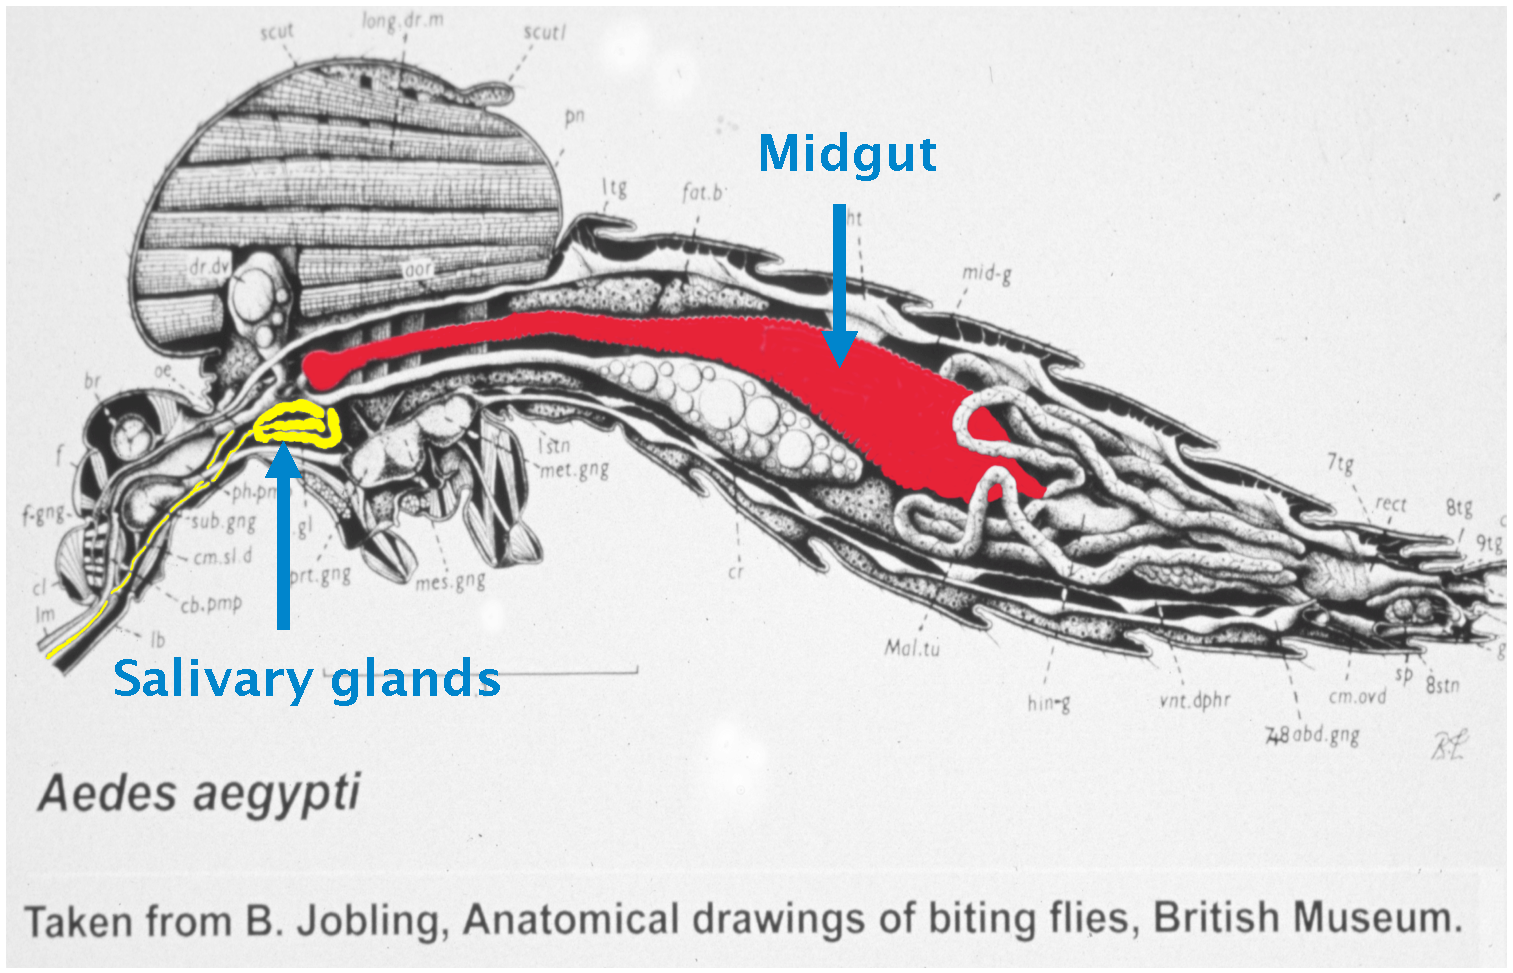
\includegraphics[width=.6\linewidth]{figures/figs/mosqXsection.pdf}
\caption[Cross section of a female mosquito]{\sf \textbf{Cross section of a female mosquito with tissues important to the transmission cycle highlighted.} \\  \cite{Jobling1987}}\label{fig:mosq-xsection}
\end{figure}


While the specifics of how viruses and protists live and reproduce in mosquitoes and humans are quite different, the transmission cycles of dengue and malaria are very similar in their critical events.
The transmission cycle of either pathogen type can be encapsulated into five fundamental events.
First, a female mosquito feeds on an infected human's blood taking up the pathogen as well (Figure \ref{fig:mosq-xsection}).
The bloodmeal is digested in the mosquito's midgut, and escape from the midgut is the first crucial step for the survival of the pathogen inside the mosquito.
If it is trapped in the midgut, it will eventually be passed as waste after the bloodmeal is digested.
If it manages to escape to the \gls{hemolymph}, the pathogen must survive long enough to gain access to the mosquito's salivary glands.
If it is unable to infiltrate the salivary glands, then the mosquito, while itself \textbf{infected}, is not \textbf{infectious} to other humans.
For this, the pathogen must be injected into the bloodstream of the next human along with the contents of the mosquito's saliva.

\section{Public health: \emph{multiple targets}}

Because the arrows of transmission essentially\footnote{While some mosquito
  to non-human vertebrate transmission may occur, it is not thought to
  be sufficient to maintain the pathogen if the mosquito:human loop is
  broken (\CITEME).}
points from mosquito to human or from human to mosquito, the cycle will collapse and a local area would eventually be cleared of the pathogen if either of those arrows are broken, provided that the intervention is maintained.
This model suggests two primary targets for public health interventions aiming to reduce the \gls{incidence}
(followed by \gls{prevalence}) of infection in a population:

\begin{enumerate}
\item Prevent mosquitoes from infecting humans.
\item Prevent humans from infecting mosquitoes.
\end{enumerate}

However, many interventions can not be clearly divided into addressing purely the human or vector side of the cycle.
For example, efforts to reduce the number of bites that humans receive from mosquitoes affects both the probabilities of the vector \emph{and} the human becoming infected.
This is one reason that vector control is almost always part of prevention strategies \CITEME.
For the purposes of this document, I will define human-based interventions to be those that are directly administered to a human body.
Essentially: medical interventions.

In this respect, the long term goals of public health are more focused on prevention than the treatment of acute cases.
Of course sick people need to be treated. Additionally, identifying and curing people who are infected also prevents mosquitoes from acquiring the pathogen as well.
However, in the long term prevention is preferred.


\subsection{Addressing the human side of the cycle}

Because of the definition of human-based interventions above, there are relatively few effective options in this category for malaria and dengue fever.
Normally, this section would include vaccines and swift, effective patient identification and treatment to clear the infection.
However, at this time these types of interventions simply do not exist on the market or in a cost-effective form applicable to the isolated and impoverished areas that are most affected \CITEME.

\subsection[Addressing the vector side of the cycle (conventionally)]{Non-transgenic options for addressing the vector side of the cycle}

Medical options are scarce generally in the regions of the world where these diseases are most common.
The alternative is to focus attention toward controlling access of the vector populations to human contact.
This can include removal of nearby mosquito breeding sites (usually various forms of standing water), spraying of insecticides, introduction of biological predators, and/or bed nets, etc.
One fairly recently developed approach that has shown great promise is \gls{SIT}.



\subsubsection{Sterile insect technique}
\gls{SIT} exploits a peculiar aspect of some insects' reproductive behavior. 
In many insects, the first mating event provides the only genetic material that the female will use to fertilize her eggs for the rest of her life \CITEME.
Subsequent mating events contribute little to no genetic material to the females progeny, \textbf{even if the first event involves a sterile male}.
This means that inundative numbers of sterilized males introduced into a native population will effectively sterilize significant proportions of wild females.
This has dramatic effects on the local population.
Negative population growth results from the inability of each generation to fully replace itself, and the effect is compounded for each subsequent generation as long as the program is maintained.
Perhaps most famously, \gls{SIT} was used successfully to eradicate the screwworm from the southern United States in the 1950s \cite{Bushland1955}.


\subsection[Transgenesis provides new vector control strategy]{Transgenic techniques provide a new strategy for controlling disease transmission}

Most conventional vector control strategies involve what might be termed vector \gls{population-reduction}.
In addition to population reduction, transgenic techniques provide a novel vector control strategy that has considerable implications to the sustainability of the vector control aspect of public health interventions for dengue and malaria.
In contrast to population reduction, this novel strategy could be conceptualized as vector \gls{population-conversion}.
It's goal is not to reduce or eliminate contact between humans and vectors but to drive a transmission-refractory trait through the vector population that renders the vector unable to become infectious at all, converting it into a non-vector.

\section{Elements of a successful transgenic vector control product}

\begin{enumerate}
  \item the ability to introduce transgenes into the vector genome in a heritable way
  \item the discovery or construction of effector genes
  \item the ability to control when and where the effector genes are expressed
  \item the ability of your transgenic vectors to have swift, dramatic, and clinically meaningful effects on the native vector population (gene drive)
\end{enumerate}



\subsection{Introducing heritable transgenes into mosquito genomes}

Before one can employ transgenic methods for vector control, one must have the capacity to make transgenic vectors.
For mosquitoes, this is more labor intensive than for other fly species like \Dmel.
However, it has been accomplished, and protocols to reliably introduce transgenes into many mosquito species now exist \CITEME.
Unfortunately, the relative difficulty is high.
It takes roughly 2-3 months to establish a stable line.
Thus many experimental approaches that are straightforward or even routine in \Dm or other species remain impractical for mosquitoes.

The method of introducing a \gls{transgene} into a mosquito genome generally relies on re-purposing the activities of \glspl{transposon} (\glspl{transposable-element}).
These nucleotide elements have the ability to cut themselves out of one part of the DNA and re-insert themselves into another.
It is possible to engineer them to insert selected transgenes into the mosquito genome instead of the genes that they usually contain.


Until recently, most if not all transposons used for transgenesis in mosquitoes inserted the transgenes into more-or-less random locations.
The number of locations and number of copies at any \textbf{single} genomic location was unpredictable \cite{Adelman2004,Sethuraman2007}.
This makes characterization of the effects of a transgene complicated.
However, with the successful implementation of the \gls{phic31} site-specific integration system in \Aa\ and \As\ \cite{Thorpe1998,Nimmo2006,Isaacs2012}, we can now reliably target specific, pre-characterized regions of these genomes for transgene integration of a single copy.

Heritability is achieved through specifically targeting the \gls{germline} cells of mosquito embryos for transgenesis.
In flies like mosquitoes, the cells that will become the germline always position themselves at one end (or pole) of the embryo (Figure \ref{fig:pole-cells}).
The transgenesis cocktail containing the transgene construct is injected into the embryos where the pole cells are located.
This means that the first generation of mosquitoes that may contain the transgene in every cell of their body is \textbf{not} the injected generation but the progeny of the injected mosquitoes.


\begin{figure}[h]
\centering \sffamily

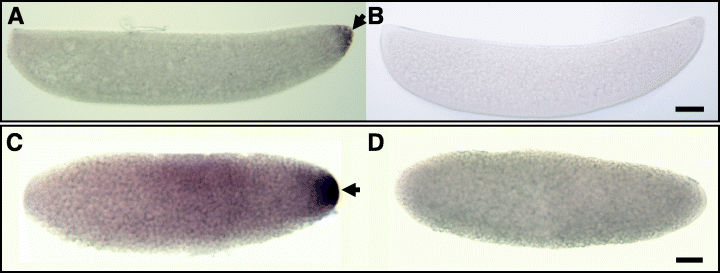
\includegraphics[width=.8\textwidth]{figures/figs/oskar_expression_AaAg.png}

\caption[\textit{oskar} gene expression in the vector mosquitoes, \Ang\ and \Aea]{\sf \textbf{\textit{oskar} gene expression in the vector mosquitoes, \Ang\ and \Aea:} \\
 Hybridizations \textit{in situ} of \textit{Anga osk} and \textit{Aeae osk} RNA probes to whole-mount \Ag\ and \Aa\ embryos. Embryos are orientated with anterior on the left. \Ag\ embryos (A,B) shown have reached cellular blastoderm with pole cells indicated by an arrow. \Aa\ embryos (C,D) shown are in the preblastoderm stage. Strong staining is exclusive to the posterior pole cells (A) and posterior end (C) (arrows), when compared with embryos of the same stage, determined by DAPI staining (not shown), probed with \textit{Anga} and \textit{Aeae osk} sense RNA probes (B,D). Bar = 50 µm.\\
 
 Excerpted from \cite{Juhn2006}}\label{fig:pole-cells}
\end{figure}

\subsection{Effector genes}

In addition to the ability to integrate transgene constructs into the vectors' genomes, it is necessary to design constructs that contain transgenes that will effect a useful response in the vector.
Two broad strategies are commonly applied when designing an anti-transmission phenotype: \gls{population-reduction} and \gls{population-conversion}.

\subsubsection{Vector population reduction:}

The goal of vector population reduction is the same as conventional vector control modalities.
\emph{Reduce the local population of a disease vector with the goal of reducing the probability that an infectious individual will have an opportunity to participate in a transmission event.}


A \textbf{transgenic tactic} for the population reduction strategy is illustrated by Oxitec's \Aa strain OX3604C developed with support from the Bill and Melinda Gates Foundation's Grand Challenges for Global Health Initiative.
Strain OX3604C represents a female-specific \gls{RIDL} approach which uses a poison transgene that kills any female adult expressing the transgene unless the female is provided an ``antidote'' through its water supply \cite{WisedeValdez2011,Bargielowski2012,Facchinelli2013}.

Releasing enough of these mosquitoes will affect the local mosquito species population in a way that is analogous to \gls{SIT}.

\subsubsection{Vector population conversion:}

Vector population conversion is a novel strategy for vector control that primarily exists within the context of genetically altered vectors (\CITEME wolbacia).
It promises to be the most long-lasting vector-focused intervention.
Unlike \textbf{all} vector population reduction tactics, there is a practical point in a conversion intervention (the anti-transmission trait works and is present in local populations at near 100\%) when the human management of the intervention can be ceased, yet it continues to function.
For population reduction to approach this result, the vector species must not simply be eliminated from the local area, but approach elimination on a continental scale, or more realistically achieve global eradication.

The reason is that these mosquitoes (especially \Aa) can and do travel long distances, as eggs or larvae, in the backs of trucks (between villages) or in the pools of water collected in super-tankers (transcontinentally).
So a local village is only free of the vectors until more migrate into the area.
But in a conversion scenario, those migrants mate with the local vector population, and their offspring are assimilated into transmission-deficient mosquitoes.
The protection of the local village can be preserved \emph{even if some surrounding villages fail to maintain control of their mosquitoes}.

An example of a \textbf{transgenic tactic} for population conversion of \Aa\ into a transmission-deficient phenotype involves an effector gene that produces a double stranded RNA molecule that contains a portion of the dengue virus genome \cite{Franz2006,Mathur2010}.
Because most animal cells have a system that detects and degrades double stranded RNA\footnote{Double stranded RNA generally signals that a virus is active in the cell.}
in a sequence specific manner, this primes the mosquito cells' antiviral response to specifically attack the dengue virus if the effector gene is expressed in the cell before it gets infected.

\subsection{Controlling when and where the effector genes are expressed}

Even with an effector gene that clears 100\% of the pathogen 100\% of the time, the intervention will not be successful in limiting transmission if the transgene is not turned on at the right time and place.
If the transgene is most effective when the pathogen is in the midgut, it is not useful if the gene is only expressed in the antennae.

The region of DNA directly before the sequence of the gene is a major determinant of the pattern of expression and is referred to as the promoter.
It influences when the gene will be turned on (e.g., directly following the ingestion of a bloodmeal), and in which tissue type (e.g., the midgut).
Promoters influence the transcription of genes through the binding of special proteins called transcription factors that recognize specific DNA sequences called \glspl{CRE}.
\glspl{CRE} are sometimes organized into modules that represent groups of binding sites for a specific combination of transcription factors.
These modules are \glspl{CRM} \CITEME (Figure \ref{fig:cre-crm-intro-a}).
Once a set of transcription factors are bound to the promoter they recruit the special machinery needed for the gene to be turned on or silenced depending on the context of the cellular environment (Figure \ref{fig:cre-crm-intro-b}).



\begin{figure}[h]

\begin{subfigure}[b]{.5\linewidth}
\centering 
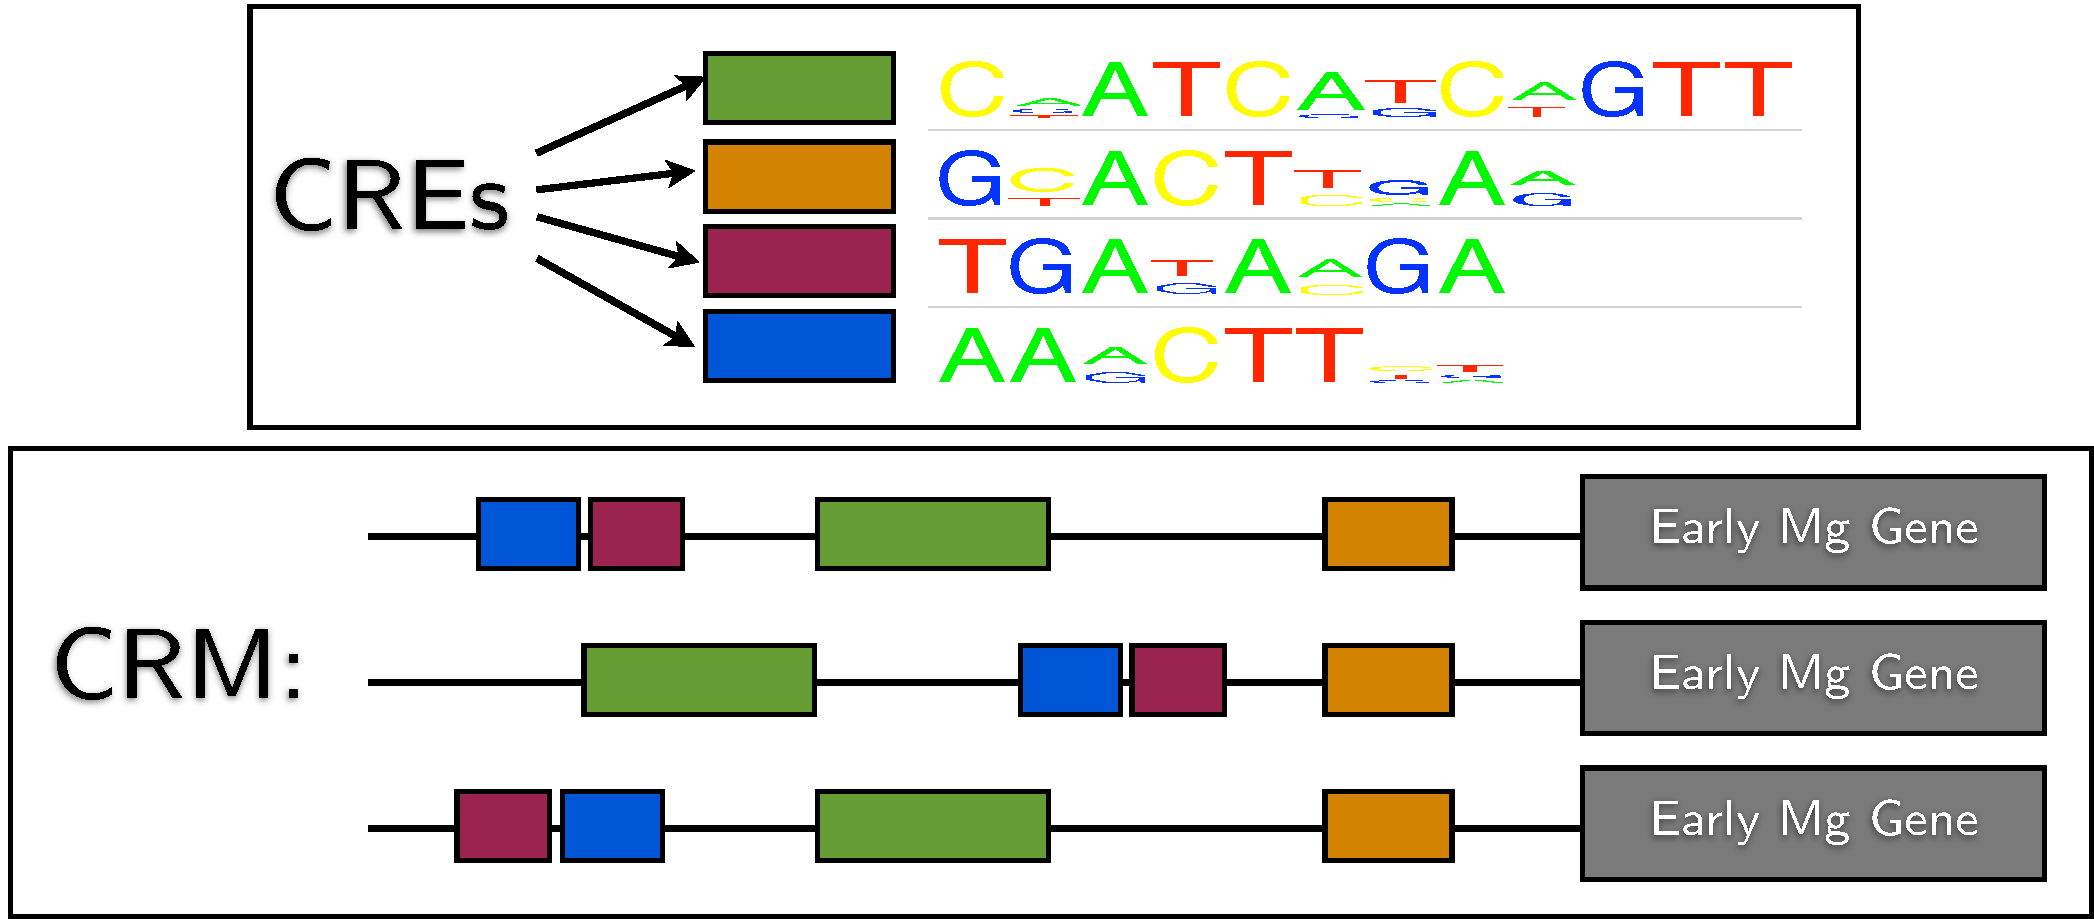
\includegraphics[width=0.9\linewidth]{figures/figs/CREvCRM.pdf}
\caption{}\label{fig:cre-crm-intro-a}
\end{subfigure}%
\hfil
\begin{subfigure}[b]{.5\linewidth}
\centering
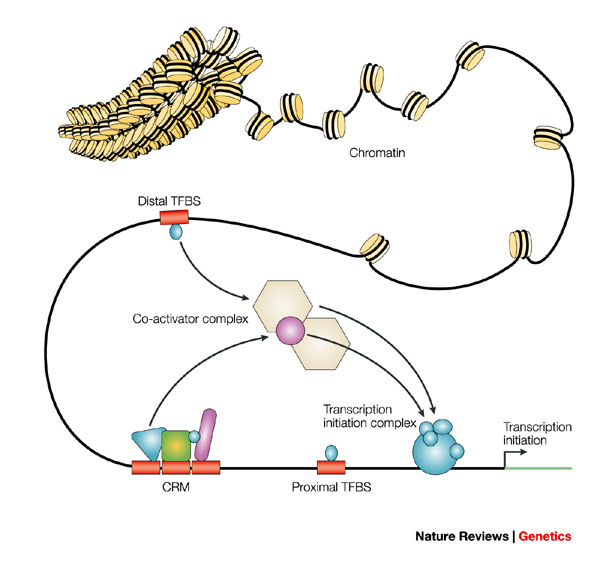
\includegraphics[width=0.9\linewidth]{figures/figs/elementsOfTxReg.jpeg}
\caption{}\label{fig:cre-crm-intro-b}
\end{subfigure}

\caption[Elements of transcriptional regulation]{\sf \textbf{Elements of transcriptional regulation} \\
(A) The relationship between \glspl{CRE} (colored rectangles) and \glspl{CRM}: the colored rectangles represent position specific scoring matrix information (top) that defines an individual \gls{CRE}.
(B) \glspl{TF} bind to specific sites (\glspl{TFBS}) that are either proximal or distal to a transcription start site. Sets of \glspl{TF} can operate in functional \glspl{CRM} to achieve specific regulatory properties. Interactions between bound \glspl{TF} and cofactors stabilize the transcription-initiation machinery to enable gene expression. The regulation that is conferred by sequence-specific binding \glspl{TF} is highly dependent on the three-dimensional structure of chromatin.\\

Panel B and corresponding legend text adapted from \citet{Wasserman2004}.
}\label{fig:cre-crm-intro}
\end{figure}

A typical strategy to obtain regulatory sequences suited to drive a transgene following the expression characteristics used as an example above (expressed directly following ,a bloodmeal, in the midgut) would be to identify genes in the mosquito that already have a similar expression pattern to the ideal.
The promoter from that gene would then be copied and inserted in front of our transgene in the final integration construct.

This is a very common process used to engineer the expression patterns of real transgenes in mosquitoes.
In \cite{Moreira2000}, the promoter sequences of a gene called carboxypeptidase (normally expressed in the midgut after a meal) from \Aa\ and \Ag\ were inserted in front of a reporter gene.
The result was luciferase mRNA and protein abundantly expressed in the midguts of transgenic mosquitoes in four of six AeCP lines and in the.
Expression of the reporter gene was gut-specific and peaked about 24h \gls{PBM}.


\subsection{Achieving swift, dramatic, and clinically meaningful effects on the native vector population}

In many ways, this is the most difficult part of the system.
In order for the transgene to have its self-sustaining properties as well as achieve effective anti-transmission results, it must spread through the native mosquito population to the point that the percent of individuals possessing the gene approaches 100\%.

Making the optimistic assumption that the transgene carries a negligible fitness cost
\footnote{By fitness cost/advantage here, I mean that the transgene
    causes the mosquitoes that inherit it to be either less or more
    successful at producing offspring, respectively.},
or even a slight fitness advantage, achieving near 100\% conversion could take decades.
Funding terms for efforts like this in poor nations can be closer to 5 years or less.
To enable the population conversion strategies to work, genetic ``tricks'' must be exploited that cause the gene to spread through a mosquito population \textbf{much} faster than could happen naturally.
Efforts to discover or design these \gls{gene-drive} systems are an on going and active area in this field.

An example of such a method is the Medea system successfully engineered in \Dm\ (\CITEME).

\textbf{In Brief:}
\begin{enumerate}
 \item The construct consists of a \textbf{death gene} under control of a maternal effect promoter and a \textbf{rescue gene} under control of an early embryonic promoter.
 \item The \textbf{death gene} is produced by the mother and deposited into 100\% of her developing embryos: \textit{even those that did not inherit the transgene due to mating with a wild type male.}
 \item However, since the \textbf{rescue gene} is produced by only those embryos that inherited the transgene construct, only those embryos will survive.
 \item The female has on average half as many progeny survive as usual if she mated with a wild type male, but 100\% of those that survive inherit the transgene.
 \item Over time this results in the fixation or near fixation of the transgene in the population.
\end{enumerate}


\section{Evolutionary relationship between mosquitoes and hematophagy}
\begin{quotation}
\textbf{Closely Related Lineages, Share Similar Sets of Protein Families
in Their Sialomes, Even If No Apparent Orthologous or Conserved
Functional Relationships Exist}
For example, while the D7-proteins in mosquitoes possess an extra alpha-helix
involved in the binding of biogenic amines, this helix is absent from the D7-proteins from sand flies and biting midges, implying that they will not possess biogenic amine-binding function (Mans et al., 2007).

Th\textbf{e Same Protein Families are Prone to Expansion in Closely Related Lineages}
The odorant-binding/D7-family expanded in mosquitoes, sand flies and bitingmidges (Anderson et al., 2006; Campbell et al., 2005; Francischetti et al., 2002a).

Excerpted from \cite{Markland2011}
\end{quotation} 

\todo[inline]{expand how the evolutionary relationship between hematophagy and mosquitoes may be useful}
\dummytext[3]

\subsection{Implications for design of transgenic vector control systems?}
\todo[inline]{write the implications your work will have on designing transgenic vector control systems}
\dummytext[3]


% \briefConclude{
% \begin{itemize}
% \item there are many but we focus on Dengue Fever and Malaria
% \item causative agents are RNA viruses and Plasmodium protists, respectively
% \item people don't give people these two diseases
% \item mosquitoes generally don't give mosquitoes these diseases
% \end{itemize}
% }
% \synopsis{
% \begin{itemize}
% \item The specifics of the transmission cycle of these diseases provides multiple targets for public health interventions
% \item focus on the human
% \item focus on the vector
% \end{itemize}
% }
\chapter{Review of Pertinent Publications}
%\todo[inline]{replace CITEME tags in Development of Rationale and Review of Published Works}

Our previous attempts to infer \glspl{CRE} bioinformatically have been relatively successful.
Comparative genomics by way of the \gls{MDOS} program allowed us to infer a set of k-mers that should represent \glspl{CRE} conserved among three species of mosquitoes (\Aa, \Ag, \Cq).
This method used no expression information in the process of predicting the \glspl{CRE}.
However, we were able to show that a sub-set of the inferred \glspl{CRE} were enriched significantly in abundance profiles derived from a previous affymetrix-based bloodfeeding experiment in \Ag\ \cite{Marinotti2005},\cite{Marinotti2006},\cite{Sieglaff2009}.
Comparing transcriptional abundance profiles between sugarfed and bloodfed (5h \gls{PBM}) \Aa\ mosquitoes allowed us to predict multiple putative \glspl{CRE} when we focused on transcripts that were detected at high levels in in bloodfed mosquitoes but undetectable in sugarfed females \cite{Bonizzoni2011}.
Possible \glspl{CRM} were observed by visual inspection as well, but efforts to confirm biological meaningfulness have not yet been completed.
Putative \glspl{CRM} were again observed by visual inspection in an experiment comparing mRNA abundance profiles between \Aa\ fed with blood infected with dengue virus and those fed with non-infected blood.
In this study, specific tissues were dissected and analyzed separately providing a level of tissue specificity as well.
These \gls{CRM} results also remain in the process of being confirmed experimentally.

These studies have provided useful lessons that I have incorporated into the approach described in Chapter \ref{chap:3}.
A common theme among these lessons is the importance of the relative ratio of signal-to-noise contained in the data-set being examined.
For example, in \citet{Bonizzoni2011}, the most successful \gls{CRE} prediction results arose from a gene-set characterized by a fairly restrictive abundance profile definition (the requirement that transcripts be detected highly at 5h \gls{PBM} but completely undetectable in sugarfed mosquitoes).
This yielded a gene-set of just 40 members.
\citet{bonizzoni2012complex} further demonstrates that \gls{functional genomics} results are sensitive to the definition of gene-sets used for analysis.
In addition to abundance profile definition, \citet{Bonizzoni2011} illustrated that, in \Aa, the official annotation is incomplete and contains at least some level of annotation errors that may be considered particularly troublesome to analyses that rely on accurate definition of putative promoter sequences; however, it also provides support that, despite containing errors, the current state of annotation is sufficient to allow \gls{CRE} prediction.
Finally, in experiments comparing mRNA abundance profiles between three different strains of a single species (\Aa), \citet{bonizzoni2012strain} illustrates the need to take precautions when comparing differences in transcript abundance profiles between species that are estimated to have last shared a common ancestor as long as 200 \gls{Mya}.


\section{Comparative genomics allows the discovery of \textit{cis}-regulatory elements in mosquitoes. \cite{Sieglaff2009}}

\begin{figure}[hp]
\centering

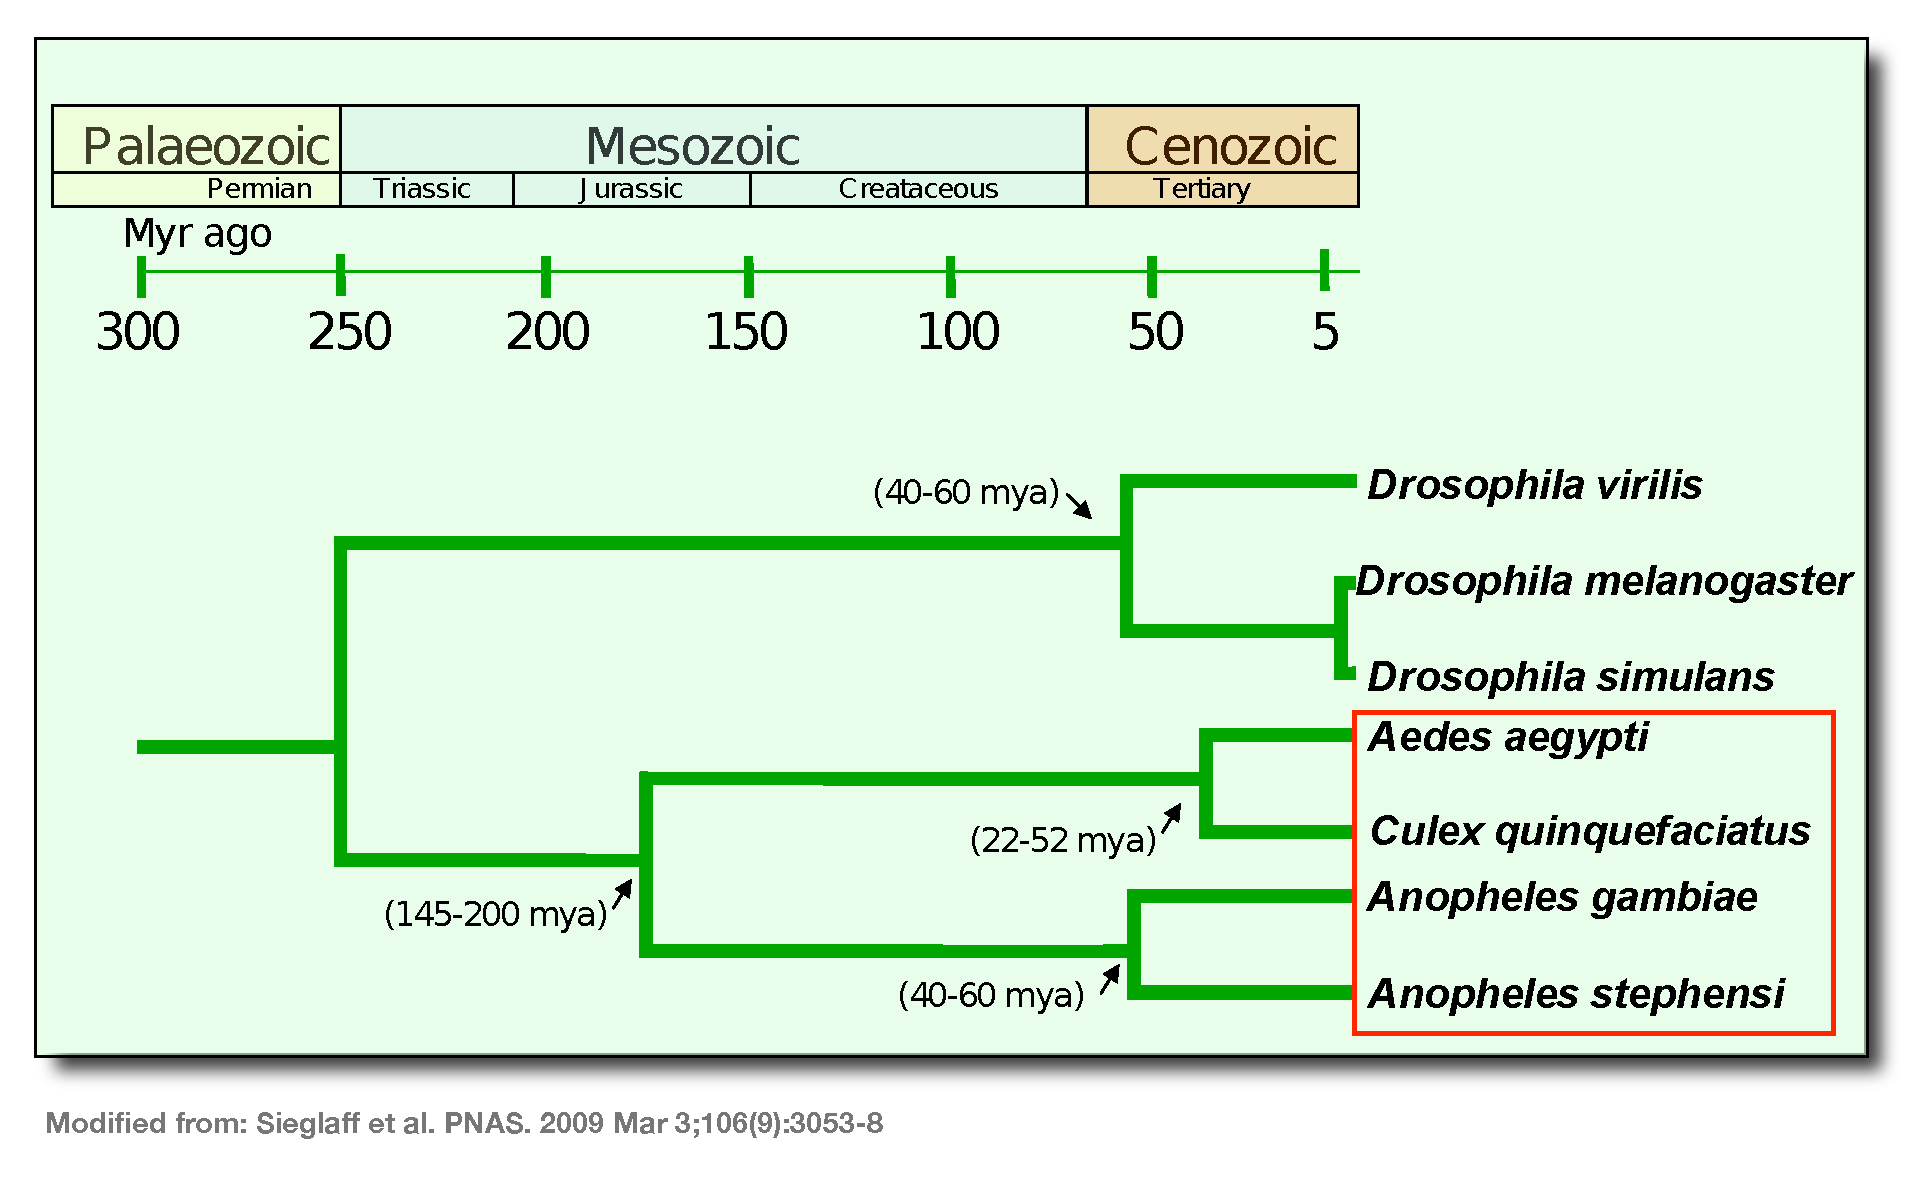
\includegraphics[width=.7\textwidth]{figures/figs/mosqPhyloTree.pdf}

\caption[Phylogenetic relationships between four vector mosquitoes]{\bsf{Phylogenetic relationships between four vector mosquitoes compared with representative \textit{Drosophila} species:} \\ \sf
\dummytext[1]

Adapted from \cite{Sieglaff2009}}
\label{fig:mosqPhyloTree}
\end{figure}

\begin{figure}[hp]

\hfil
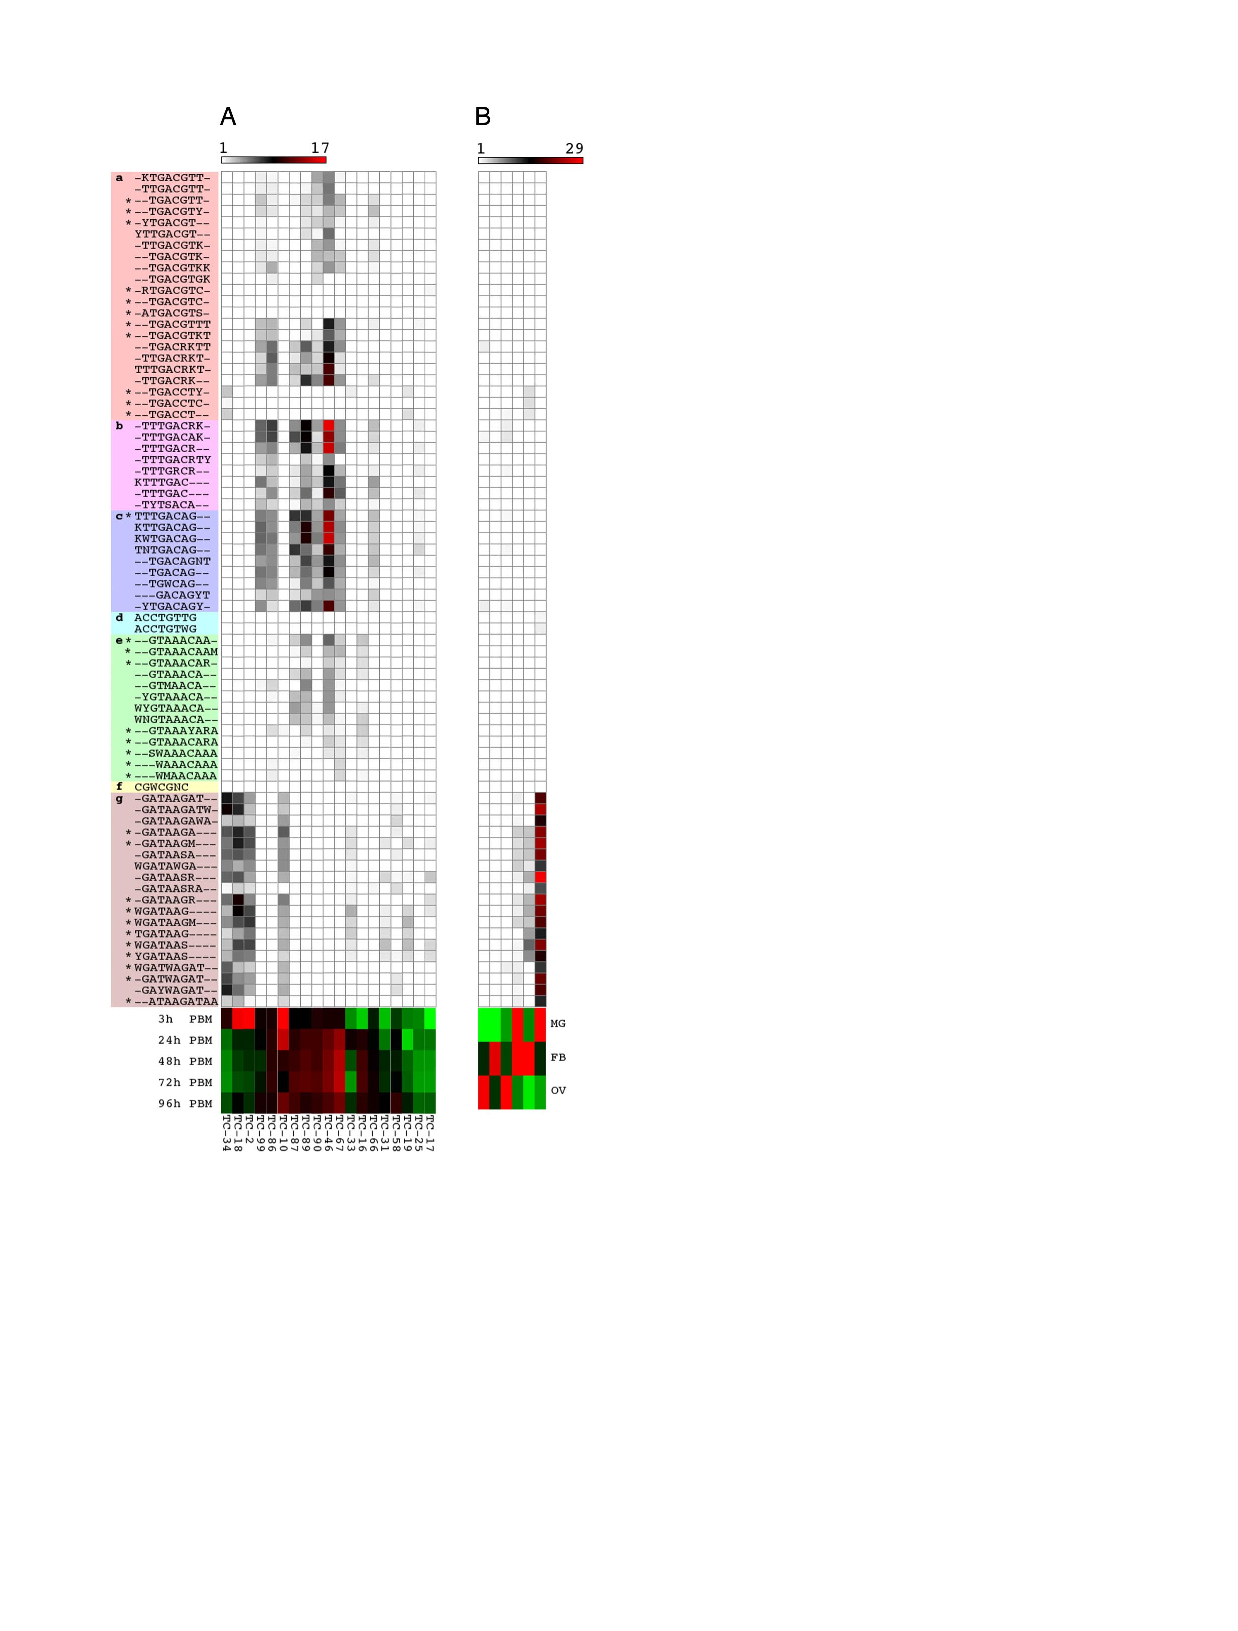
\includegraphics[scale=.95]{figures/figs/sieglaff2009_full.pdf}
\hfil
\caption[Associations of mosquito motifs with gene expression profiles in \Ag]{\bsf{Associations of mosquito motifs with gene expression profiles in \Ag:} \\ \sf
Motif enrichment within (A) 5′-end flanking regions of genes in clusters responsive to blood meal ingestion, and in (B) 5′-end flanking regions of genes in clusters enriched in selected tissues. The significance of motif enrichment is indicated by pseudocolor of -log10 (P-value) determined through hypergeometric statistics, and the median expression profile of each gene cluster is shown below each respective column. Red and green colors represent higher and lower relative mRNA accumulation, respectively. Asterisks (*) indicate a match to a previously described mosquito TFBS. Heatmaps were created with Matrix2png (\CITEME:local-58). FB, fat body; hPBM, hours post blood meal; MG, midgut; OV, ovaries; TC, time course clusters.

Adapted from \cite{Sieglaff2009}}
\label{fig:sieglaff2009_full}
\end{figure}

% [*\CITEME 3]  \cite{Nene2007}
% [*\CITEME 10] \cite{Wu2008}
% [*\CITEME 25] \cite{Kokoza2001}
% [*\CITEME 26] \cite{Cho2006}
% [*\CITEME 28] \cite{Attardo2003}
% [*\CITEME 29] \cite{Ahmed1999}
% [*\CITEME 30] \cite{Pham2005}
% [*\CITEME 32] \cite{Giannoni2001}
% [*\CITEME 33] \cite{Davidson2010}
% [*\CITEME 34] \cite{Das2007a}
% [*\CITEME 35] \cite{Hu2005}
% [*\CITEME 36] \cite{Tompa2005}
% [*\CITEME 37] \cite{Wasserman2004}
% [*\CITEME 38] \cite{Elemento2005}
% [*\CITEME 39] \cite{Stark2007}
% [*\CITEME 40] \cite{Xie2005}
% [*\CITEME 41] \cite{Dittmer2003}
% [*\CITEME 42] \cite{Meredith2006}
% [*\CITEME 43] \cite{Hernandez-Romano2008}
% [*\CITEME 44] \cite{Rai1999a}
% [*\CITEME 45] \cite{Borkent2004}
% [*\CITEME 46] \cite{Calvo2006}
% [*\CITEME 47] \cite{Adelman2007}
% [*\CITEME 48] \cite{Xu2005a}
% [*\CITEME 49] \cite{Jasinskiene2007}



The role \glspl{CRE} play in regulating gene expression during development is well-established \cite{Davidson2010}, and the development of tools for their identification is an active area of research following the publication of genome sequence and associated genome-wide expression datasets. However, the discovery \textit{in silico} of \glspl{CRE} is challenging because typically they are short, degenerate, and contained within vast amounts of intergenic genomic DNA. Despite these limitations, various computational approaches have been developed for their discovery \cite{Das2007a,Hu2005,Tompa2005,Wasserman2004}. Comparative genomics represents a powerful extension to \gls{CRE} discovery that diminishes these effects. Functional gene regulatory elements, including \glspl{CRE}, are proposed to diverge at much lower rates compared to neutral sequences because of selective pressures, and therefore may stand out from surrounding neutral DNA by virtue of their greater levels of conservation among orthologous sequences. Previous work has demonstrated the utility of this concept \cite{Elemento2005,Stark2007,Xie2005} and comparative genomics of insects has been applied successfully to map putative \glspl{CRE} in the genomes of relatively closely related \textit{Drosophila} species, [divergence times estimated ≤ 50 \gls{Mya} \cite{Stark2007} (Figure \ref{fig:mosqPhyloTree})], in which orthologous intergenic sequences are aligned more easily. The work represented by \citet{Sieglaff2009} includes mosquito species with phylogenetic relationships spanning 20 to 200 \gls{Mya} with genomic comparisons complicated by large amounts of dispersed repetitive elements \cite{Nene2007}.

The \gls{MDOS} algorithm \cite{Wu2008} was designed to mitigate these problems by not requiring alignment of orthologous sequences, and incorporating features that account for the greater probability for the co-occurrence of a motif because of shared ancestry in orthologous sequences. The application of \gls{MDOS} for computational discovery of putative \glspl{CRE} shared among mosquitoes resulted in the identification of mosquito-specific or enriched motifs. These motifs demonstrate that \gls{MDOS} can identify related DNA sequences in diverged mosquitoes and may be useful in similar scenarios in which genome sequences are being analyzed for species that have no other closely related genomes available. Furthermore, the identification \textit{in silico} of GATA-factor and other \glspl{TFBS} that are identical to those whose function was established experimentally \cite{Kokoza2001,Cho2006,Attardo2003,Ahmed1999,Pham2005,Giannoni2001,Dittmer2003,Meredith2006} serves as a powerful positive control for these analyses. The 5′-end regions of immune-related genes from \Ag\ and \Dm\ were screened for conserved motifs, and AT-rich domains were found to associate with \gls{NFKB} response elements \cite{Hernandez-Romano2008}. These sequences were not identified in these analyses because the restrictions on the dataset used eliminated many of the immune-related genes where one-to-one orthology may be difficult to establish. In addition, most AT-rich domains discovered in their study were ≤ 6 nucleotides in length, and these analyses only addressed those recovered with lengths of 7 to 9 nucleotides.

The 3 mosquito species included in \citet{Sieglaff2009} require a bloodmeal for successful reproduction. Although this trait is not unique to this group of arthropods, acquiring the necessary nutrients for egg development from ingested blood is a specialized adaptation in insects. There is debate on when and how \gls{hematophagy} arose in mosquito evolution \cite{Rai1999a}, but it is hypothesized that the occurrence of this trait in the larger clade is \gls{monophyletic} \cite{Borkent2004,Calvo2006}. Most of the discovered mosquito motifs are associated with bloodmeal-regulated genes. Thus, these data support a common hematophagous ancestor for all mosquitoes, and indicate that \gls{hematophagy} acts as a selective force for conservation of \glspl{CRE}.

The functionality of some of the discovered motifs was supported further in \Ag\ and \Aa\ by their association with genes displaying enriched transcription product accumulation within tissues responsible for bloodmeal digestion and reproduction (Figure \ref{fig:sieglaff2009_full}). These findings bolster the conclusion that these mosquitoes share a regulatory code controlling expression levels for some genes regulated after \gls{hematophagy}. The availability of additional genome-wide studies of gene expression for all 3 mosquito species will facilitate discovery of other associations of the motifs with specific gene-regulation patterns.

\citet{Sieglaff2009} and similar genome-wide approaches to identify putative \glspl{CRE} in mosquitoes \cite{Hernandez-Romano2008} are furthering our understanding of the mechanisms involved in gene regulation in this group of vector insects. An expanded set of putative mosquito \glspl{CRE} will allow the definition of genome-wide motif-association maps and the identification of \glspl{CRM} comprising multiple, linked \glspl{CRE} that convey specific patterns of gene expression. Experimental validation of the functionality of each discovered motif and regulatory module is necessary and will provide support for the development of mosquito synthetic promoters that deliver desired and predetermined expression patterns in transgenic mosquitoes. 
The availability of defined synthetic mosquito promoters that direct controlled, local gene expression in response to pathogens also would be a major advance. These promoters would allow engineering of mosquitoes with increased parasite or virus resistance. These and similar envisioned applications for mosquito control and the control of mosquito-borne disease transmission will benefit greatly from a better understanding of gene regulation mechanisms in these insects.










\pagebreak

\section{RNA-seq analyses of blood-induced changes in gene expression in the mosquito vector species, \Aea\ \cite{Bonizzoni2011}}
% [-17] Brackney2010
% [-31] Fischer2008
% [-32] Pane2007
% [-33] Lawson2009
% [-50] Salazar2007
% [-54] Marelli2006
% [-55] Amenya2010
% [-56] Carlson2007
% [-57] Kriventseva2008
% [-58] Sieglaff2009
% [-60] Hubbard2002
% [-61] GENEBUILD?
% [-62] Bennet2002
% [-63] Black2002
% [-64] Terenius2008



Bonizzoni and Dunn \cite{Bonizzoni2011} provides a detailed examination of the changes in transcripts accumulation occurring at the whole-body level of \Aa\  females 5 hours \gls{PBM}. The observed changes are consistent with the beginning of an intense physiological response to a bloodmeal. The majority of immunity-related transcripts tended to accumulate at lower levels in bloodfed mosquitoes. This finding supports the hypothesis that there may be a gap in immunity following a bloodmeal. Reduced expression of immune genes in bloodfed mosquitoes could favor the establishment of infections, especially considering that pathogens such as dengue viruses infect the midgut epithelial cells within minutes after the contact \cite{Salazar2007}. However, changes in transcript abundance observed at the whole-body level may mask changes in accumulation occurring primarily in the midgut. Different levels of activation of immunity genes after a blood feeding may be one of the factors contributing to the variability in vector competence for dengue viruses observed in different geographic populations of \Aa\  \cite{Bennett2002},\cite{Black2002}. The quantity and quality of data generated by RNA-seq technology makes it an ideal approach for comparative analyses of the transcriptome of \Aa\ strains with different vector competence and vectorial capacity.

Our analyses of the expression profiles of sugarfed (S) and bloodfed (B) mosquitoes allowed the identification of co-regulated genes and putative \textit{cis}-regulatory elements and modules from the \Aa\  genome. Further knowledge of the mechanisms involved in regulation of gene expression in vector species is critical to the development of control strategies whereby the vector is modified genetically to express anti-pathogen effector molecules in tissue-specific and time-regulated manners \cite{Terenius2008}. Promoter and other \textit{cis}-acting regulatory DNA fragments are needed to regulate restricted expression of selected anti-pathogen effector molecules. Moreover, we described several examples of how the RNA-seq data generated can help improve the current annotation of the \Aa\  genome.

\subsection{Transcripts found exclusively in bloodfed mosquitoes}
Forty transcripts were found only in bloodfed mosquitoes, with the highest read-counts reaching ~1000/transcript, after normalizing for different library sizes (data not shown). Functional parent attribution for these transcripts is consistent with a role in digestion and in the progression of the gonotrophic cycle. Specifically, two transcripts, Aa5G1 (AAE013712-RA) and AaSPVI (AAE010196-RA), correspond to the midgut serine proteases shown previously to be elicited by a bloodmeal in the midgut of \Aa\  females \cite{Brackney2010}. Seven other transcripts encode enzymes (i.e. decarboxylase, cathepsin b and trypsins), and two are implicated in trafficking. Transcripts AAE014815-RA and AAE005950-RB correspond to the vacuolar protein sorting 13B from yeast and the chloride channel protein 2, respectively. Ten transcripts are orthologous to the G12 gene of \Ag\ and share the Insect Allergen Repeat motif. This motif is hypothesized to be a novel, insect-specific detoxifying domain implicated in the co-evolution of herbivorous insects and their plant hosts and also has been linked to nitrile-specific detoxification \cite{Fischer2008}. Transcripts AAEL006126-RB and AAEL008921-RC are predicted orthologues of the \Cxq\ vitellogenin-A1 gene and the \Dmel\ spaghetti squash (sqh) gene, respectively. The sqh gene product encodes the regulatory light-chain of non-muscle myosin II, which is required for cytoplasmic transport in nurse cells during oogenesis and also has been implicated in germline \gls{RNAi} processes \cite{Pane2007}.

\subsection{\textit{Cis}-regulatory element discovery}
Tightly regulated and bloodmeal-induced expression profiles are of particular interest for designing transgenic mosquito-based control strategies to reduce transmission of dengue fever. \textit{Cis}-regulatory sequences derived from bloodmeal-induced / up-regulated mosquito genes allow potentiating swift induction and effective levels of transcription of an associated effector gene, while likely inflicting the least fitness cost \cite{Marelli2006}, \cite{Amenya2010}. We interpret the different levels of mRNA accumulation seen in this study to reflect changes in transcriptional activity of the corresponding genes, although it is possible that some levels may vary as a function of changing transcript stability or rates of turnover. With this in mind, we used \gls{SCOPE} \cite{Carlson2007} to predict putative \glspl{CRE} that may provide the basis for rational identification and selection of new candidate promoter regions and for modification of the transcriptional profiles of current transgene constructs. We examined the 2000 base pairs (bp) flanking the 5'-boundaries of the 40 transcripts that were undetected in libraries from sugarfed mosquitoes but detected at significant levels in the RNA-seq libraries from bloodfed mosquitoes and identified a redundant list of 22 motifs that are enriched significantly in these sequences (Figure \ref{fig:bonizzoni2011-cres}). A possible \gls{CRM} constructed with the discovered \glspl{CRE} is represented by the motif consensus sequences, \texttt{cnatcnkcwgtt}, \texttt{gyactyvar}, and \texttt{tgakamga}, and is associated with \Aa\  orthologs of the G12 gene of \Ag\ (AGAP006187) (Figure \ref{fig:bonizzoni2011-cres}). \Aa\ has 17 G12 genes, many more relative to other insects, which have 4.5 on average (according to OrthoDB; group EOG95TCTG) \cite{Kriventseva2008}. The transcripts of nine of the G12 orthologs are present in this co-regulated gene set (representing ~25\% of the 40).

Another putative \gls{CRM} contains the consensus sequence \texttt{tgakamga}, \texttt{cnatcnkcwgtt}, \texttt{asttrccc} and \texttt{aarcttbd} (Figure \ref{fig:bonizzoni2011-cres}). This \gls{CRM} groups with the cathepsin b genes, AAEL015312-RA and AAEL007585-RA. Verification of these \glspl{CRM} will require empirical testing, however, the top 10 matches for \texttt{tgakamga}, which is present in both putative \glspl{CRM}, align well to members of the mosquito-conserved GATA motifs correlated to transcriptional responses to blood feeding in \Ag\ \cite{Sieglaff2009}.





\subsection{RNA-seq identifies annotation corrections}


\begin{figure}[hp]
\centering
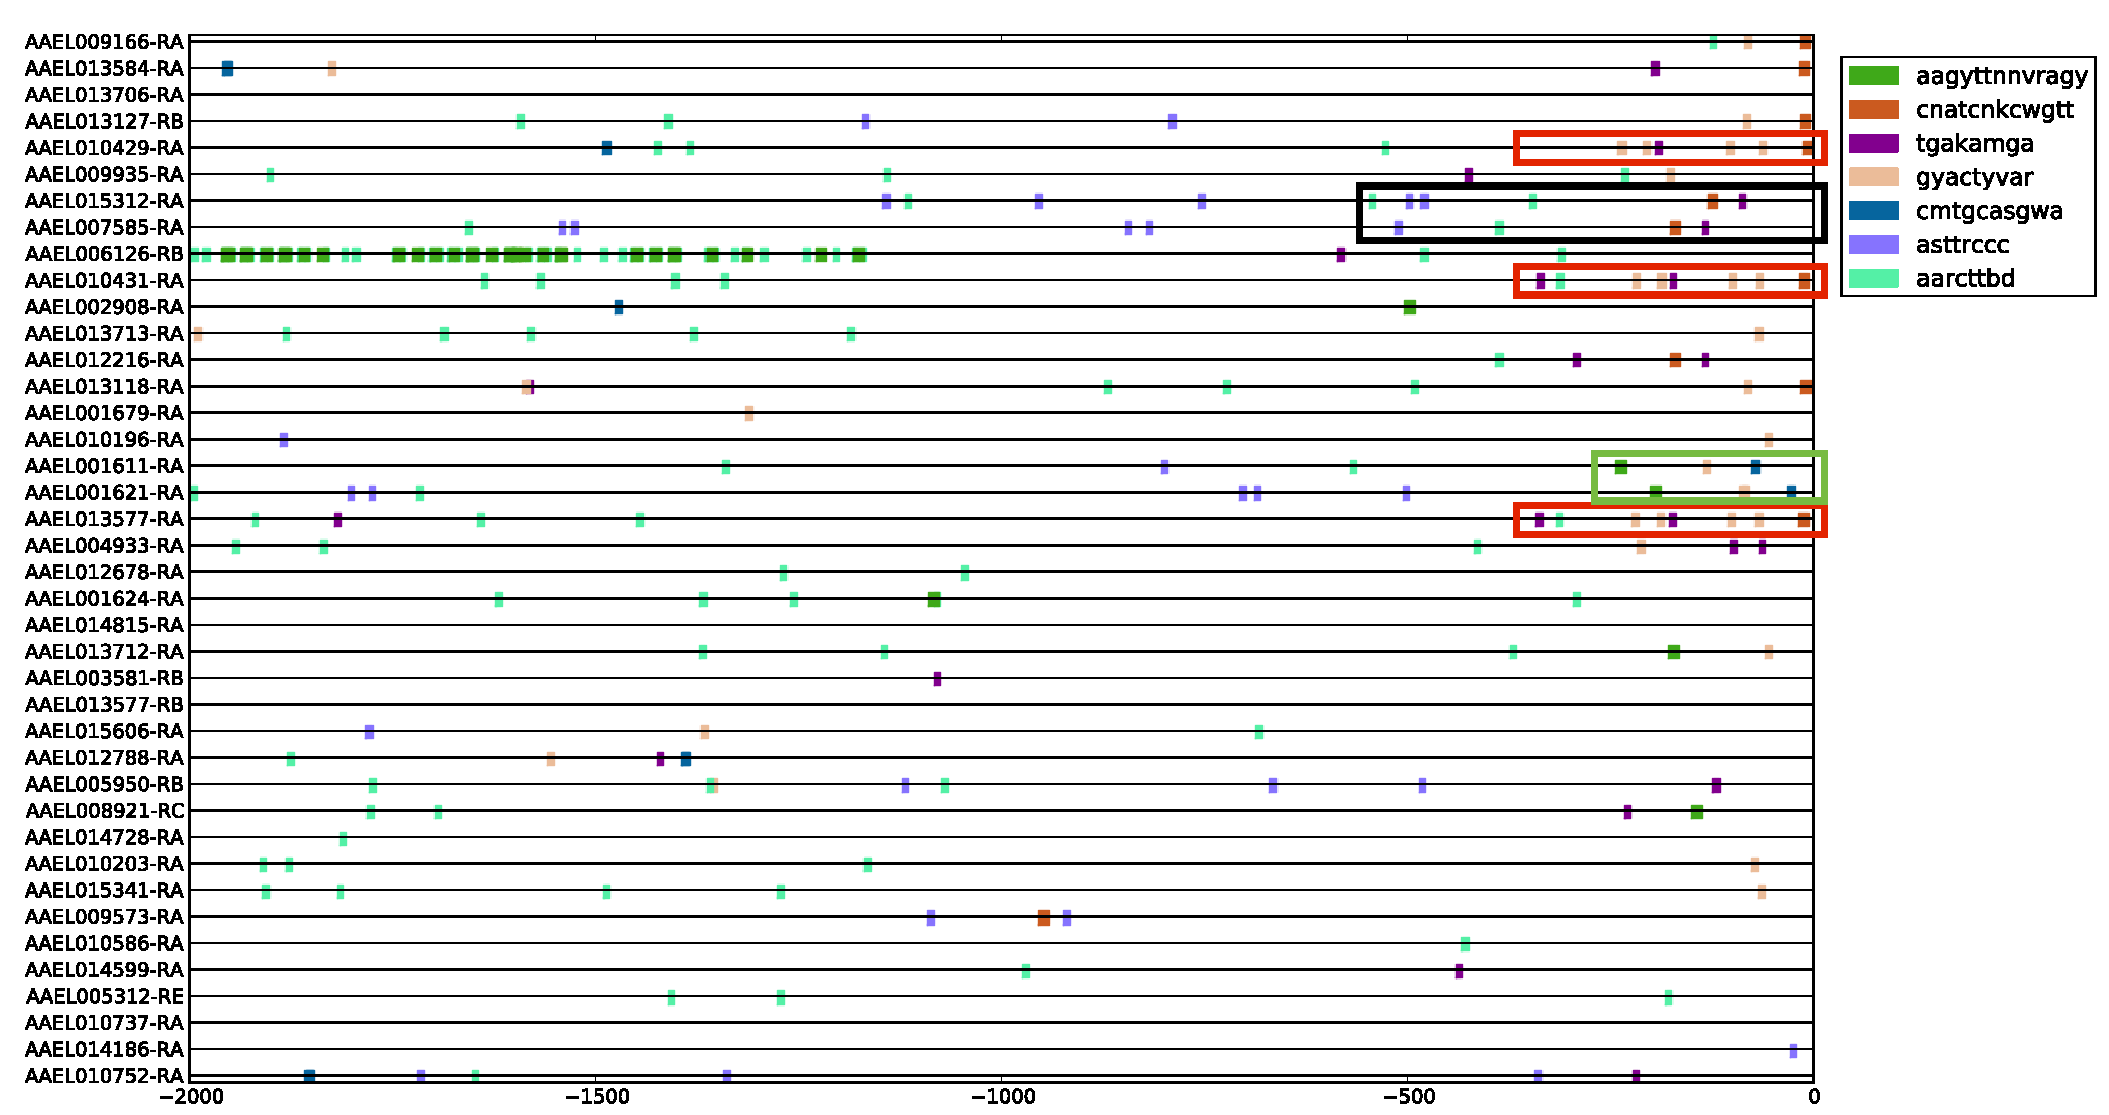
\includegraphics[width=.99\textwidth]{figures/figs/bonizzoni2011-cres.pdf}

\caption[Motif map of putative CREs from transcripts detected only in bloodfed female \Aa]{\sf \textbf{Motif map of putative CREs discovered by SCOPE using transcripts detected significantly only in bloodfed female \Aa:} Locations of representative SCOPE-derived CRE motifs in the 2000 bp upstream of the annotated translational start site in the 40 transcripts detected significantly only in bloodfed females. Transcript names on the left are ordered from most (top) to least (bottom) abundant.  Candidate CRMs are highlighted in like-colored rectangles.

Adapted from \cite{Bonizzoni2011}}
\label{fig:bonizzoni2011-cres}
\end{figure}

\begin{figure}[hp]
\centering
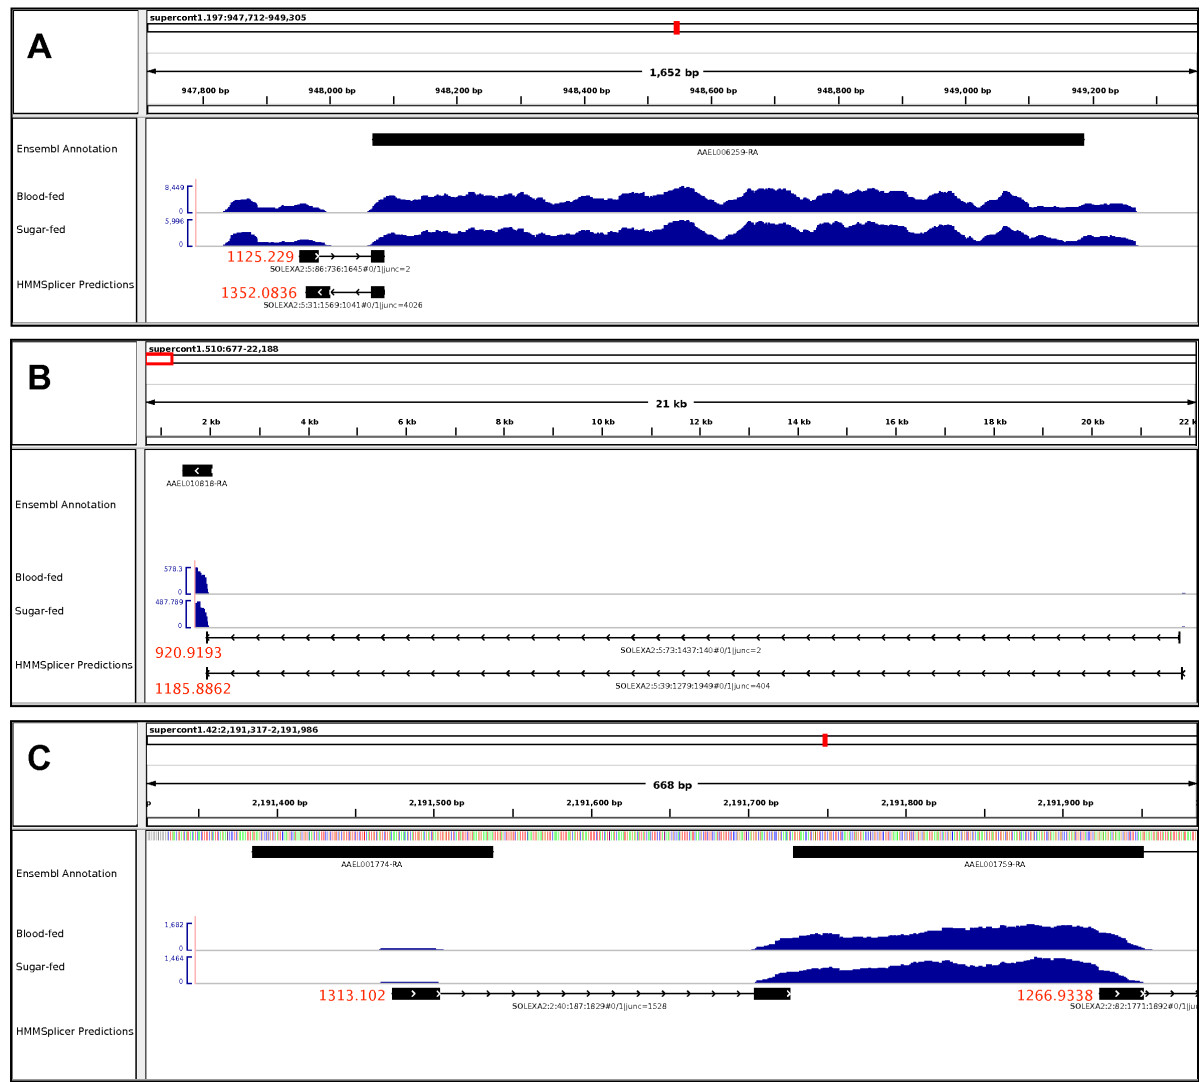
\includegraphics[width=.95\textwidth]{figures/figs/aedesHMMsplice.jpg}

\caption[Examples of amendments to the \Aa\ annotation supported by HMMSplicer results]{\sf \textbf{Examples of amendments to the \Aa\ annotation supported by HMMSplicer results:} Black bars in the top tracks represent the current gene annotations. Blue histograms in the second track represent the non-normalized coverage of RNA-seq reads at each position. The range of the histogram values shown in each view is depicted on the labeled y-axis of each RNA-seq track. Black boxes in the lower track represent splice-site predictions based on the RNA-seq reads using HMMSplicer determined in this study. Each function has a unique identifier listed below and its HMMSplicer score is listed in red. If multiple reads support a single junction, "junc = x" lists the number of supporting reads. This information provides evidence to link two islands of transcription as a single transcription event, therefore, exons of a common mRNA. All predicted junctions shown here also are supported by EST alignments. Genes are (A) AAEL006259; (B) AAEL010818; and (C) AAEL001774 and AAEL001759.

Excerpted from \cite{Bonizzoni2011}}
\label{fig:aedesHMMsplice}
\end{figure}
\begin{table}[hp]
 \begin{center} \sf
\begin{tabular}{cc}\toprule
\textbf{Distance from annotation (bp)} & \textbf{Predicted junctions}\\ \midrule
0-1000 & 1170\\
1001-2000 & 120\\
2001-4000 & 149\\
4001-8000 & 245\\
8001-16000 & 486\\
16001-32000 & 517\\
> 32000 & 854\\ \midrule
\textbf{Total} & \textbf{3541}\\ \bottomrule
 \end{tabular}
 \end{center}

\caption[Predicted novel junctions within various symmetric distance-windows from annotated transcripts]{\sf \textbf{Predicted novel junctions within various symmetric distance-windows from annotated transcripts:} \\
(Gene build AaegL1.2)\\
Excerpted from \cite{Bonizzoni2011}}

\label{tab:bonizzoni2011-novel-junx}
\end{table} 

RNA-seq also provides an opportunity to examine and improve the current annotation of the \Aa\  genome and examine the level of transcriptome plasticity in terms of alternative splicing. We used HMMSplicer \cite{Dimon2010} to compare junctions revealed by our data to the annotation provided by Vectorbase and Ensembl \cite{Lawson2009,Hubbard2002}. HMMSplicer predicted 32,501 junctions supported by at least two RNA-seq reads using the combined data from sugar and bloodfed samples. Of these, 24,100 (74\%) matched junctions present in the AaegL1.2 gene-build provided by VectorBase, leaving 8,401 predicted novel high-scoring splice sites supported by multiple RNA-seq reads. A total of 4500 (~54\%) of these occur within annotated gene boundaries and may represent un-annotated alternatively-spliced transcripts. To estimate how many of the remaining splice junctions might be truly novel, we mapped them to increasingly larger DNA fragments flanking the currently-annotated genes (Table \ref{tab:bonizzoni2011-novel-junx}). A total of 2687 (~33\%) junctions mapped within 32,000 bp of the 5'- or 3'-ends of annotated gene boundaries. Of these, 1439 mapped within 4000 bp, consistent with the interpretation that they may represent alternatively-spliced transcripts of the previously-identified genes. Those mapping beyond 4000 bp could be alternate junctions of the known genes, represent un-annotated transcription products, or be artifacts.


An accurate gene annotation, especially with respect to the \gls{TSS}, is considerably advantageous with respect to the accurate discovery of \glspl{CRE} because prediction tools must make the assumption that the sequences included are true regulatory regions, and their performance suffers when this is false. For the \gls{CRE} predictions described in the previous section, 36 of the 40 transcript start sites were in close agreement to the Ensembl annotation \cite{Hubbard2002}. Figure \ref{fig:aedesHMMsplice} highlights three determined amendments to the current annotation, all supported by EST data. Figure \ref{fig:aedesHMMsplice} (A and B) supports the conclusion that the current annotation has missed the putative first exons that extend the 5'-UTRs of some genes (AAEL006259, AAEL010818) and provides additional information for predicting accurate \glspl{TSS}. In the case of AAEL010818, the \gls{TSS} determined by RNA-seq data is 20 kb to the 5'-end of the annotated start site, far outside the distances commonly searched for \glspl{CRE} (Figure \ref{fig:aedesHMMsplice} B). In some cases, as was seen for AAEL001774, the first exon was annotated but included as a separate gene model, which also contains the likely 5'-UTR of AAEL001759 (Figure \ref{fig:aedesHMMsplice} C). AAEL001774 encodes a protein comprising 50 amino acids with no known functional domains aside from a predicted signal peptide that makes up 66\% of its length.










\pagebreak
\section{Complex modulation of the \Aea\ transcriptome in response to dengue virus infection. \cite{bonizzoni2012complex}}
%\todo[inline]{import text for COMPLEX MODULATION OF AEDES TXOME}


The World Health Organization lists dengue as the most important arthropod-borne viral disease of humans \cite{WHO2009}.
The major vector of all four dengue virus serotypes (\gls{DENV}1–4) is the cosmopolitan mosquito, \Aea.
Close association with human populations and increasing intercontinental travel favor the expansion of its geographic distribution.
There are no effective prophylactic and therapeutic drugs specific for dengue, and vaccine development is hindered by potential antibody-dependent enhancement that could put people at greater risk of life-threatening, severe dengue \cite{Gubler2002}.
As a consequence, vector control is currently the only practical and effective strategy for disease prevention.
The \Aa\ genome was sequenced and knowledge of genome-wide changes in patterns of gene expression following \gls{DENV} infection is expected to identify genes involved in vector competence, the intrinsic ability of the mosquito to host and transmit \gls{DENV} \cite{Nene2007}, \cite{Kramer2003}.
This knowledge, coupled with germline transformation technology and anti-viral effector molecules, can be applied to the development of genetically-modified mosquitoes incapable of arbovirus transmission \cite{James2007}, \cite{Franz2006}, \cite{Mathur2010}.

Although vertical transmission of dengue viruses has been reported, mosquitoes become infected mainly following ingestion of an infectious-bloodmeal \cite{Gunther2007}, \cite{Angel2008}.
Viruses are transmitted to new human hosts during a subsequent bloodmeal following an \gls{EIP} of 7–14 days.
The duration of the \gls{EIP} depends on the mosquito strain, virus genotype and environmental factors \cite{Watts1987}, \cite{Black2002}, \cite{Anderson2006}, \cite{Salazar2007}, \cite{Lambrechts2011}.
During the first 1–2 \gls{dpi}, \gls{DENV}s invade midgut epithelial cells through receptor-mediated endocytosis and initiate replication \cite{Bennett2002}, \cite{Heinz2003}, \cite{Rey2003}, \cite{Mercado-Curiel2008}.
These processes involve both viral and host cellular factors \cite{Samsa2009}.
Infection spreads laterally in the midgut epithelium to cells adjacent to those infected originally \cite{Salazar2007}.
Virus titers peak in the midgut usually between 7–10 \gls{dpi} and are followed by a decline \cite{Salazar2007}, \cite{Xi2008}.
\gls{DENV} infection disseminates from the midgut throughout the body, presumably through the tracheal system, reaching the salivary glands as early as 3 \gls{dpi} \cite{Salazar2007}.
Maximum virus titers in the salivary glands are reached 12–18 \gls{dpi}.
The saliva of an infected mosquito containing \gls{DENV}s is injected in a human host during feeding to complete the transmission cycle.

\Aea\ populations of different geographic origin vary in their vector competence.
Phenotypes include those in which \gls{DENV}s either cannot establish a midgut infection (Midgut Infection Barrier) or cannot disseminate to other tissues (Midgut Escape Barrier) \cite{Black2002}, \cite{Gubler1976}, \cite{Cox2011}.
Other phenotypes manifest in the absence of virions in the saliva (Transmission Barrier).
Differences in intensity of infection (peak titers) and duration of \gls{EIP} also are observed among mosquito strains \cite{Salazar2007}.

Multiple quantitative trait loci are associated with MIB and MEB, but specific genes have yet to be identified \cite{Black2002}.
Mosquito genes and physiological pathways related to innate immunity, redox activity, energy production and metabolism are modulated in response to \gls{DENV} infection \cite{Xi2008}, \cite{Sanchez-Vargas2009}, \cite{Sim2010}, \cite{Tchankouo-Nguetcheu2010}, \cite{Luplertlop2011}, \cite{Behura2011}, \cite{Sim2012}, \cite{Colpitts2011}.
These observations come from multiple studies of specific mosquito tissues and time points following infection, and used different combinations of \gls{DENV}2 genotypes and \Aa\ strains.

We investigated genome-wide changes in transcript accumulation in mosquito midguts, carcasses and salivary glands at 1, 4 and 14 \gls{dpi} during the course of \gls{DENV}2 infection.
This analysis was conducted by RNA-seq with the Chetumal (CTM) strain of \Aa\ and \gls{DENV}2-Jam1409.
\gls{CTM} was colonized recently (2005) from mosquitoes from the Yucatan Peninsula and is well-characterized for its response to non-infectious bloodmeals and for the kinetics of \gls{DENV}2-Jam1409 infection \cite{Salazar2007}, \cite{Bernhardt2012}, \cite{bonizzoni2012strain}.
A total of 397 genes had transcripts that showed statistically-significant differential accumulation following \gls{DENV} infection, comprising both those found previously and those that are novel to this study, emphasizing the complex interaction between \Aa\ and \gls{DENV}s \cite{Xi2008}, \cite{Sim2010}, \cite{Tchankouo-Nguetcheu2010}, \cite{Luplertlop2011}, \cite{Behura2011}, \cite{Sim2012}, \cite{Colpitts2011}.




\subsection{Results}
\subsubsection{RNA Sequencing and Mapping Summary}

Illumina RNA-seq technology was applied to study the accumulation levels of poly-adenylated RNAs at 1, 4 and 14 \gls{dpi} in the carcasses and corresponding midguts of \gls{CTM} females fed either a non-infectious (B) or \gls{DENV}2-infected (\gls{DENVI}) bloodmeal.
Accumulation levels also were assessed in the salivary glands at 14 \gls{dpi}.
Single-end RNA-seq libraries were constructed starting from pools of 20–40 mosquitoes.
Each RNA-seq library generated between 14 and 45 million 40 bp reads (not shown).
Sequenced reads were mapped by TopHat \cite{Trapnell2009} to the \Aa\ transcriptome.
The accumulation levels of specific poly-adenylated RNAs were compared between B and \gls{DENVI} samples at each time point/conditions using DESeq \cite{Anders2010} and Cufflinks \cite{Trapnell2010} (not shown).
Genes whose products were identified as significantly differentially accumulated by DESeq are contained mostly within the larger number designated similarly by Cufflinks (not shown). A total of 397 unique genes have poly-adenylated RNAs identified by both DESseq and Cufflinks as accumulated differentially and significantly between B and \gls{DENVI} mosquitoes

\subsubsection{Discovery of cis-regulatory Elements}

Genes with similar expression profiles may share common regulatory mechanisms, including the occurrence of similar \glspl{CRE} \cite{Sieglaff2009}.
Evidence of this shared regulation may be evident in the control DNA sequences of mosquito genes that are expressed exclusively or highly-induced following dengue virus infection.
Some of these genes also may have transcripts that accumulate to high or higher levels following an uninfected bloodmeal (B samples).
The preferred expression profile for an antiviral effector gene would be one that is induced highly after blood feeding and is either further elevated or not affected by virus infection.

A total of 2012 genes showed read-coverage in salivary glands of \gls{DENVI} mosquitoes but not in the salivary glands of B mosquitoes.
While fifteen of these genes were associated with lipid metabolism, the majority were related to transcription and translation and/or chromatin structure and dynamics (not shown).
Forty-one of these had FPKM$_{DENVI}$ ≥ 15, and only one, AAEL005034, showed tissue-specific expression (not shown).
As many as 762 and 1324 genes had transcripts that were detected in infected but not in the corresponding uninfected carcasses and midguts samples, respectively.
The vast majority of these had FPKM$_{DENVI}$ < 4.
The exceptions were AAEL011066, AAEL010034 and AAEL002899, all encoding hypothetical proteins.
At 1\gls{dpi}, AAEL011066 had read coverage only in carcass of \gls{DENVI} (FPKM$_{DENVI}$ = 14.97); AAEL010034 and AAEL002899 in midguts of \gls{DENVI} (FPKM$_{DENVI}$ = 8.11 and 6.56, respectively) (not shown).
The putative promoter regions of 41 genes with FPKM$_{DENVI}$ ≥ 15 in salivary glands were analyzed using MEME \cite{Bailey2006} (Figure \ref{fig:bon2012complex-S2}).

We refined the search for common, co-occurring \glspl{CRE} by considering the promoters of genes whose products accumulated highly (FPKM$_{DENVI}$ ≥ 100) in \gls{DENVI} mosquitoes and were at the same or lower levels (FPKM$_{B}$ ≤ 100) in B mosquitoes (not shown).
The latter criterion eliminates all genes whose accumulation levels are lowered in the presence of a dengue infection.
In addition, this grouping also contains genes whose transcripts do not have a significant differential accumulation between infected and uninfected mosquitoes.
The results support the presence of a module composed of six motifs (Figure \ref{fig:bon2012complex-S3}: motifs 2, 4, 5, 6, 8, 10) in 4/51 genes with FPKM$_{DENVI}$ > 100 in midguts at 1 and 4 \gls{dpi}.
The four genes sharing this module (AAEL007162 [APG8], AAEL001593 [glycerol-3-phosphate dehydrogenase (G3PDH)], AAEL003046 [saponin], AAEL000291 [V-type proton ATPase 16 kD proteolipid subunit (V-ATPase)]) had transcripts that were more abundant (1.03–1.64 fold) in \gls{DENVI} than B mosquitoes in midguts samples at 1 and 4 \gls{dpi}.
These genes are not related functionally, but are associated with lipid metabolism, which has been shown to play an important role during \gls{DENV} life cycle \cite{Samsa2009}.
Furthermore, G3PDH links carbohydrate and lipid metabolism.
The V-ATPase may be required to maintain transmembrane charge differential for virus entry.
Saponin is a regulator of lipid degrading enzymes \cite{Lindholm2010}.
These genes, with the exception of that encoding G3PDH, had transcripts with FPKM$_{DENVI}$ > 100 also in carcasses and salivary glands, but were not consistently higher or equally-abundant in \gls{DENVI} than B mosquitoes.
Transcripts encoding the V-ATPase were more abundant in \gls{DENVI} mosquitoes of the susceptible MOYO-S strain three hours post infection (hpi) with \gls{DENV}2 Jam1409 \cite{Behura2011}.
Matches to transcription factors in the TRASFAC- database \cite{Matys2006} and supported by an e-value ≤ $10^{-5}$ were identified for motifs 4, 5, 6 and 10.
The highest match of Motif 4 is Blimp1, which is an ecdysone-inducible transcription factor involved in Drosophila development, metamorphosis and oogenesis \cite{Agawa2007}.
Motif 5 matched highest with Rel.
The Rel or \gls{NFKB} superfamily of conserved eukaryotic proteins is involved in the control of immune and inflammatory responses, developmental processes, cellular growth and apoptosis.
Motif 6 has high matches with High Mobility Group (HMG), Broad-Complex (BRC) and Forkhead transcription factors.
HMG transcription factors are implicated in replication, recombination and DNA repair \cite{Rajeswari2002}.
BRC is an ecdysone-regulated transcription factor implicated in developmental processes in \Dm\ \cite{Sandstrom1997}.
The Forkhead family of transcription factors includes seventeen sub-classes regulating development, homeostasis and reproduction in insects \cite{Hansen2007}.
Motif 10 matches best with the NK-2-Nkx\_TTF1 transcription factor, a homeodomain-containing transcription factor implicated in morphogenesis, differentiation and tissue-specific maintenance \cite{Boggaram2009}.

MEME analyses on the putative promoter regions of the 83 genes that had FPKM$_{DENVI}$ ≥ 100 in carcasses consistently from 1 to 14 \gls{dpi} showed the presence of three to five motifs (Figure \ref{fig:bon2012complex-S4}: motifs 1, 2, 5, 7, 8) grouped tightly in eight genes (AAEL010097 [hypothetical protein], AAEL012629 [deoxyuridine 5′-triphosphate nucleotidohydrolase], AAEL008041 [bleomycin hydrolase], AAEL013068 [protein phsophatase-2a], AAEL017269 [novel protein coding], AAEL009604 [hypothetical protein], AAEL003552 [DNA-directed RNA polymerase subunit rpb6] and AAEL000739 [hypothetical protein]).
Different combinations of these motifs are found in seven additional genes: (AAEL008849 [selenophosphate synthase], AAEL014903 [40S ribosomal protein S24], AAEL004484 [predicted protein], AAEL008768 [multiprotein bridging factor], AAEL009274 [hypothetical protein], AAEL001061 [glutathione transferase], AAEL012279 [eIF3j] and AAEL009320 [chaperonin]).
This motif group is designated provisionally the “carcass module”.
All 15 of these genes also had read coverage in midguts and salivary glands, but the abundance of the corresponding transcripts was not always as high (FPKM$_{DENVI}$ = ≤100), and in some cases they are more abundant in B than \gls{DENVI} mosquitoes.
AAEL017269 and AAEL000739 had read coverage only in salivary gland samples of \gls{DENVI} mosquitoes.

Motif 1 could be the binding site for the transcription factor MADS\_MCM1+SFF\_M01051 (e-value = $7.36E-06$).
The MADS-box family of transcription factors is conserved among yeasts, plants, insects, amphibians and mammals.
It includes proteins associated with different biological roles (pheromone response, muscle-specific gene regulation, development) that operate generally by specifically recruiting other transcription factors into multi-component regulatory complexes \cite{Shore1995}.
Motif 2 has its best match to bZIP-type transcription factors (e-value = $2.27E-06$).
bZIP proteins belong to the largest and most conserved superfamily of transcription factors, the basic region leucine zipper transcription factors, involved in regulation of development, metabolism, and other cell functions such as secretion, oxidative stress and response to pathogens \cite{Miller2009}, \cite{Abrams2005}, \cite{Guo2010a}.
Motifs 5 and 7 match the \textit{Arabidopsis thaliana} transcription factor trp\_AtMYB-84\_M00970 (e-value = $1.35E-10$ -- $7.08E-10$) and the Ras responsive element binding protein-1 (RREB-1) (e-value = $5.09E-9$ -- $1.38E-6$), respectively, the latter of which regulates immunity and cancer-related gene expression in humans \cite{Flajollet2009}, \cite{Liu2009}.


\begin{figure}[hp]
\centering

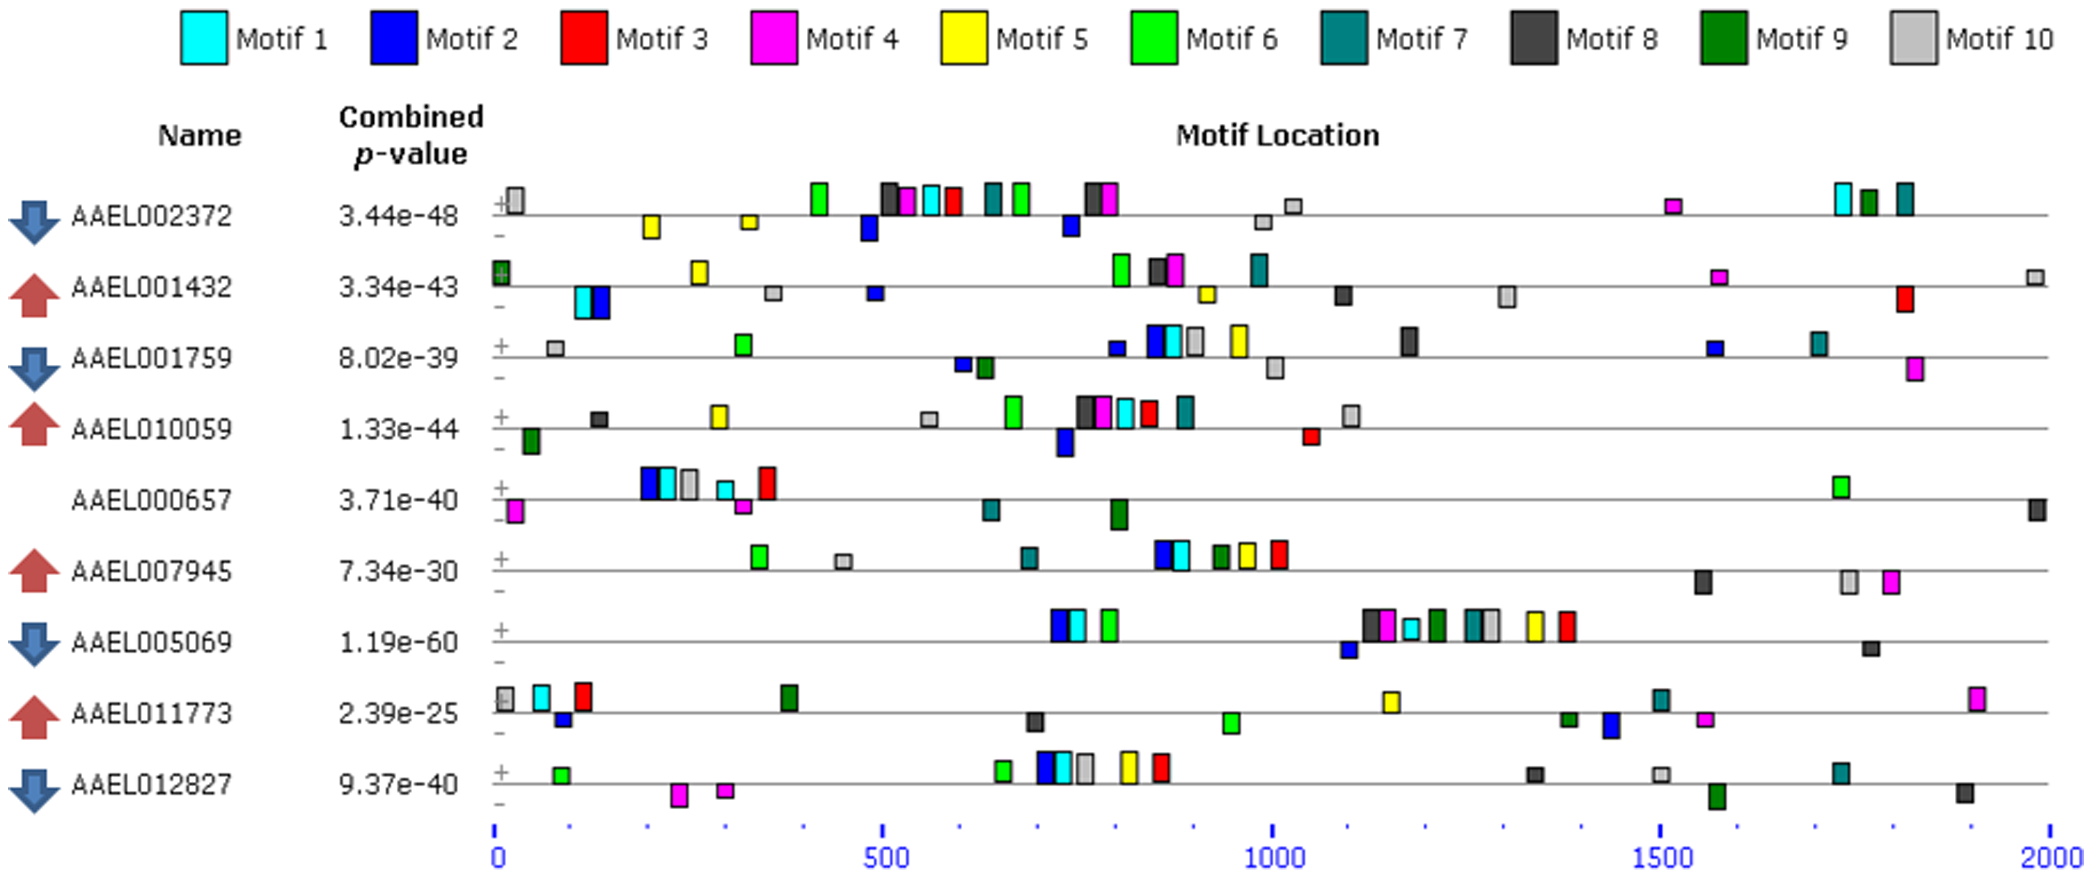
\includegraphics[width=.99\textwidth]{figures/figs/bonizzoni2012complex-cre.png}

\caption[MEME analysis of nine genes with \texorpdfstring{FPKM\textsubscript{DENVI}}{FPKM DENVI} ≥ 100 in carcasses and salivary glands at 14 dpi]{\sf \textbf{MEME analysis of nine genes with \texorpdfstring{FPKM\textsubscript{DENVI}}{FPKM DENVI} ≥ 100 in carcasses and salivary glands at 14 dpi} These genes also were identified with transcripts exhibiting significant differential accumulation in analyses of salivary gland samples of the Liverpool strain infected with DEV2 Thailand 16881 [26]. Colored boxes represent individual putative CREs and their locations in promoters of each gene. Red and blue arrows adjacent to Ensembl Gene ID indicate those genes whose transcripts were detected previously as more or less abundant following DENV infection [26]. Distances in base-pairs are provided below the schematic of each gene.
doi:10.1371/journal.pone.0050512.g004

Excerpted from \cite{bonizzoni2012complex}}
\label{fig:bonizzoni2012complex-cre}
\end{figure}

% \texorpdfstring{FPKM\textsubscript{DENVI}}{FPKM DENVI}

A total of 94 genes had FPKM ≥ 100 in \gls{DENVI} mosquitoes in both carcass and salivary gland samples at 14 \gls{dpi}, with corresponding values in B mosquitoes ≤ 100.
The putative promoter regions of these genes analyzed by MEME revealed the presence of two groups of motifs (Figure \ref{fig:bon2012complex-S5}: motifs 1, 2, 3, 4, 5, 7, 9, 10) co-occurring or alternating in 14 genes associated with diverse functions: AAEL001759 [40S ribosomal protein S9], AAEL005069 [ras-related protein Rab-1A], AAEL002372 [40S ribosomal protein S11], AAEL005165 [chaperone protein DNAj], AAEL000657 [hypothetical protein], AAEL005471 [Sec61 protein complex gamma subunit], AAEL001432 [protein disulfide isomerase], AAEL010059 [bacterial-type ABC transport ATP-binding subunit or RNAse l inhibitor], AAEL013407 [Catalase], AAEL007945 [eIF3 h], AAEL010169 [hypothetical protein], AAEL012827 [endoplasmin], AAEL011773 [calreticulin], AAEL010777 [TRX, putative].
These genes, except for AAEL002372, had high read coverage also in midgut samples, but not necessarily higher or equal accumulation in \gls{DENVI} versus B mosquitoes.
Some of these genes were detected previously as significantly differentially accumulated in the salivary glands of mosquitoes of the \gls{LVP} strain infected with \gls{DENV}2 Thailand 16681 (Figure \ref{fig:bonizzoni2012complex-cre}; \cite{Luplertlop2011}).
Specifically, the transcription products of AAEL001432, AAEL010059, AAEL007945 and AAEL011773 were more abundant in salivary glands of infected \gls{LVP}, while the opposite was observed for AAEL001759, AAEL005069, AAEL002372 and AAEL012827, which were more abundant in uninfected samples.
AAEL00657 was listed as both up- and down-regulated following \gls{DENV} infection, most likely at different time points, but this is not explicit in the report \cite{Luplertlop2011}.
MADS\_MCM1+SFF\_M01051 and bZIP transcription factors were the best matches to motifs 1, 2, 5 and 7 (e-value ≤ $10^{-5}$).
Motif 3 has sequence similarity with motifs 5 and 7 of the previously designated “carcass module” and matches to trp\_AtMYB-84\_M00970 (e-value = $2.25E-10$) and RREB-1 (e-value = $2.16E-7$).
The best match of motif 9 is to the HMG transcription factor ($1.87E-5$).


\subsection{Discussion}

The dengue-susceptible strain \gls{CTM} is well-documented in its ability to disseminate quickly viruses to peripheral tissues when compared to long-established laboratory strains \cite{Salazar2007}.
We describe in \citet{bonizzoni2012complex} changes in transcript accumulation levels in \gls{CTM} during the course of a Jam 1409 \gls{DENV}2 infection.
Our analyses include multiple post-infection time-points and three tissues important for the viral transmission cycle: midguts, salivary glands and carcasses, the latter of which includes the fat body.
The RNA-seq technology used in this study interrogates the whole \Aa\ transcriptome and allows for absolute quantification of poly-adenylated RNA levels.
In general, more depleted rather than enriched transcript accumulation was observed.
Importantly, hundreds of genes had exclusive read-coverage only in \gls{DENVI} mosquitoes, but their accumulation levels were generally low (FPKM$_{DENVI}$ < 4 in carcass and midgut samples and < 15 in salivary gland samples).

The “\gls{DENV} down-regulation” trend is consistent to that observed with the Rockefeller (ROCK) strain infected by \gls{DENV}2 New Guinea in transcriptional responses examined in whole-body (1–2, 7 and 14 \gls{dpi}) or midgut samples (10 \gls{dpi}) and in salivary glands of the \gls{LVP} strain infected with \gls{DENV}2 Thailand 16681 \cite{Xi2008}, \cite{Luplertlop2011}, \cite{Sim2012}, \cite{Colpitts2011}.
These results support the hypothesis that dengue infection has a negative impact on fitness.
However, a larger number of genes had products that increased instead of decreased in abundance in carcass samples 10 \gls{dpi} and in salivary glands at 14 \gls{dpi} in ROCK mosquitoes infected with \gls{DENV}2-New Guinea \cite{Xi2008}, \cite{Sim2012}.
This trend also was evident in \Aa\ Aag2 cultured cells infected by \gls{DENV}2 New Guinea and in both susceptible (Moyo-S) and resistant (Moyo-R) strains infected with \gls{DENV}2 Jam1409 \cite{Sim2010}, \cite{Behura2011}.
These results emphasize the complex relationship among \Aa\ and dengue viruses.



\subsubsection{\textit{Cis}-regulatory Elements}

The preferred promoter for an anti-dengue effector gene would be one that is induced following a bloodmeal and is not affected by viral infection.
Furthermore, we hypothesize that genes with this preferred expression profile may share common regulatory mechanisms based on common \glspl{CRE}.
Analysis of the 5′-end of genes whose transcripts exhibited accumulation profiles exclusively in salivary gland following \gls{DENV} infection did not reveal substantial co-occurrence of \glspl{CRE}.
The regulation of these genes is likely not coordinated through common promoter elements.
In contrast, co-occurring putative \glspl{CRE} were identified for genes whose transcripts were represented and modulated highly in response to dengue infection in midguts (1–4 \gls{dpi}), carcasses (all time points studied) and salivary glands and carcasses (14 \gls{dpi}).

Several of the identified motifs showed high-quality matches to known transcription factors.
The \glspl{CRE} likely are not related specifically to dengue infection since the majority of the genes included in the analyses also had read coverage in B mosquitoes.
This observation does not affect the potential utility of the \glspl{CRE} as components of synthetic promoters to direct expression of anti-dengue effector molecules.
Indeed, driving effector gene expression with control DNA that responds to an uninfected bloodmeal and either is unaffected or is enhanced by an infected bloodmeal could elicit a protective antiviral response in the mosquitoes.
Remarkably, 10 genes whose transcripts were modulated following \gls{DENV}2 16881 infection in \gls{LVP} salivary gland samples were among the 14 genes with FPKM$_{DENVI}$ ≥ 100 in our carcass and salivary gland samples that have a common group of \gls{CRE} motifs \cite{Luplertlop2011}.
However, not all of these ten genes had transcripts that were consistently more abundant following infection, and one gene, (AAEL00657), had transcripts reported as more and less abundant \cite{Luplertlop2011}.
These results and the findings that several motifs are putative binding sites for transcription factors acting through repressors and activators support a complex model of transcription modulation that requires further investigation.

\subsection{Conclusions}

Dengue fever is the most important arboviral disease world-wide, with \Aea\ being the major vector.
Interactions between the mosquito host and dengue viruses (\gls{DENV}) are complex and vector competence varies among geographically-distinct \Aa\ populations.
Additionally, dengue is caused by four antigenically-distinct viral serotypes (\gls{DENV}1–4), each with multiple genotypes.
Each virus genotype interacts differently with vertebrate and invertebrate hosts.
Analyses of alterations in mosquito transcriptional profiles during \gls{DENV} infection are expected to provide the basis for identifying networks of genes involved in responses to viruses and contribute to the molecular-genetic understanding of vector competence.
In addition, this knowledge is anticipated to support the development of novel disease-control strategies.
RNA-seq technology was used to assess genome-wide changes in transcript abundance at 1, 4 and 14 days following \gls{DENV}2 infection in carcasses, midguts and salivary glands of the \Aa\ Chetumal strain.
\gls{DENV}2 affected the expression of 397 \Aa\ genes, most of which were down-regulated by viral infection.
Differential accumulation of transcripts was mainly tissue- and time-specific.
Comparisons of our data with other published reports reveal conservation of functional classes, but limited concordance of specific mosquito genes responsive to \gls{DENV}2 infection.
These results indicate the necessity of additional studies of mosquito-\gls{DENV} interactions, specifically those focused on recently-derived mosquito strains with multiple dengue virus serotypes and genotypes.


The study of genome-wide changes in transcript abundance in \Aa\ following dengue infection is anticipated to identify genes and control DNA elements involved in vector competence.
This knowledge is expected to contribute to development of novel vector control strategies.
The interactions between the mosquito host and the virus are complex at both the individual and population levels.
Many mosquito tissues are affected by the virus during the course of the infection and \Aa\ strains can show unique responses of the transcriptome in response to a bloodmeal and susceptibility to \gls{DENV} infection \cite{Black2002}, \cite{bonizzoni2012strain}.
Additionally, the variation in \gls{DENV} serotypes and genotypes contributes to genetically-distinct differences in vector competence \cite{Anderson2006}, \cite{Weaver2009}.
While we identified modulations in transcript abundance following \gls{DENV} infection that represent genes encoding similar functional categories, a limited number of specific genes were concordant across the mosquito strains and \gls{DENV}2 genotypes following comparison of our data with previous studies \cite{Xi2008}, \cite{Luplertlop2011}, \cite{Behura2011}, \cite{Sim2012}, \cite{Colpitts2011}.
Furthermore, the direction of changes in transcript abundance in samples from infected and uninfected mosquitoes was not always conserved among the various studies, an observation that we consider independent of the methodology used to assess differential transcript accumulation.
These results support the need for a comprehensive analysis of dengue infection focusing on recently-colonized laboratory strains or wild-caught mosquitoes to capture most of the genetic variability at the host level and different \gls{DENV} serotypes/genotypes \cite{Armstrong2001}.
This analysis also should account for possible variation in the progression of the viral infection and timing of host gene expression.



\pagebreak
\section{Strain variation in the transcriptome of the dengue fever vector, \Aea. \cite{bonizzoni2012strain}}
%\todo[inline]{import text for STRAIN VARIATION}





Studies of transcriptome dynamics provide a basis for understanding functional elements of the genome and the complexity of gene regulation.
The dengue vector mosquito, \Aea, exhibits great adaptability to diverse ecological conditions, is phenotypically polymorphic, and shows variation in vectorial capacity to arboviruses.
Previous genome sequencing showed richness in repetitive DNA and transposable elements that can contribute to genome plasticity.
Population genetic studies revealed a varying degree of worldwide genetic polymorphism.
However, the extent of functional genetic polymorphism across strains is unknown.
The transcriptomes of three \Aa\ strains, \gls{CTM}, \gls{Rex-D} and \gls{LVP}, were compared.
\gls{CTM} is more susceptible than \gls{Rex-D} to infection by dengue virus serotype 2.
A total of 4188 transcripts exhibit either no or small variation (< 2-fold) among sugarfed samples of the three strains and between sugarfed and bloodfed samples within each strain, corresponding most likely to genes encoding products necessary for vital functions.
Transcripts enriched in bloodfed mosquitoes encode proteins associated with catalytic activities, molecular transport, metabolism of lipids, carbohydrates and amino acids, and functions related to blood digestion and the progression of the gonotropic cycle.
Significant qualitative and quantitative differences were found in individual transcripts among strains including differential representation of paralogous gene products.
The majority of immunity-associated transcripts decreased in accumulation after a bloodmeal and the results are discussed in relation to the different susceptibility of \gls{CTM} and \gls{Rex-D} mosquitoes to \gls{DENV2} infection.

This mosquito species is phenotypically polymorphic, has great adaptability to diverse ecological conditions, and shows variation in vectorial capacity for arboviruses \cite{Bennett2002,Black2002,Kuno2010}.
Genetic polymorphism among geographically distinct \Aa\ populations is documented \cite{Urdaneta-Marquez2011}; however, the extent of genome sequence polymorphism and its effects on transcriptional activity are not known.

The transcriptional profiles of three \Aa\ strains, \gls{LVP}, \gls{CTM}, \gls{Rex-D}, were investigated.
\gls{LVP} originated in West Africa in the 1930s, and its genome is sequenced \cite{Nene2007}, \gls{CTM} was derived from the Yucatan Peninsula in Mexico in the early 2000s \cite{Bennett2002,Gubler1985,Richardson2006a}, whereas \gls{Rex-D} was established from mosquitoes captured in Puerto Rico in the early 1990s \cite{Miller1991}.
\gls{CTM} supports a faster and more intense dissemination of \gls{DENV2} than \gls{Rex-D} \cite{Bennett2002,Salazar2007}.
Our data show significant differences in transcript accumulation among strains, and the results may account for the differing susceptibility of \gls{CTM} and \gls{Rex-D} mosquitoes to virus infection.


\subsection{Results}
\subsubsection{RNA-seq mapping summary}

Transcriptional profiles of \gls{LVP}, \gls{CTM}, and \gls{Rex-D} strains before and after a bloodmeal were compared.
RNA-seq libraries were generated with the use of RNA extracted from females collected 3 to 5 days after eclosion and kept either on a sugar diet (S) or harvested 5 h \gls{PBM} (B) (not shown).
Two RNA-seq libraries were constructed for each RNA sample.
The reproducibility of the parallel libraries was verified (not shown), and the data from the two technical replicates were merged for further analyses.
Reads mapping to multiple genomic locations were discarded during Bowtie alignment \cite{Langmead2009}.
As a consequence, the accumulation levels of transcripts encoded by highly conserved gene families are under-estimated.
This bias is expected to affect all samples equally; therefore, if the absolute accumulation level of a transcript is underestimated, differences across conditions still can be calculated.



\subsubsection{Constitutively accumulated transcripts}

A total of 4188 transcripts exhibit no or small variation (≤ 2-fold) among S samples of the three strains and between B and S samples within each strain and correspond most likely to genes that encode products necessary for vital and/or basal metabolic functions (not shown).
Function−parent attributions for this group of transcripts revealed a predominance of those encoding proteins with binding activity over transcripts with molecular function and catalytic activity (not shown).
Functional description is available for 2262 of these 4188 transcripts \cite{Lawson2009} (not shown).
More than 10 transcripts were found associated with each of the following classes: protein recycling (ubiquitin and proteasome), zinc finger proteins, WD-repeat proteins associated with diverse functions (i.e. RNA-processing complexes, transcription, cytoskeleton assembly), ribosome proteins, signal transduction (GTP binding proteins, G coupled proteins), redox processes (cytochrome), translation (eukaryotic translation initiation factor), transcription (transcription factors, mediator complex), membrane trafficking (rab), cell growth, differentiation and survival (ras), and immunity (PIWIs, autophagy proteins, galectins, TOLL, IMD, and JACK-STAT pathway signaling members).


Approximately 25\% of all analyzed transcripts accumulated differentially in S mosquitoes of different strains.
However, in the majority of cases the differences observed were lower than 2-fold (not shown).
Here is described only differences between the DEN-refractory \gls{Rex-D} and the more permissive \gls{CTM} strain.
Totals of 2992 and 2080 transcripts accumulated more in \gls{Rex-D} or \gls{CTM}, respectively.
Six were accumulated more than 5-fold in \gls{CTM} with respect to \gls{Rex-D}, including four of unknown function, one (AAEL005534-RA) annotated as a gonadotropin-inducible transcription factor, and one (AAEL014188-RA) annotated as a serine-type endopeptidase.
In contrast, 310 transcripts accumulated ≥ 5-fold in \gls{Rex-D} with respect to \gls{CTM}.
Functions could be attributed to 51\% of these and they include aldehyde oxidases, cytochrome P450s, G-coupled receptors, N-acetylgalactosaminyltransferases, and nicotinic acetylcholine receptors.
Immunity-associated transcripts accumulated differently in \gls{CTM} and \gls{Rex-D} S mosquitoes include five C-type lectins (AAEL008681-RA [CTL12], AAEL012353-RA [CTL15], AAEL005482-RA [CTL18], AAEL013566-RB [CTLGA2], AAEL017484-RA [CTLGA4]), two heme peroxidases (AAEL00376-RA [HPX4], AAEL002354-RA), one class B scavenger receptor (AAEL010655-RA [SCRBSP2]), a fibrinogen-related protein (AAEL008646-RA [FREP10]), and a Toll-like receptor (AAEL000671-RA [TOLL6]).


Quantitative reverse transcriptase, gene amplification, i.e., polymerase chain reaction (qRT-PCR) was performed on a selection of 13 transcripts and RNA from \gls{CTM}, \gls{Rex-D}, and \gls{LVP} mosquitoes.
The qRT-PCR results validated the RNA-seq data, with only two exceptions (transcript AAEL011871-RA in \gls{CTM} and AAEL008848-RA in \gls{Rex-D}; not shown).
To assess the similarity of the RNA-seq data with the qRT-PCR measurements, we calculated Pearson correlations of 0.97 (p < 0.001), 0.85 (p < 0.001), and 0.90 (p < 0.01) for \gls{LVP}, \gls{CTM}, and \gls{Rex-D}, respectively.
T-test values were 2.18 (p = 0.148), 2.18 (p = 0.453), and 2.18 (p = 0.188), respectively, for the three strains (not shown).

The accumulation of 1845 and 981 transcripts consistently increased and decreased, respectively, in all three strains after a bloodmeal (not shown).
In general, \gls{Rex-D} exhibited the lowest fold-changes and the smallest number of transcripts accumulated highly after the bloodmeal (not shown).
This observation supports the interpretation that \gls{CTM} mosquitoes respond quicker or more intensively to a bloodmeal than \gls{LVP} and \gls{Rex-D}.
To test this hypothesis, the expression profiles of five transcripts were analyzed by qRT-PCR at 5, 8, 12, and 24 h \gls{PBM}.
Results for four of the five transcripts tested showed a greater response of \gls{CTM} to a bloodmeal compared with mosquitoes of the other two strains (not shown).




Despite the observation that the same functional classes are represented within groups of transcripts that increased and decreased in accumulation after a bloodmeal, the numbers of transcripts associated with the various functions differed significantly (not shown).
The transcripts accumulated after a bloodmeal were enriched in functions related to protein-turnover and chaperones, transcription, translation, posttranslational modification, and RNA processing.
These transcripts encode proteins associated with catalytic activities, in transport and metabolism of lipids, carbohydrates and amino acids, and related to blood digestion and the progression of the gonotropic cycle.
Many of the transcripts showing the greatest decrease in accumulation after a bloodmeal in all three strains encode structural proteins.

The number of strain-specific transcripts varying highly (< 10-fold) in abundance between B and S mosquitoes is smaller in general than those found in all three strains (not shown).
\gls{CTM} mosquitoes show both the greatest number of strain-specific, differentially accumulated transcripts (not shown) and the largest range of changes in transcript accumulation levels.
Overall, the largest proportion of transcripts showing strain-specific increased accumulation after bloodmeal are linked to binding and catalytic functions and associated with transcription, translation, and posttranslational modification, whereas the largest proportion of strain-specific decreased transcripts are linked to transcription, translation, posttranscriptional modification, and RNA processing in \gls{LVP} and \gls{CTM} and to transport and metabolism of lipids, carbohydrates, and amino acids in \gls{Rex-D} (not shown).


\subsubsection{Protein network analysis of bloodmeal-induced changes in transcript accumulation}

By using a Markov Cluster algorithm, \cite{Guo2010} developed a protein interaction network in which 3500 \Aa\ proteins are organized into 494 functional modules.
A total of 2465 of these proteins are encoded by transcripts exhibiting significant differential accumulation between B and S mosquitoes in at least one of the three strains analyzed (not shown).
Modules enriched in Gene Ontology terms for cytoplasm organization and biogenesis, ribosome biogenesis and assembly, transcription, DNA metabolic processes, response to endogenous stimuli, and cell cycle were enriched significantly with proteins encoded by transcripts increased in accumulation in all three strains after a bloodmeal (not shown).
A module enriched in Gene Ontology terms for cytoskeleton organization and biogenesis, reproduction, and cell differentiation was enriched significantly with proteins corresponding to transcripts consistently decreased in accumulation following a bloodmeal.
Results from the protein network analyses are consistent with those from functional attribution of the differentially accumulated transcripts.

\subsubsection{Metabolic pathways involving transcripts differentially accumulated post-bloodmeal}

\begin{figure}[h]

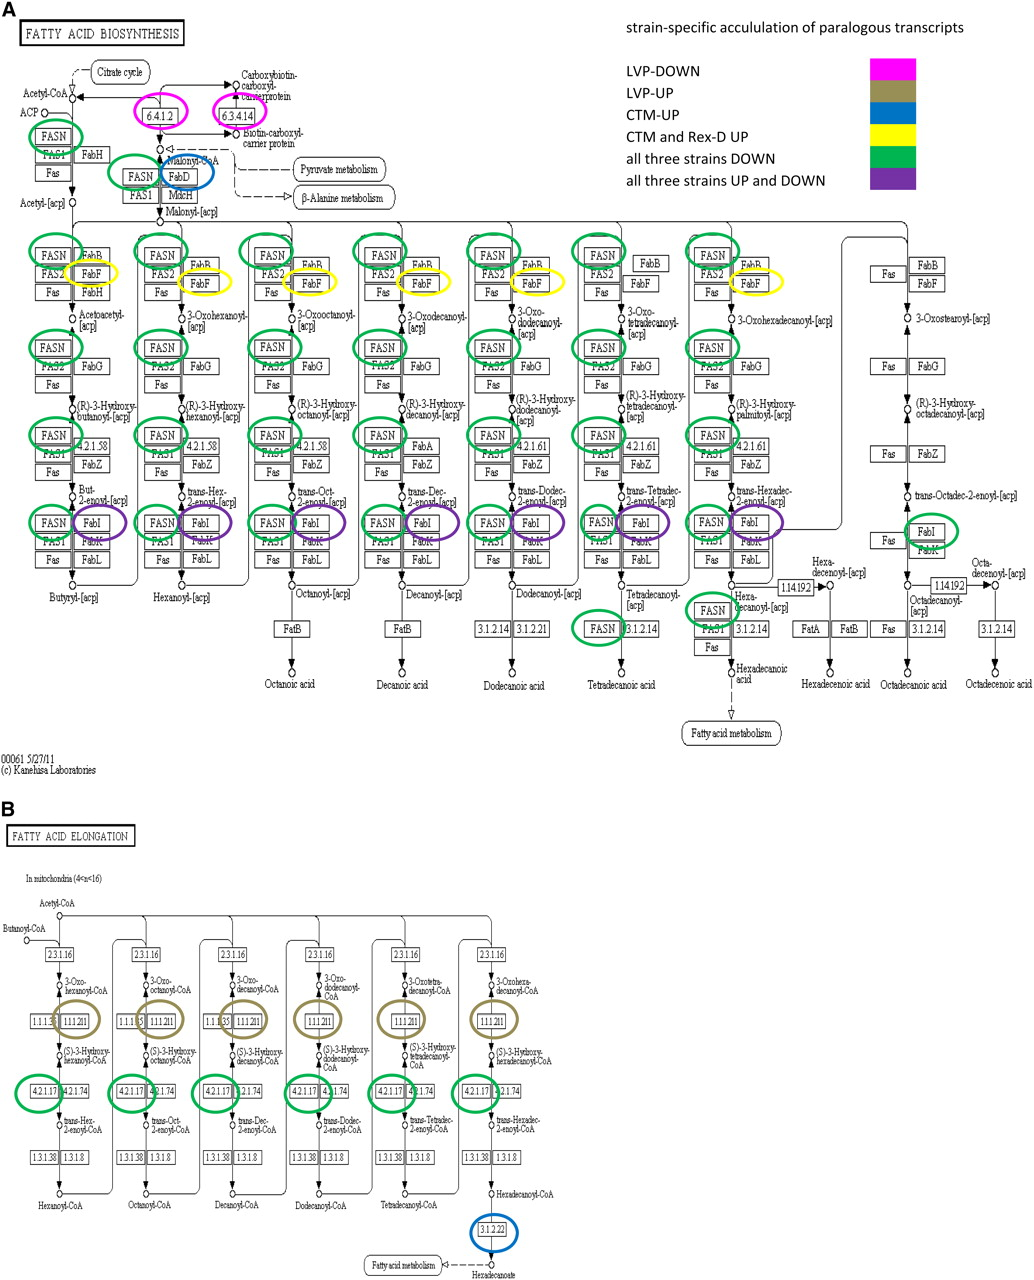
\includegraphics[width=.9\textwidth]{figures/figs/aa-diff-paralogs.jpg}

\caption[Fatty acid biosynthesis and elongation in mitochondria]{\sf \textbf{Fatty acid biosynthesis and elongation in mitochondria:} Proteins corresponding to transcripts accumulated in a strain-specific manner are circled in a color corresponding to the strain and condition defined in the legend (panels A and B).

Excerpted from \cite{bonizzoni2012strain}}
\label{fig:aa-diff-paralogs}
\end{figure}

Metabolic pathways correlated with transcripts increased in accumulation after a bloodmeal in all three strains were visualized in LinkinPath \cite{Ingsriswang2011} alongside pathways associated with transcripts accumulated in a strain-specific manner and transcripts decreased in accumulation after a bloodmeal (not shown).
As seen with the function−parent attribution analyses, the transcripts increased and decreased in accumulation are associated with proteins involved in similar pathways.
However, differential expression of paralogous genes among the strains was observed that could account for the intensity and/or the rate of pathway activation/deactivation after a bloodmeal.
For example, biosynthesis of fatty acids associates predominantly with transcripts decreased in accumulation in all three strains after a bloodmeal, but the elongation of fatty acids in mitochondria was exclusively associated with transcripts increased in accumulation (Figure \ref{fig:aa-diff-paralogs}).
Proteins corresponding to transcripts accumulated differentially in a strain-specific manner were identified in both cases, with the same protein function encoded by paralogous transcripts in the different strains.
Examples include FabI (enoyl-[acyl carrier protein] reductase) of the fatty acid biosynthesis pathway linked to transcripts AAEL003961-RA and AAEL002493-RA, which significantly increased in all three strains (fold-changes: 1.4-2.4); AAEL009634-RC and AAEL014840-RA, both of which increased 2-fold in \gls{CTM}; AAEL000705-RA, AAEL000689-RA and AAEL004273-RA, which decreased in \gls{CTM} (fold-changes: 2.5-4.4); AAEL009685-RB, which decreased 5.4-fold in \gls{Rex-D}; and AAEL017302-RA, AAEL007669-RA, AAEL008227-RA, AAEL009625-RA, AAEL013491-RA, AAEL017320-RA, AAEL000690-RA, AAEL002228-RA, AAEL003148-RA, AAEL003183-RA, AAEL010075-RA, AAEL012400-RA, and AAEL008016-RA, which decreased in all three strains, with fold-changes in the range of 0.6-11.3.
All of these transcripts are annotated currently as short-chain and steroid dehydrogenases, oxidoreductases, or fatty acid synthases \cite{Ribeiro-AegyXcel} and match to short-chain dehydrogenases in the PFAM database \cite{Finn2008}, with the exception of AAEL002228-RA, whose best match is ketoacyl synthase.
They all have the PKS\_KR enzymatic domain as a best match in the SMART database \cite{Letunic2009}, except for AAEL012400-RA, which matches the SEP enzymatic domain.
The protein HADHA (4.2.1.17 in the fatty acid elongation pathway), functioning as an aldehyde reductase and enoyl-coA hydratase, is associated with transcripts AAEL010146-RB (annotated as 3-hydroxyacyl-coa dehydrogenase) and increased 2.9-fold in \gls{LVP} and AAEL003993-RA (putative cyclohex-1-ene-1-carboxyl-CoA hydratase), which increased in all three strains with fold-changes ranging between 1.6 and 2.3.


Another example of differential accumulation of transcripts representing paralogous genes is seen in the lipase gene family.
Three genes (AAEL001837, AAEL007055, AAEL14551) of the 72 annotated currently as lipases correspond to transcripts accumulated differentially after a bloodmeal in all three strains (fold-changes: −7.5 to 4.3) and eight to transcripts accumulated differentially in a strain-specific manner.
Two (AAEL002909-RA, AAEL001076-RA) of these latter transcripts were found exclusively in S and one (AAEL006970-RA) only in B \gls{CTM} mosquitoes.
The remaining had fold-changes ranging from −2.2 to 2.6.
No reads were mapped in any sample for 21 lipase genes, which may indicate that they are expressed exclusively in adult males or during pre-adult stages of \Aa\ development.
Alternatively, these predicted genes could be pseudogenes.



\subsection{Discussion}
The results reported here reveal that the transcriptomes of \Aa\ mosquitoes from distinct strains vary significantly in complexity and abundance of specific transcripts.
This variation is evident in non-bloodfed mosquitoes and is enhanced after a bloodmeal.
\gls{CTM} showed a larger number of differentially abundant transcripts after a bloodmeal and a wider range of fold-changes than \gls{Rex-D} and \gls{LVP}.


Transcripts associated with metabolism and transport of lipids, carbohydrate and amino acids, and the progression of the gonotropic cycles were among the most increased in accumulation after bloodmeal.
Transcripts decreased most in accumulation after a bloodmeal are associated with structural components.
Transcripts attributed functions in transcription, translation, and posttranslational protein modification also were highly differentially-accumulated, but many of these show strain-specific regulation.
These observations support the hypothesis that important differences among the strains are conferred by distinct patterns of gene expression, protein synthesis and modifications.
Strain differences also may result from selective expression of paralogous transcripts.


Digestion and immunity share bio-products such as \gls{ROS} \cite{Molina-Cruz2008}, and these processes are linked at the protein network level \cite{Guo2010}.
The majority of immunity-related genes were decreased in accumulation in all three strains after a bloodmeal.
The most pronounced decrease in accumulation was observed for the antimicrobial peptide \gls{AMP} (AAEL003389-RA).
Indeed, all AMPs decreased in accumulation with the exception of CecF (AAEL000625-RA), which significantly increased in accumulation exclusively in \gls{CTM}.
The overall AMP decrease may be associated with an increase in bacterial proliferation observed after a bloodmeal \cite{Oliveira2011}.
The most common midgut bacteria do not show proteolysis activity but are implicated in the lysis of red blood cells, which release hemoglobin \cite{Gaio2011}.
At the same time, hemoglobin negatively affects ROS production in the midgut, which triggers bacteria proliferation \cite{Oliveira2011}.
Although ROS reduction potentially favors DEN infection \cite{Oliveira2011}, bacteria proliferation antagonizes it \cite{Xi2008}.
Antioxidant activity by peroxidase and superoxide-dismutase varied across strains.
\gls{CTM} showed the greatest number of transcripts associated with antioxidant activity accumulated after a bloodmeal among the strains analyzed.
In addition, S \gls{CTM} mosquitoes accumulate greater levels of transcripts associated with antioxidant activity than \gls{Rex-D}.
\gls{CTM} also had the largest number of P450 and glutathione-s transferase transcripts accumulated differentially after a bloodmeal, with increases in accumulation up to 15-fold (AAEL000325-RA).
These results support a model of more intense antioxidant activity in B \gls{CTM} than in \gls{Rex-D}, which may facilitate DENV infection in the former.

Transcripts encoding proteins associated with autophagy, IAPs, IMD pathway, and SRRP members represent immunity genes that showed an exception to the overall decline in corresponding-transcript accumulation after a bloodmeal.
Increases were overall within 2-fold.
A notable exception is the IMD pathway member Caspar1 (AAEL014734-RA) that increased 4.7- to 5.8-fold in all strains.
Caspar is a negative regulator of the IMD pathway \cite{Kim2006caspar}; therefore, its up-regulation is consistent with the observed decrease in accumulation of AMPs.

In summary, the \Aa\ strains analyzed demonstrated variability in their transcriptomes before and after bloodmeal.
Profiles differ in the number of transcripts detected, their level of accumulation in S mosquitoes, and in the changes in accumulation following the ingestion of a bloodmeal.
Although these differences may result from distinct RNA turnover rates among strains, it is most likely a result of differential gene regulation.
These data indicate the need for caution in making generalizations about individual gene expression profiles across different strains of \Aa.
For example, constructs used in genetics-based strategies of vector control would require the previous analyses of cross-strain promoter activity \cite{James2011}.
The differences observed encompass several transcripts associated previously with vectorial capacity to DENV.
Future studies will investigate the transcriptomes of \gls{CTM} and \gls{Rex-D} mosquitoes infected with \gls{DENV2}.
Also, it will be necessary to assess the susceptibility of \gls{CTM} and \gls{Rex-D} to other DENV serotypes to determine whether or how their distinct transcriptional responses to bloodmeals described herein influence vector competence.




%%% Local Variables: ***
%%% mode: latex ***
%%% TeX-master: "thesis.tex" ***
%%% End: ***

% Figure / table inputs

\chapter{Approach and Custom Software solutions} \label{chap:3}
\todo[inline]{replace CITEME tags in Approach and Custom Software solutions}


Frequently, \gls{functional-genomics} approaches contain problems or subproblems that require generating biologically meaningful gene-sets that pertain to the focus of the particular phenomenon being targeted.
Optimizing signal-to-noise ratios in data is a major challenge to generating useful gene-sets.
This project aims to generate meaningful gene-sets through integrating information from four supporting data-types:

\begin{itemize}
    \item comparative genomics ($N$-way 1-to-1 ortholog relationships)
    \item comparative transcriptomics (identical \gls{RNA-Seq} experiments performed using divergent mosquito species with the shared trait of \gls{hematophagy})
    \item phylogenetics (estimated divergence since last common ancestor)
    \item putative regulatory mechanisms (predicted \gls{TFBS} profiles)
\end{itemize}



\section{Preliminary data preparation} \label{sec:prelim-data}

Four foundational data-sets were compiled that represent Genomics, Transcriptomics, Phylogenetics, and Putative Transcriptional Regulatory information.

\paragraph*{Comparative Genomics:}

The initial gene-set for this project was limited to genes that have exactly one matching 1-to-1 ortholog in \Aa, \Ag, \As, and \Cq.
The purpose of this constraint is to maximize the probability of conserved function between genes analyzed. 

This preliminary gene set was obtained using the orthoDB7 \url{http://cegg.unige.ch/orthodb7} website by first selecting the node representing only the mosquito branch of the phylogeny \cite{Waterhouse2013}.
Then, the following requirements were enforced when retrieving ortholog relationship results 

\begin{quotation}
    \texttt{co-ortholog copy-number: AAEGY=1, AGAMB=1, ASTEP=1, CQUIN=1}
\end{quotation}


\begin{landscape}

\begin{figure}[hp]
\centering
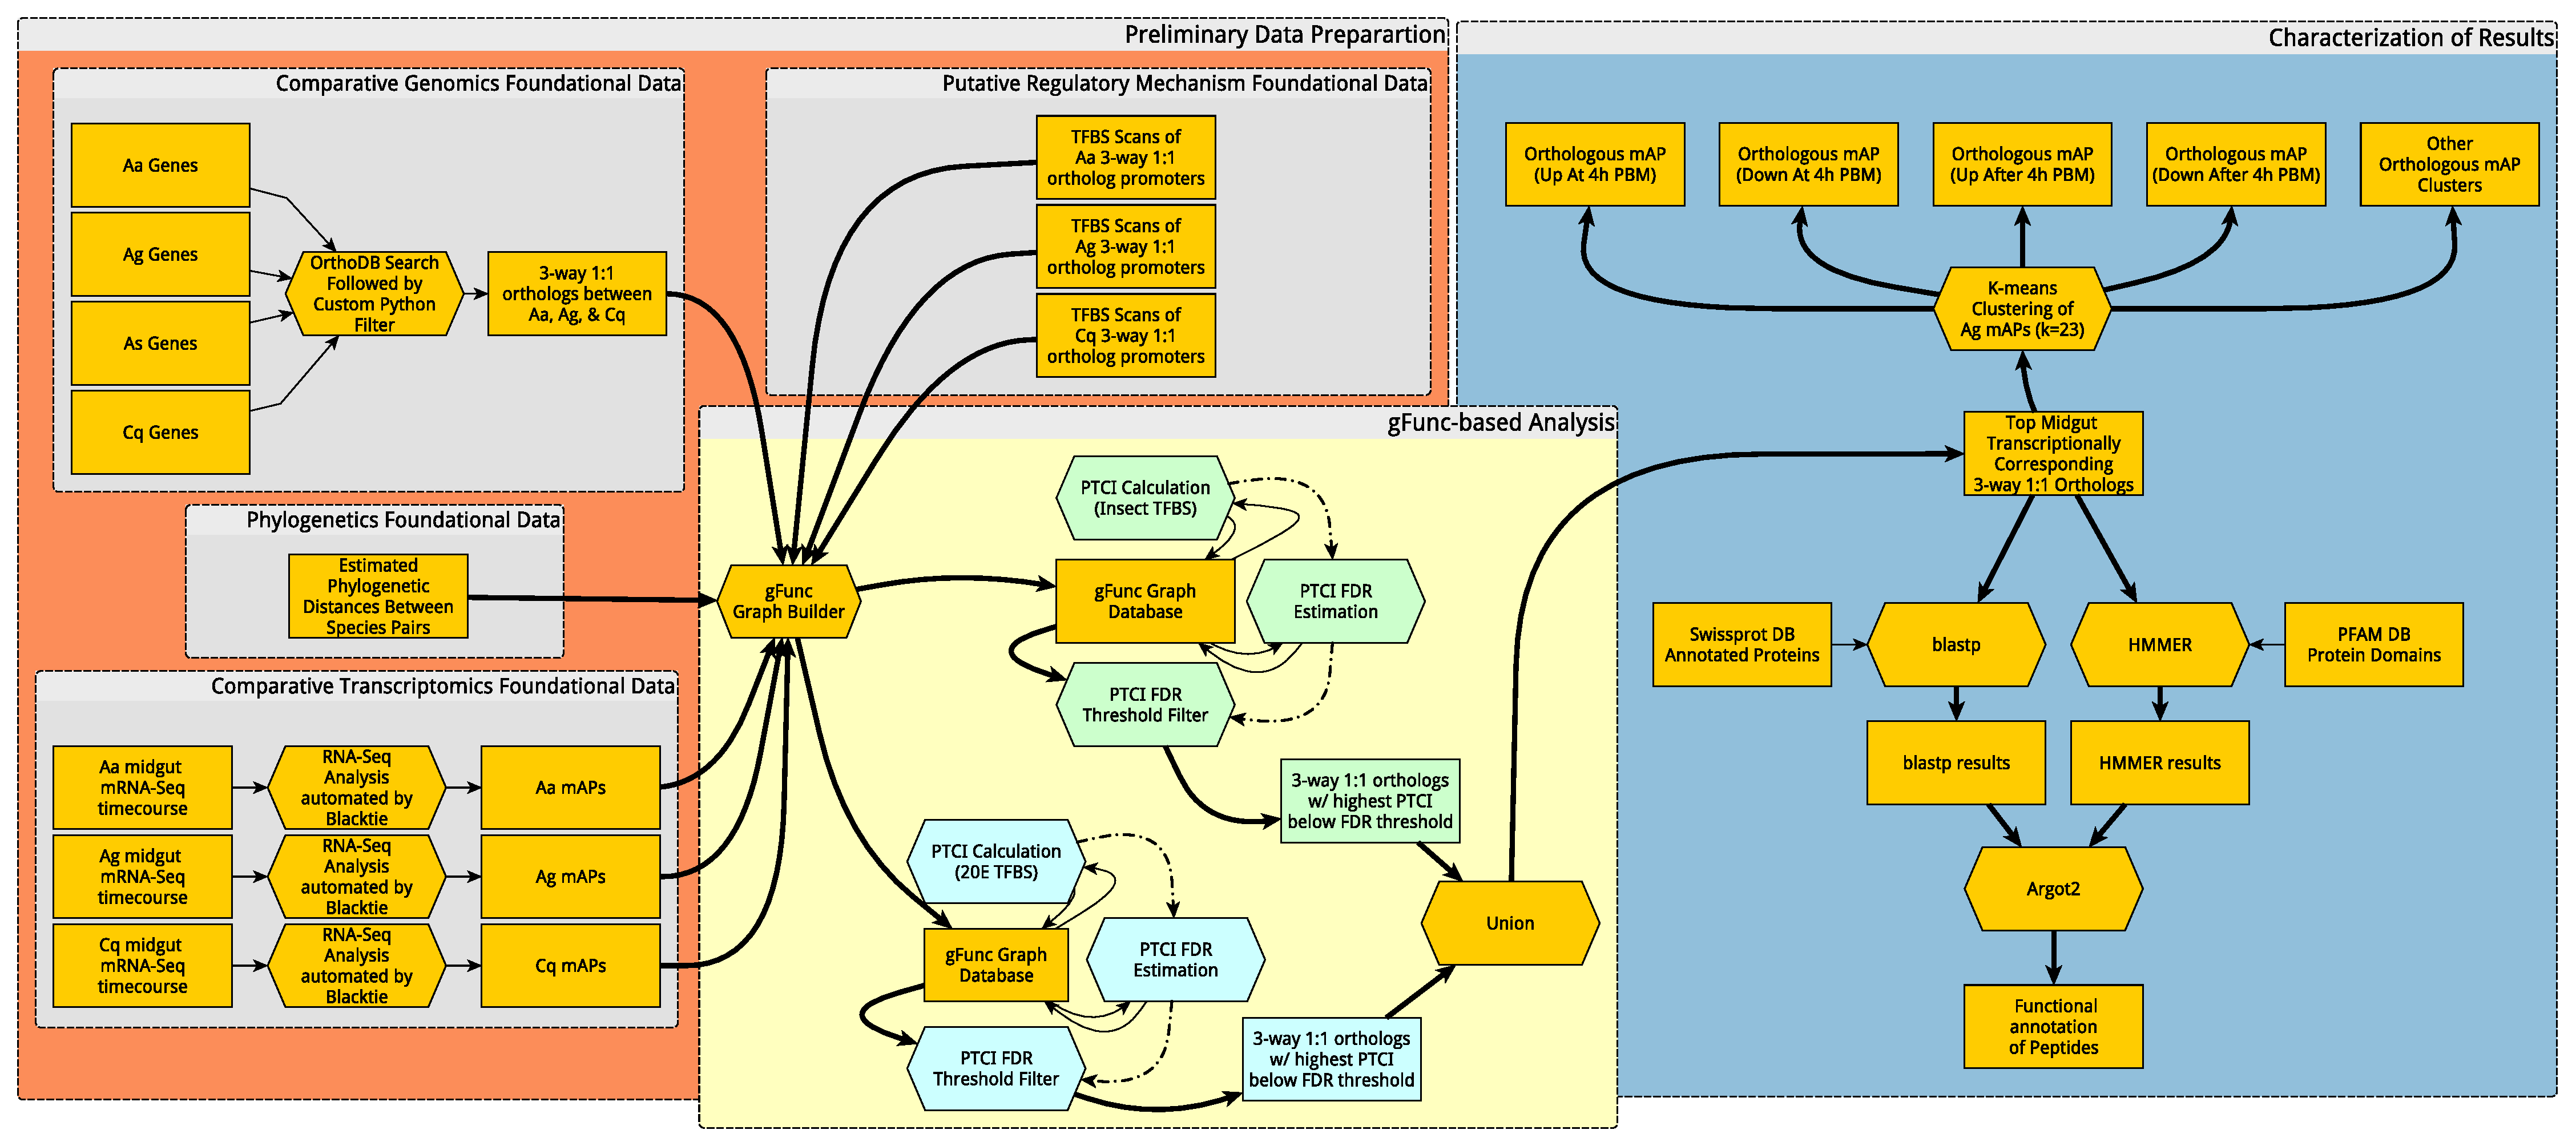
\includegraphics[width=\linewidth]{figures/figs/approach_chart/approach_overview.pdf}

\caption[Input-output diagram of approach overview]{
\sf \textbf{Input-output diagram of approach overview:}
%
The approach employed can be divided into three stages.
\emph{Preliminary Data Preparation }consists of accumulating and preparing the foundational data representing the four data-types to be integrated into the \gls{gFunc} graph.
\emph{gFunc-based Analysis} involves mapping the foundational data onto the gFunc graph structure and submitting the graph to custom Python functions that read, analyze, and write results back to the graph to calculate the \glspl{PTCI} and corresponding \glspl{FDR}.
This is done using two \gls{TFBS} profile data-sets with results being merged by a union-type set-operation to obtain the overall set orthologs representing putatively conserved midgut \glspl{mAP}.
\emph{Characterization of Results} then uses \gls{Argot2} \cite{Falda2012} to obtain functional annotations of the ortholog-sets, and the \glspl{mAP} of \Ag\ members are clustered using k-means clustering to group the ortholog-sets by expression similarity.


\emph{Heavy Arrows:} main flow of data;
\emph{Light Arrows:} preliminary or minor data flow;
\emph{Dashed Arrows:} establishes the order of execution;
\emph{Square Node:} data set;
\emph{Hexagon Node:} analysis operation.

}
\label{fig:approach-chart}
\end{figure}

\end{landscape}

The results of the query are provided as file \texttt{orthodb7\_mosqs\_20130918.txt} in the supplementary data files associated with this dissertation \cite{Dunn2013dissSupl}.
 
Custom python code was used to extract the 1-to-1 orthologs for \Aa, \Ag, and \Cq\ (Figure \ref{fig:approach-chart}).
The coded process is provided as an executable IPython notebook located at \url{http://goo.gl/EM1pHL} for in-depth inspection as well as for the purpose of openness and reproducibility.

Briefly, the results table was filtered for data pertaining to \Aa, \Ag, or \Cq.
Then I built a graph-representation of the data such that each orthoDB ortholog group could be queried to ensure that exactly one gene was represented for each species of interest.
These genes represent gene-set that formed the starting point for the rest of my approach.
The filtered set is available as supplementary file \texttt{AaAgCq\_1to1\_orthos.tsv} \cite{Dunn2013dissSupl}.

It should be noted that while this set contains only genes from the three species included in this document, each group should also have exactly one ortholog from \As\ as well which represents an additional constraint intended to limit the ortholog-sets to those most likely to fulfill the same function in each species.

\paragraph*{Comparative Transcriptomics:}

Whole RNA was extracted from dissected midguts of 16 female individuals of each species among the following time points: \gls{NBF} (0), 2, 4, 6, 8, 10 h \gls{PBM} (Protocol \ref{prot:RNA_Judy}) to identify and analyze orthologous genes that exhibit correlated \glspl{mAP} in the midguts of females directly following the ingestion of a bloodmeal.


\paragraph*{Phylogenetics:}

The phylogenetics aspect of this approach consists of using the estimated phylogenetic distances between each species to weight the comparisons between data correlations calculated for each pairwise 1-to-1 ortholog duo.
This is encoded as $d$ in the \gls{PTCI} expression defined in Equation \ref{eq:ptci} (see Section \ref{sec:ptci}).

The values of $d$ for each species-pair have been estimated previously (Table \ref{tab:evo-ranges}) (compiled in \citet{Sieglaff2009}).


\begin{table}[h]
\centering \sffamily
{%
\newcommand{\mc}[3]{\multicolumn{#1}{#2}{#3}}
\begin{center}
\begin{tabular}{llc}\toprule
\mc{2}{c}{\textbf{Species Pair}} & \textbf{Mya}\\ 
\midrule
\Aa & \Ag & 145\\
\Ag & \Cq & 145\\
\Aa & \Cq & 22\\ \bottomrule
    \end{tabular}
    \end{center}
}%

\caption[Estimated pairwise-evolutionary divergence between species]{\bsf{Estimated pairwise-evolutionary divergence between species}}
\label{tab:evo-ranges}
\end{table} 



% 
%     \Aa \Ag = 145 MYA 
%     \Ag \Cq = 145 MYA 
%     \Aa \Cq = 22 MYA  
%     




\paragraph*{Putative Transcriptional Regulatory Control Mechanisms:}

Part of the \gls{PTCI} includes correlation of a \gls{TFBS} scanning signature between ortholog pairs.
If the \gls{PTCI} is calculated using a set of \gls{TFBS} that are known to interact with the \gls{20E} signaling cascade, then this portion of the \gls{PTCI} acts as a rough proxy for correlation with putative activity of the \gls{20E} cascade.

The \gls{TFBS} profiles are obtained through scanning the 2000 bp regions 5' to the annotated start of transcription for each gene using the \gls{MOODS} application wrapped in custom Python code \cite{Pizzi2009}.
The scoring method used was log-odds.
The final \gls{TFBS} profile score for a gene-motif combination consists of the sum of all site-scores with positive log-odds scores.
In this way the gene-motif score represents the count of all site-scores that fit the motif model better than would be expected after considering the background sequence-composition of the putative promoter-regions weighted by the log-odds value of each site-score.
For example, for motif model $m$, if one sequence had three sites that each received log-odds scores of 0.33, then the gene-motif score is approximately 1.
Alternatively, if a second sequence has a single site that matches $m$ with a positive score of 1, both sequences would have approximately equal gene-motif scores for $m$.
Just as the \gls{mAP} for a particular gene consists of 5 values that represent the \gls{FPKM} score for that gene at 5 time-points, the \gls{TFBS} profile of a gene consists of $N$ values (the number of motif models considered) that represent the sum of sites in the putative promoter region that received a positive log-odds value weighted by the log-odds value of each site.

This is an imperfect solution as \gls{ChIP-Seq} using antibodies to specific \glspl{TF} in each species is preferable\footnote{those that are presently associated with \gls{20E} for instance}.
However this was impractical for this work due to the absence of suitable antibodies and the cost of developing and executing all assays in each species.


\section{The phylogenetic transcriptional correspondence index (PTCI)} \label{sec:ptci}

The \gls{PTCI} (Equation \ref{eq:ptci}) attempts to provide a metric that combines multiple pairwise \glspl{Pcc} ($r$) relating to multiple comparison dimensions for each 1:1 ortholog-pair then weight it by the relative evolutionary divergence times of each pairwise comparison ($d$).
%


\begin{equation} \label{eq:ptci}
PTCI = ( r_{x} + \frac{r_{t}}{2} ) \cdot w(d)
\end{equation}

%
In Equation \ref{eq:ptci}, the two comparison dimensions being combined are the similarity between an ortholog-pair with respect to \gls{mAP} ($r_{x}$) and \gls{TFBS} profile signature ($r_{t}$).
The pairwise species-divergence is represented by $d$.
However, the divergence times must be scaled using function $w()$ that prevents the \textbf{much} larger values of raw divergence values from dominating the index.
I have chosen to constrain the range of $w(d)$ between $1$ (no reward) and $1.1$ (a reward of 10\%).
This range was chosen to allow the evolutionary distance to affect the ranking of an ortholog-set without having a dominating effect.
I explored other constraint settings, but this range appeared to be a good compromise (not shown).%
%




\begin{figure}[hp]
\centering
  \begin{subfigure}[b]{.9\linewidth}
    \centering

    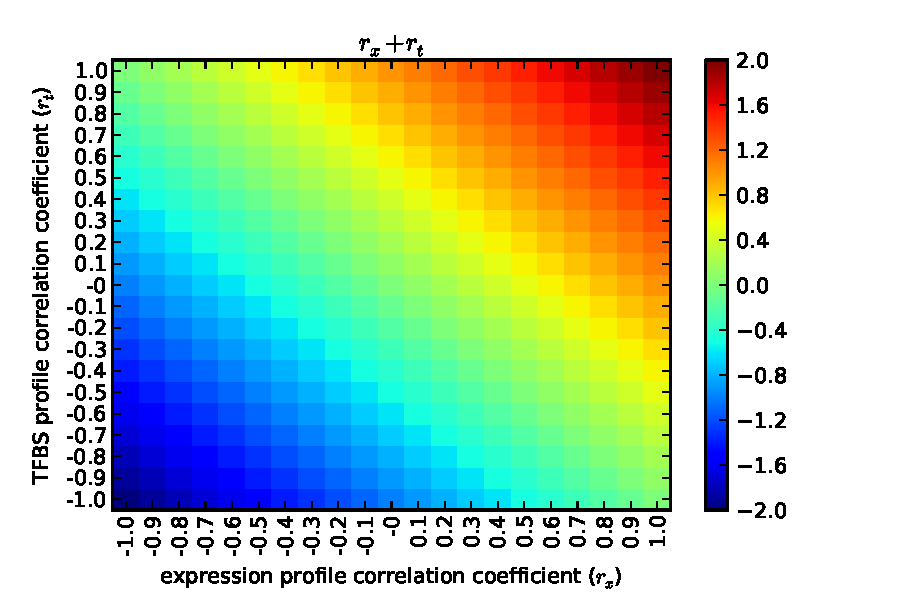
\includegraphics[width=.9\linewidth]{figures/figs/thesis-xprn-tfbs.pdf}
    \caption{}
    \label{fig:ptci-space-a}
  \end{subfigure}%

  

  \begin{subfigure}[b]{.9\linewidth}
    \centering

    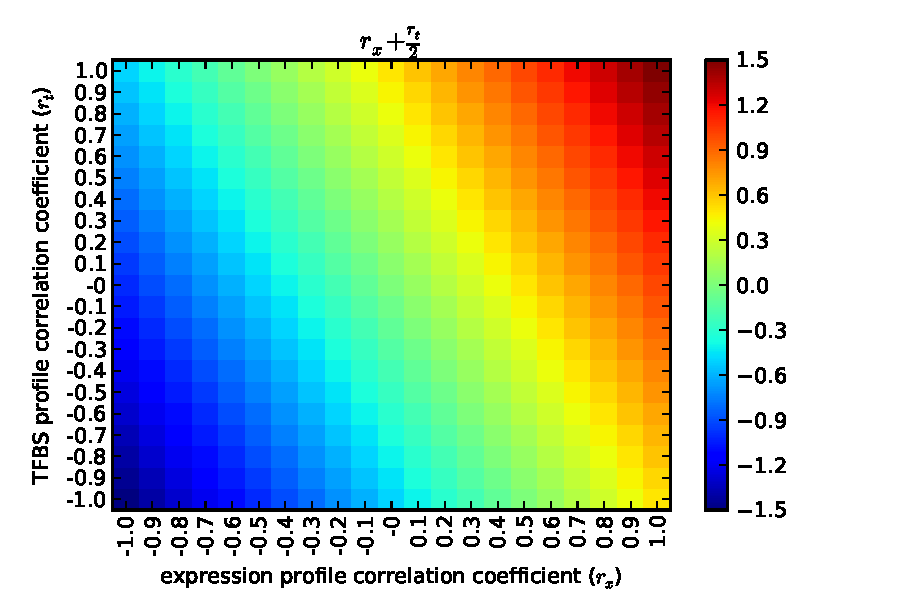
\includegraphics[width=.9\linewidth]{figures/figs/thesis-xprn-scaled-tfbs.pdf}
    \caption{}
    \label{fig:ptci-space-b}
  \end{subfigure}

\caption[Exploring the parameter space of the expression and TFBS components of the PTCI]{\sf \textbf{Exploring the parameter space of the expression and TFBS components of the PTCI:} \\
\textbf{(A)} The expression and TFBS profile correlations each carry the same weight.  TFBS data is not strictly empirical, and position weight matrix models inherently are prone to produce false positive predictions. Here, each correlation-type exerts equal influence on the final score assigned to the ortholog relationship.  \textbf{(B)} The TFBS profile correlation is penalized due to the non-empirical nature and expected false positive information it contains. Here, TFBS profile data contributes to the final score at most 50\% as much as expression data.}
\label{fig:ptci-space}
\end{figure}%
%
The \gls{TFBS} data is derived through imperfect and non-empirical means\footnote{They are non-empirical in that they are statistical predictions rather than the results of physical experiments.}.
Therefore, they should not carry the same significance as the information encoded in the \glspl{mAP}.
I explored several methods for combining the two correlations.
Equation \ref{eq:ptci} values the \gls{TFBS} correlations at 50\% of the \gls{mAP} correlations.
This avoids scenarios in which an ortholog-pair that has $r_{x} = 0$ and $r_{t}=1$ ranks the same as if the values were opposite while still allowing the \gls{PTCI} to be positive overall\footnote{Positive \gls{PTCI} implies positive combined correspondence between the ortholog correlations which may still be valid even with the failure to detect correlation between \glspl{mAP} when combined with the detection of very strong correlation between \gls{TFBS} profiles.} but rank below ortholog-pairs with $r_{x} = 1$ and $r_{t}=0$ (Figure \ref{fig:ptci-space}).
Figure \ref{fig:ptci-space} provides detailed illustrations of the effects of weighting the \gls{TFBS} information at 50\% of the \gls{mAP} data across the spectrum of possible $r_{x}$ and $r_{t}$ value-combinations.


\begin{figure}[hp]
\centering
% 
    \begin{subfigure}[t]{.5\linewidth}
    \centering
    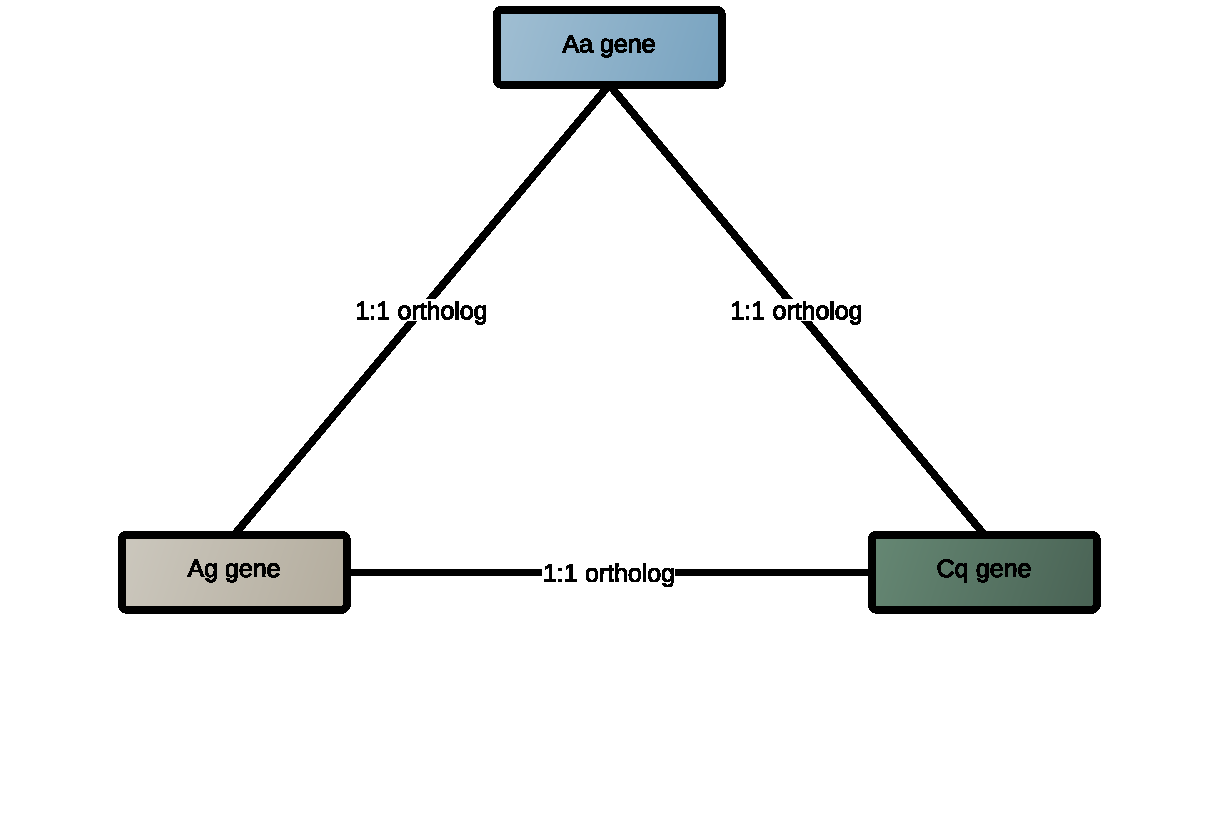
\includegraphics[width=\linewidth]{figures/figs/gfunc_graph_figs/ortho-graph-model.pdf}
    \caption{N-way 1:1 ortholog graph structure}\label{fig:nway-ortholog-graph-model}
    \end{subfigure}%
% 
% 
% 
    \begin{subfigure}[t]{.5\linewidth}
    \centering
    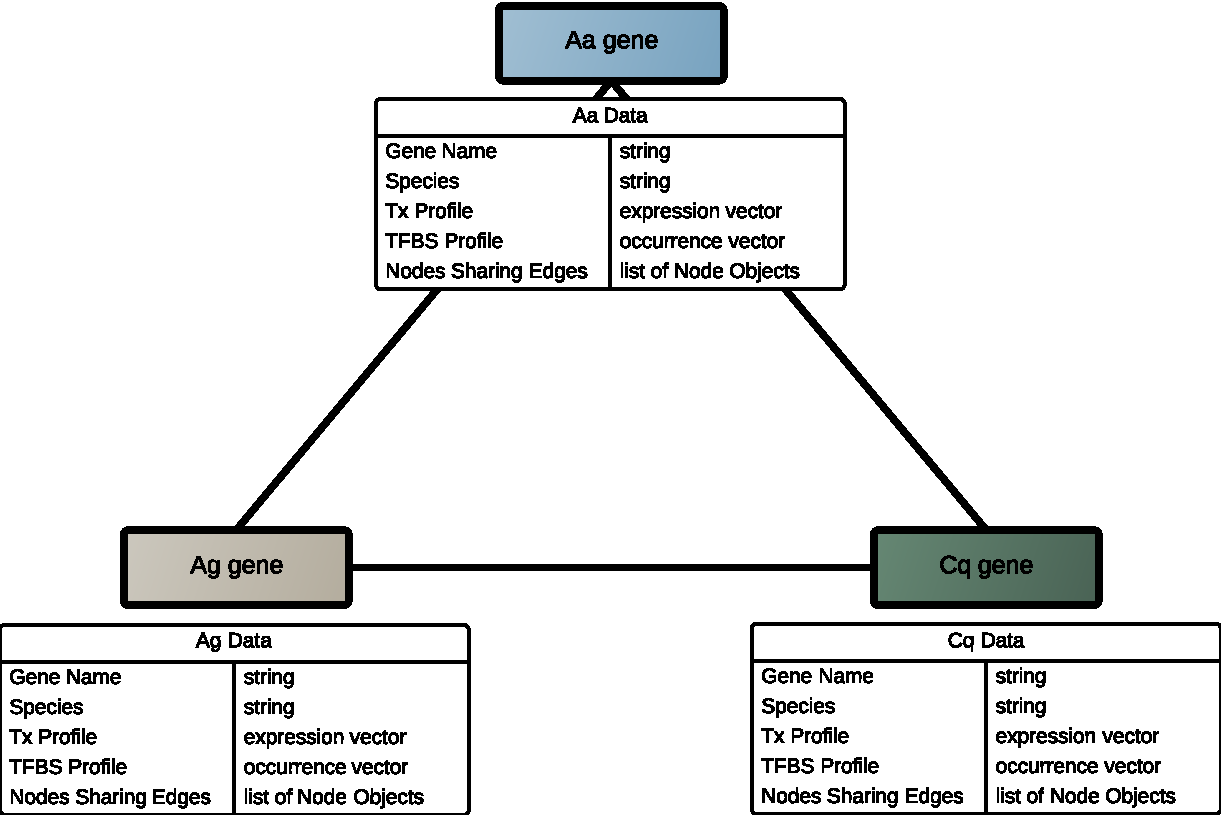
\includegraphics[width=\linewidth]{figures/figs/gfunc_graph_figs/ortho-graph-node-data.pdf}
    \caption{Node data model}\label{fig:nway-ortholog-graph-node-data}
    \end{subfigure}
% 
% 
% 
% 
% 
% 
    \begin{subfigure}[t]{.5\linewidth}
    \centering
    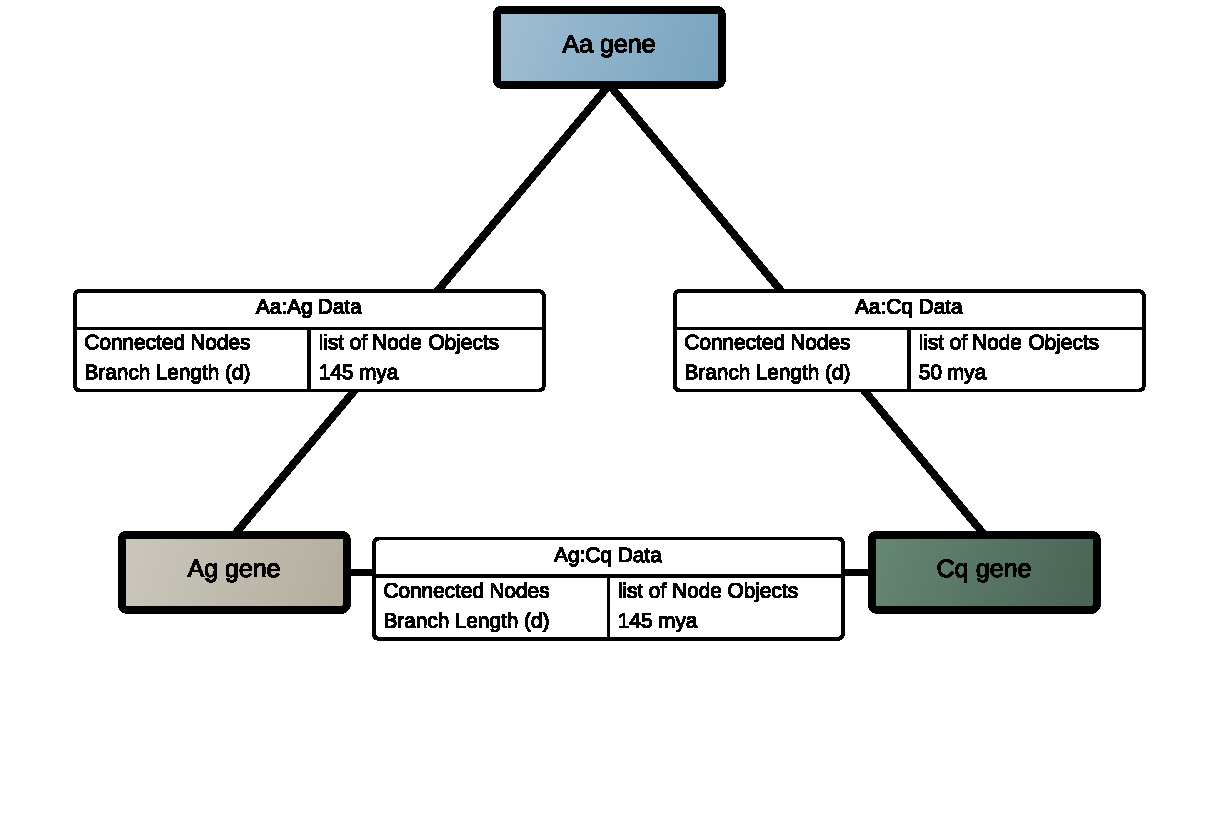
\includegraphics[width=\linewidth]{figures/figs/gfunc_graph_figs/ortho-graph-edge-data.pdf}
    \caption{Edge data model}\label{fig:nway-ortholog-graph-edge-data}
    \end{subfigure}%
% 
% 
%     
    \begin{subfigure}[t]{.5\linewidth}
    \centering
    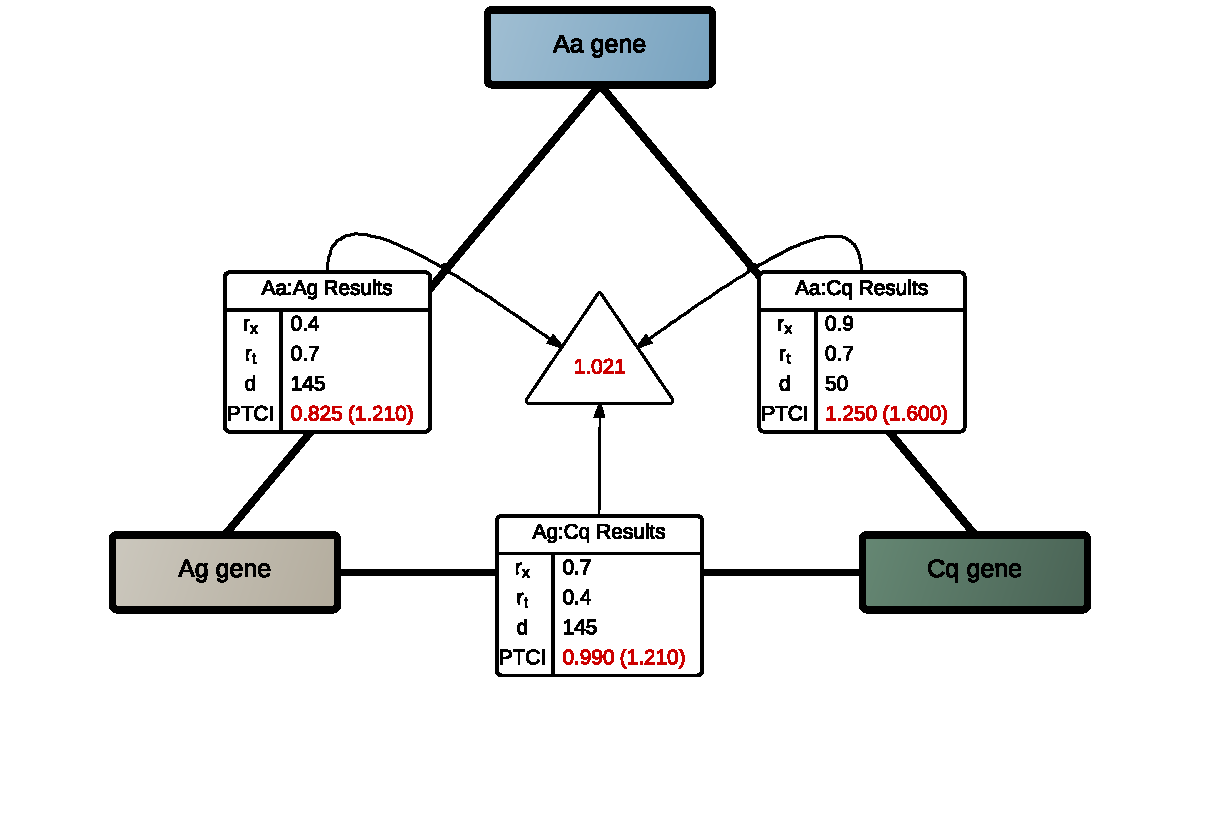
\includegraphics[width=\linewidth]{figures/figs/gfunc_graph_figs/ortho-graph-ptci.pdf}
    \caption{Example PTCI data}\label{fig:nway-ortholog-graph-ptci}
    \end{subfigure}
% 
% 
% 
\caption[Graph model used to integrate data types]{\sf \textbf{Graph model used to integrate data types.}}\label{fig:nway-ortholog-graph}
\end{figure}

The \gls{PTCI} fundamentally is a pairwise index.
The $N$-way 1:1 ortholog-sets in aggregate are scored by calculating the arithmetic mean of the respective pairwise 1:1 ortholog-sets (Figure \ref{fig:nway-ortholog-graph-ptci}).
Figure \ref{fig:nway-ortholog-graph-model} illustrates how a hypothetical 3-way 1:1 ortholog-set is related by 1:1 orthology between three species.
This is the fundamental graph-relationship representation that is modeled in the \gls{gFunc} code\footnote{See Section \ref{sec:custom-software}.}.






\section{Custom Software Solutions}\label{sec:custom-software}

Two core bodies of software were developed for this project as well as numerous smaller custom Python scripts.
\gls{blacktie} is a python package that automates data flow between and record keeping for analysis runs of the components of the third-party analysis pipeline dubbed the \gls{TuxProt} \cite{Trapnell2012}.
The purpose of the second software project, the \gls{gFunc}, is to provide a framework with which to integrate many, disparate data types to facilitate the synthesis of functional genomics analyses that make use of as many types of data as may be useful.

\gls{blacktie}'s code and documentation have been made available to the public.
It is hosted as a \gls{Git} project with the complete history of code commits included and available for easy open source improvement and collaboration.
It is also available as an easily installable package from the \gls{PyPI} for general users.
It has been downloaded and installed over 2000 times as of this time with its latest version (v0.2.1.2) being downloaded at least 327 times (according to \gls{PyPI}).

\gls{gFunc} is based around an existing, well known, and well maintained network-graph framework called networkx \cite{Hagberg2008}.
\gls{gFunc} uses this code library as a database backbone and provides a framework for installing common genomic data-types into the graph structure as well as a convention for extending the core objects of \gls{gFunc} to handle new types of data.
The project is not formally released.
After using it for my own work, I have learned more about how best to organize the code.
Once it has been re-factored to incorporate the lessons learned here (mainly that the core objects should be simplified as much as possible and more of the data management should be coded directly with networkx rather than re-implementing certain functions), it will be released to the public using the same mechanisms as described for \gls{blacktie}.


\subsection{Blacktie RNA-Seq pipeline}
Leveraging multiple fastQ files of \gls{RNA-Seq} reads into a coherent picture of gene expression and transcript models is a multi-step process.
Various analysis methods and corresponding programs exist and continue to be developed (DESeq \cite{Anders2010}, edgeR \cite{Robinson2010a}, eXpress \cite{Roberts2013}, MISO \cite{Katz2010}, Oases \cite{Schulz2012}, Trans-ABySS \cite{Robertson2010}).
The \gls{TuxProt} is a popular method with good documentation and user-support \cite{Trapnell2012}.
It consists of a coordinated data-flow through multiple complementary but stand-alone programs: \gls{tophat}, \gls{bowtie}, \gls{cufflinks}, \gls{cuffmerge}, \gls{cuffdiff}, and finally \gls{cummeRbund} \cite{Kim2013,Langmead2012,Trapnell2010,Goff2012}.
This requires the organization and coordination of many files of different types through many different program calls and output steps (Figure \ref{fig:tuxedo}).
Each step might take hours or days depending on the size of input data.
A further complication inherent to the use of swiftly evolving academic software is that new versions of the analysis software may be released after the analyses have been run but before the work has been published.
It is not uncommon for the latest version to give appreciably different results than the version originally used.



\begin{landscape}
 
 
 \begin{figure}[hp]
\centering
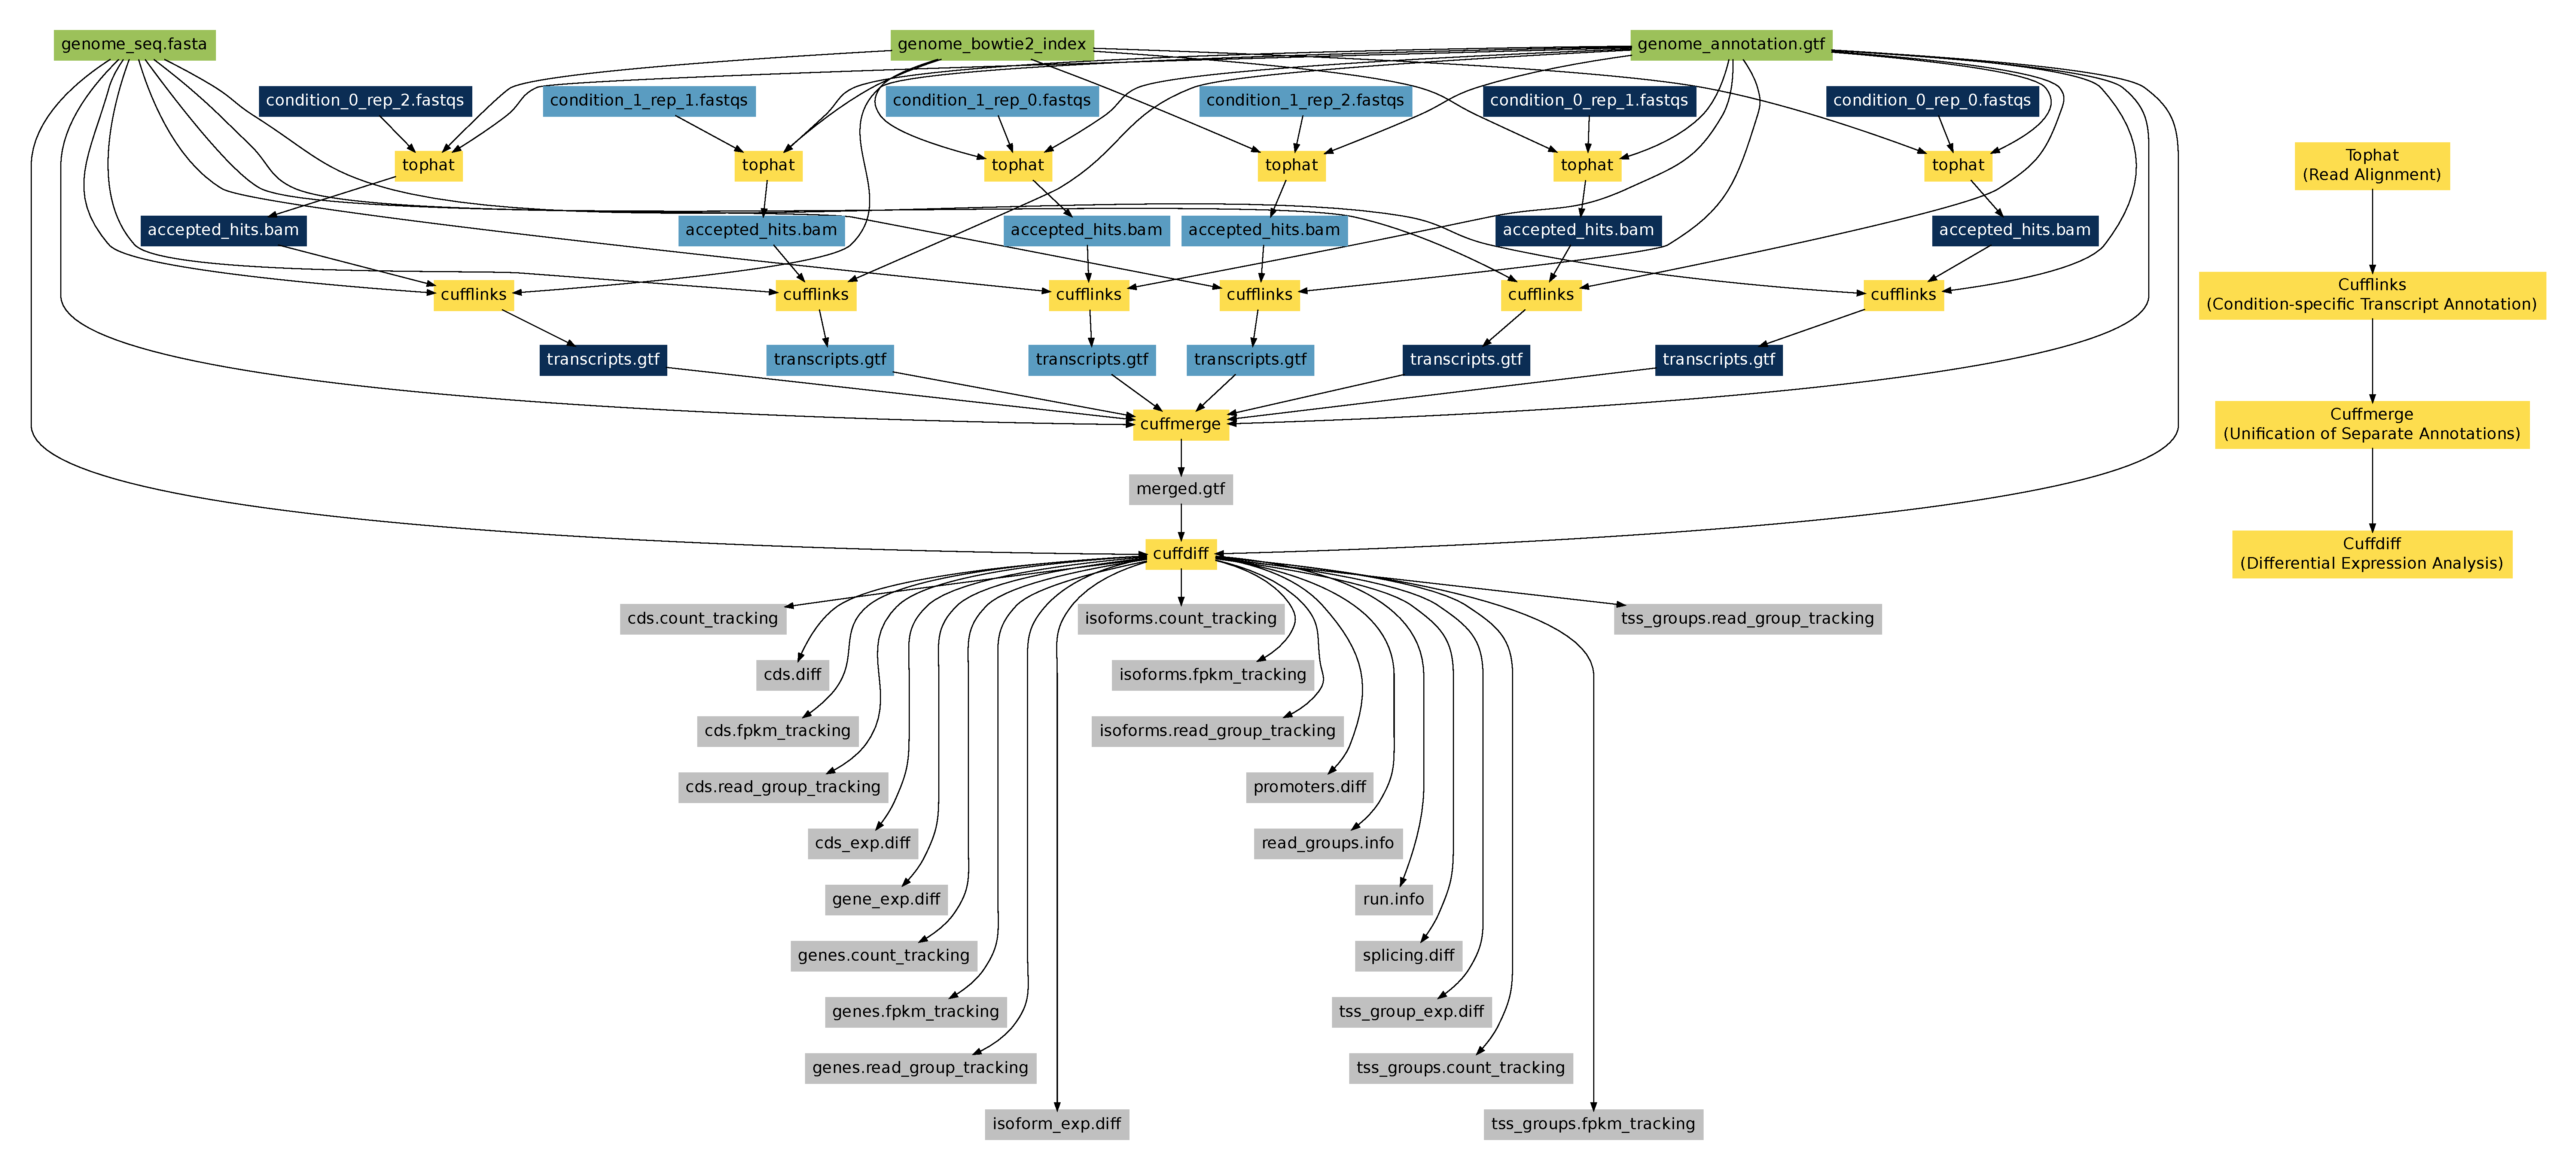
\includegraphics[width=\linewidth]{figures/figs/tuxedo_dot/707354_6/tophat_cufflinks_ins_outs.pdf}
\caption[Diagram of Abbreviated Tophat/Cufflinks Inputs and Outputs]{\sf \textbf{Diagram of Abbreviated Tophat/Cufflinks Inputs and Outputs:}\\
	This figure demonstrates the complexities of a typical RNA-seq experiment as analyzed with the \gls{TuxProt}. It models a fairly \textbf{simple} two condition experiment with each condition having three replications. It is ``abbreviated'' in that it only displays the output files that will be used in the next step for all steps except the \UseVerb{cuffdiff} step. The complete output of \UseVerb{cuffdiff} is included to demonstrate the final challenge of integrating the data which exists in multiple cross-referenced files.\\ 
	(\emph{Dark Blue} - Inputs/Outputs associated with Condition Zero; 
	\emph{Light Blue} - Inputs/Outputs associated with Condition One; 
	\emph{Grey} - Inputs/Outputs associated with Condition Zero \textbf{AND} Condition One; 
	\emph{Green} - Inputs Specific to the Reference Genome; 
	\emph{Gold} - Program Calls)
}
	\label{fig:tuxedo}
\end{figure}
 
 
 
\end{landscape}



The purpose of \gls{blacktie} is to streamline and simplify the complex task of analyzing full \gls{RNA-Seq} experiments using these programs; to record automatically settings used and program output messages so that users may track them later to data; provide a base-set of functions and classes that will allow users to create custom pipelines easily by editing a single file (or if they want: writing their own custom scripts).
For example, \gls{blacktie} makes the process of re-running an analysis from the point of an updated program more reliable because all settings and source-files are recorded automatically and made available alongside the original output.


Some other features include:

\begin{enumerate}
    \item simple installation
    \item simple command line interface that allows one to fully automate and reliably repeat their analysis of \gls{RNA-Seq} data using the \gls{TuxProt}
    \item ability to send email updates to the user
    \item intelligently continue with as much of the analysis as possible if a single branch of the pipeline fails
    \item analyze multiple, complex \gls{tophat}/\gls{cufflinks} experiments at once using a single command
    \item automatically generates \gls{SGE} scripts for use with a computing cluster
    \item checks the user's system for an R installation (required to run \gls{cummeRbund})
    \item checks for \gls{cummeRbund} library and walks user through installation if it is not currently installed
    \item automatic preliminary  \gls{cummeRbund} Quality Control, Basic Differential Expression, and Basic Pattern Discovery plots using cummeRbund
\end{enumerate}



\gls{blacktie} aims to bring automated, reproducible \gls{RNA-Seq} analysis with built-in record keeping to more researchers so that quality results may be obtained faster, easier and will contain fewer mistakes.



\subsection{gFunc framework for the integration and analysis of disparate genomic-scale data-types}

A common problem in the era of big data is how to incorporate many types of genome-scale data so that that the question at hand is meaningfully informed.
Relational databases such as MySQL or PostgreSQL have been used as data storage and analysis workhorses for decades at least.
Relational databases and graph-style databases each have performance advantages and disadvantages depending on the structure of the data and the most common operations expected to be carried out on the data.
However, a major advantage of graph-style models lies in the similarity that is shared with how many biologists conceptualize data and interactions between data entities.
A gene or protein can easily be conceptualized as a node with edges representing interactions or relationships\footnote{Edges may easily be conceptualized as many biologically relevant relationships such as homology, physical interactions, ancestor} between the nodes (Figure \ref{fig:ecrusp-graph}) \cite{Franceschini2013}.

\begin{figure}[h]
\centering
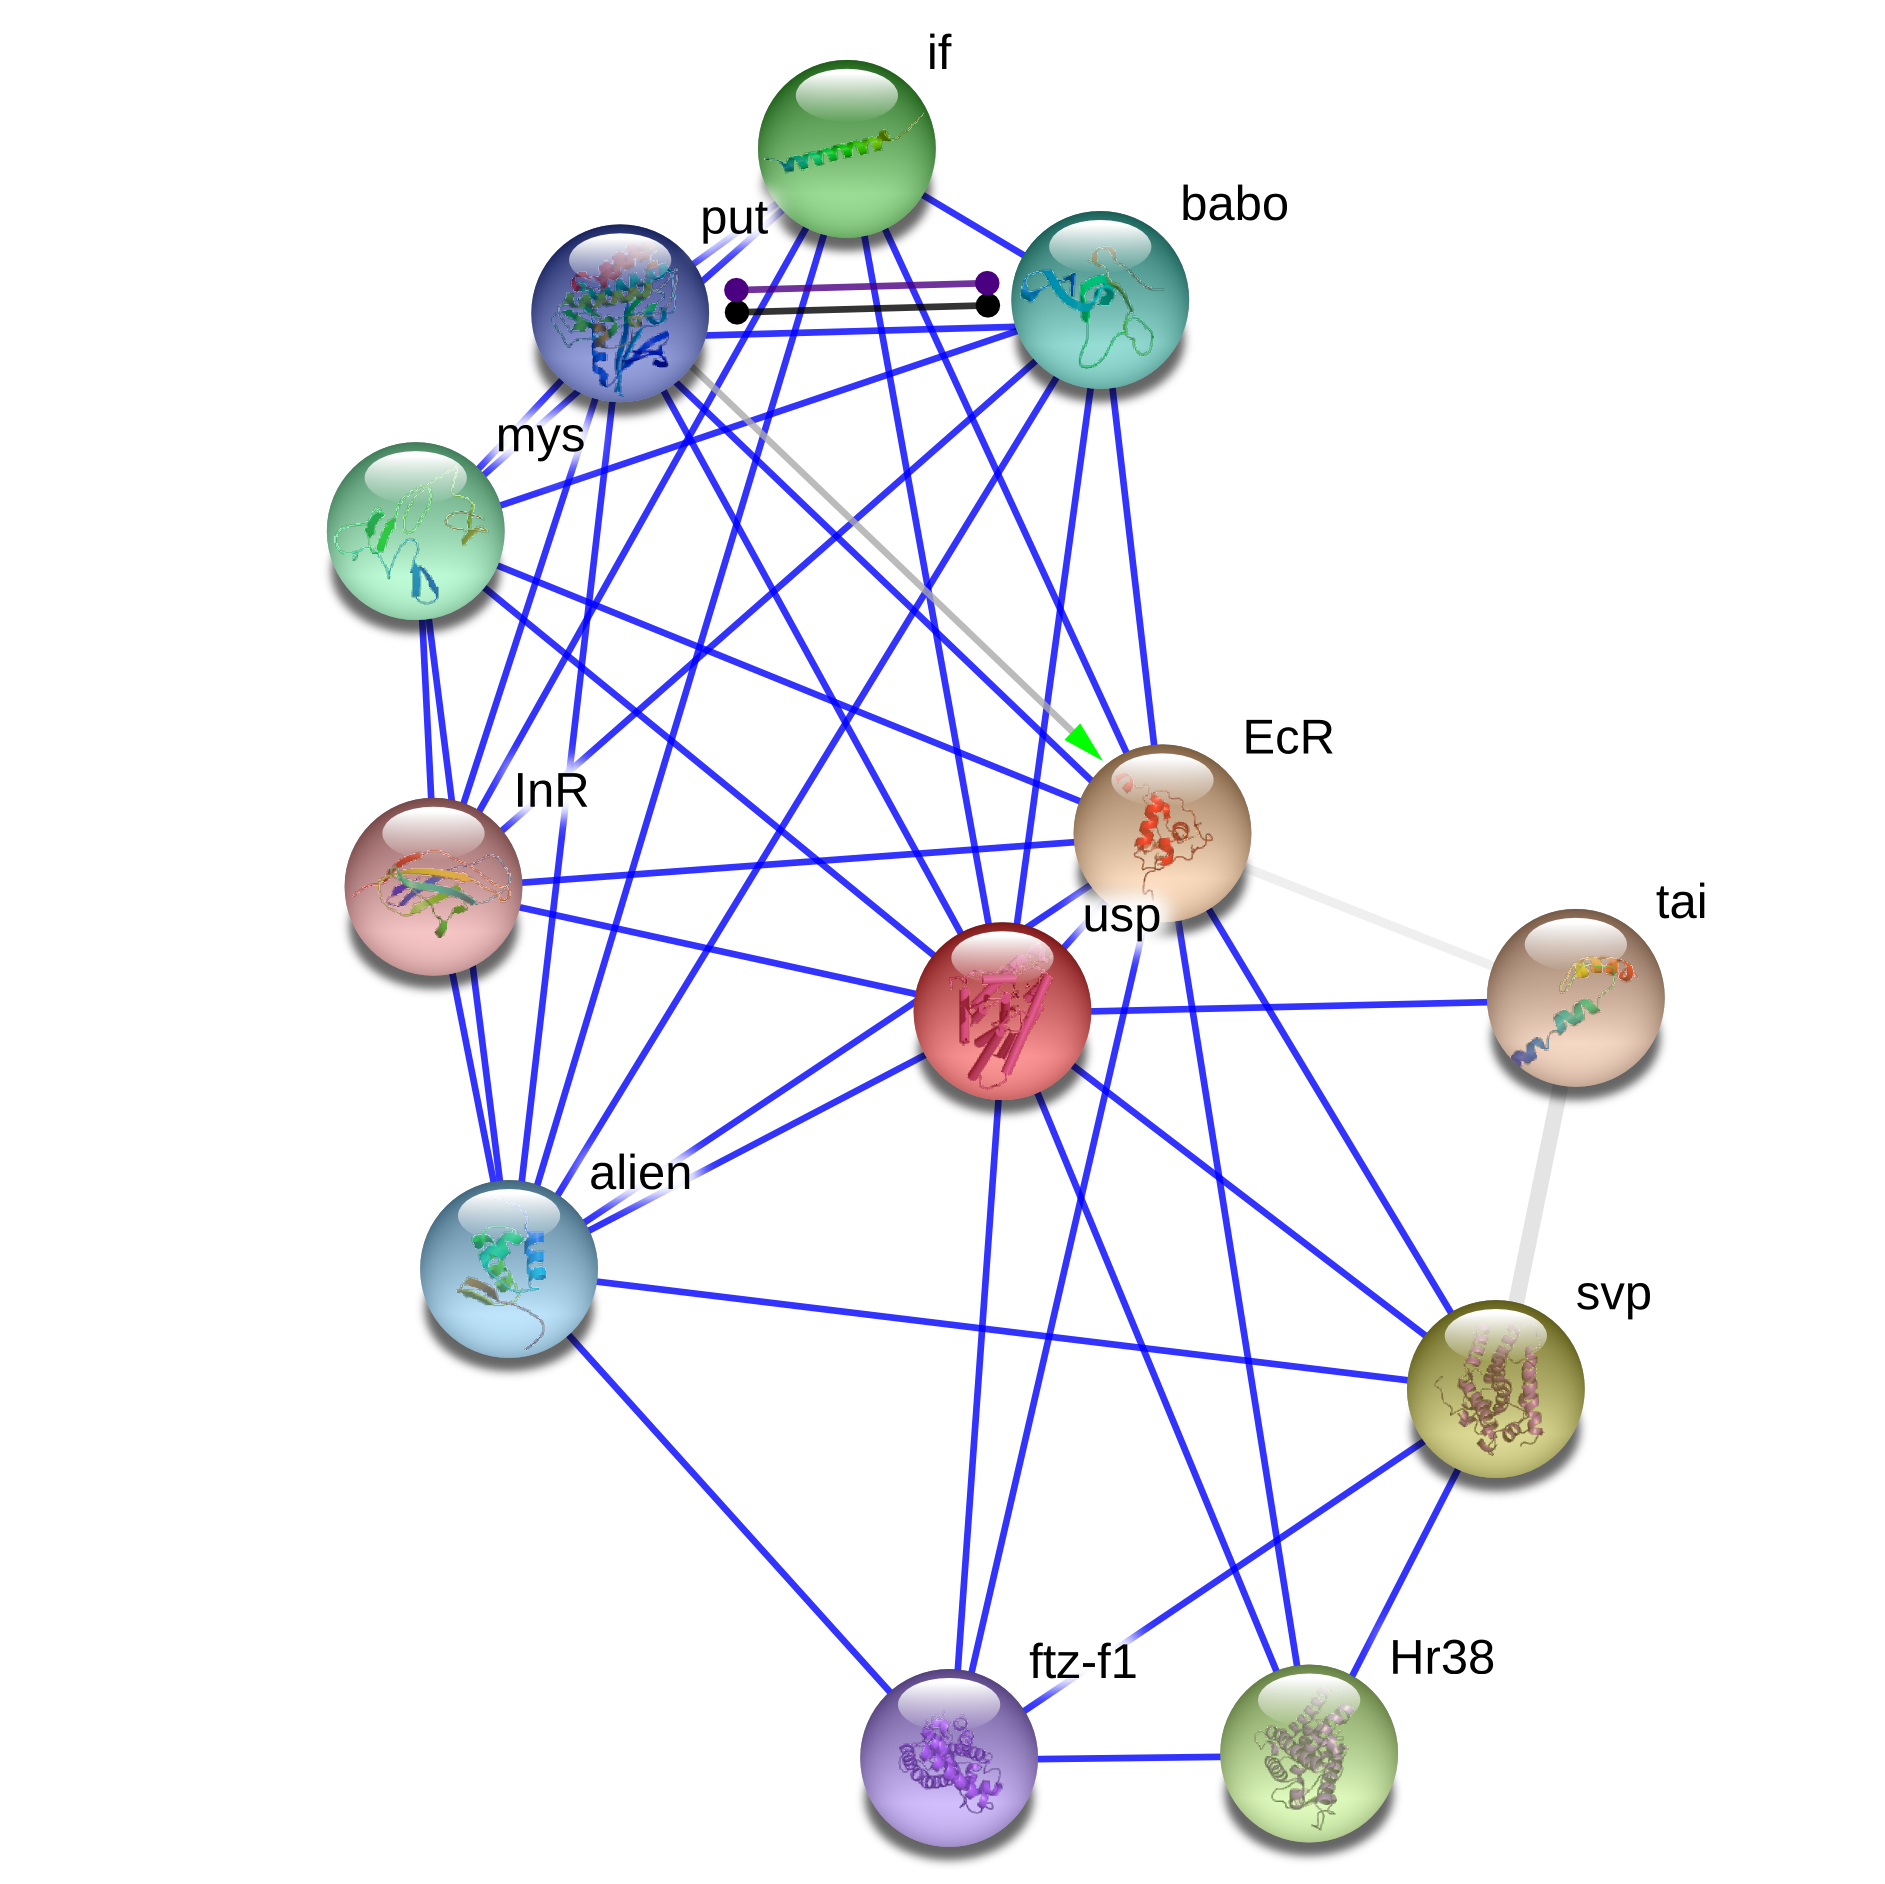
\includegraphics[width=.6\textwidth]{figures/figs/EcRUSP_graph.png}

\caption[Graphs are natural representations of biological relationships]{\sf \textbf{Graphs are natural representations of biological relationships.} Nodes (circles) represent proteins.
Edges (lines between nodes) represent interactions between nodes.
In a database scenario, edges and nodes can store multiple kinds of data in the form of key-value pair dictionaries (Figure \ref{fig:nway-ortholog-graph}) instead of a series of data tables grouped by a predefined schema as in relational databases.
}
\label{fig:ecrusp-graph}
\end{figure}


\subsubsection{Package Organization}
The code is organized around three fundamental types of classes.
The first type is made up of the data classes.
These model how data pertaining to nodes or edges are stored and accessed.
The second type of class consists of parser classes.
These consume a source file and convert the information into forms that can be loaded into data classes.
The third type are the graph tool classes (GraphBuilder, and GraphHandler).
These deal with mapping the parsed data onto the graph structure and help access the information from that graph as analyses are being performed, respectively.


The flexibility of this organization lies in the graph construction process.
The data parser classes encode specific information on how a single data-type is digested.
They all inherit a set of basic methods that control how data should be mapped to the graph, whether it is edge-data or node-data.
Because they all have this same graph-facing interface, the GraphBuilder does not need to know what kind of data the parser represents.
It simply is provided with a parser class, and it consumes that parser as the information streamed through the parser is correctly added to the graph.
Because of this format, it is straightforward to adapt the \gls{gFunc} system to accept new data-types.
One simply needs to write a parser class that inherits from the base parser class and include the correct rules for parsing the new data-type.
That new parser can be included in a list of existing parser classes to be provided to the GraphBuilder and the new data will be correctly added into the graph structure.

The GraphHandler stores the graph and provides conveniences for accessing its contents, such as node and edge dictionaries.


\section{gFunc-based analysis}
Once the preliminary data preparation is accomplished (Section \label{sec:prelim-data}), the data is loaded into a \gls{gFunc} graph through a script (\texttt{gfunc\_build\_n\_way\_one2one.py} \cite{Dunn2013dissSupl}) that coordinates the initiation of relevant parsers and provides them to a GraphBuilder object that maps the data onto the 3-way 1:1 ortholog-relationships.
\glspl{FDR} are empirically estimated by calculating all 3-way-\gls{PTCI} values first using the real 3-way 1:1 ortholog relationships, then repeating the analysis many times with randomized (null) 3-way 1:1 orthology relationships.
\alert{(for what follows: should i refer to the figure from the next chapter here?  Its kinda like having results in the methods section?)}
The \gls{FDR} is then defined, for a given 3-way-\gls{PTCI} threshold, as the median value of the null 3-way \glspl{PTCI} divided by the actual 3-way \gls{PTCI} (\texttt{PTCI\_testing\_rsrd\_1.0\_1.1\_new\_data\_Jaspar\_nr\_insect\_20130918\_orthodb7.ipynb} \cite{Dunn2013dissSupl}).
This information is used to define an acceptable 3-way-\gls{PTCI} threshold that balances selectivity with sensitivity.
Given a 3-way-\gls{PTCI} threshold, a filter script (\texttt{Getting\_and\_using\_filtered\_gfunc\_genes\_ecr\_team\_OR\_jaspar\_insect\_20120918\_orthodb7.ipynb} \cite{Dunn2013dissSupl}) is applied to extract the 3-way 1:1 ortholog sets that are greater than or equal to the threshold.

This process is carried out using two sets of \gls{TFBS} profile data: one that covers the entire JASPAR \gls{TFBS}-model database for insects (\texttt{JASPAR\_CORE\_2009\_insects.meme}  \cite{Dunn2013dissSupl}), another that is limited to 12 \gls{TFBS}-models that are thought to participate in \gls{20E}-regulated transcriptional regulatory mechanisms (\texttt{EcR\_team.meme} \cite{Dunn2013dissSupl}).
The later is meant to provide a set of 3-way 1:1 orthologs generated with a focus toward a particular regulatory program while the former is intended to capture a more general set.
The union of the two result-sets are taken forward to the Characterization Stage.



\section{Characterization of results} \label{chap:3-sec:characterization-of-results}
The \gls{gFunc} analysis yields a set of the top midgut transcriptionally corresponding 3-way 1:1 ortholog-sets.
Two types of characterization were carried out on these ortholog-sets.
The characterization method used \gls{Argot2} to obtain functional annotations of the ortholog-sets by comparing the protein sequences of the 3-way 1:1 ortholog-sets against previuosly annotated proteins (\gls{Swiss-Prot}) and hidden markov-models of described protein domains (\gls{Pfam}) \cite{Boeckmann},\cite{Punta2012},\cite{Falda2012}.
The second method consisted of grouping the \glspl{mAP} by similarity using k-means clustering.

\subsection{Functional inference of filtered 3-way 1:1 ortholog sets}

\gls{Argot2} was used to infer functional annotations for the selected proteins of the three mosquito species.
First, the peptide sequences must be compared with well characterized databases of functinally annotated data.
\gls{Argot2} suppports the use of either the Swiss-Prot\footnote{Swiss-Prot is the manually annotated and reviewed section of the UniProt Knowledgebase.} database of protein sequences or the \gls{Pfam}\footnote{The Pfam database is a large collection of protein families, each represented by multiple sequence alignments and \glspl{HMM}.} database of protein domain models or both.
Here both were used.

The following blastp settings were used against the \gls{Swiss-Prot} proteins, as requested by the \gls{Argot2} instructions:

\begin{Verbatim}
blastp -outfmt "6 qseqid sseqid evalue " -query your_sequences \
      -db Uniprot -out output_file
\end{Verbatim}

Likewise, the following HMMER3 settings were used against the \gls{Pfam} domain models\footnote{The Pfam-A (hand-currated models) and Pfam-B (automated curration) databases were combined as suggested by \gls{Argot2}.}, as requested by the \gls{Argot2} instructions:


\begin{Verbatim}
hmmscan --tblout output_file P-fam_database your_protein_sequences
\end{Verbatim}

Both sets of results were then compressed into ``zip'' files and uploaded to the \gls{Argot2} servers for analysis.

\subsection{Clustering of filtered 3-way 1:1 ortholog sets} \label{chap:3-sec:clustering-of-filtered-ortholog-sets}

Clusters were generated by custom python code that used Biopython's k-means clustering (version 1.62) \cite{Cock2009}.
\gls{mAP} data was log transformed after 1 FPKM was added to all data to remove zeros ($log_{10}(\mathrm{FPKM}+1)$). 
K-means was then applied using the arithmetic mean as the center for cluster definition.
Twenty-three clusters ($k = 23$) were used.
The clustering was performed using the \glspl{mAP} from \Ag\ because this species is approximately equidistant from the other two with regard to a last common ancestor.
Four of the resulting clusters were chosen for further description in Chapter \ref{chap:4} and the orthologs of the corresponding members of each cluster from \Aa\ and \Cq\ were retrieved and combined with those from \Ag.
The four clusters were chosen because they exhibit a major change between \gls{NBF} and 4h \gls{PBM}\footnote{There is a small but reproducible peak in \gls{20E} titers that occurs 4h \gls{PBM} \cite{Hagedorn1975} and coincides with a peak in posterior midgut aminopeptidase activity that has been noted in \As\ \cite{Billingsley1991}; an initiation of the increase of late trypsin in the midgut \cite{Barillasmury1991},\cite{Graf1988}; and an increase of JH-esterase activity that causes a rapid decline of \gls{JH} \cite{Shapiro1986}.} samples that may indicate the \glspl{mAP} contained in these clusters are influenced by \gls{20E}-regulated transcriptional regulatory mechanisms.
The four patterns can be described roughly as ``up-regulated \textit{at} 4h \gls{PBM}'', ``down-regulated \textit{at} 4h \gls{PBM}'', ``up-regulated \textit{after} 4h \gls{PBM}'', and ``down-regulated \textit{after} 4h \gls{PBM}''.




%%% Local Variables: ***
%%% mode: latex ***
%%% TeX-master: "thesis.tex" ***
%%% End: ***

\chapter{Results and Discussion} \label{chap:4}

% \section{Preliminary data preparation stage}
% 
% These results pertain to the first stage of the approach described in Chapter \ref{chap:3} (Figure \ref{fig:approach-chart}: \textit{salmon box}).

\section{gFunc-based analysis stage}

These results pertain to the second stage of the approach described in Chapter \ref{chap:3} (Figure \ref{fig:approach-chart}: \textit{yellow box}).

\paragraph*{Complementary sets of TFBS models:}
\gls{PTCI} data was calculated using two complementary sets of \gls{TFBS} models.
%
One set focuses the \gls{PTCI} on genes that have been associated with \gls{20E} and its nuclear receptor (\PTCIe) (Figures \ref{fig:ecr-pair-ptci-hists} and \ref{fig:ecr-mean-ptci-hists}), and a second provides a general focus on \gls{TFBS} models provided by JASPAR that are defined in insects at large (\PTCIi) (Figures \ref{fig:insect-pair-ptci-hists} and \ref{fig:insect-mean-ptci-hists}).
%

\begin{figure}[hp]
%
\subcaptionbox{\label{fig:ecr-pair-ptci-hists-base}}
{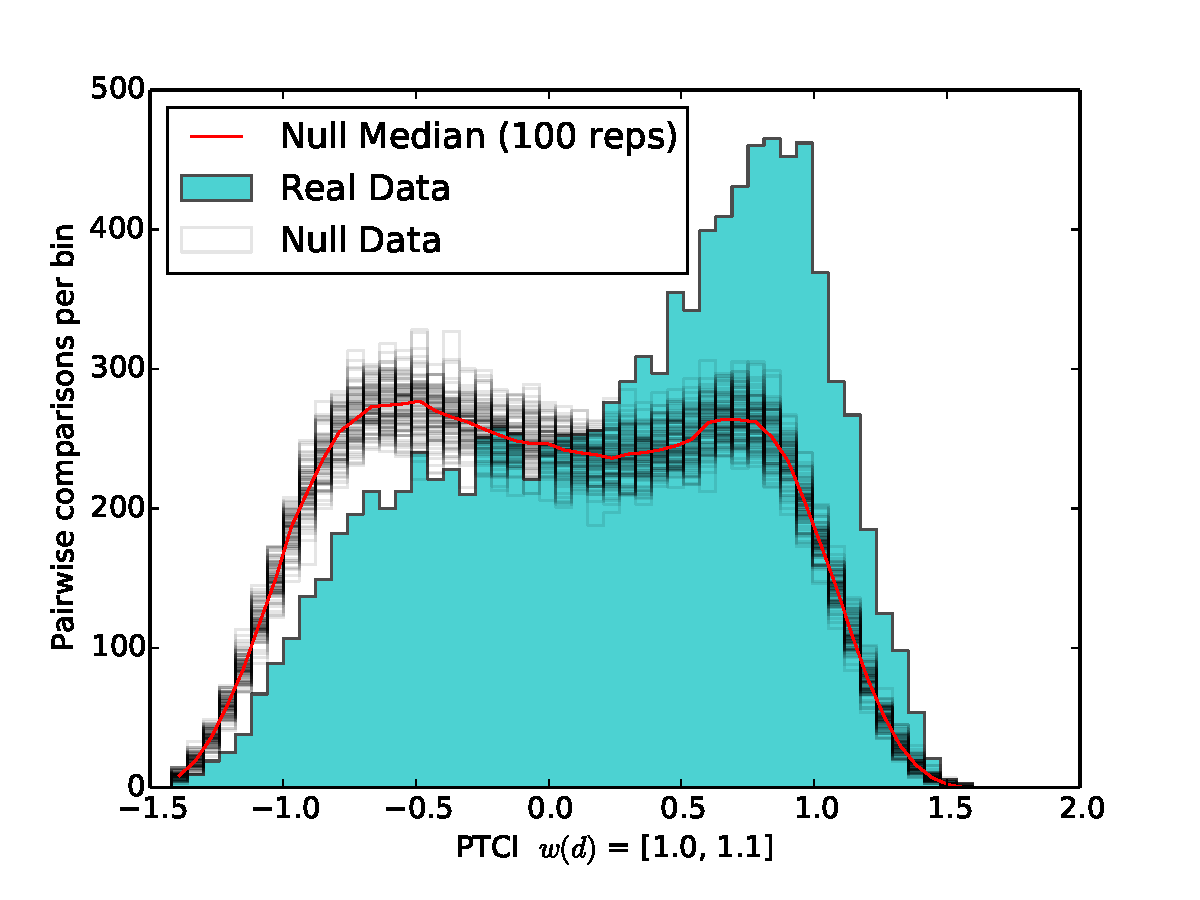
\includegraphics[width=.5\linewidth]{figures/figs/ecr_team_ptci_20130918_orthodb7/pairwise_ptci_hist.pdf}}
% 
\subcaptionbox{\label{fig:ecr-pair-ptci-hists-rcum-hist}}
{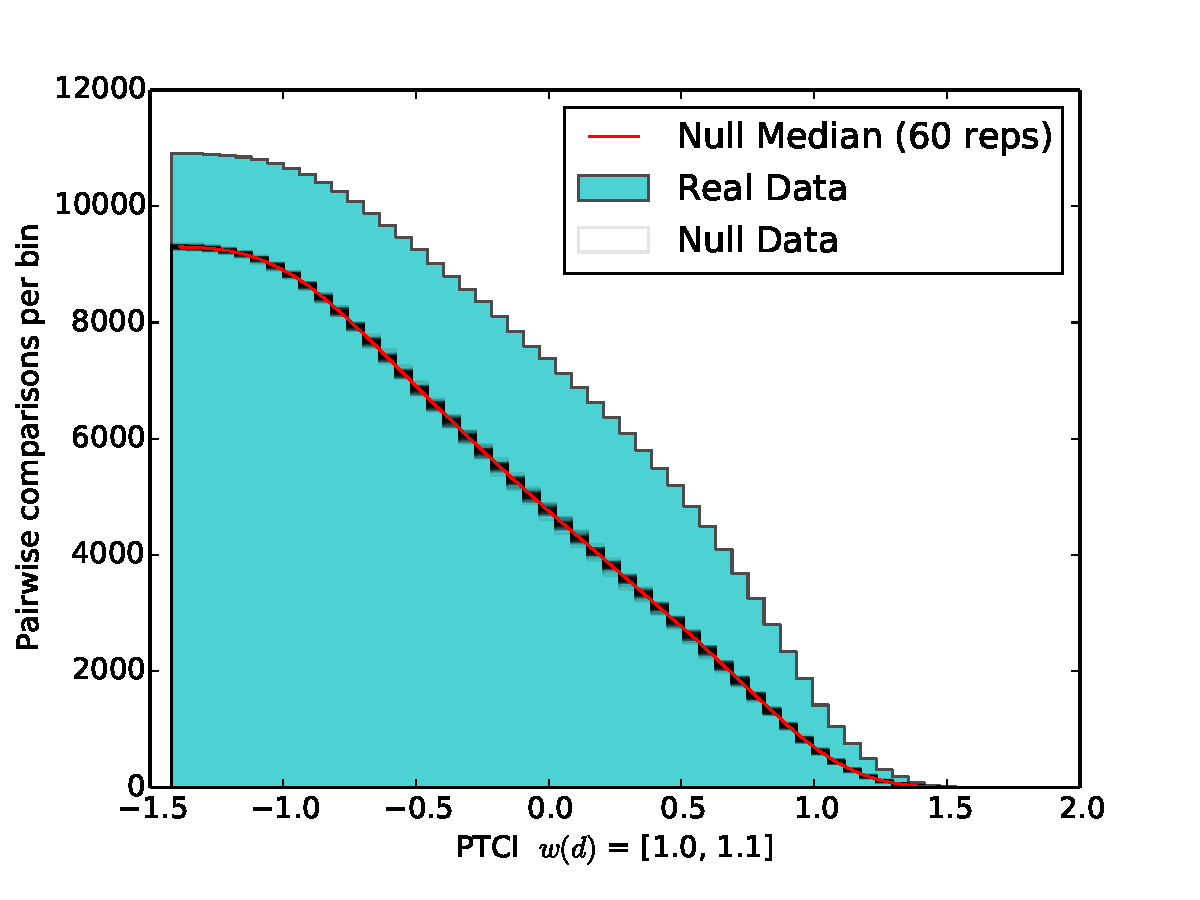
\includegraphics[width=.5\linewidth]{figures/figs/ecr_team_ptci_20130918_orthodb7/pairwise_ptci_cum_hist.pdf}}
% 
\subcaptionbox{\label{fig:ecr-pair-ptci-hists-fdr}}
{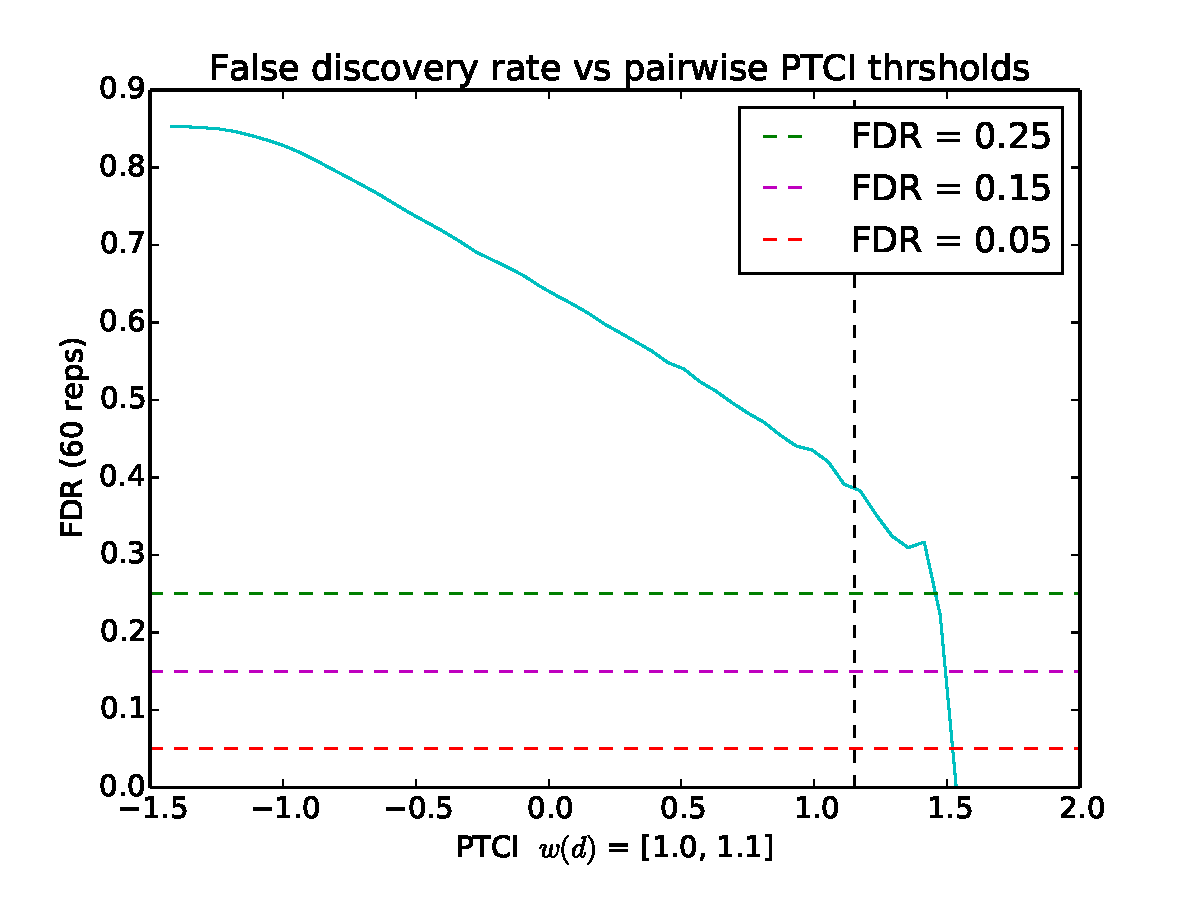
\includegraphics[width=.5\linewidth]{figures/figs/ecr_team_ptci_20130918_orthodb7/pairwise_ptci_fdr.pdf}}
% 
% 
\caption[Pairwise 20E-PTCI results]{\sf \textbf{Pairwise PTCI results for the \gls{20E}-\gls{TFBS} group}:\\
\textbf{(A)} Histogram of mean PTCI results vs null distributions.
\textbf{(B)} Reverse Cumulative histogram of mean PTCI results vs null distributions.
\textbf{(C)} False discover rate vs PTCI threshold.}
\label{fig:ecr-pair-ptci-hists}
\end{figure}

\begin{figure}[hp]
%
\subcaptionbox{\label{fig:ecr-mean-ptci-hists-base}}
{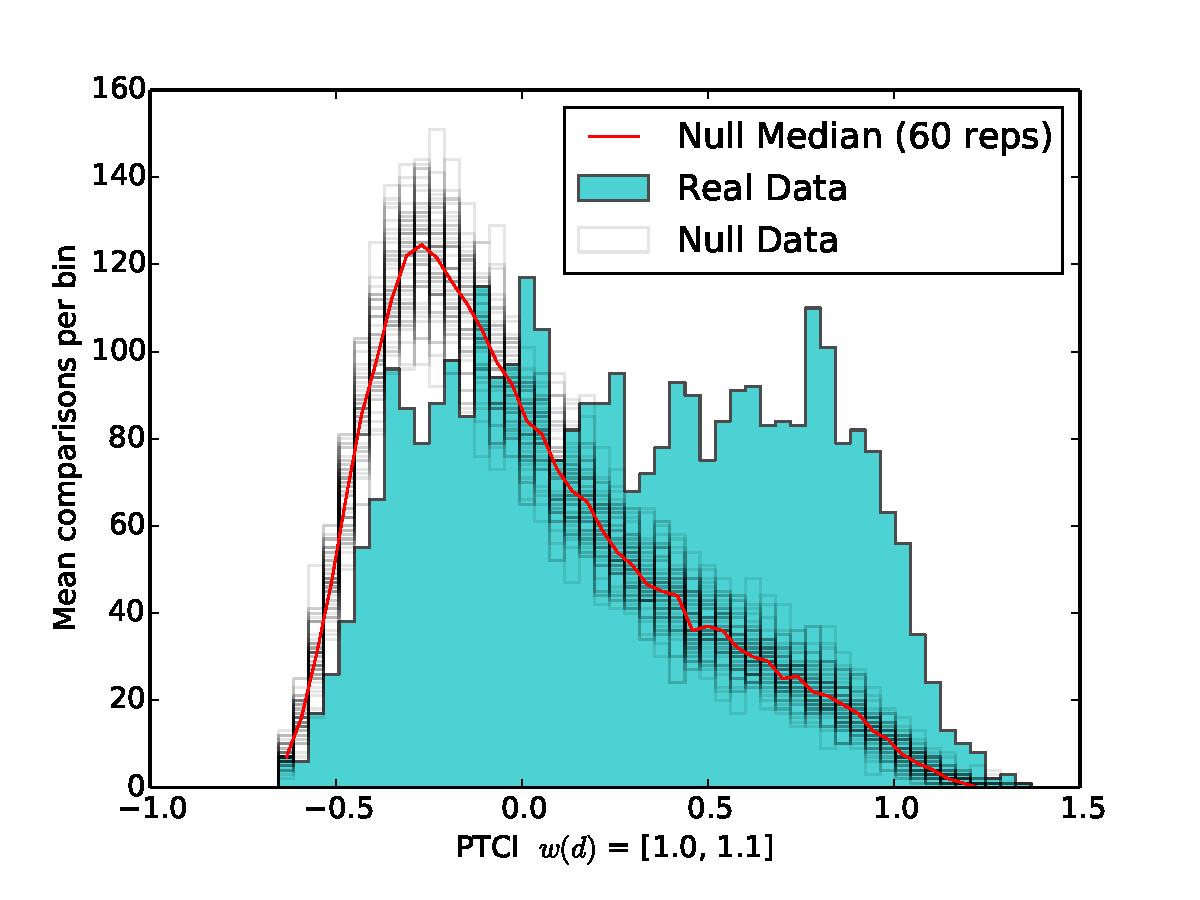
\includegraphics[width=.5\linewidth]{figures/figs/ecr_team_ptci_20130918_orthodb7/mean_ptci_hist.pdf}}
% 
\subcaptionbox{\label{fig:ecr-mean-ptci-hists-rcum-hist}}
{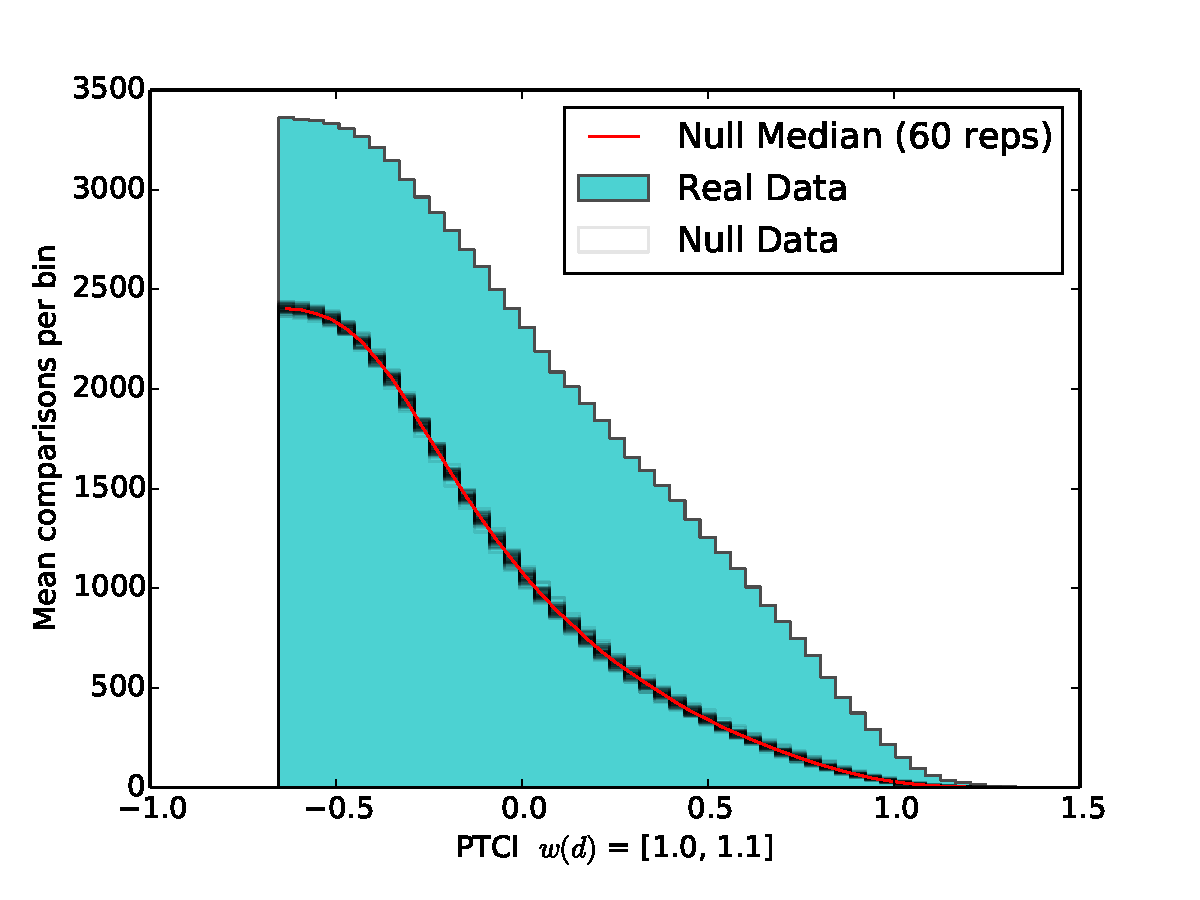
\includegraphics[width=.5\linewidth]{figures/figs/ecr_team_ptci_20130918_orthodb7/mean_ptci_cum_hist.pdf}}
% 
\subcaptionbox{\label{fig:ecr-mean-ptci-hists-fdr}}
{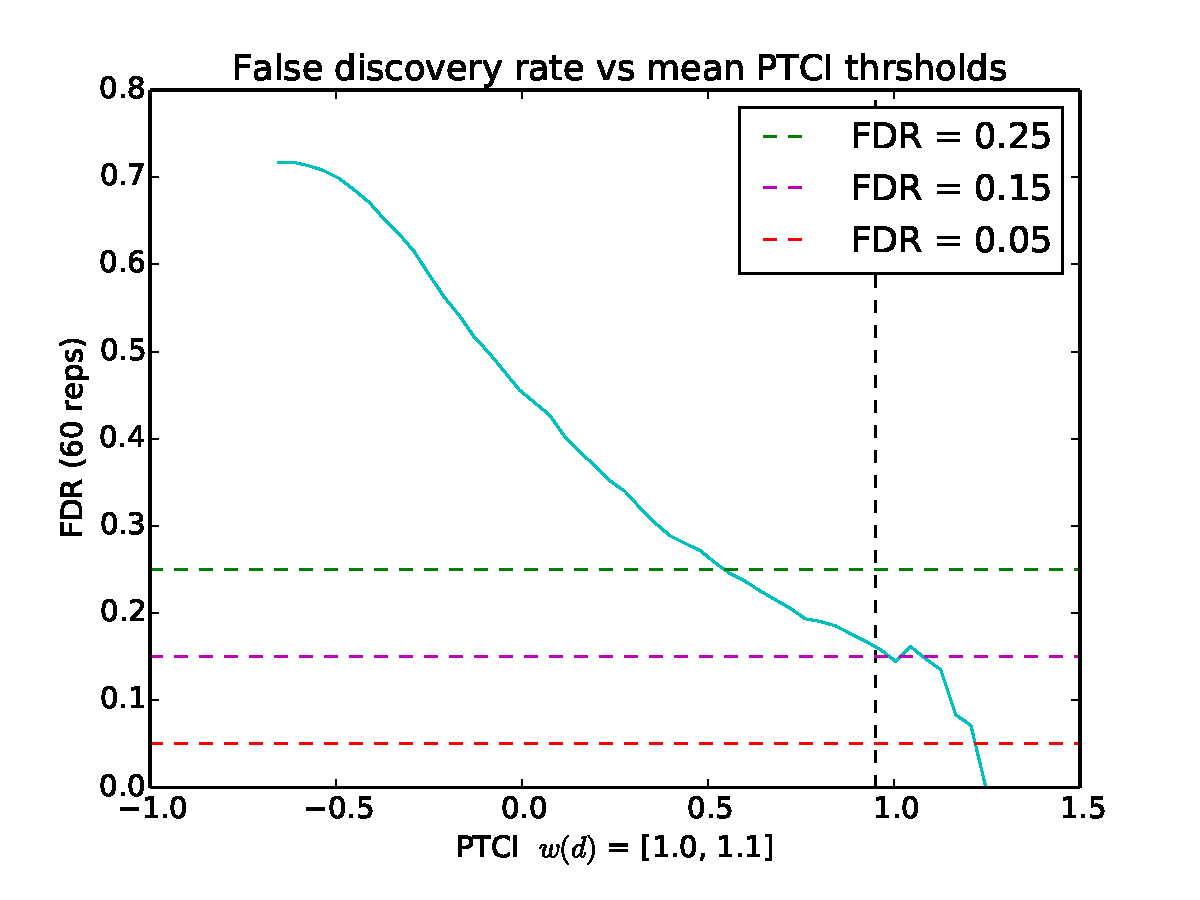
\includegraphics[width=.5\linewidth]{figures/figs/ecr_team_ptci_20130918_orthodb7/mean_ptci_fdr.pdf}}
% 
% 
\caption[Mean 20E-PTCI results]{\sf \textbf{Mean PTCI results for the \gls{20E}-\gls{TFBS} group}:\\
\textbf{(A)} Histogram of mean PTCI results vs null distributions.
\textbf{(B)} Reverse Cumulative histogram of mean PTCI results vs null distributions.
\textbf{(C)} False discovery rate vs PTCI threshold.}
\label{fig:ecr-mean-ptci-hists}
\end{figure}

\begin{figure}[hp]
%
\subcaptionbox{\label{fig:insect-pair-ptci-hists-base}}
{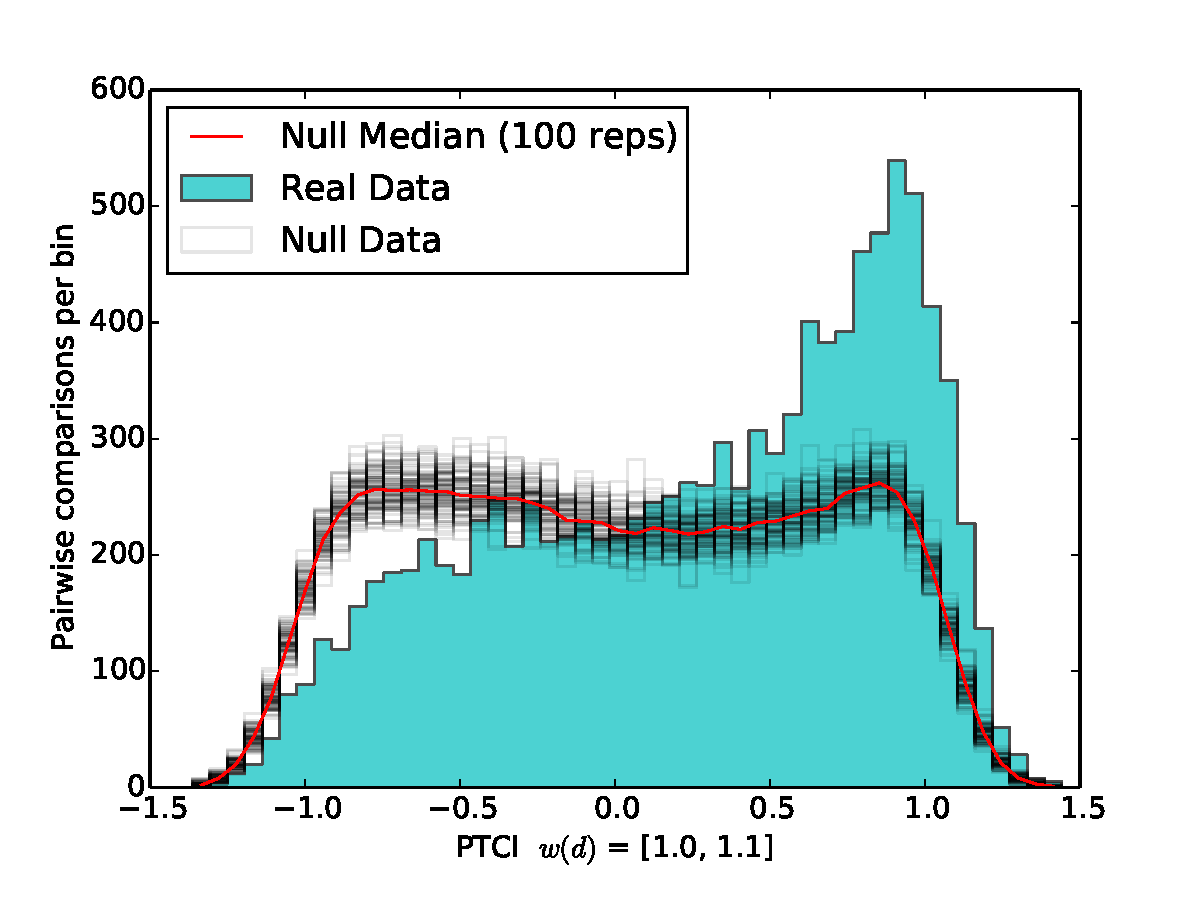
\includegraphics[width=.5\linewidth]{figures/figs/jaspar_insect_ptci_20130918_orthodb7/pairwise_ptci_hist.pdf}}
% 
\subcaptionbox{\label{fig:insect-pair-ptci-hists-rcum-hist}}
{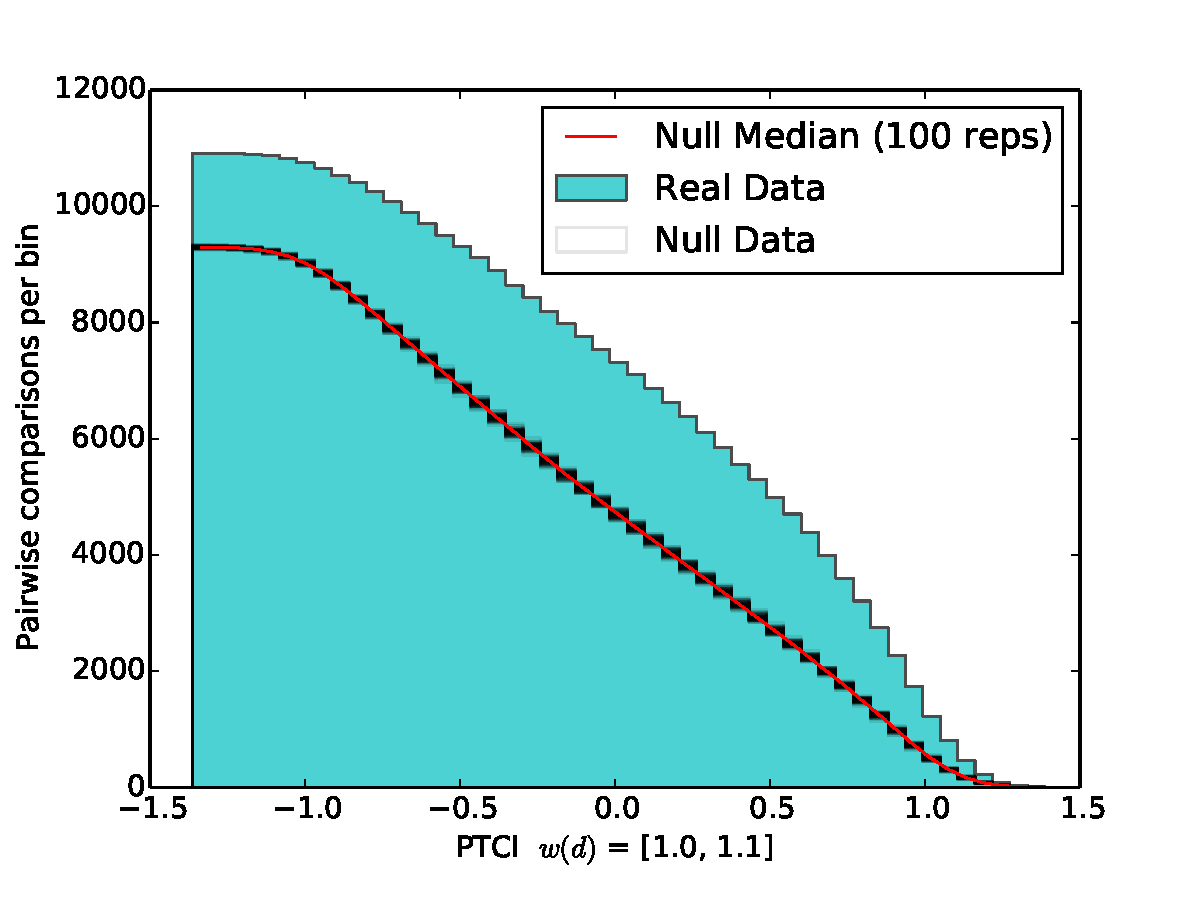
\includegraphics[width=.5\linewidth]{figures/figs/jaspar_insect_ptci_20130918_orthodb7/pairwise_ptci_cum_hist.pdf}}
% 
\subcaptionbox{\label{fig:insect-pair-ptci-hists-fdr}}
{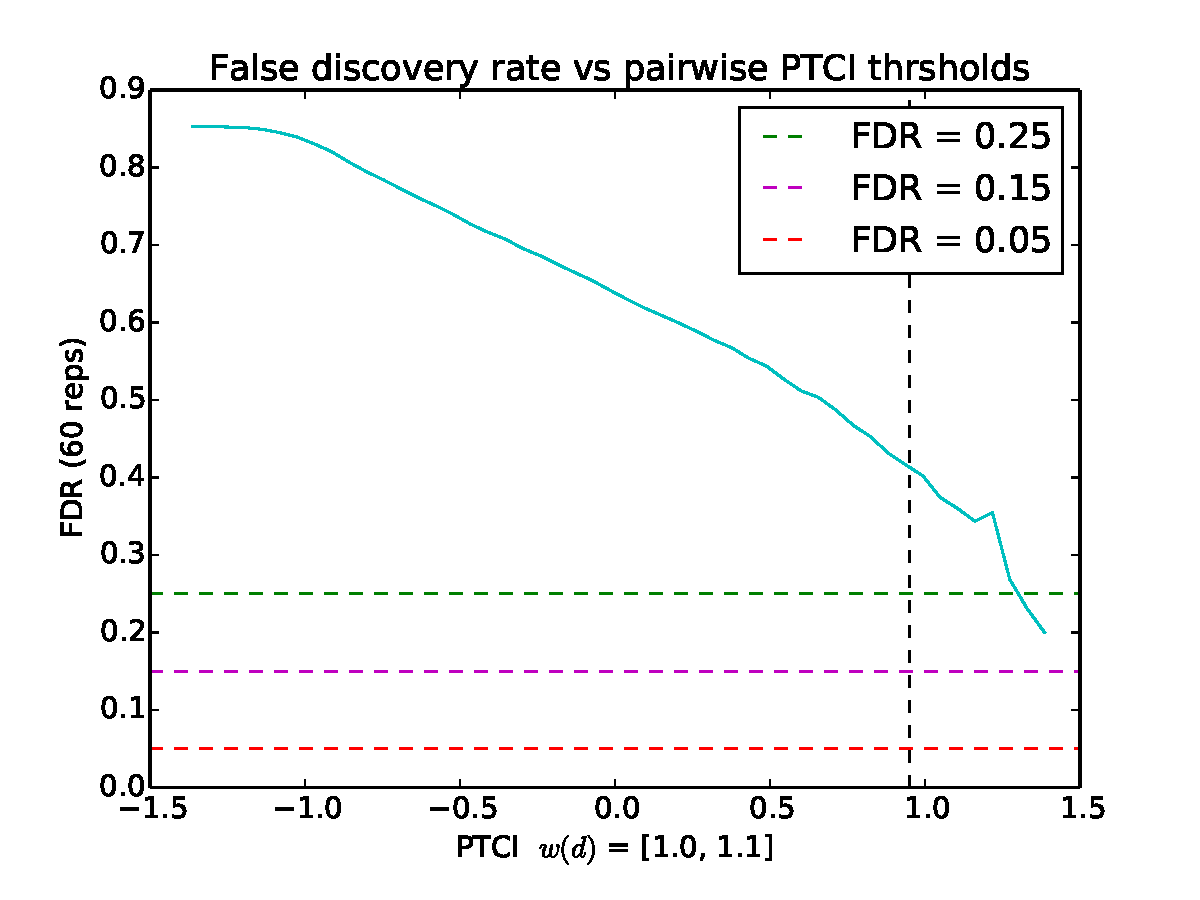
\includegraphics[width=.5\linewidth]{figures/figs/jaspar_insect_ptci_20130918_orthodb7/pairwise_ptci_fdr.pdf}}
% 
% 
\caption[Pairwise insect-PTCI results]{\sf \textbf{Pairwise PTCI results for the insect-\gls{TFBS} group}:\\
\textbf{(A)} Histogram of mean PTCI results vs null distributions.
\textbf{(B)} Reverse Cumulative histogram of mean PTCI results vs null distributions.
\textbf{(C)} False discover rate vs PTCI threshold.}
\label{fig:insect-pair-ptci-hists}
\end{figure}

\begin{figure}[hp]
% /home/gus/Dropbox/repos/git/uci-thesis-latex/figures/figs/jaspar_insect_ptci_20130918_orthodb7/mean_ptci_cum_hist.pdf
\subcaptionbox{\label{fig:insect-mean-ptci-hists-base}}
{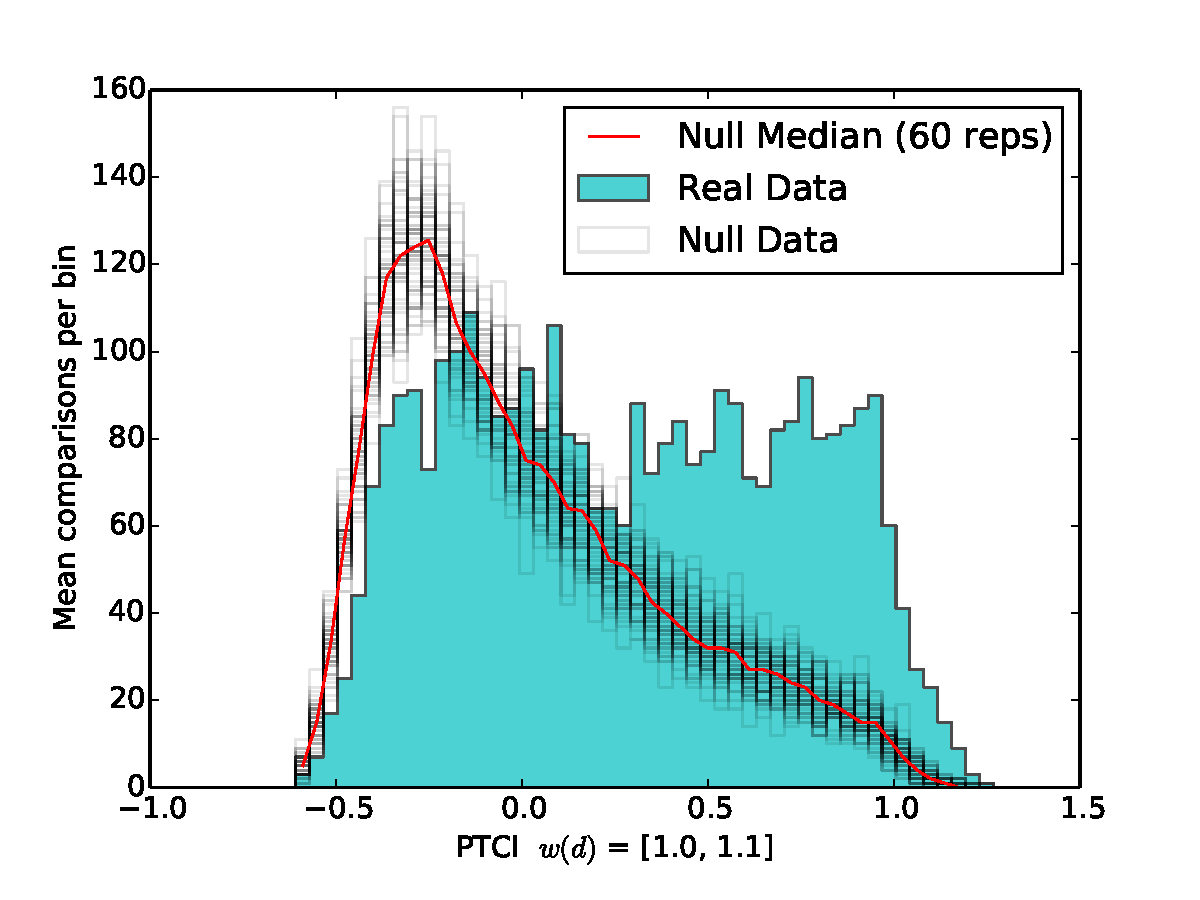
\includegraphics[width=.5\linewidth]{figures/figs/jaspar_insect_ptci_20130918_orthodb7/mean_ptci_hist.pdf}}
% 
\subcaptionbox{\label{fig:insect-mean-ptci-hists-rcum-hist}}
{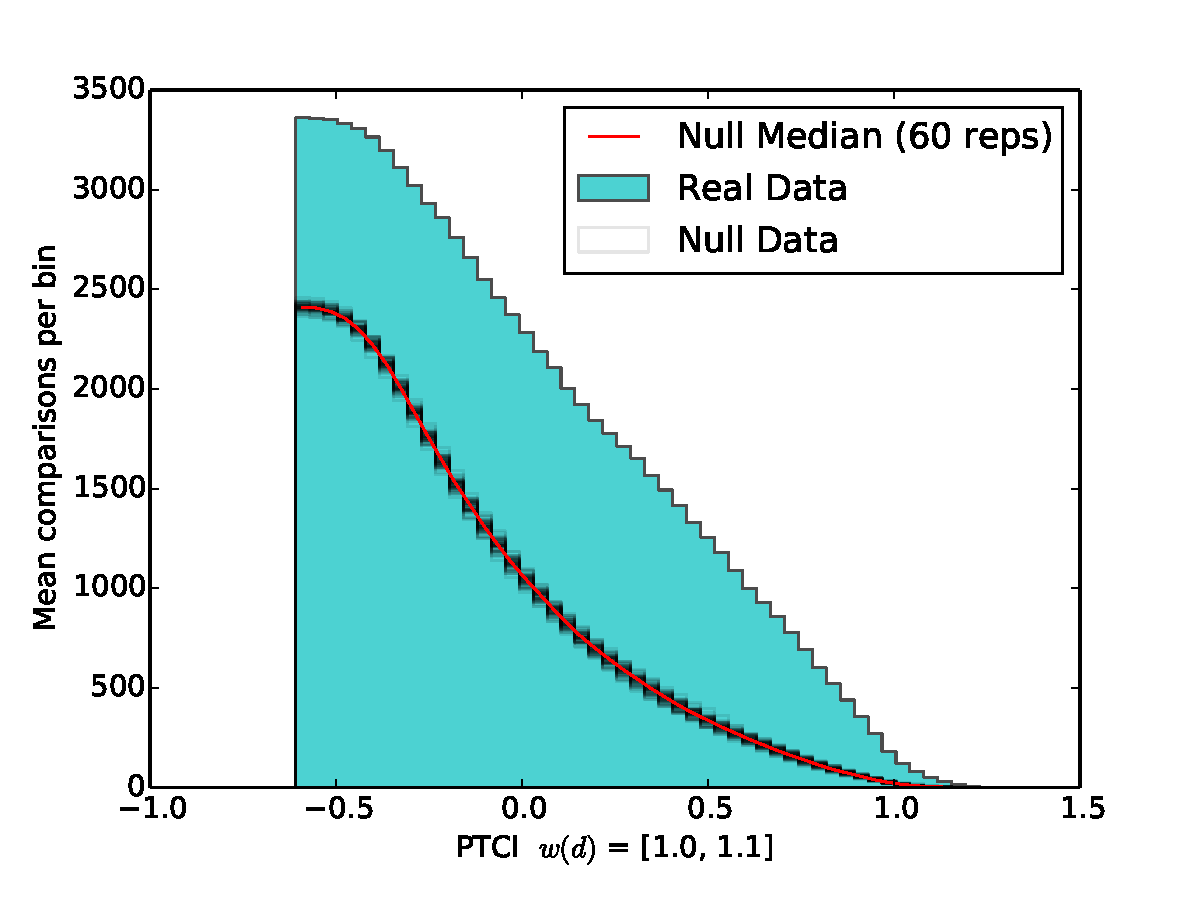
\includegraphics[width=.5\linewidth]{figures/figs/jaspar_insect_ptci_20130918_orthodb7/mean_ptci_cum_hist.pdf}}
% 
\subcaptionbox{\label{fig:insect-mean-ptci-hists-fdr}}
{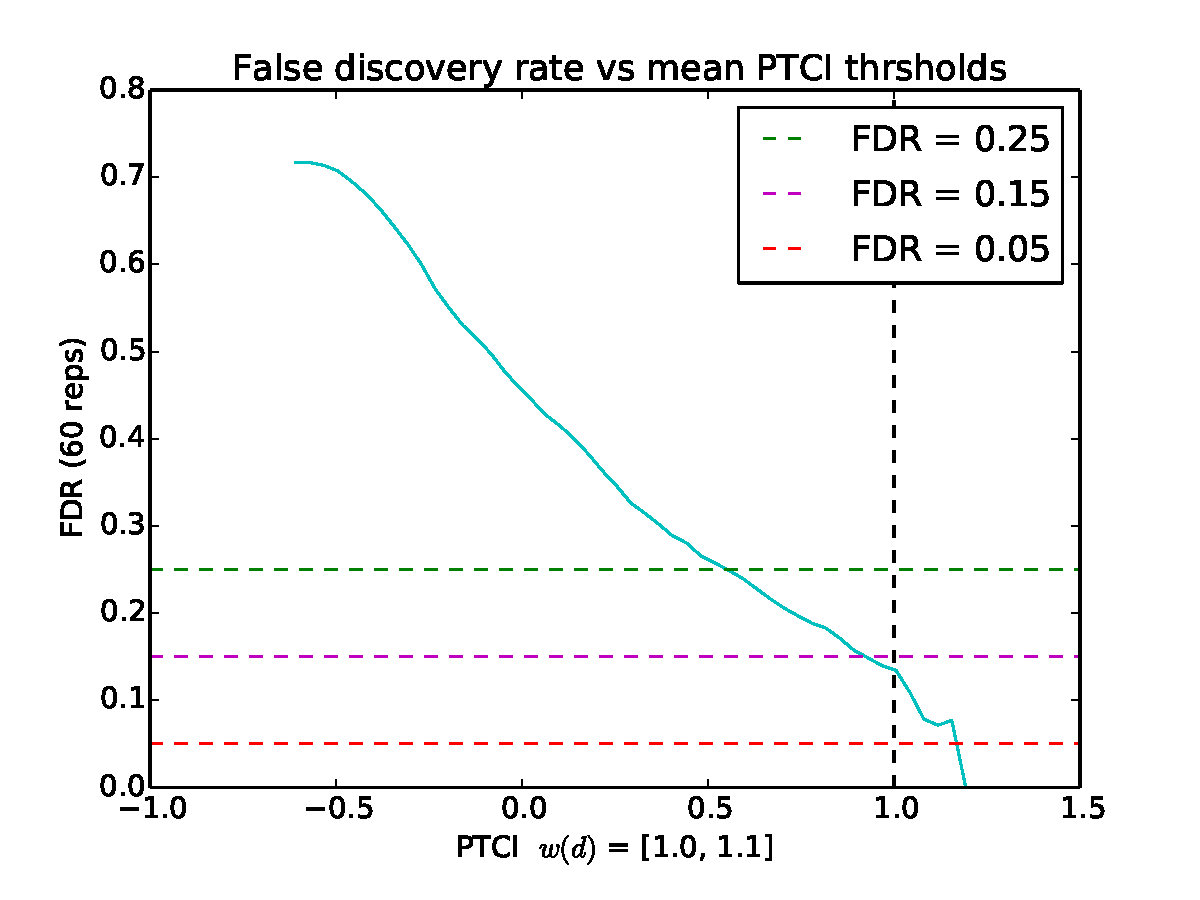
\includegraphics[width=.5\linewidth]{figures/figs/jaspar_insect_ptci_20130918_orthodb7/mean_ptci_fdr.pdf}}
% 
% 
\caption[Mean insect-PTCI results]{\sf \textbf{Mean PTCI results for the insect-\gls{TFBS} group}:\\
\textbf{(A)} Histogram of mean PTCI results vs null distributions.
\textbf{(B)} Reverse Cumulative histogram of mean PTCI results vs null distributions.
\textbf{(C)} False discover rate vs PTCI threshold.}
\label{fig:insect-mean-ptci-hists}
\end{figure}
%
\FDR\ estimation was used to determine a suitable \PTCI\ value to use as a threshold for further investigating particular 3-way 1:1 ortholog sets.
%
It was determined that in both \gls{TFBS} model data-sets a mean \PTCI\ threshold of 0.95 yielded an \FDR\ of approximately 15\% and maximized the number of genes for further classification (Figures \ref{fig:ecr-mean-ptci-hists-fdr} and \ref{fig:insect-mean-ptci-hists-fdr}).
%
This threshold produced 666 and 708 genes in the \PTCIi\ and \PTCIe\ sets, respectively.
%
The union of these gene-sets was 930 genes or 310 genes from each species.
%
The intersection was 444 or an overlap of 66\% of the \PTCIi\ genes and 62.7\% of the \PTCIe\ genes.
%
The unique proportion contributed by each set was 33\% and 37.3\%, respectively.

\paragraph*{Mean vs pairwise PTCI:}
Comparing the \FDR\ values of the pairwise- and mean-\PTCI\ scores at the 0.95 threshold reveals the impact of considering information from all 3-way 1:1 orthologs simultaneously rather than species-pair by species-pair (Figures \ref{fig:ecr-pair-ptci-hists-fdr} vs \ref{fig:ecr-mean-ptci-hists-fdr} and Figures \ref{fig:insect-pair-ptci-hists-fdr} vs \ref{fig:insect-mean-ptci-hists-fdr}).
%
The quality, as judged by \FDR, is strikingly improved by including the relationships of all three species weighted by their pairwise evolutionary distance: an improvement of approximately 30 percentage points in both cases.

\section{Characterization of results stage}
These results pertain to the third stage of the approach described in Chapter \ref{chap:3} (Figure \ref{fig:approach-chart}: \textit{blue box}).

\subsection{Functional annotations (before k-means clustering)}

Functional annotations were obtained for the 930 genes using \gls{Argot2} (Section \ref{chap:3-sec:characterization-of-results}).
%
%% How many of the 930 were assigned at least one annotation >= 200? --> 760 (Aa:253 ,Ag:254 , Cq:253 )
%% How many genes got better than 2000? --> 452 (Aa: 154, Ag:153 , Cq:145 )
Of these, 760 were assigned, by \gls{Argot2}, at least one annotation with a \gls{TS} greater than or equal to 200\footnote{This is the threshold that is suggested by the developers based on their in-house benchmarking \url{http://www.medcomp.medicina.unipd.it/Argot2/help/argot\_scores.php\#ts}} (\Aa: 253, \Ag: 254, \Cq: 253).
%
452 were assigned annotations with \glspl{TS} greater than or equal to 2000 (\Aa: 154, \Ag: 153, \Cq: 145).
%
This indicates that on the whole, most of the 930 genes produced by the \gls{gFunc} process were assigned annotations of a quality at least as stringent as used by the developers of \gls{Argot2}.

%%%%%%%%%%%%%%%%%%%%%

\subsection{K-means clustering}

K-means clustering ($k=23$) was applied to the 310 genes from \Ag\ to partition the 3-way 1:1 ortholog sets based on \gls{mAP} similarity.
%
\Ag\ was selected because it shares approximately equidistant evolutionary divergence to both other species.
%
Four of the resulting clusters were chosen for further characterization (Figure \ref{fig:23-clusters}: \textit{Cluster IDs 4, 6, 16, and 22}) because they have expression patterns that may be regulated by a noted pulse of \gls{20E} that occurs around 4h \gls{PBM}\footnote{See Section \ref{chap:3-sec:clustering-of-filtered-ortholog-sets} for more information.}.
%

\begin{landscape}

    \begin{figure}[h]
    \centering
    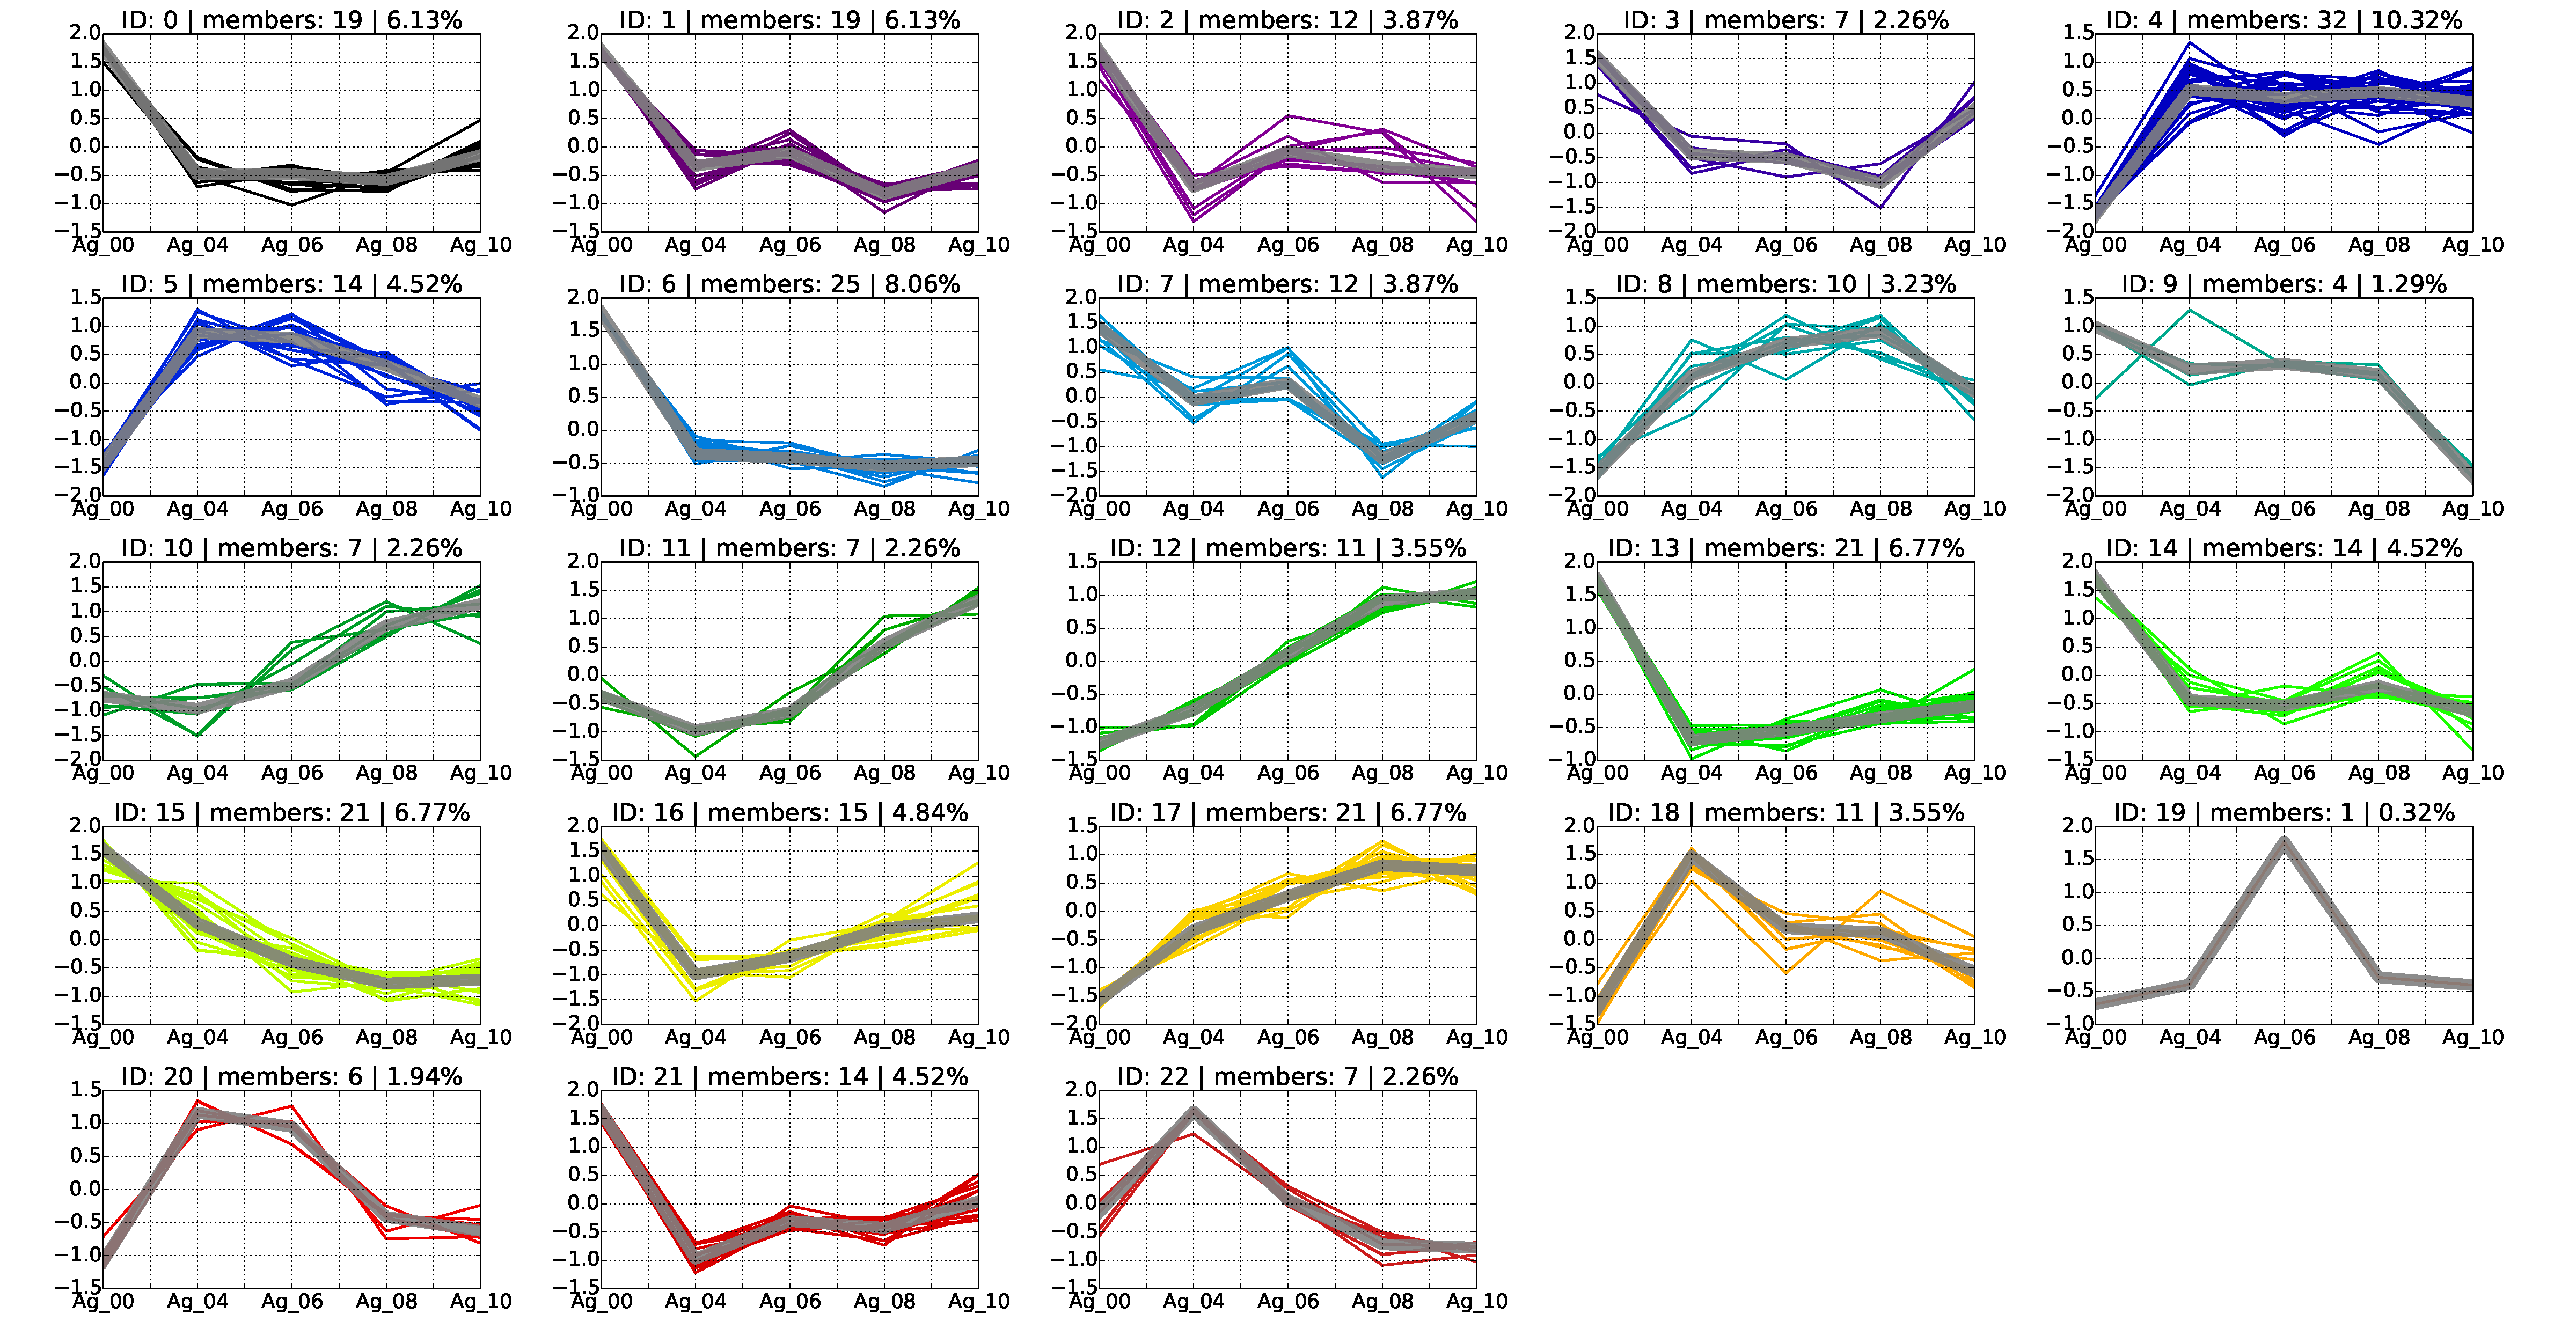
\includegraphics[width=\linewidth]{figures/figs/ecr_and_insects_ptci_20130918_orthodb7/23clusters_ptci_0_95_orthodb7.pdf}
    \caption[\Ag\ clustered abundance profiles]{\sf \textbf{\Ag\ clustered abundance profiles.} \\ 
    Clusters were generated using k-means clustering as implemented in Biopython version 1.62 \cite{Cock2009}.  Abundance profile data was log transformed after one FPKM was added to all data to remove zeros ($log_{10}(\mathrm{FPKM}+1)$).  K-means was then applied using the arithmetic mean as the center for cluster definition.  The data displayed here is the gene-wise standardization of the \textbf{raw} FPKM data such that each profile has mean = 0 and standard deviation = 1. Each median abundance profile is marked by a thick gray line. \textbf{Panel Titles} - ID: cluster identifier | members: number of genes in cluster | percentage of genes represented in all clusters. \textbf{Time Points} - \gls{NBF}, 4, 6, 8, 10 h \gls{PBM}.
}
    \label{fig:23-clusters}
    \end{figure}
    
\end{landscape}



\subsection{Highlighted clusters}

Clusters 4, 6, 16, and 22 were chosen for further characterization because they demonstrated patterns of mRNA accumulation that change sharply between \gls{NBF} and 4h \gls{PBM}.
%
Clusters 4 and 6 maintain similar \gls{FPKM} values for the remaining time points and are referred to as ``up after 4h'' (Figure \ref{fig:cluster4}) and ``down after 4h'' (Figure \ref{fig:cluster6}) respectively.
%
Clusters 16 and 22 follow the change in \gls{FPKM} at 4h \gls{PBM} by gradually trending back towards the original level of accumulation and are referred to as ``down at 4h'' (Figure \ref{fig:cluster16}) and ``up at 4h'' (Figure \ref{fig:cluster22}) respectively.
%
The interest in changes that focus on 4h \gls{PBM} stems from the description of a small but reproducible pulse of \gls{20E} that coincides with many important events which signal the switch from a \gls{JH} dominated signaling environment to one influenced by the lack of \gls{JH} and presence of \gls{20E}\footnote{See Discussion (Section \ref{chap:4-sec:discussion}) for more details.}

The cluster-specific functional annotation results included in the following sections, unless otherwise stated, represent the mean \gls{TS} for all occurrences of each term in the cluster-specific \gls{Argot2} results.
%
This provides an overview of which function and process gene ontology terms characterize the cluster as a whole rather than each individual gene which is too much information to include practically.
%
All original data and gene-term associations can be viewed via the IPython notebook files used to parse and organize the corresponding figures and tables that follow.
%
These are available at the supplementary figshare data repository associated with this dissertation\footnote{Files are located at \url{http://dx.doi.org/10.6084/m9.figshare.810442}. They are titled as ``ecr\_U\_insect\_ptci\_0\_95\_Exploring\_Profiles\_\textit{clsX}\_orthodb7.ipynb'' where \textit{clsX} defines the cluster number. Follow the instructions under the \textbf{Viewing IPython notebooks (ipynb files)} heading to explore the code, figures, and full tables.} \cite{Dunn2013dissSupl}.

\subsubsection{Cluster 4 (up after 4h)}

\paragraph*{General description:}

Cluster 4 is characterized by genes that have a median \gls{NBF} \gls{FPKM} of approximately 1.5 standard deviations \textit{below} the overall mean \gls{FPKM} followed by median \gls{FPKM} values between 0 and 0.5 standard deviations \textit{above} the overall mean \gls{FPKM} for the remainder of the time course (Figures \ref{fig:23-clusters} and \ref{fig:cluster4}).
%
This \gls{mAP} illustrates a rapid and sustained increase in mRNA abundance putatively triggered by the bloodfeeding stimulus.
%
\begin{figure}[p]
% 
\subcaptionbox{\label{fig:cluster4-Aa}}
{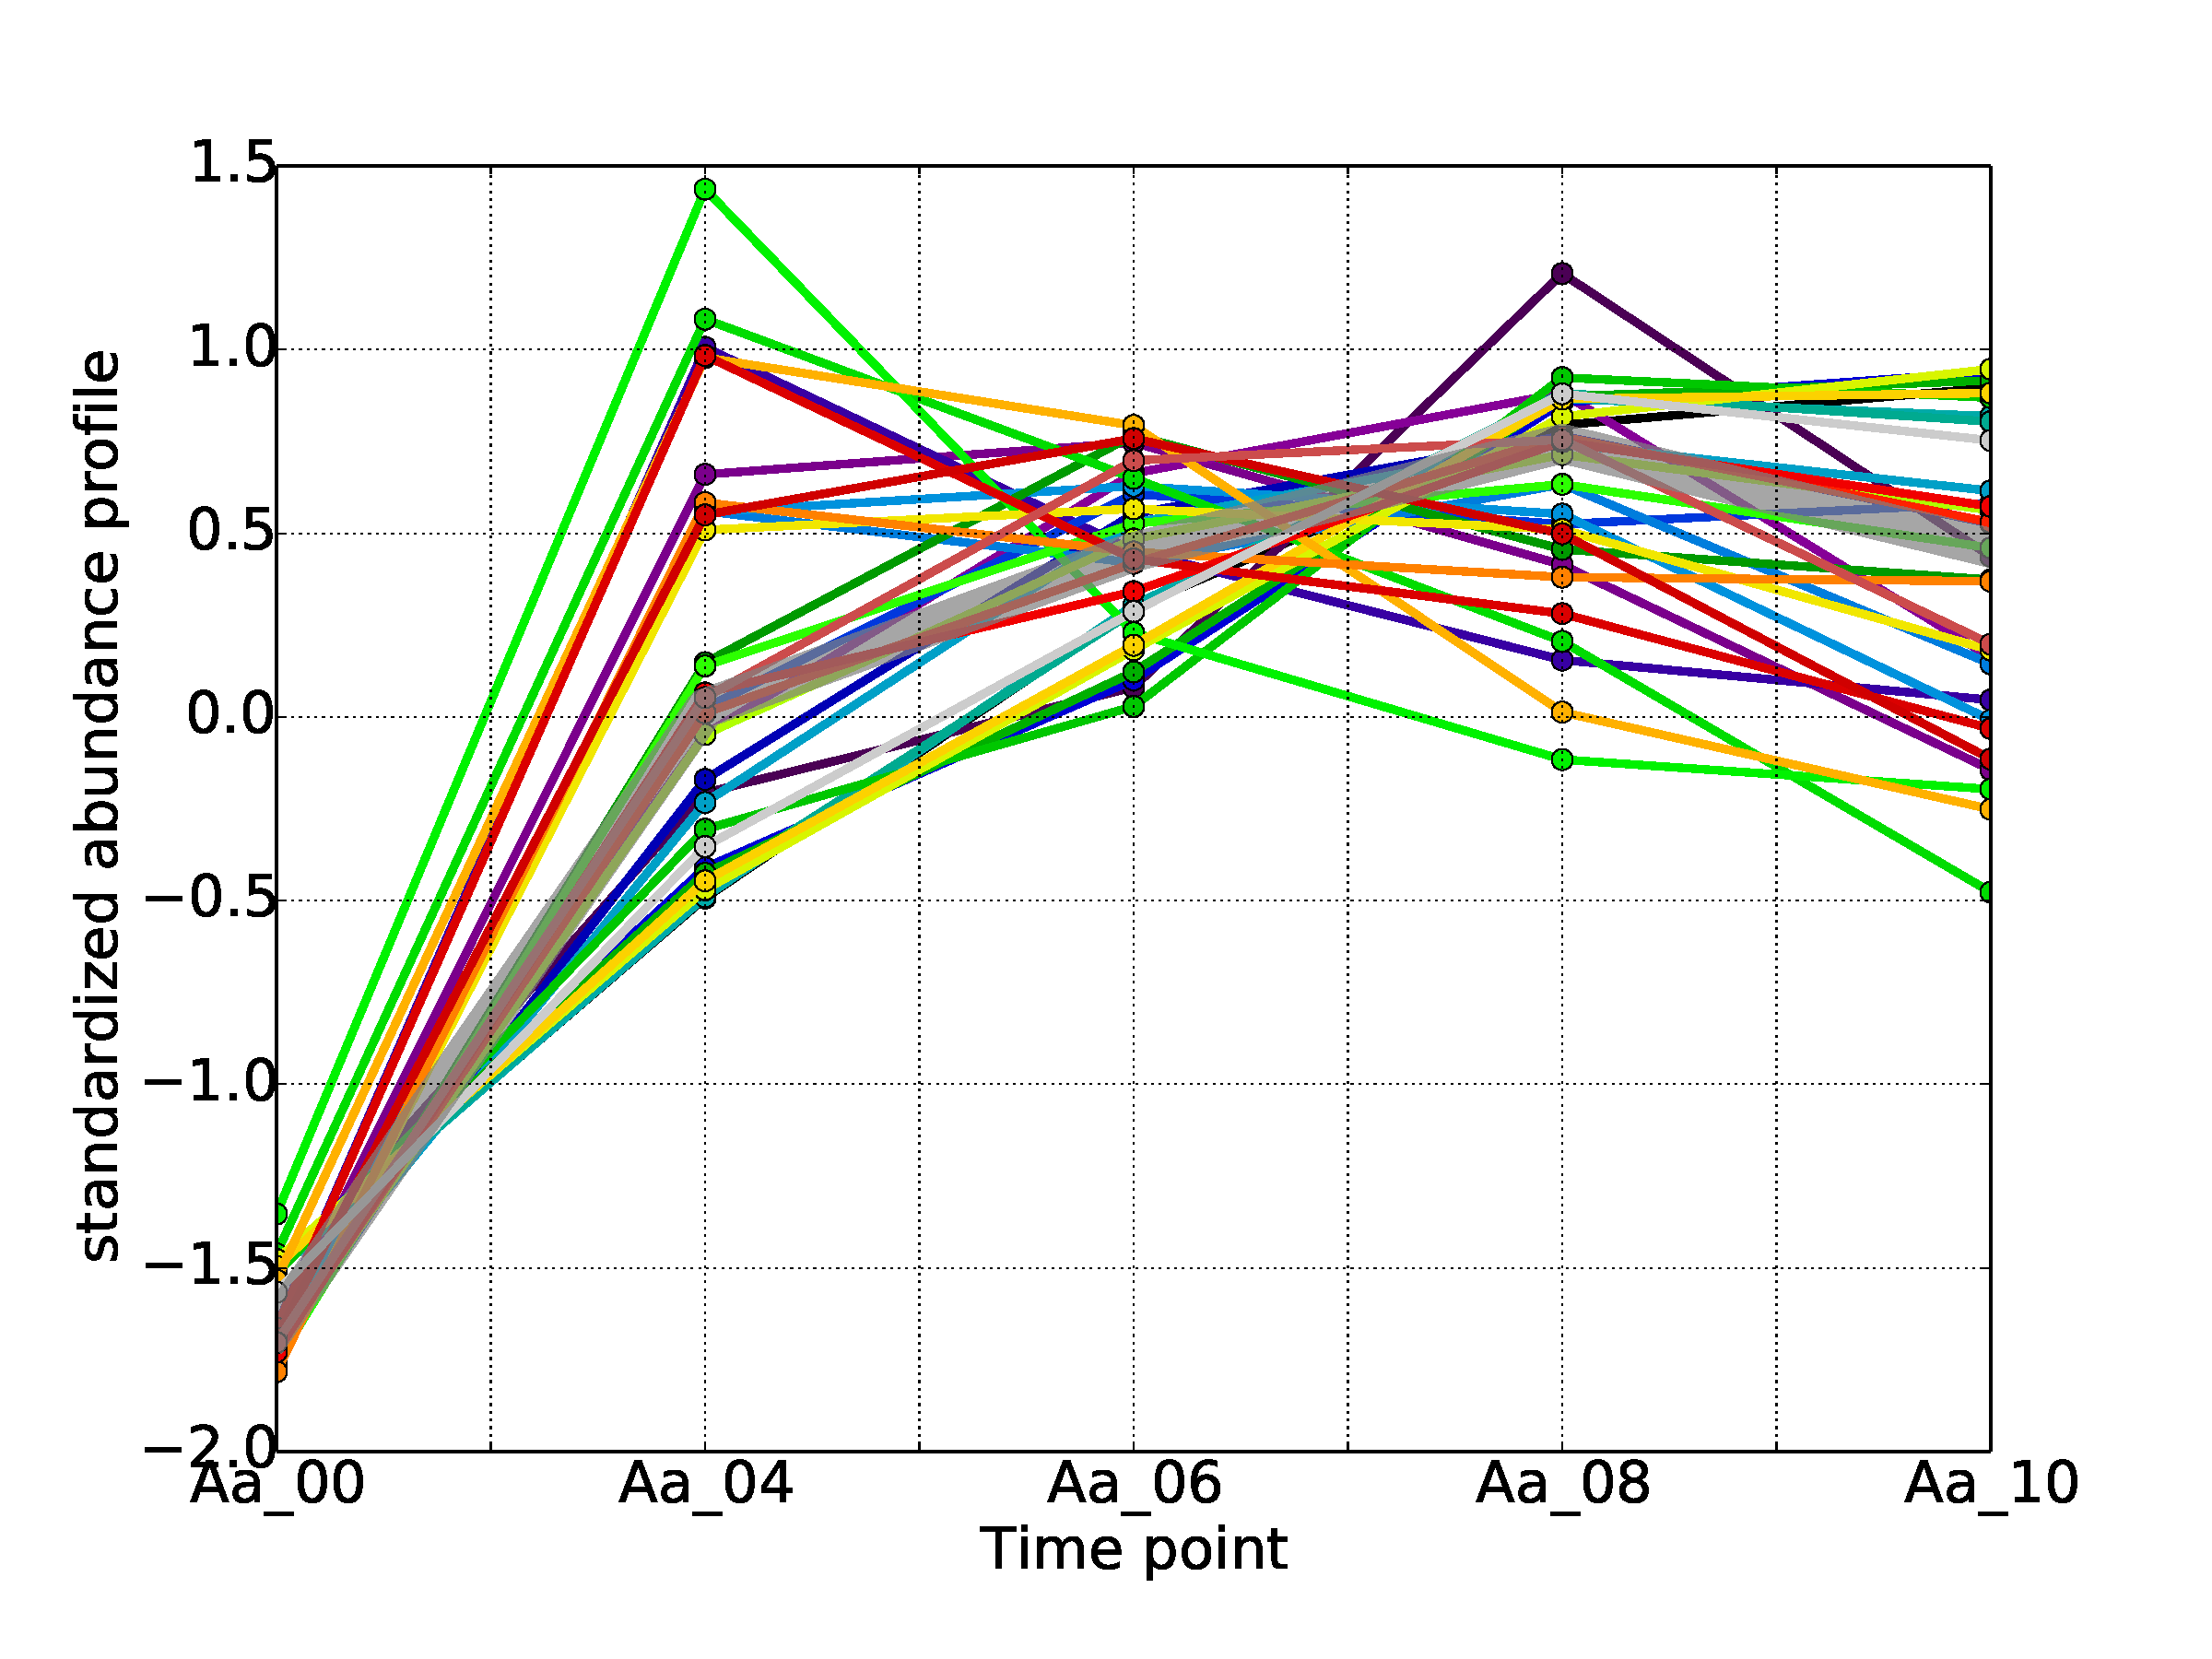
\includegraphics[width=.5\linewidth]{figures/figs/ecr_and_insects_ptci_20130918_orthodb7/upAfter4_gene_profiles_from_cummerbund/Aa_upAfter4_cls4_Ag_target_FPKMs_vb_orthos.pdf}}
%
\subcaptionbox{\label{fig:cluster4-Ag}}
{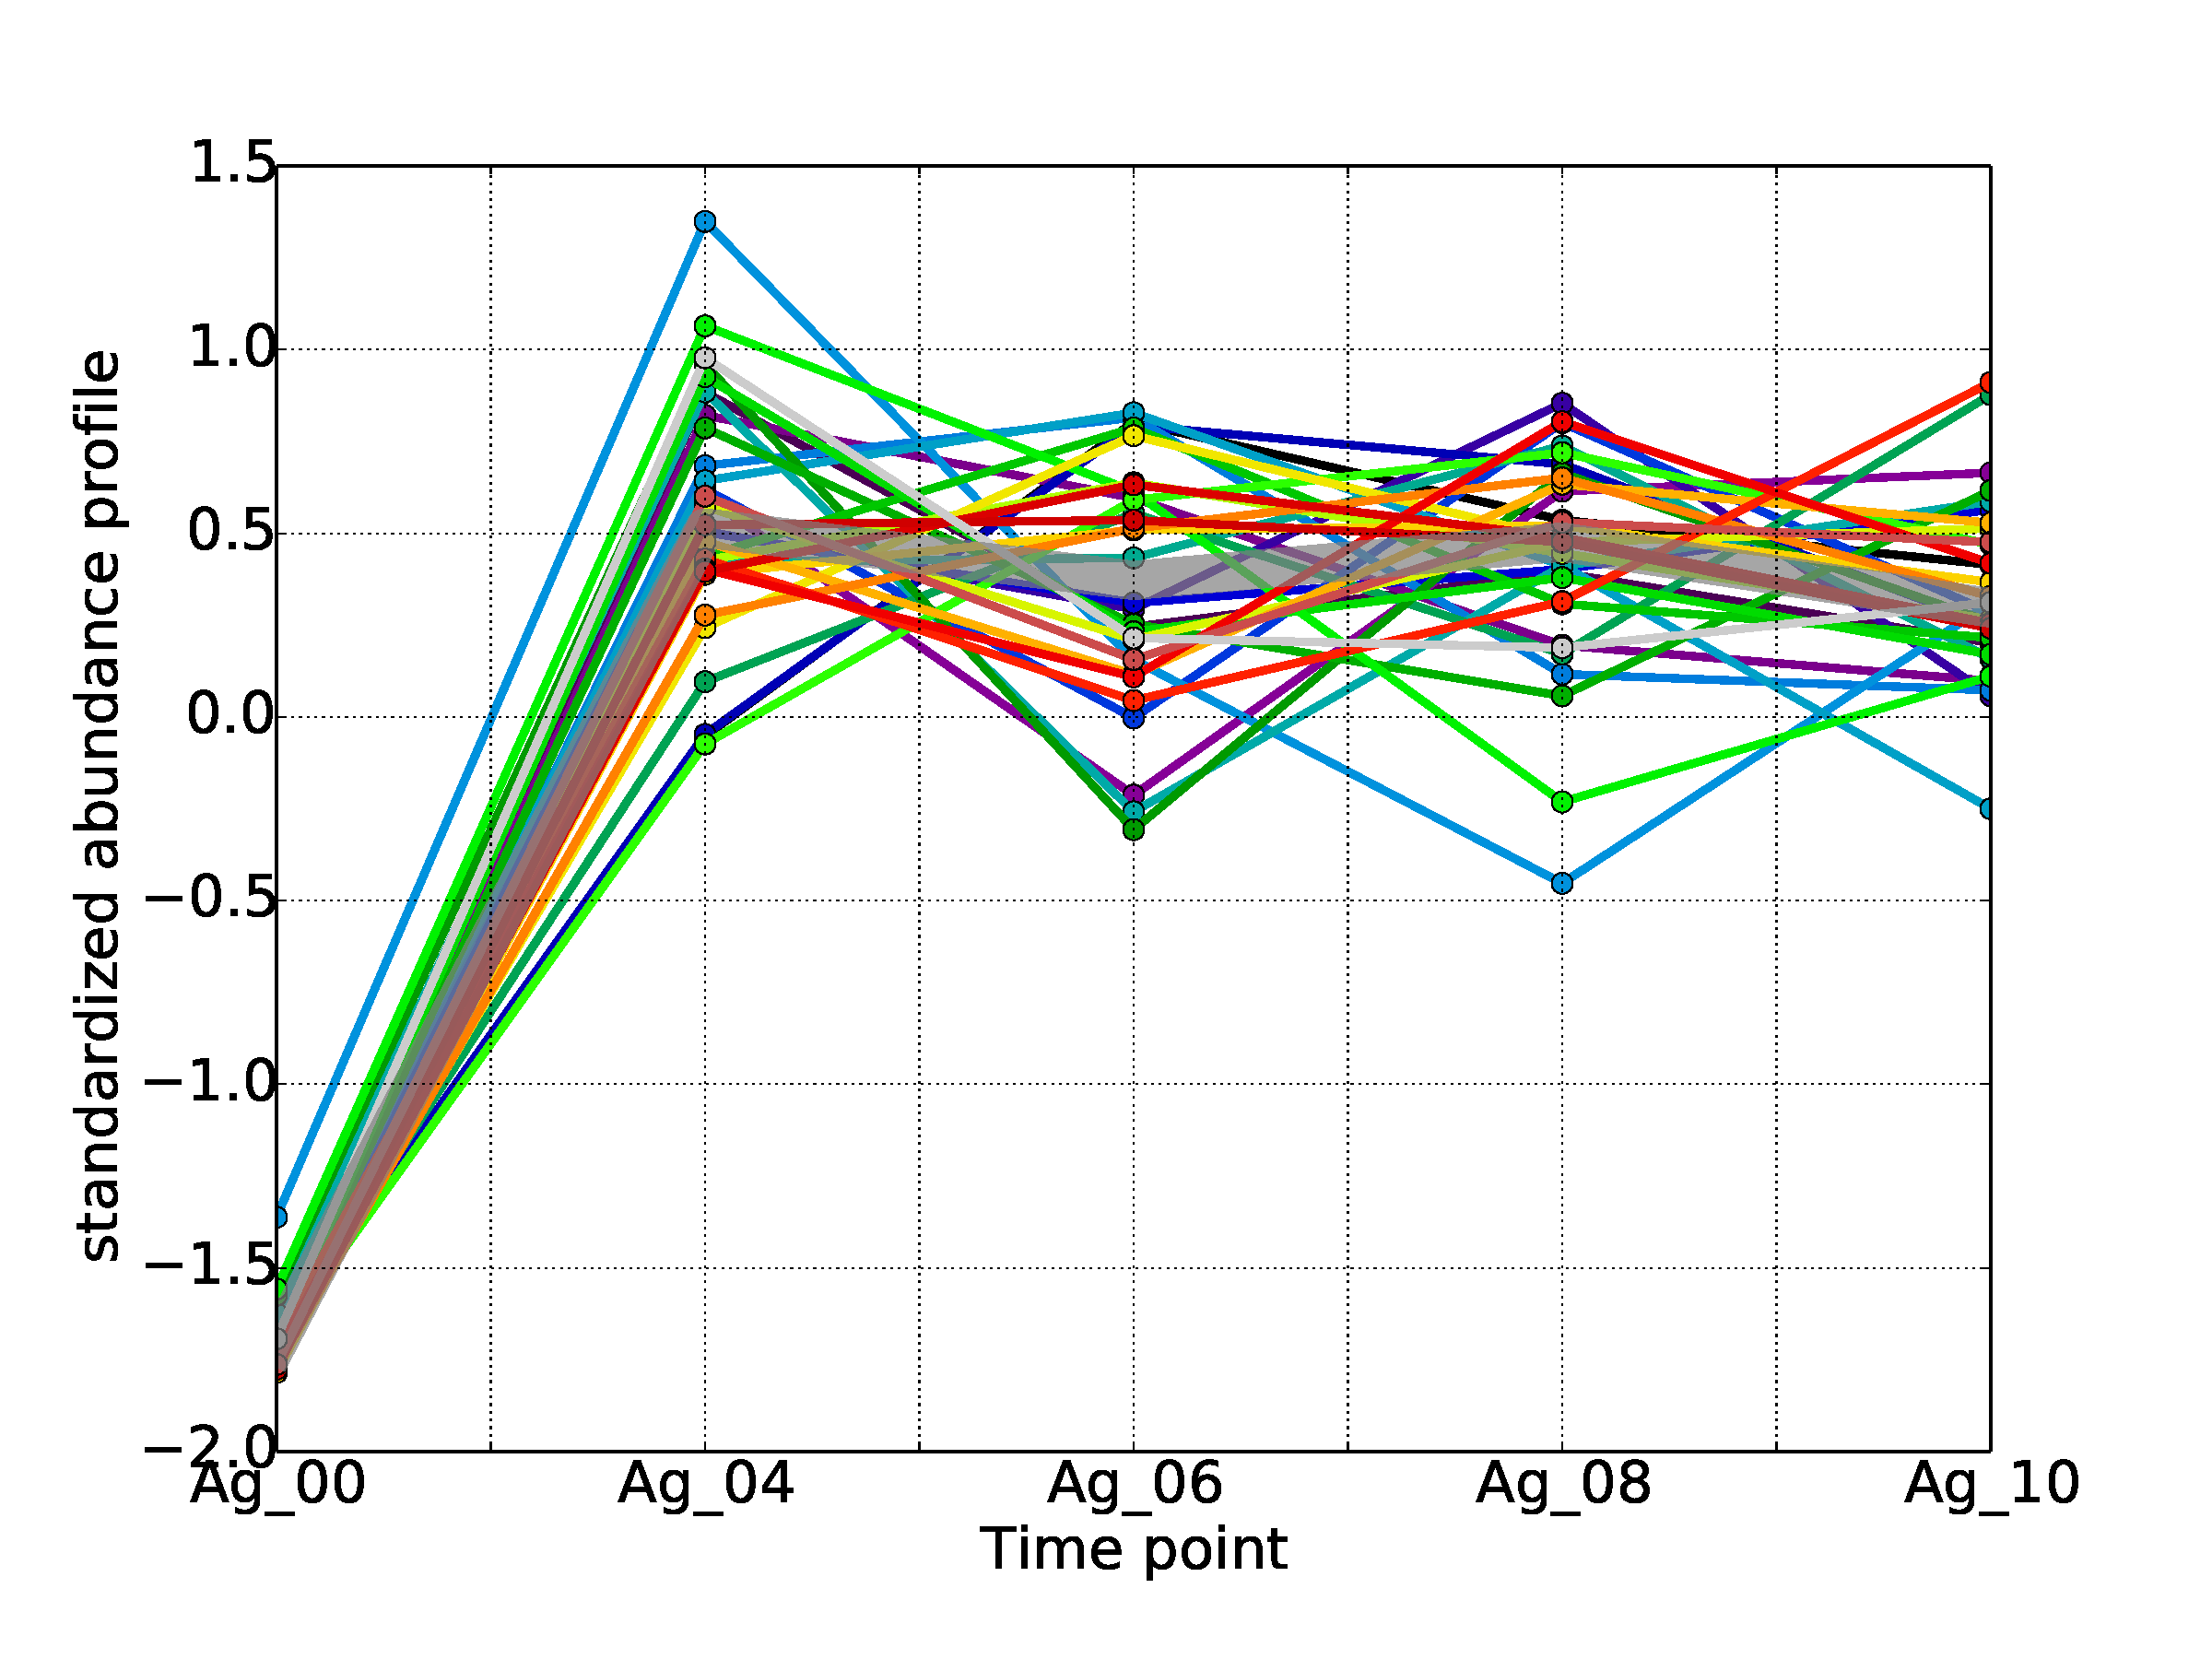
\includegraphics[width=.5\linewidth]{figures/figs/ecr_and_insects_ptci_20130918_orthodb7/upAfter4_gene_profiles_from_cummerbund/Ag_upAfter4_cls4_Ag_target_FPKMs_vb_orthos.pdf}}
%
\subcaptionbox{\label{fig:cluster4-Cq}}
{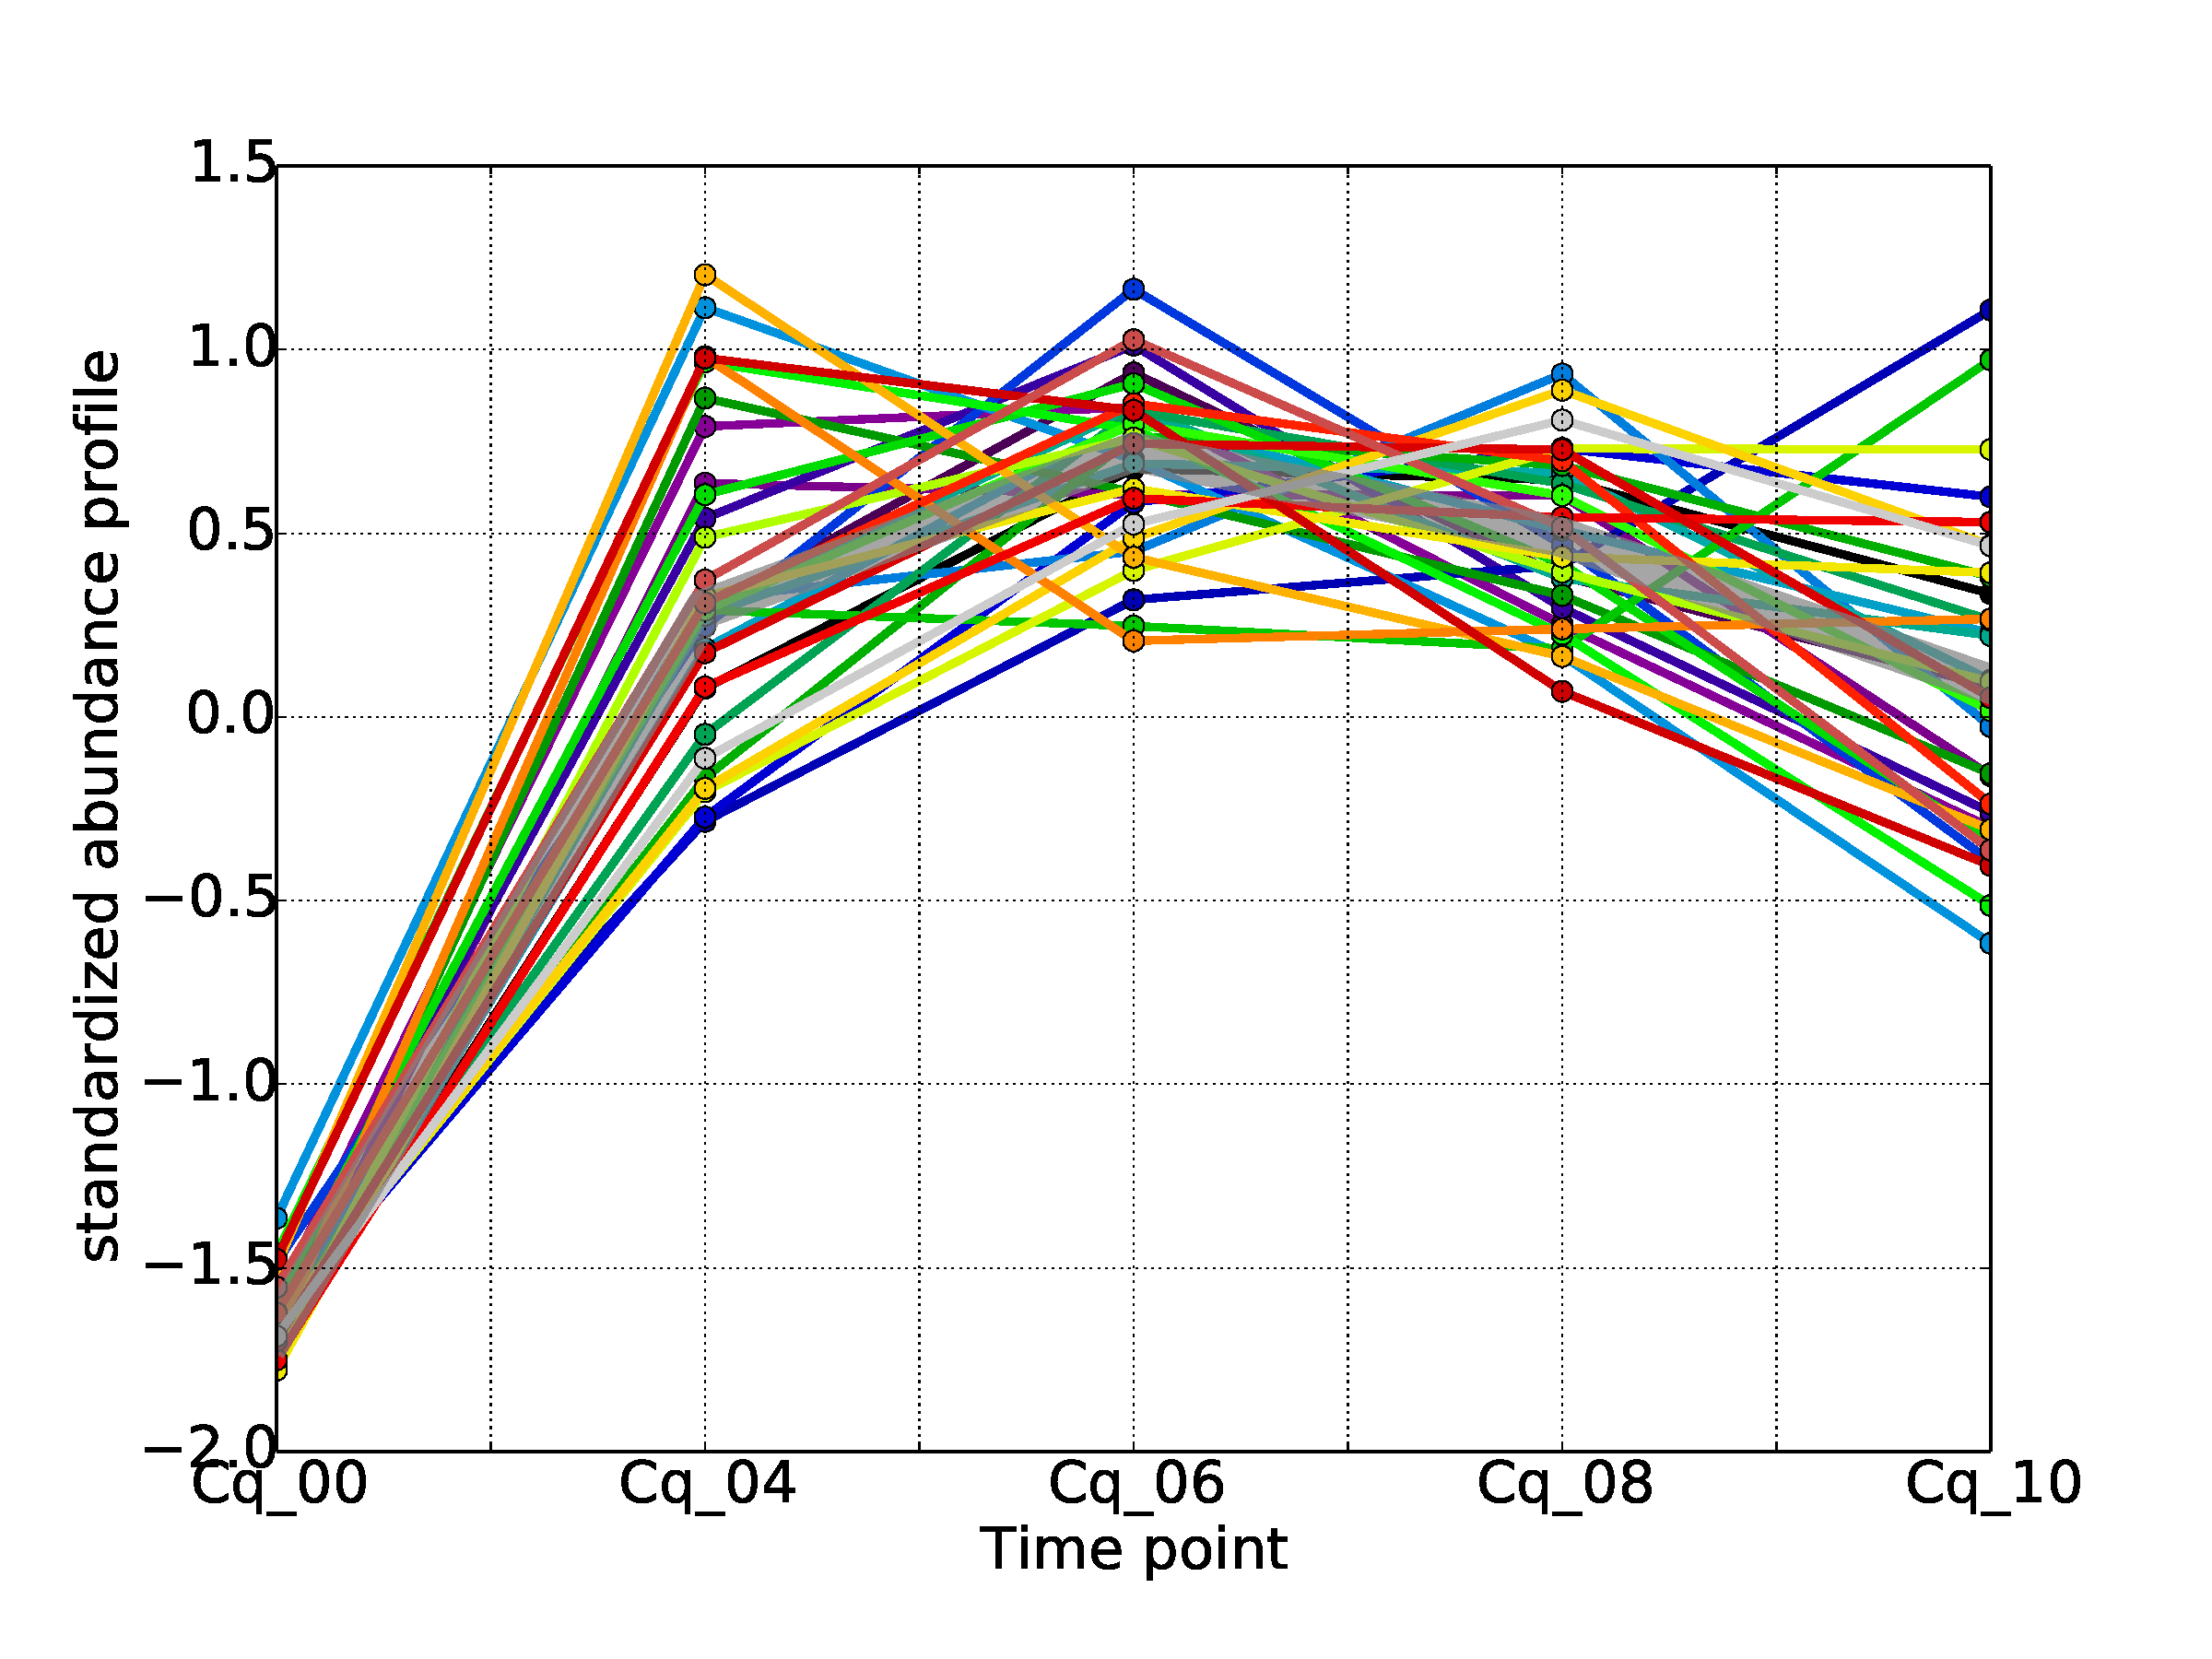
\includegraphics[width=.5\linewidth]{figures/figs/ecr_and_insects_ptci_20130918_orthodb7/upAfter4_gene_profiles_from_cummerbund/Cq_upAfter4_cls4_Ag_target_FPKMs_vb_orthos.pdf}}
% 
\caption[Orthologs of cluster 4]{\sf \textbf{Orthologs of cluster 4 (up after 4h):}\\
The same color scheme is used for each species which means that orthologs are given the same color in all three panels.
The thick, transparent gray line represents the median \gls{mAP} for the panel.
\textbf{(A)} \Aa.
\textbf{(B)} \Ag.
\textbf{(C)} \Cq.
}\label{fig:cluster4}
\end{figure}

\paragraph*{Functional annotations of cluster 4:}

% upregulation of translation/TOR
%	peptide quality control 
% active secretory pathways in both directions
% Metabolic activities

% Heme management
% midgut repair

The three main themes present in the \gls{Argot2} functional annotation terms for this cluster can be described as translation, secretory processes, and peptide metabolic activities.
%
Other supported activities include heme management and midgut repair (Tables \ref{tab:cls4-process} and \ref{tab:cls4-function}).
% Booktabs require to add \usepackage{booktabs} to your document preamble
\begin{table}[hp]
\begin{center} \sf
\begin{tabular}{p{.7\textwidth}r}
\toprule
\textbf{Name}                                                 & \textbf{Total Score (mean)} \\ \midrule
SRP-dependent cotranslational protein targeting to membrane   & 13254.87                    \\ % secretion / nutrient pathway
Golgi organization                                            & 7289.78                     \\ % secretion / nutrient pathway
glutamine biosynthetic process                                & 7056.26                     \\
bone development                                              & 6844.92                     \\ % #EXPLAIN #LOOKUP << LOOK HERE: http://pfam.sanger.ac.uk/family/PF09742 --> Functionally this protein might be involved in vesicle secretion or be an inter-cellular signalling protein or be a novel insulin receptor.[PMID 14504222] >>
ER to Golgi vesicle-mediated transport                        & 5914.05                     \\
heme biosynthetic process                                     & 5069.12                     \\ % bloodmeal
regulation of translational initiation                        & 4594.46                     \\ % translation/ TOR?
formation of translation preinitiation complex                & 4524.89                     \\ % translation/ TOR?
translational initiation                                      & 4288.82                     \\
translation                                                   & 3777.61                     \\
% positive regulation of GTPase activity                        & 3543.72                     \\
proteasome assembly                                           & 3326.44                     \\ % upregulated translation
porphyrin-containing compound biosynthetic process            & 3077.12                     \\ % #EXPLAIN #LOOKUP {{ferrochetalase}}
proton transport                                              & 2772.26                     \\ % digestion? endocytosis?
% ATP catabolic process                                         & 2642.02                     \\ % consumption of ATP / energy for proton transport?
proteolysis                                                   & 2453.58                     \\ % digestion
regulation of autophagy                                       & 2294.64                     \\ % change from starvation to nutrient excess
retrograde vesicle-mediated transport, Golgi to ER            & 2202.55                     \\
L-lysine catabolic process to acetyl-CoA via saccharopine     & 2148.61                     \\
vesicle fusion with Golgi apparatus                           & 2141.47                     \\
proteolysis involved in cellular protein catabolic process    & 1972.16                     \\
ubiquitin-dependent protein catabolic process                 & 1963.42                     \\
nitrogen compound metabolic process                           & 1885.16                     \\ % #EXPLAIN
ATP hydrolysis coupled proton transport                       & 1860.32                     \\ 
cell-cell adhesion                                            & 1774.89                     \\ % Midgut repair?
small GTPase mediated signal transduction                     & 1693.93                     \\
% response to drug                                              & 1507.48                     \\
% Golgi vesicle transport                                       & 1410.43                     \\
% intracellular protein transport                               & 1382.58                     \\
oligopeptide transport                                        & 1243.85                     \\
% cellular membrane fusion                                      & 1216.84                     \\
protein ubiquitination                                        & 1073.12                     \\
transmembrane transport                                       & 1025.68                     \\
vesicle-mediated transport                                    & 930.96                      \\
% protein transport                                             & 905.51                      \\
% mitotic prophase                                              & 897.77                      \\
% peptide transport                                             & 721.42                      \\
% transport                                                     & 657.84                      \\
% oocyte growth                                                 & 543.51                      \\ % endoplasmic reticulum organization and vesical trafficing (this gene known important in nurse cell folicle relationship) {{Protein jagunal}}
ion transport                                                 & 480.36                      \\
glycine biosynthetic process, by transamination of glyoxylate & 464.76                      \\
autophagy                                                     & 447.12                      \\
L-lysine catabolic process                                    & 417.84                      \\
lysine catabolic process                                      & 414.33                      \\
% oogenesis                                                     & 406.52                      \\
L-cysteine catabolic process                                  & 378.10                      \\
exocytosis                                                    & 294.15                      \\ % digestive secretion ? {{Protein jagunal}} endoplasmic reticulum organization and vesical trafficing
% cell adhesion                                                 & 286.17                      \\
cell differentiation                                          & 279.02                      \\ % midgut repair ?
detoxification of cadmium ion                                 & 262.31                      \\
% multicellular organismal development                          & 253.99                      \\
small molecule metabolic process                              & 253.25                      \\
metabolic process                                             & 235.09                      \\
cellular nitrogen compound metabolic process                  & 234.76                      \\
lysine biosynthetic process                                   & 207.74                      \\
cellular amino acid biosynthetic process                      & 200.81                      \\ \bottomrule                                                           
\end{tabular}
\end{center}

\caption[Cluster 4 top process GO terms]{\sf \textbf{Cluster 4 top process GO terms}}
\label{tab:cls4-process}
\end{table}
% Booktabs require to add \usepackage{booktabs} to your document preamble
\begin{table}[hp]
\begin{center} \sf
\begin{tabular}{p{.7\textwidth}r}
\toprule
\textbf{Name}                                                                                  & \textbf{Total Score (mean)} \\ \midrule
translation initiation factor activity                                                         & 18796.17                    \\ % translation/ TOR?
protein transporter activity                                                                   & 13663.10                    \\
signal recognition particle binding                                                            & 9157.88                     \\
endoplasmic reticulum signal peptide binding                                                   & 7943.20                     \\ % secretion 
Rab GDP-dissociation inhibitor activity                                                        & 7361.38                     \\
hydrolase activity, acting on acid anhydrides, catalyzing transmembrane movement of substances & 6647.91                     \\
hydrogen ion transmembrane transporter activity                                                & 6278.87                     \\
ferrochelatase activity                                                                        & 4990.12                     \\
GTP binding                                                                                    & 4006.06                     \\
%enzyme binding                                                                                 & 3697.54                     \\
saccharopine dehydrogenase (NAD+, L-glutamate-forming) activity                                & 3453.61                     \\
zinc ion binding                                                                               & 3215.15                     \\
glutamate-ammonia ligase activity                                                              & 2901.02                     \\
RNA binding                                                                                    & 2799.62                     \\
ATPase activity, coupled to transmembrane movement of substances                               & 2678.79                     \\
pyridoxal phosphate binding                                                                    & 2586.25                     \\
transporter activity                                                                           & 2044.78                     \\
saccharopine dehydrogenase (NADP+, L-lysine-forming) activity                                  & 1890.88                     \\
threonine-type endopeptidase activity                                                          & 1842.63                     \\
GTPase activator activity                                                                      & 1780.38                     \\
transaminase activity                                                                          & 1686.97                     \\
aminopeptidase activity                                                                        & 1592.00                     \\
endopeptidase activity                                                                         & 1546.38                     \\
nucleoside-triphosphatase activity                                                             & 1372.39                     \\
ATPase activity                                                                                & 1369.37                     \\
hydrolase activity                                                                             & 1352.33                     \\
lyase activity                                                                                 & 1299.81                     \\
ubiquitin-protein ligase activity                                                              & 1261.81                     \\
oxidoreductase activity                                                                        & 1237.14                     \\
nucleotide binding                                                                             & 1166.69                     \\
GTPase activity                                                                                & 1110.62                     \\
protein binding                                                                                & 1013.21                     \\
oligopeptide transporter activity                                                              & 927.01                      \\
symporter activity                                                                             & 915.24                      \\
ligase activity                                                                                & 870.70                      \\
metallopeptidase activity                                                                      & 809.99                      \\
metal ion binding                                                                              & 794.06                      \\
peptidase activity                                                                             & 792.59                      \\
proton-transporting ATPase activity, rotational mechanism                                      & 702.75                      \\
% ATP binding                                                                                    & 662.73                      \\
% catalytic activity                                                                             & 438.09                      \\
transferase activity                                                                           & 319.82                      \\
dipeptide transporter activity                                                                 & 217.58                      \\ \bottomrule
\end{tabular}
\end{center}

\caption[Cluster 4 (up after 4h) mean function GO terms]{\sf \textbf{Cluster 4 (up after 4h) mean function GO terms}}
\label{tab:cls4-function}
\end{table}

Representative terms from the ``process'' ontology domain that directly pertain to translation include (trailing parentheticals represent the mean \gls{TS}) SRP-dependent cotranslational protein targeting to membrane  (13254.87), regulation of translational initiation (4594.46), formation of translation preinitiation complex (4524.89), translational initiation (4288.82), and translation (3777.61).
%
In addition, other process-terms include activities expected to be up-regulated when translation is increasing include proteasome assembly (3326.44), ubiquitin-dependent protein catabolic process (1963.42), and protein ubiquitination (1073.12).
%
Similarly, the ``function'' ontology domain terms related to translation include translation initiation factor activity (18796.17), RNA binding (2799.62), transaminase activity (1686.97), and transferase activity (319.82).

Both process and function domain terms suggest an increase in secretory activity as well (anterograde and retrograde directions).
%
Process terms include Golgi organization (7289.78), ER to Golgi vesicle-mediated transport (5914.05), retrograde vesicle-mediated transport, Golgi to ER (2202.55), and vesicle fusion with Golgi apparatus (2141.47).
%
Complementary function terms are signal recognition particle binding (9157.88) and endoplasmic reticulum signal peptide binding (7943.20).

A major difference between the nutrients available to female mosquitoes when bloodfeeding versus sugarfeeding (\gls{NBF} sample) is the abundance of protein.
%
The increase in transcription of genes that encode products related to metabolizing peptides is evident in these data as well.
%
For example, proteolysis (2453.58), proteolysis involved in cellular protein catabolic process (1972.16), L-lysine catabolic process (417.84), lysine catabolic process (414.33), and L-cysteine catabolic process (378.10) are represented in the process domain terms, while threonine-type endopeptidase activity (1842.63), aminopeptidase activity (1592.00), endopeptidase activity (1546.38), and peptidase activity (792.59) are examples from the function domain.

Other notable sets of functional annotations for cluster 4 include a set that involves heme management (heme biosynthetic process [5069.12], porphyrin-containing compound biosynthetic process [3077.12], and ferrochelatase activity [4990.12]) and a set that may be involved in cellular repair of the midgut (cell-cell adhesion [1774.89], autophagy [447.12], and cell differentiation [279.02]).
%
The heme management terms all stem from the AAEL005415-AGAP003719-CPIJ008006 ortholog-set.
%
These are ferrochelatase enzymes.
%
Ferrochelatase catalyzes the final step of heme biosynthesis, insertion of the iron atom into the porphyrin ring \cite{Layer2010}.
%



% \paragraph*{\glspl{mAP} between species:}
% \lipsum[3]





\subsubsection{Cluster 6 (down after 4h)}

\paragraph*{General description:}

Cluster 6 is characterized by genes that have a median \gls{NBF} \gls{FPKM} of approximately 1.5 standard deviations \textit{above} the overall mean \gls{FPKM} and median \gls{FPKM} values of approximately 0.5 standard deviations \textit{below} the overall mean \gls{FPKM} for the remainder of the time course (Figures \ref{fig:23-clusters} and \ref{fig:cluster6}).
%
This \gls{mAP} illustrates a rapid and sustained decrease in mRNA abundance following bloodfeeding.
%

\begin{figure}[hp]
% 
\subcaptionbox{\label{fig:cluster6-Aa}}
{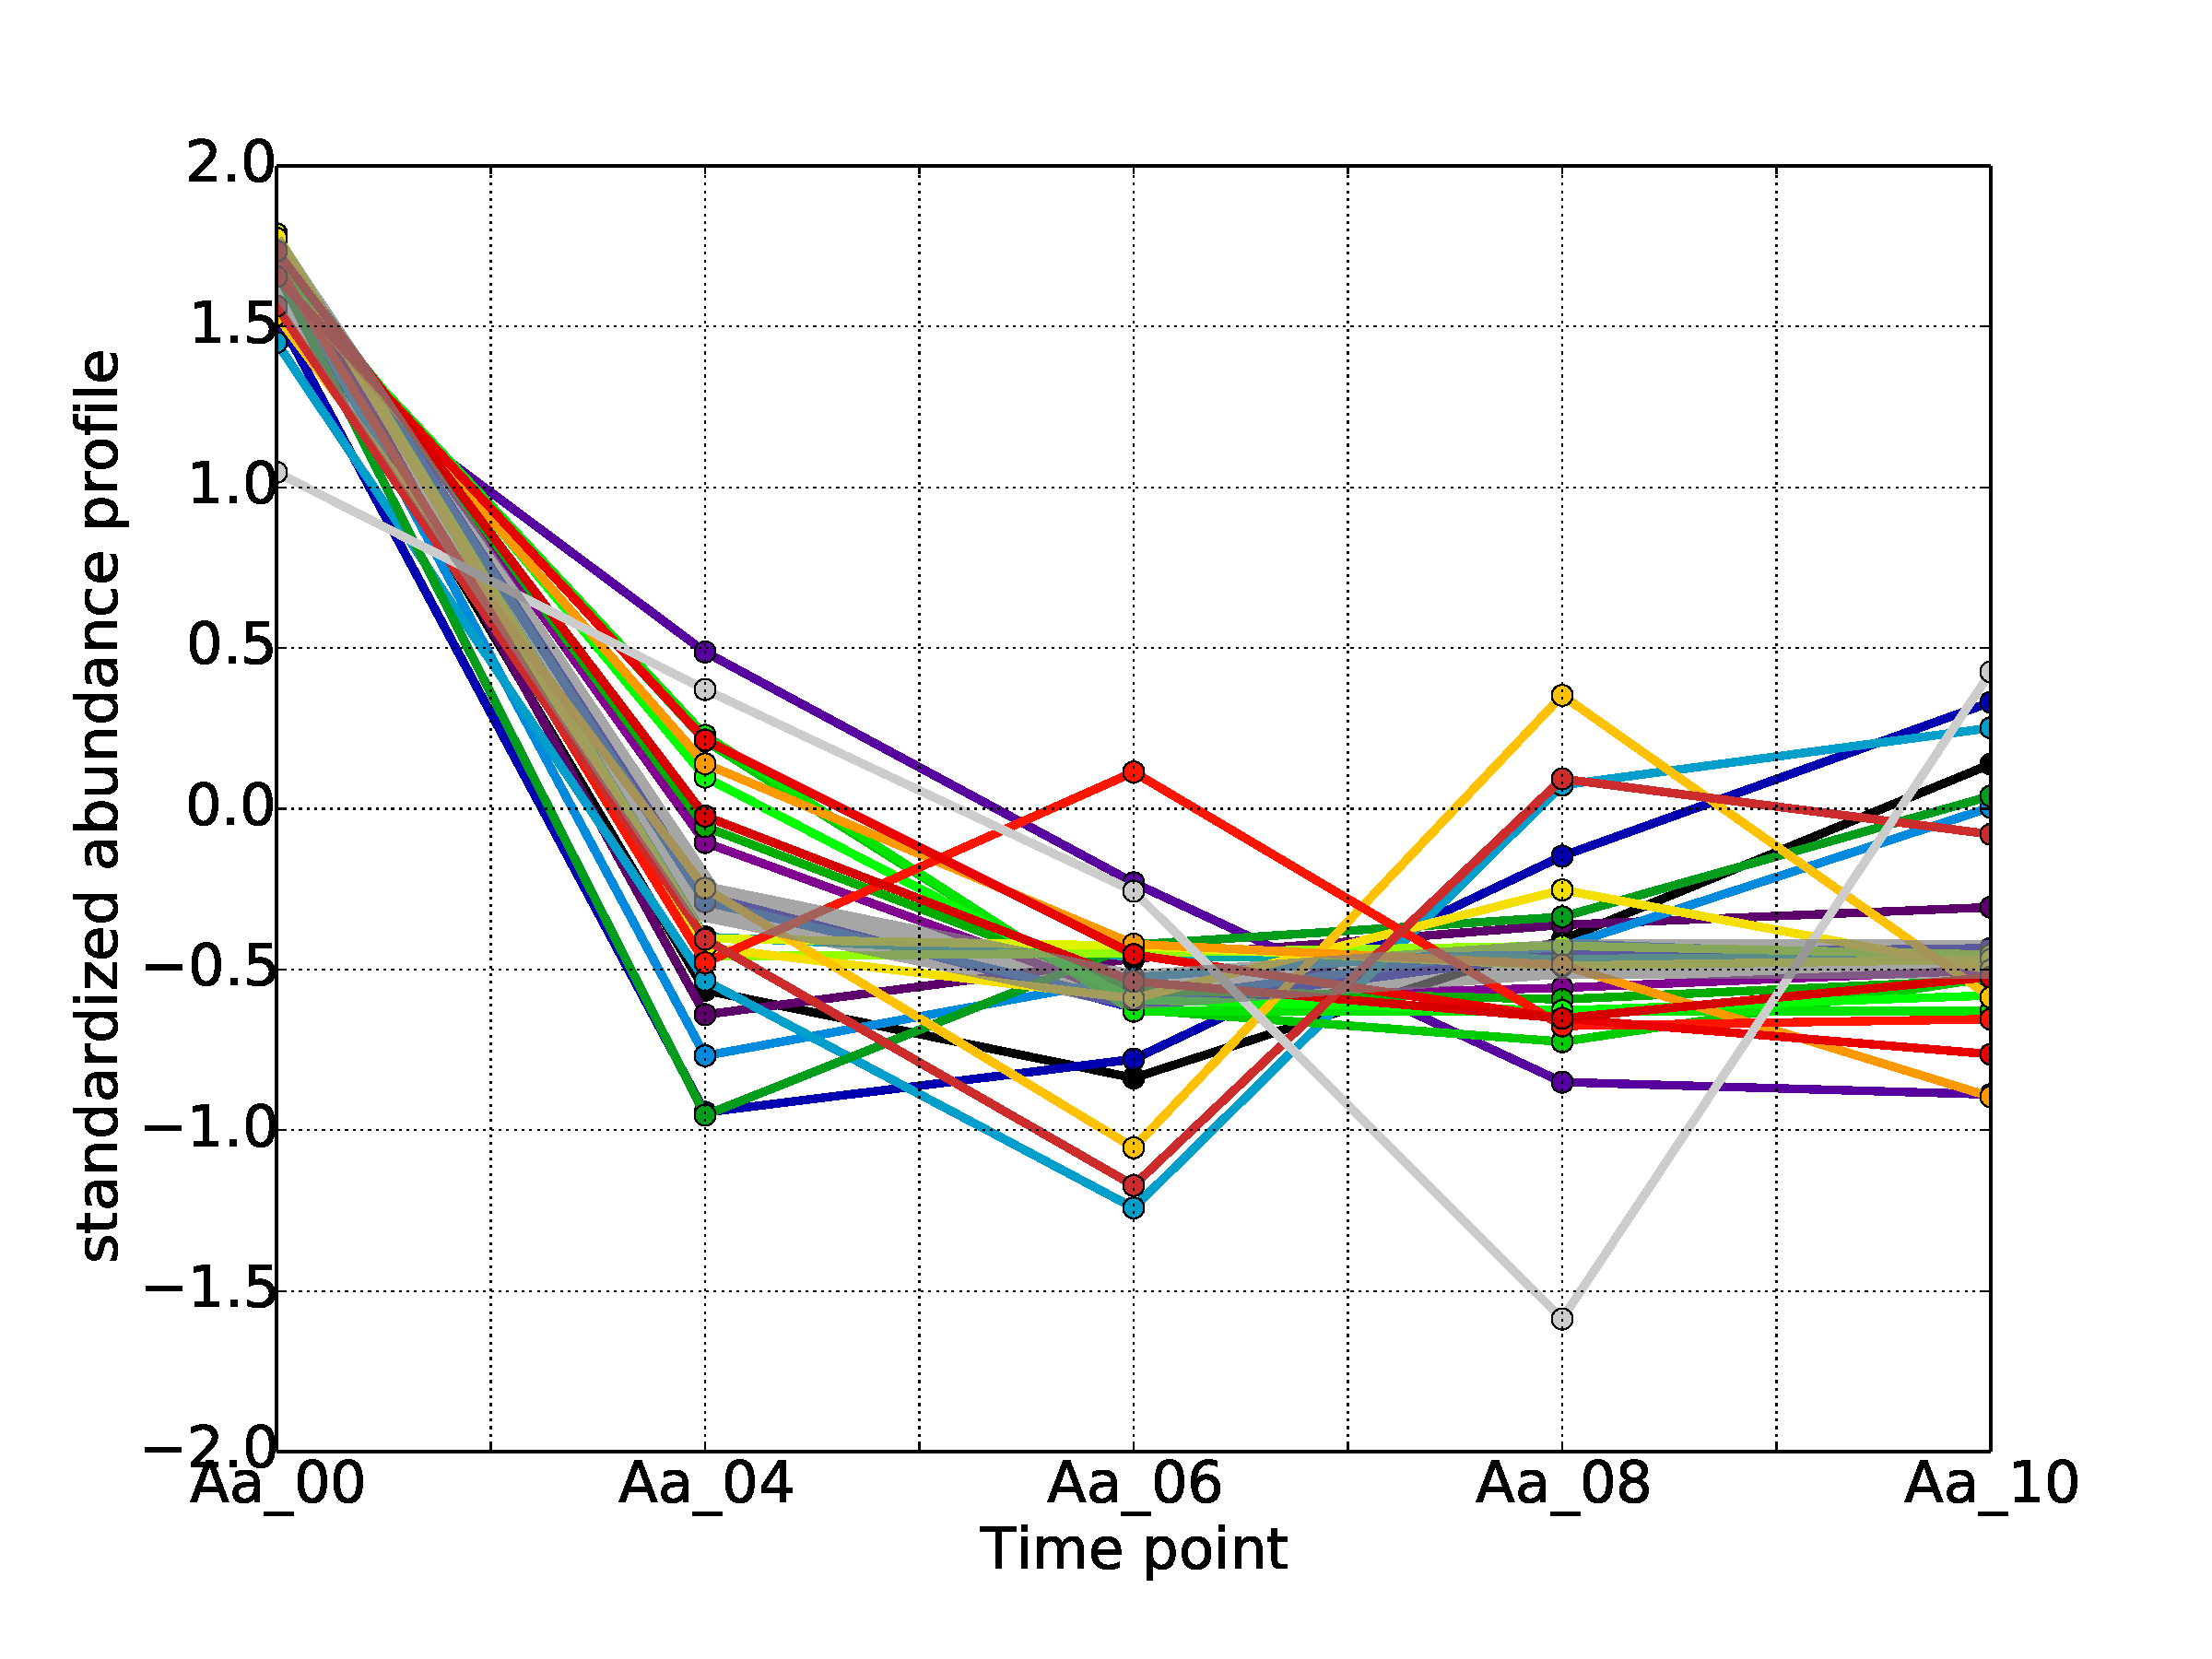
\includegraphics[width=.5\linewidth]{figures/figs/ecr_and_insects_ptci_20130918_orthodb7/downAfter4_gene_profiles_from_cummerbund/Aa_downAfter4_cls6_Ag_target_FPKMs_vb_orthos.pdf}}
%
\subcaptionbox{\label{fig:cluster6-Ag}}
{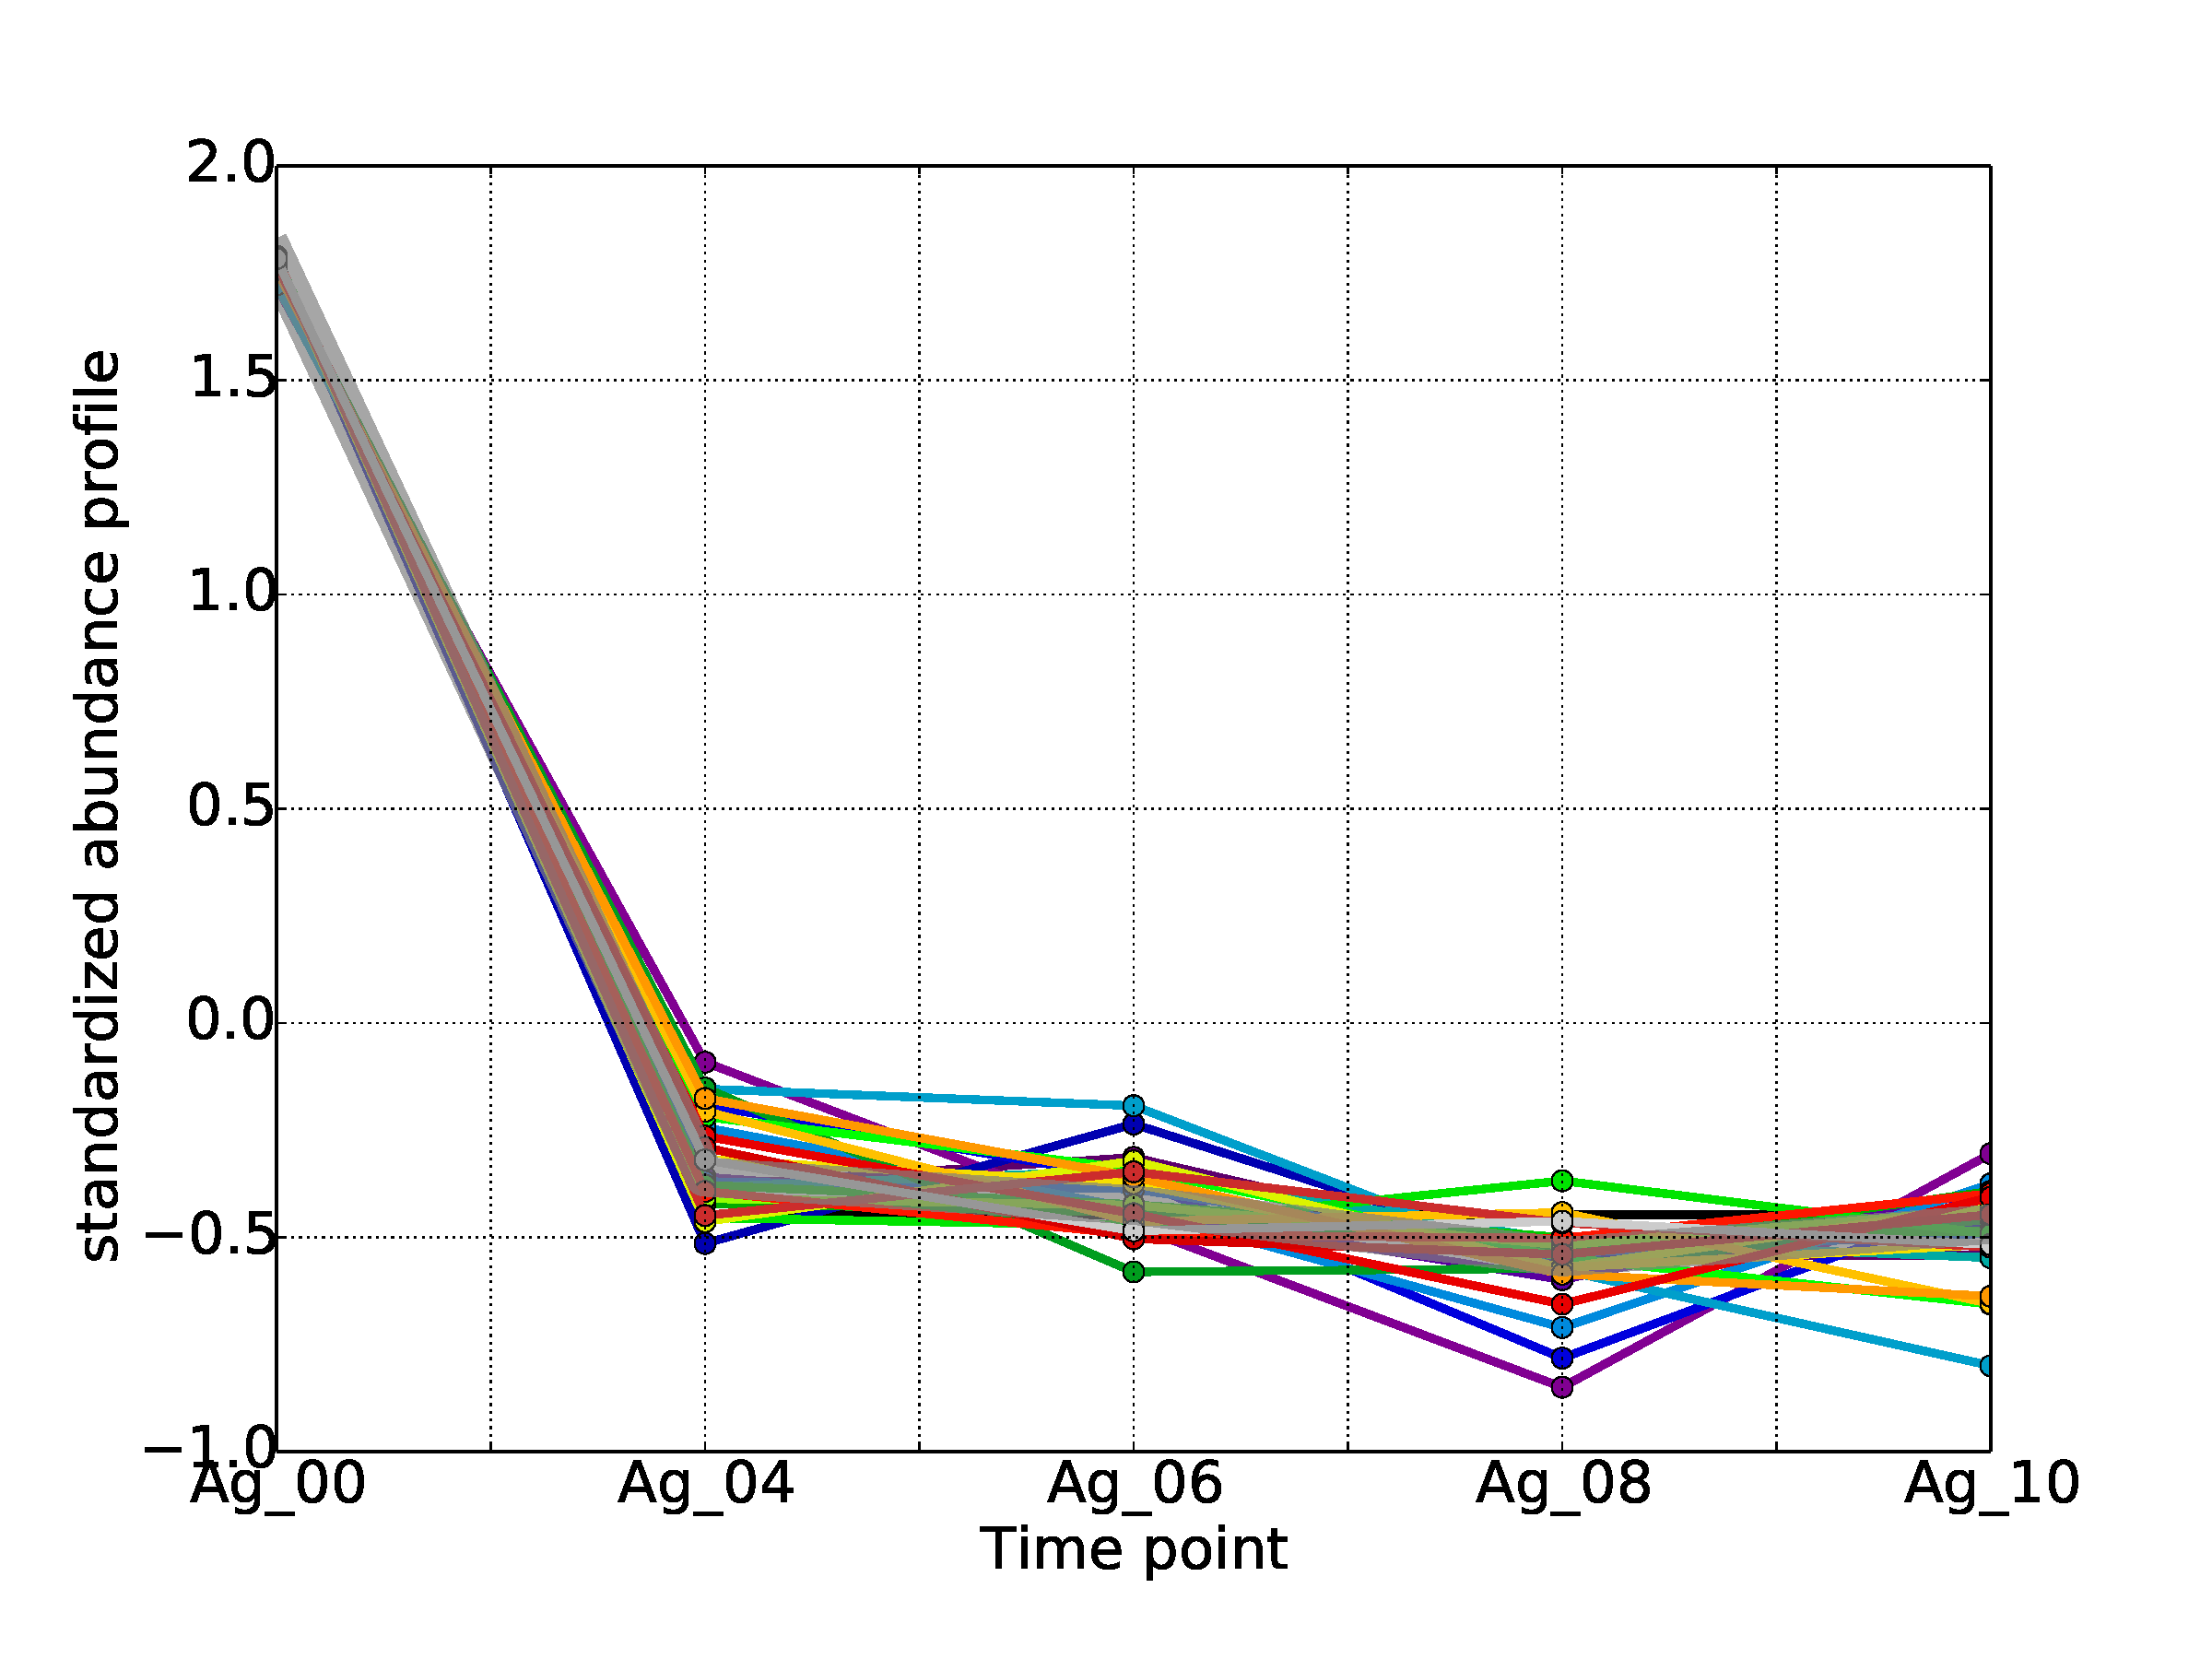
\includegraphics[width=.5\linewidth]{figures/figs/ecr_and_insects_ptci_20130918_orthodb7/downAfter4_gene_profiles_from_cummerbund/Ag_downAfter4_cls6_Ag_target_FPKMs_vb_orthos.pdf}}
%
\subcaptionbox{\label{fig:cluster6-Cq}}
{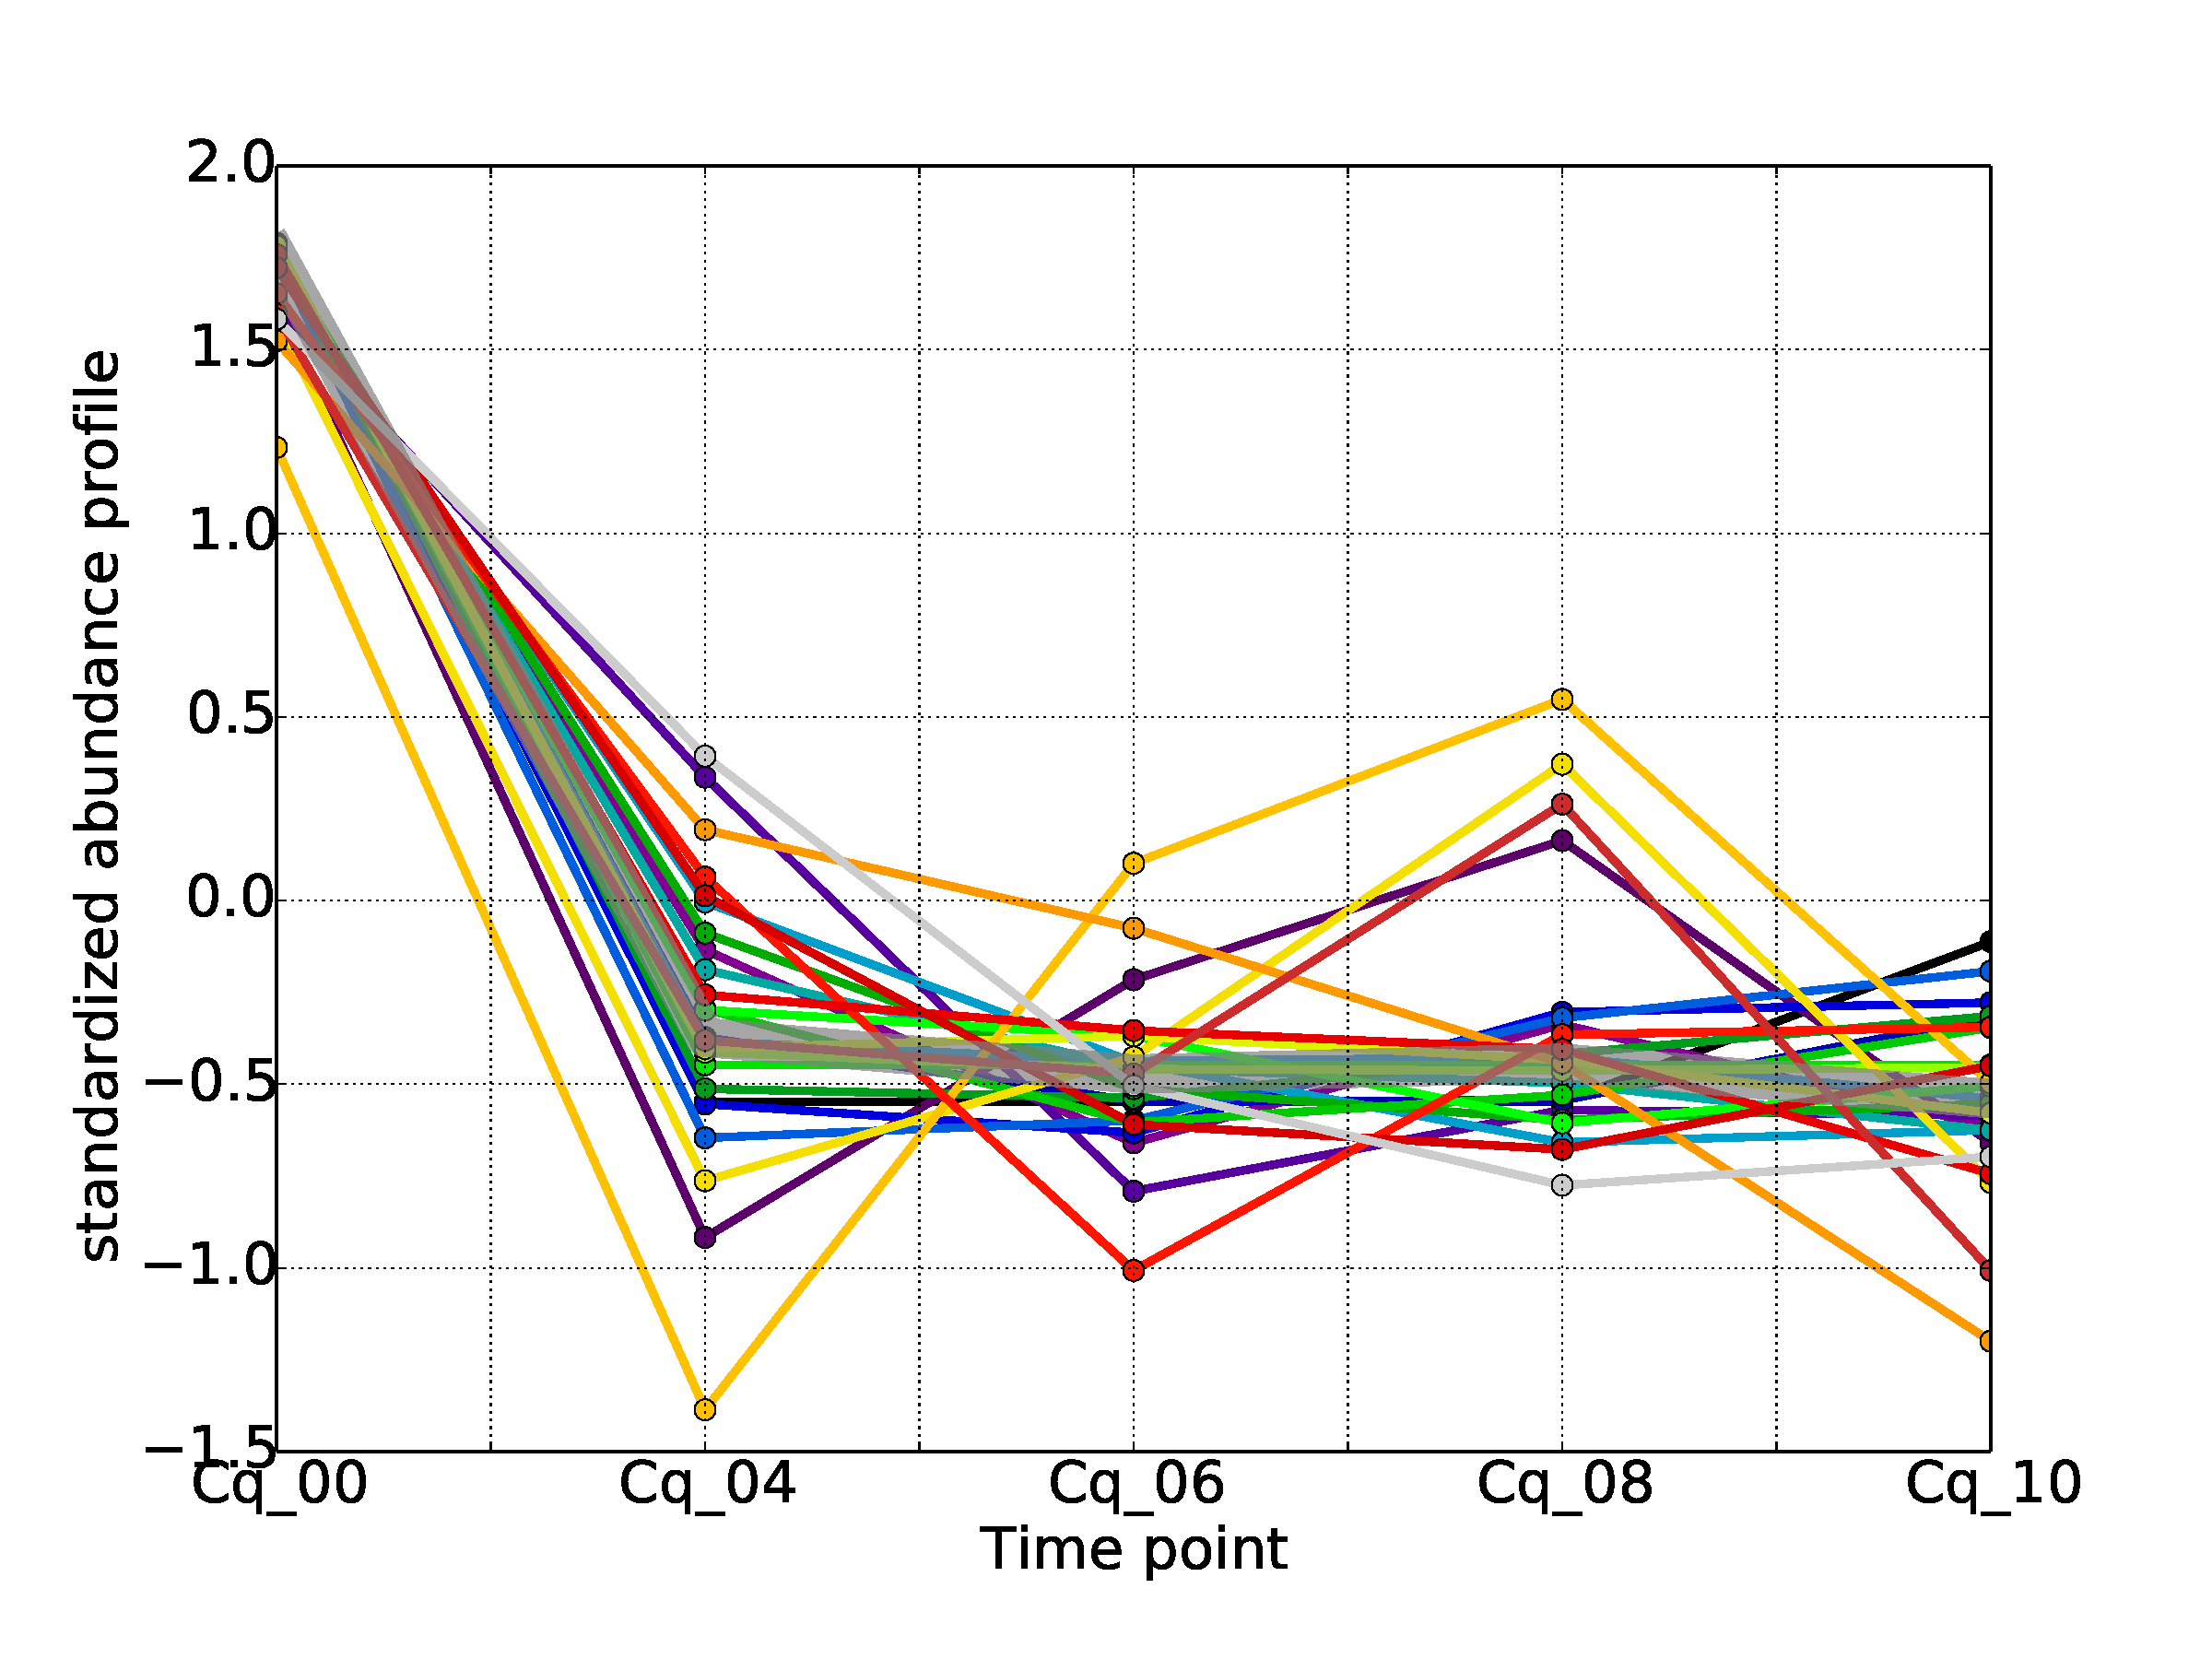
\includegraphics[width=.5\linewidth]{figures/figs/ecr_and_insects_ptci_20130918_orthodb7/downAfter4_gene_profiles_from_cummerbund/Cq_downAfter4_cls6_Ag_target_FPKMs_vb_orthos.pdf}}
% 
\caption[Orthologs of cluster 6]{\sf \textbf{Orthologs of cluster 6 (down after 4h):}\\
The same color scheme is used for each species which means that orthologs are given the same color in all three panels.
The thick, transparent gray line represents the median \gls{mAP} for the panel.
\textbf{(A)} \Aa.
\textbf{(B)} \Ag.
\textbf{(C)} \Cq.
}\label{fig:cluster6}
\end{figure}


\paragraph*{Functional annotations of cluster 6:}

% downregulation of transcription factors
% translation elongation
% signaling
% Heme management


% transcription factors
%	X AGAP002238:AAEL010222CPIJ008350 {GATA-type}
%	x AAEL009171:CPIJ001396:AGAP003726 {ortholog to Dmel bZIP family. CREBRF subfamily}
%	x CPIJ004057:AAEL009114:AGAP004050 {Doublesex}
%	x CPIJ014945:AAEL002062:AGAP005661 {Ftz-f1}
%	x AAEL001361:AGAP006990:CPIJ002241 {Bap 170 }
%	x CPIJ005607:AAEL005452:AGAP010201 {ortholog to Dmel crp}


Possible themes regarding the functional annotation terms for cluster 6 are down-regulation of certain transcription factors, signaling molecules, and heme management (Tables \ref{tab:cls6-process} and \ref{tab:cls6-function}).
% Booktabs require to add \usepackage{booktabs} to your document preamble
\begin{table}[hp]
\begin{center} \sf
\begin{tabular}{p{.7\textwidth}r}
\toprule
\textbf{Name}                                                           & \textbf{Total Score (mean)} \\ \midrule
Mo-molybdopterin cofactor biosynthetic process                          & 7762.64                     \\ % #LOOKUP
GTP catabolic process                                                   & 5712.72                     \\
translational elongation                                                & 3558.74                     \\
heme biosynthetic process                                               & 2615.06                     \\ % heme managment
glutamate biosynthetic process                                          & 2418.17                     \\
protein export from nucleus                                             & 2157.87                     \\
translation                                                             & 1962.19                     \\ % translation
cellular amino acid biosynthetic process                                & 1737.45                     \\
sex differentiation                                                     & 1549.60                     \\ % #EXPLAIN this is DBX
nuclear-transcribed mRNA catabolic process, nonsense-mediated decay     & 1190.98                     \\ % #LOOKUP
biosynthetic process                                                    & 1116.03                     \\
regulation of cyclin-dependent protein serine/threonine kinase activity & 950.21                      \\ % #LOOKUP CyclinT
cell adhesion                                                           & 938.98                      \\
intracellular protein transport                                         & 853.03                      \\
glutamine metabolic process                                             & 826.49                      \\
steroid hormone mediated signaling pathway                              & 779.04                      \\ % #LOOKUP (AGAP005661:AAEL002062:CPIJ014945 Ftz transcription factor)
protoporphyrinogen IX biosynthetic process                              & 769.19                      \\ % #LOOKUP Heme Biosynth
regulation of transcription, DNA-dependent                              & 760.48                      \\ 
nitrogen compound metabolic process                                     & 726.25                      \\
rRNA processing                                                         & 660.29                      \\
SRP-dependent cotranslational protein targeting to membrane             & 653.41                      \\
tetrapyrrole biosynthetic process                                       & 607.64                      \\
ribosome biogenesis                                                     & 571.22                      \\
transport                                                               & 489.46                      \\
transcription, DNA-dependent                                            & 454.23                      \\
protein transport                                                       & 449.05                      \\
cell-matrix adhesion                                                    & 339.59                      \\
Wnt receptor signaling pathway                                          & 330.08                      \\
nucleosome disassembly                                                  & 285.68                      \\ % 1:1 ortho of Dmel: Brahma associated protein 170kD [Bap170]
actin filament bundle assembly                                          & 281.75                      \\
metabolic process                                                       & 270.58                      \\
protein phosphorylation                                                 & 263.56                      \\
enzyme active site formation via L-cysteine persulfide                  & 228.92                      \\
synapse assembly                                                        & 222.33                      \\
regulation of protein export from nucleus                               & 214.34                      \\
neurogenesis                                                            & 212.84                      \\ \bottomrule
\end{tabular}
\end{center}

\caption[Cluster 6 top process GO terms]{\sf \textbf{Cluster 6 top process GO terms}}
\label{tab:cls6-process}
\end{table}
% Booktabs require to add \usepackage{booktabs} to your document preamble
\begin{table}[h]
\begin{center} \sf
\begin{tabular}{p{.7\textwidth}r}
\toprule
\textbf{Name}                                                 & \textbf{Total Score (mean)} \\ \midrule
protein transporter activity                                  & 9225.37                     \\
translation elongation factor activity                        & 4478.17                     \\ % #EXPLAIN
GTPase activity                                               & 4364.13                     \\
GTP binding                                                   & 3823.91                     \\
phospholipid binding                                          & 3341.66                     \\
pyridoxal phosphate binding                                   & 2871.76                     \\
steroid hormone receptor activity                             & 2322.77                     \\ % which gene(s) is this?
protein kinase binding                                        & 2059.25                     \\
sequence-specific DNA binding                                 & 1999.76                     \\ % transcription factor repression?
protein N-terminus binding                                    & 1781.39                     \\
protein complex binding                                       & 1446.01                     \\
transferase activity, transferring acyl groups                & 1047.27                     \\
integrin binding                                              & 1003.53                     \\
protein domain specific binding                               & 995.27                      \\
DNA binding                                                   & 910.28                      \\ % transcription factor repression?
ATP-dependent helicase activity                               & 877.71                      \\
carboxylesterase activity                                     & 828.49                      \\
sequence-specific DNA binding transcription factor activity   & 796.99                      \\ % transcription factor repression?
nucleotide binding                                            & 772.48                      \\ % transcription factor repression?
hydrolase activity                                            & 766.78                      \\
helicase activity                                             & 737.95                      \\ % #EXPLAIN
ATP binding                                                   & 700.66                      \\
glutamate synthase activity                                   & 578.54                      \\
zinc ion binding                                              & 578.26                      \\ % transcription factor repression?
protein binding                                               & 569.78                      \\
GTPase regulator activity                                     & 568.11                      \\
transferase activity                                          & 536.16                      \\
oxidoreductase activity                                       & 512.70                      \\
protein dimerization activity                                 & 503.19                      \\
nucleic acid binding                                          & 500.17                      \\
oxidoreductase activity, acting on the CH-NH2 group of donors & 461.69                      \\
metal ion binding                                             & 453.98                      \\
kinesin binding                                               & 450.65                      \\
JUN kinase binding                                            & 392.02                      \\ % #EXPLAIN
phosphatidylinositol-3,4,5-trisphosphate binding              & 387.10                      \\
lipid binding                                                 & 367.29                      \\
RNA binding                                                   & 316.90                      \\
protein homodimerization activity                             & 309.12                      \\ % transcription factor repression?
catalytic activity                                            & 263.32                      \\
glutamate synthase (ferredoxin) activity                      & 254.70                      \\ % #EXPLAIN
transporter activity                                          & 233.90                      \\ \bottomrule
\end{tabular}
\end{center}

\caption[Cluster 6 top function GO terms]{\sf \textbf{Cluster 6 top function GO terms}}
\label{tab:cls6-function}
\end{table}


At least six 3-way 1:1 ortholog sets in this cluster are likely transcription factors (Table \ref{tab:TFs-in-cls6}).
\begin{table}[hp]
\sf
\begin{center}
\begin{tabular}{lr}\toprule
\textbf{Ortholog set} & \textbf{Description} \\
\midrule
AAEL010222 & \multirow{3}{*}{GATA-type}\\
AGAP002238 & \\
CPIJ008350 & \\ \midrule
AGAP004050 & \multirow{3}{*}{doublesex}\\
AAEL009114 & \\
CPIJ004057 & \\ \midrule
AGAP005661 & \multirow{3}{*}{Ftz-F1}\\
AAEL002062 & \\
CPIJ014945 & \\ \midrule
AAEL009171 & \multirow{3}{*}{uncharacterized basic leucine zipper (CREBRF subfamily)}\\
AGAP003726 & \\
CPIJ001396 & \\ \midrule
AAEL001361 & \multirow{3}{*}{ortholog of \Dm\ Brahma associated protein 170kD (Bap170)}\\
AGAP006990 & \\
CPIJ002241 & \\ \midrule
AAEL005452 & \multirow{3}{*}{ortholog of \Dm\ cropped (crp)}\\
AGAP010201 & \\
CPIJ005607 & \\ \bottomrule
\end{tabular}
\end{center}

\caption[Transcription factors in cluster 6 (down after 4h)]{\sf \textbf{Transcription factors in cluster 6 (down after 4h)}} \label{tab:TFs-in-cls6}
\end{table} 
%
Five have putative identities based on orthology to \Dm\ or have been given names in at least one of the mosquito genome projects on VectorBase.
%
They are a GATA-factor member, doublesex, Ftz-F1, Bap 170, and crp.
%
The remaining one exists only as accession numbers in all species including \Dm, and it is predicted to be a basic leucine zipper transcription factor.

Process terms relating to signaling activities include (trailing parentheticals represent the mean \gls{TS}) regulation of cyclin-dependent protein serine/threonine kinase activity (950.21), steroid hormone mediated signaling pathway (779.04), Wnt receptor signaling pathway (330.08), protein phosphorylation (263.56), and synapse assembly (222.33).
%
Relevant function terms are steroid hormone receptor activity (2322.77), protein kinase binding (2059.25), sequence-specific DNA binding (1999.76), integrin binding (1003.53), JUN kinase binding (392.02), and phosphatidylinositol-3,4,5-trisphosphate binding (387.10).

Another notable set of annotation terms concerns heme management.
%
They are heme biosynthetic process (2615.06), protoporphyrinogen IX biosynthetic process (769.19), tetrapyrrole biosynthetic process (607.64), and pyridoxal phosphate binding (2871.76).
%
They all originate from the same ortholog-set (AAEL007787, AGAP003184, CPIJ007746), which are aminolevulinate synthases.
%
Aminolevulinate synthase catalyzes D-Aminolevulinic acid which is the first precursor in the pathway to produce heme \cite{Layer2010}.



 

\subsubsection{Cluster 16 (down at 4h)}

\paragraph*{General description:}

Cluster 16 is characterized by genes that have a median \gls{NBF} \gls{FPKM} of approximately 1.5 standard deviations \textit{above} the overall mean \gls{FPKM} and a 4h \gls{PBM} median \gls{FPKM} value of between 0.5 and 1 standard deviations \textit{below} the overall mean \gls{FPKM}. The median \gls{FPKM} values for the remaining time points then gradually approach the overall mean \gls{FPKM} by the end of the time course (Figures \ref{fig:23-clusters} and \ref{fig:cluster16}).
%
This \gls{mAP} illustrates a rapid and substantial but temporary decrease in mRNA abundance following bloodfeeding.
%
\begin{figure}[p]
% 
\subcaptionbox{\label{fig:cluster16-Aa}}
{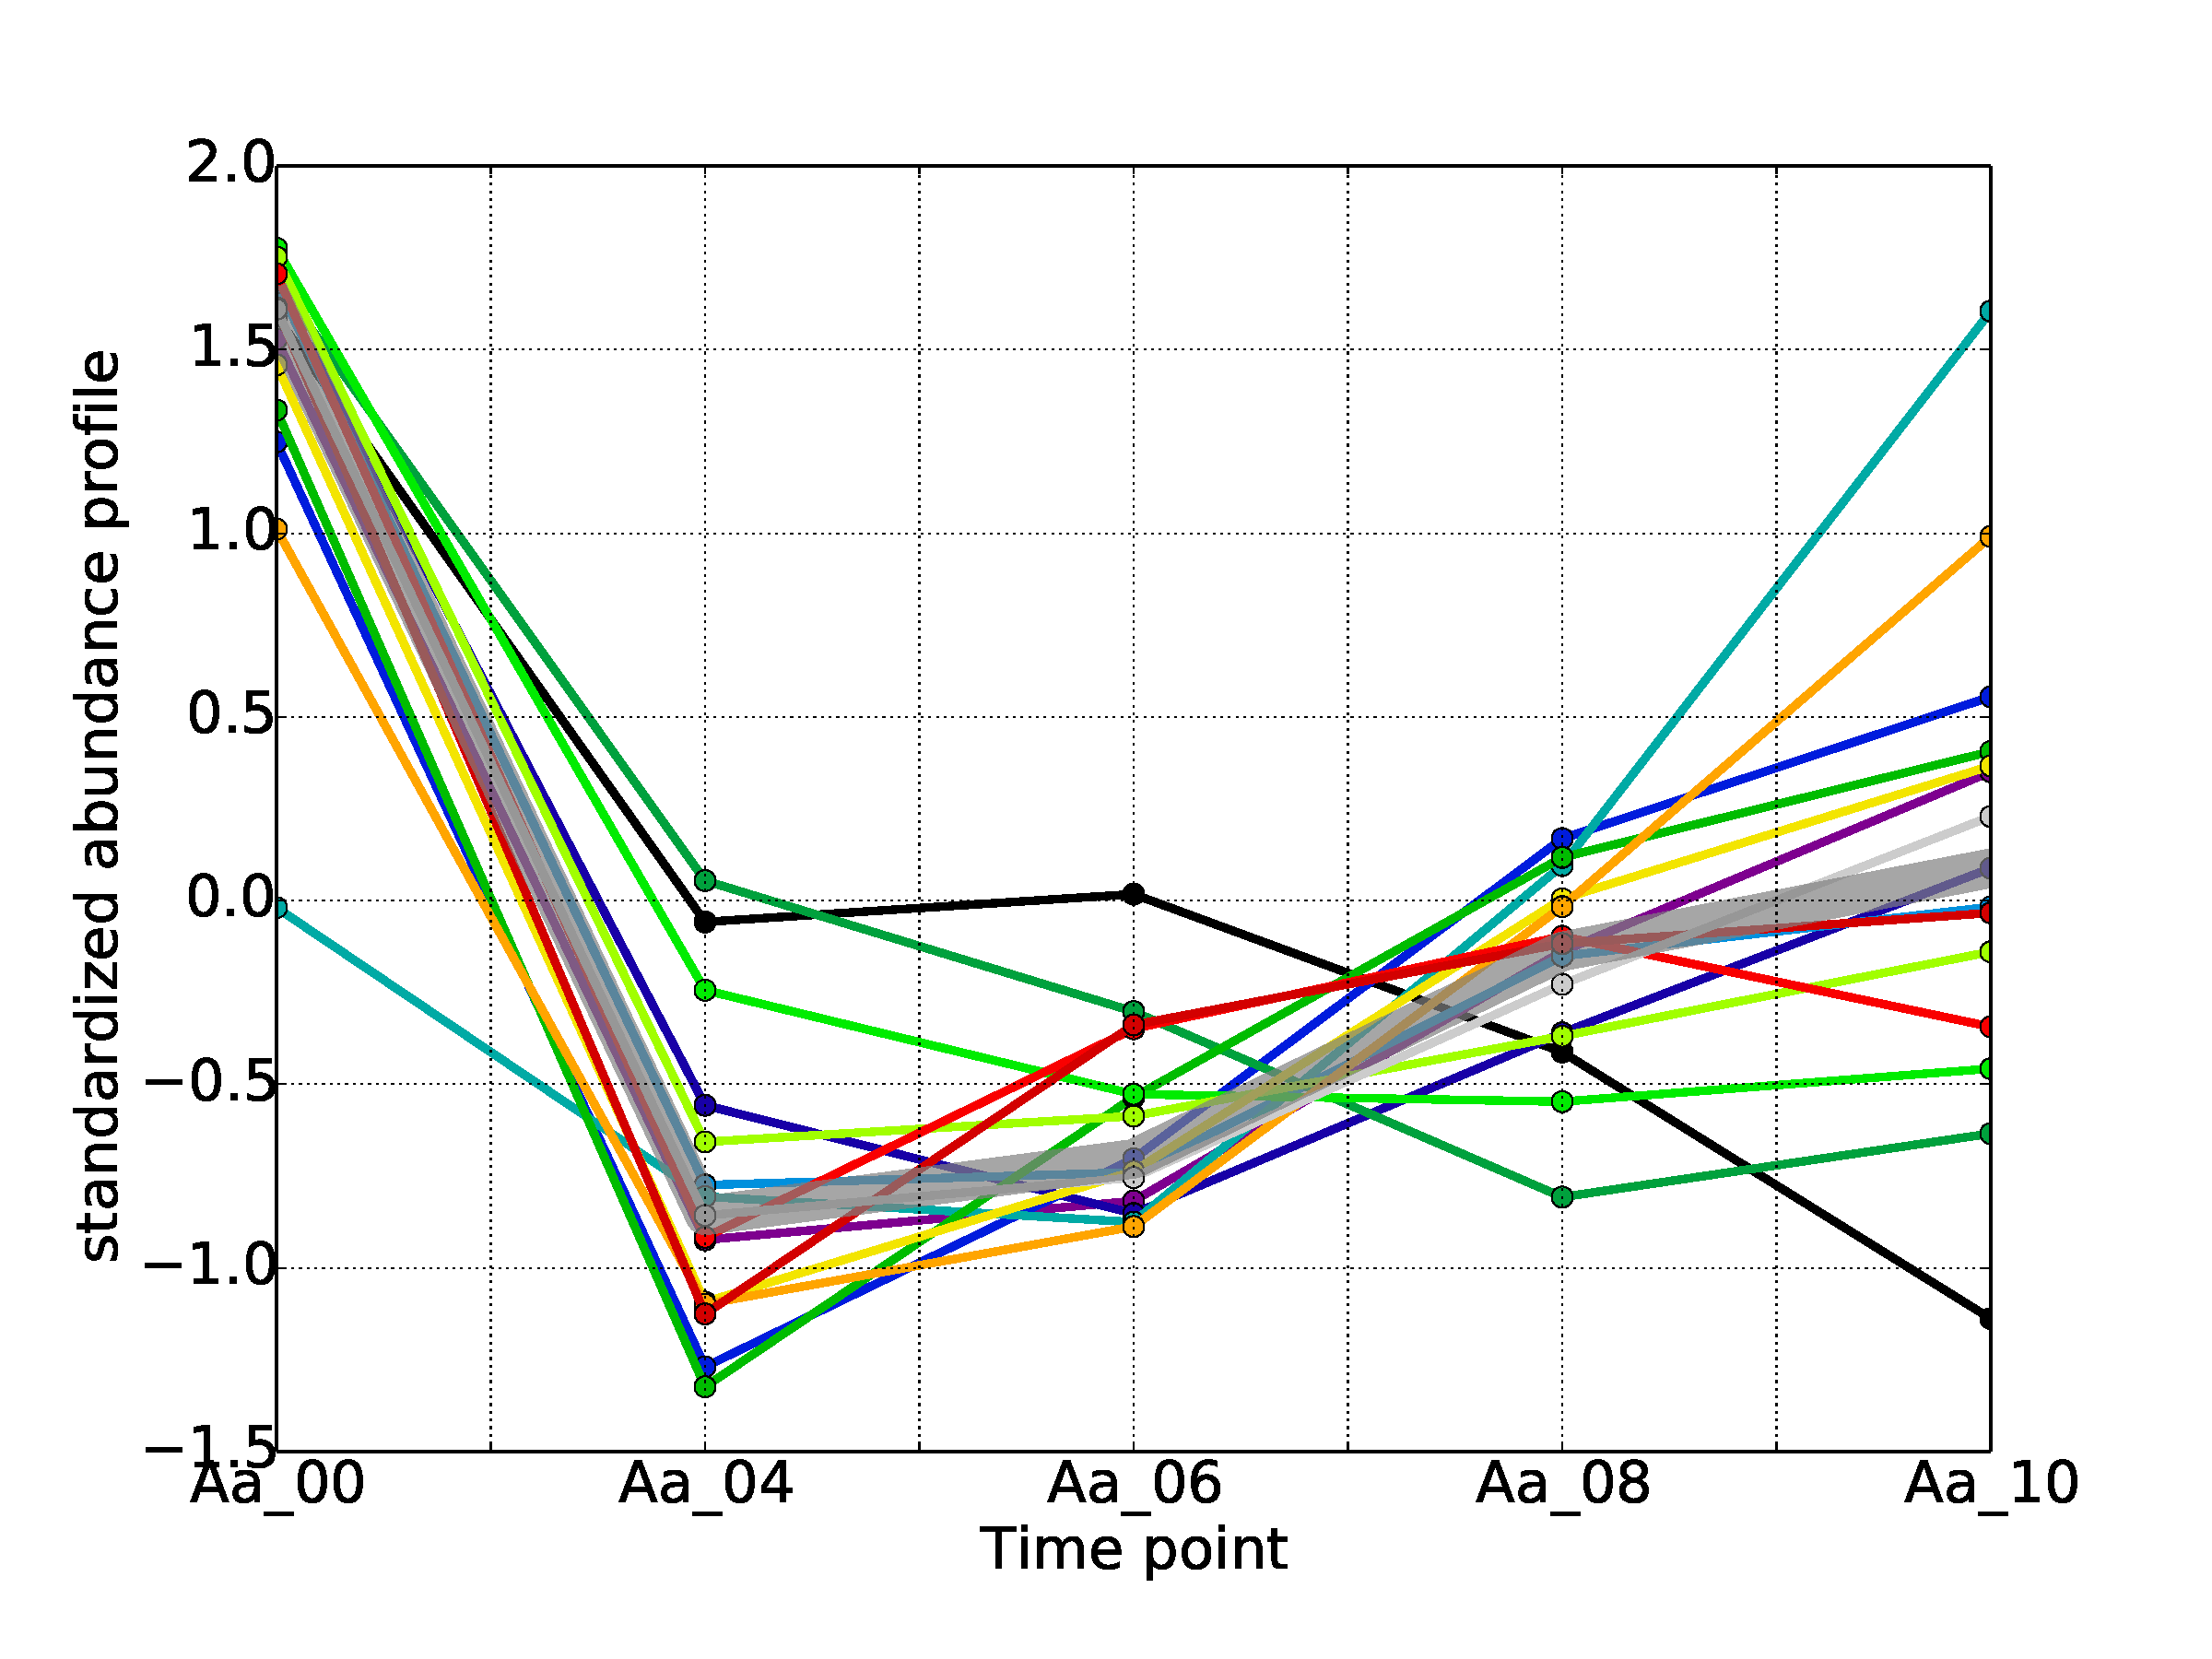
\includegraphics[width=.5\linewidth]{figures/figs/ecr_and_insects_ptci_20130918_orthodb7/downAt4_gene_profiles_from_cummerbund/Aa_downAt4_cls16_Ag_target_FPKMs_vb_orthos.pdf}}
%
\subcaptionbox{\label{fig:cluster16-Ag}}
{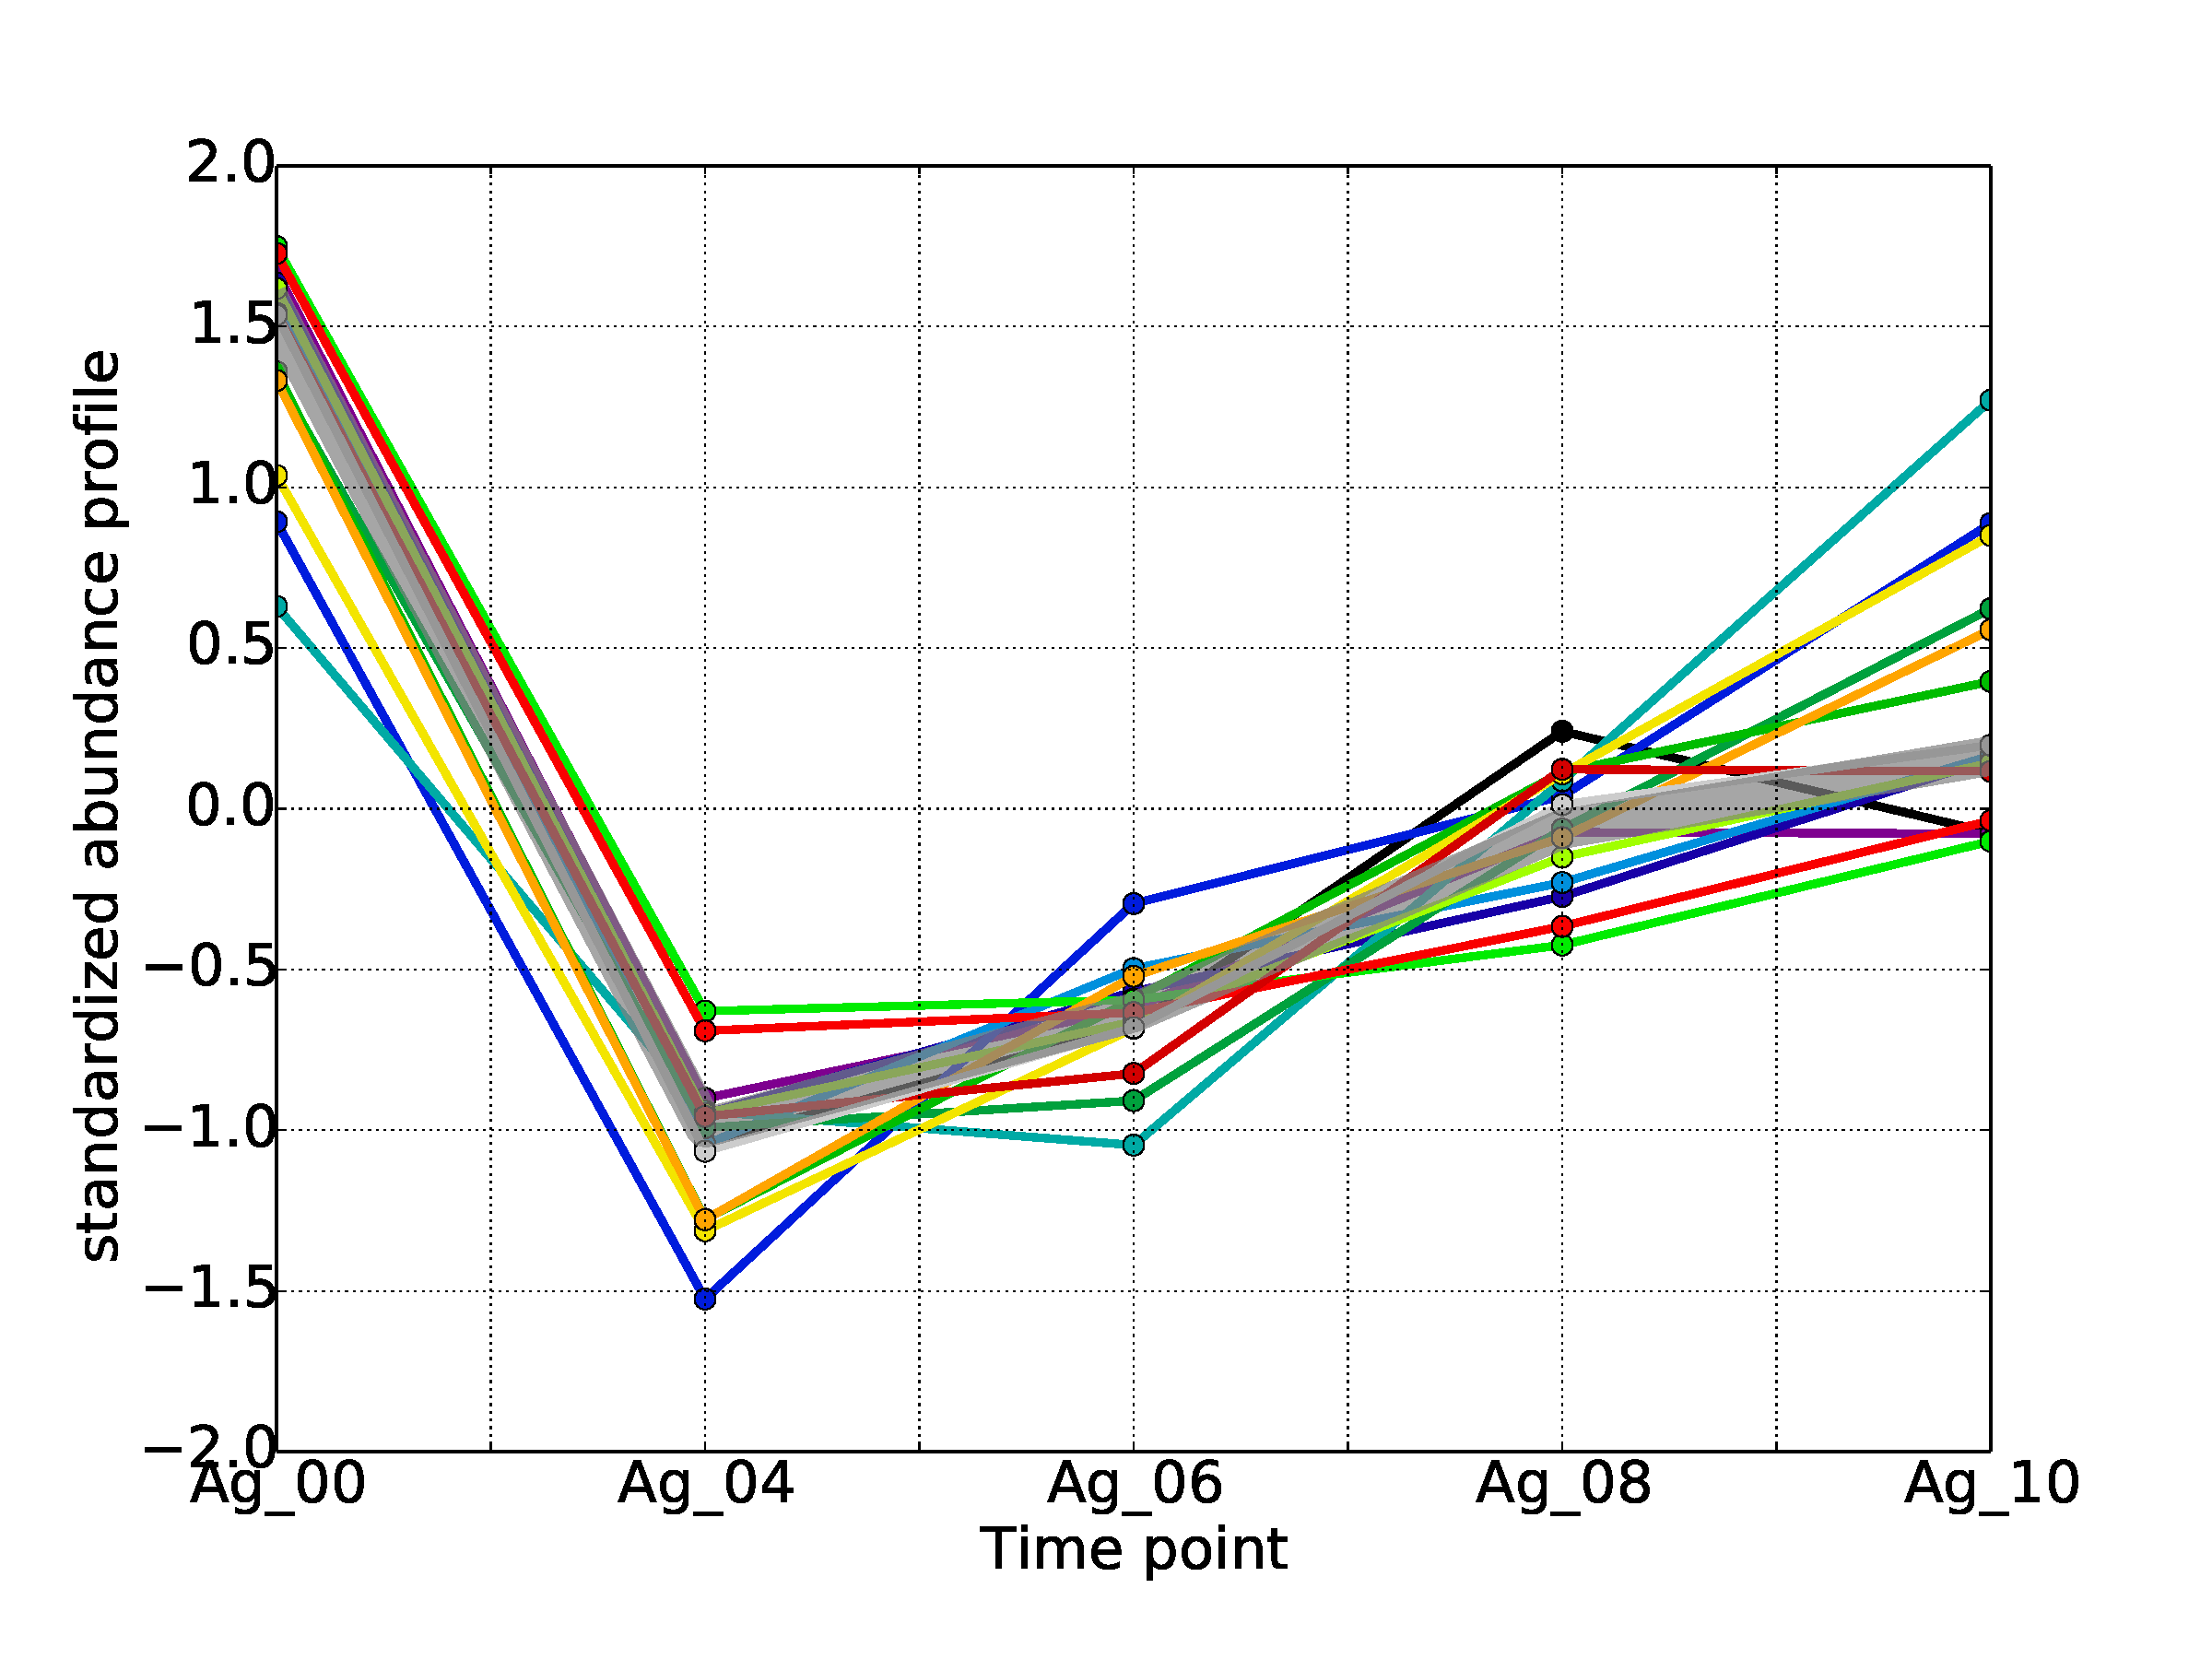
\includegraphics[width=.5\linewidth]{figures/figs/ecr_and_insects_ptci_20130918_orthodb7/downAt4_gene_profiles_from_cummerbund/Ag_downAt4_cls16_Ag_target_FPKMs_vb_orthos.pdf}}
%
\subcaptionbox{\label{fig:cluster16-Cq}}
{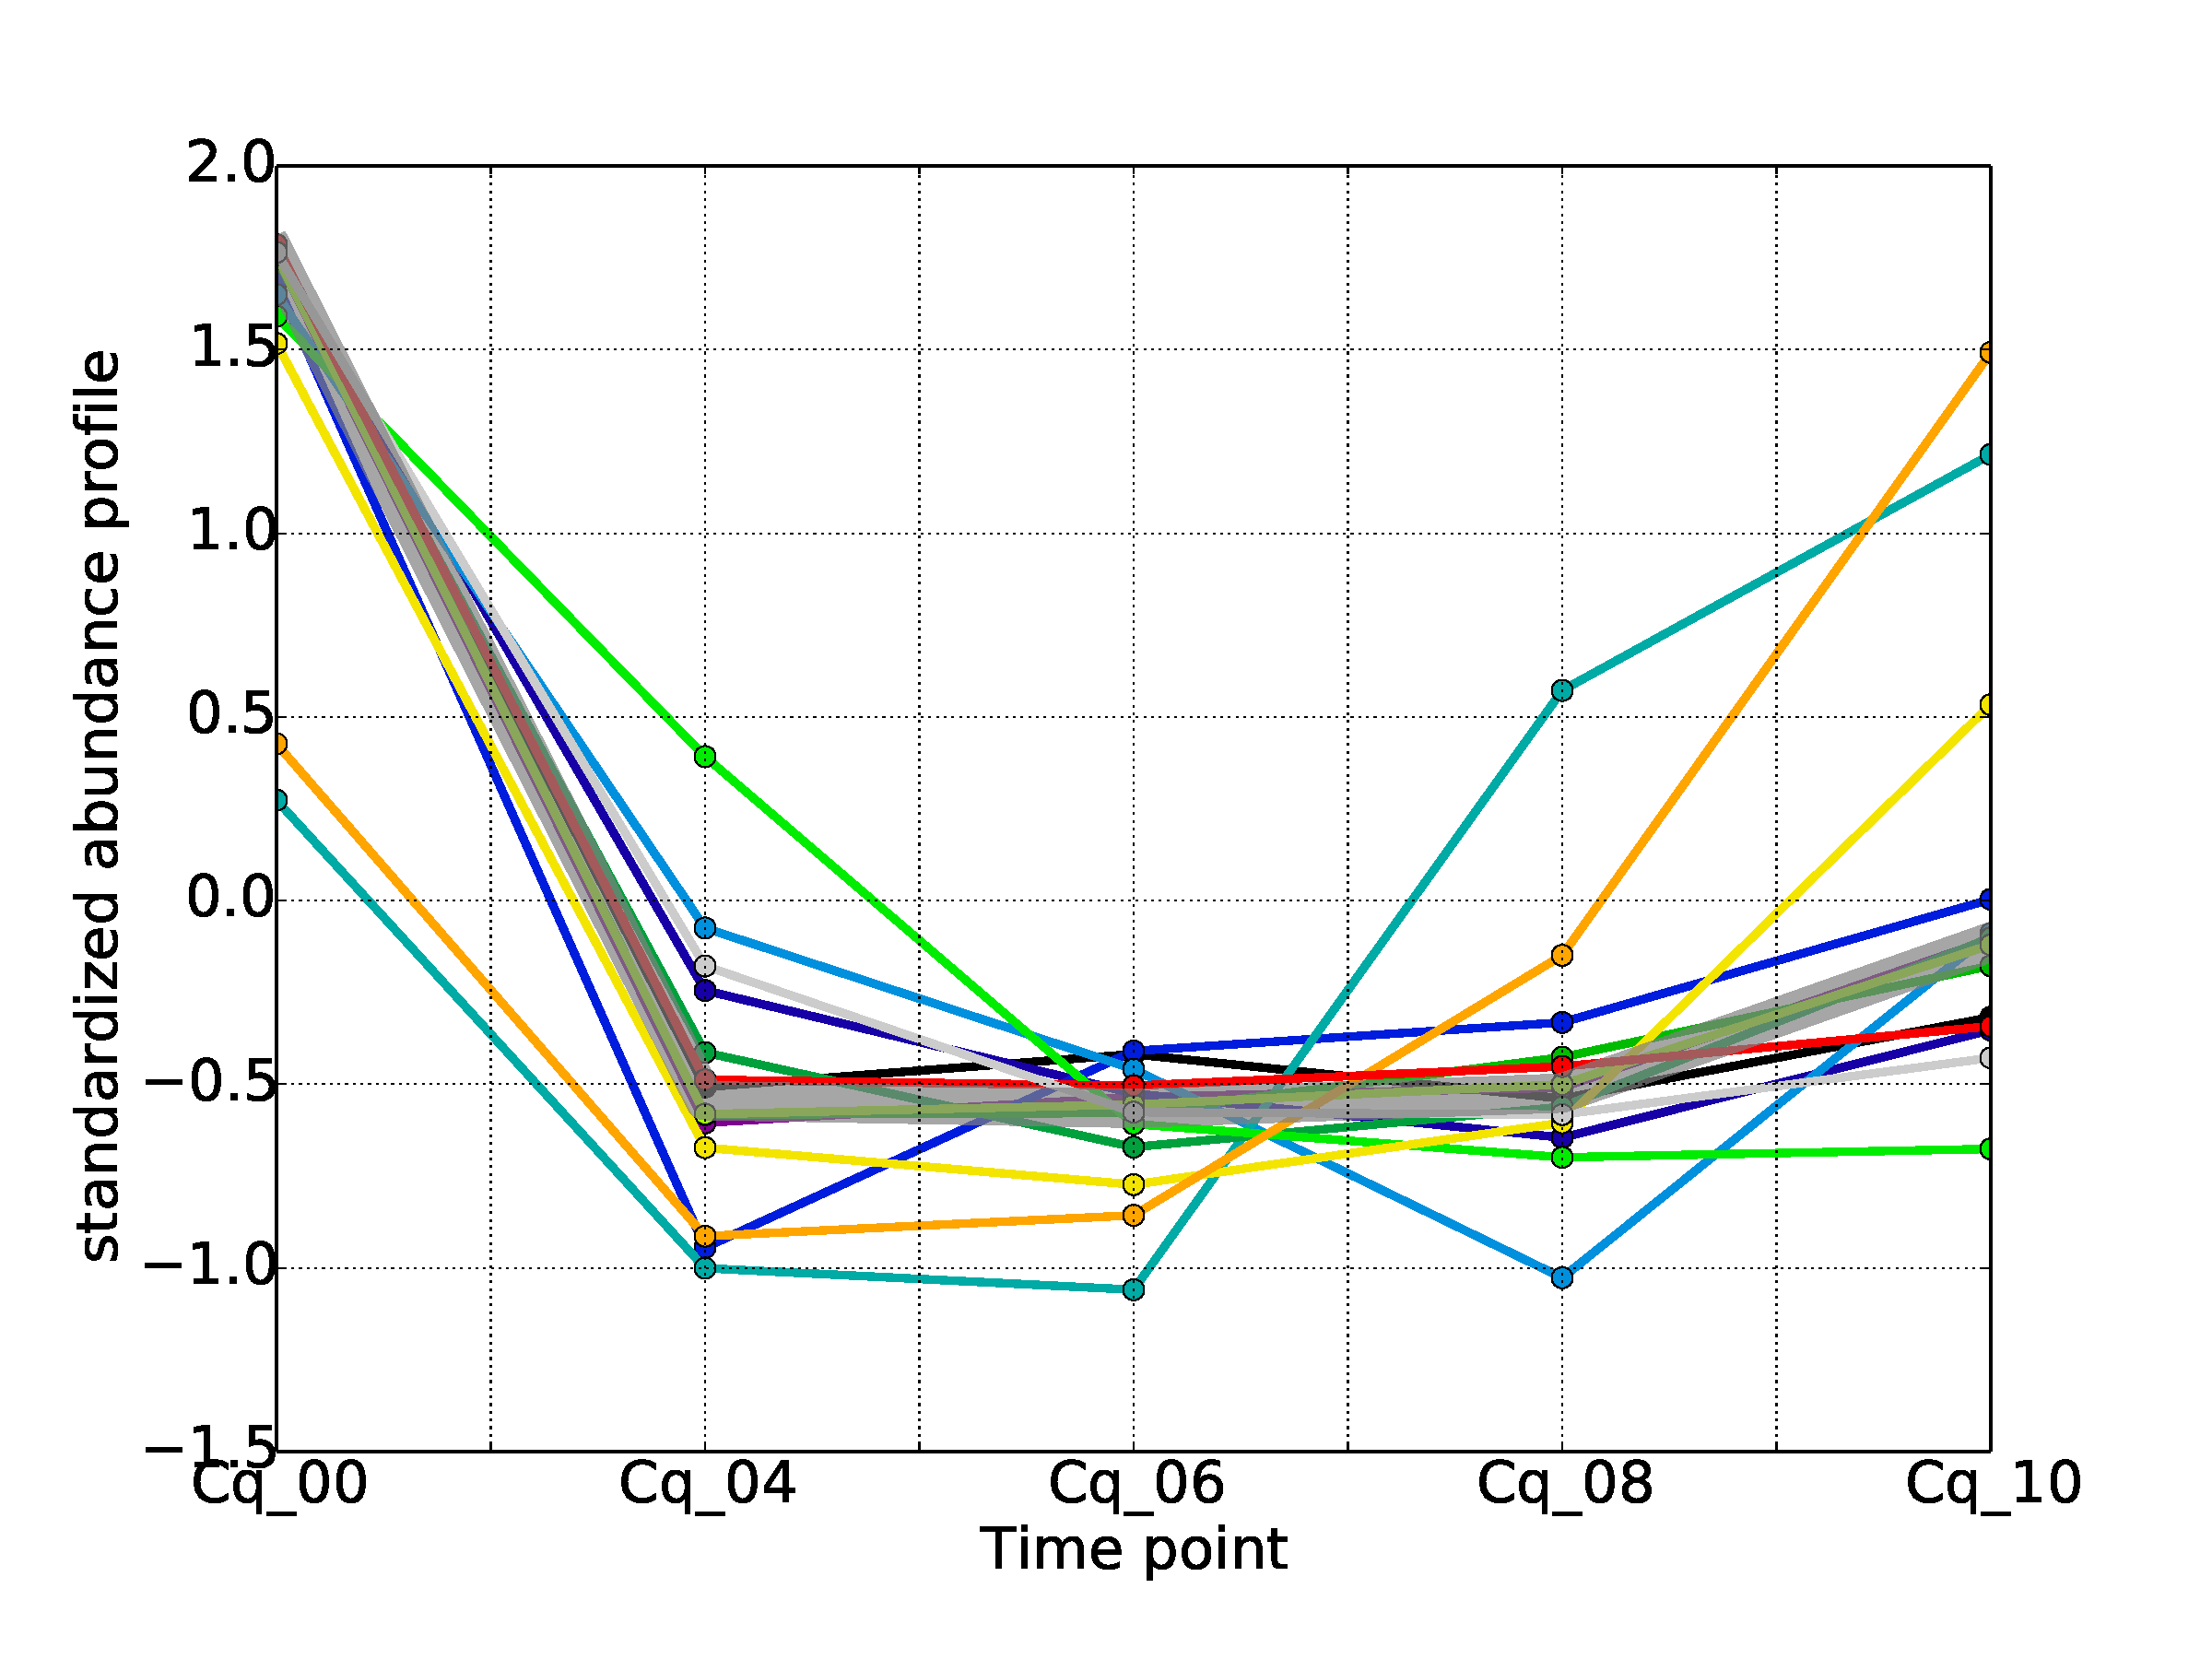
\includegraphics[width=.5\linewidth]{figures/figs/ecr_and_insects_ptci_20130918_orthodb7/downAt4_gene_profiles_from_cummerbund/Cq_downAt4_cls16_Ag_target_FPKMs_vb_orthos.pdf}}
% 
\caption[Orthologs of cluster 16]{\sf \textbf{Orthologs of cluster 16 (down at 4h):}\\
The same color scheme is used for each species which means that orthologs are given the same color in all three panels.
The thick, transparent gray line represents the median \gls{mAP} for the panel.
\textbf{(A)} \Aa.
\textbf{(B)} \Ag.
\textbf{(C)} \Cq.
}\label{fig:cluster16}
\end{figure}


\paragraph*{Functional annotations of cluster 16:}

% Downreulation of carbohydrate metabolism
% downregulation of autophagy/apoptotic process (yippee)/cellular arrest
% dwnreg of translation-repression
%   AAEL002550	 AGAP001639	 CPIJ002368 from OrthoDB

Cluster 16 contains genes with annotations that largely fit into the areas of carbohydrate digestion, cellular arrest, and repression of translation (Tables \ref{tab:cls16-process} and \ref{tab:cls16-process}).
%
Two ortholog-sets produced errors during the process that parsed the \gls{Argot2} results and others returned no process or function domain terms.
%
In these cases, OrthoDB was used to examine annotation terms assigned to these ortholog-sets using the OrthoDB ``metazoa'' database, and are noted as OrthoDB results.

% Booktabs require to add \usepackage{booktabs} to your document preamble
\begin{table}[h]
\begin{center} \sf
\begin{tabular}{p{.7\textwidth}r}
\toprule
\textbf{Name}                                 & \textbf{Total Score (mean)} \\ \midrule
one-carbon metabolic process                  & 8498.68                     \\
carbohydrate metabolic process                & 4077.43                     \\
translation                                   & 3505.77                     \\
regulation of Rho protein signal transduction & 1336.90                     \\
homophilic cell adhesion                      & 1316.75                     \\
cell adhesion                                 & 851.76                      \\
autophagy                                     & 686.01                      \\
apoptotic process                             & 670.22                      \\
regulation of myelination                     & 618.20                      \\
protein phosphorylation                       & 542.93                      \\
phosphorylation                               & 395.02                      \\
metabolic process                             & 286.58                      \\
protein transport                             & 262.15                      \\
protein ubiquitination                        & 242.49                      \\
intracellular signal transduction             & 212.22                      \\ \bottomrule
\end{tabular}
\end{center}

\caption[Cluster 16 top process GO terms]{\sf \textbf{Cluster 16 top process GO terms}}
\label{tab:cls16-process}
\end{table}
% Booktabs require to add \usepackage{booktabs} to your document preamble
\begin{table}[h]
\begin{center} \sf
\begin{tabular}{p{.7\textwidth}r}
\toprule
\textbf{Name}                                                    & \textbf{Total Score (mean)} \\ \midrule
carbonate dehydratase activity                                   & 4264.07                     \\
cysteine-type peptidase activity                                 & 2253.39                     \\
carbon-nitrogen ligase activity, with glutamine as amido-N-donor & 1652.90                     \\
Rho guanyl-nucleotide exchange factor activity                   & 1446.25                     \\
zinc ion binding                                                 & 1412.73                     \\
guanyl-nucleotide exchange factor activity                       & 1208.72                     \\
nucleic acid binding                                             & 810.14                      \\
peptidase activity                                               & 715.27                      \\
beta-tubulin binding                                             & 707.48                      \\
hydrolase activity, acting on glycosyl bonds                     & 652.43                      \\
glutaminyl-tRNA synthase (glutamine-hydrolyzing) activity        & 550.56                      \\
protein binding                                                  & 433.44                      \\
protein serine/threonine kinase activity                         & 413.31                      \\
metal ion binding                                                & 408.70                      \\
microtubule binding                                              & 403.62                      \\
ATP binding                                                      & 395.77                      \\
transferase activity                                             & 387.71                      \\
maltose alpha-glucosidase activity                               & 378.58                      \\
hydrolase activity                                               & 366.71                      \\
catalytic activity                                               & 331.87                      \\
ligase activity                                                  & 310.07                      \\
alpha-glucosidase activity                                       & 285.38                      \\
nucleotide binding                                               & 239.99                      \\
lyase activity                                                   & 212.94                      \\
oxidoreductase activity                                          & 206.49                      \\
protein kinase activity                                          & 200.95                      \\ \bottomrule                   
\end{tabular}
\end{center}

\caption[Cluster 16 top function GO terms]{\sf \textbf{Cluster 16 top function GO terms}}
\label{tab:cls16-function}
\end{table}

Terms relating to carbohydrate digestion are carbohydrate metabolic process (4077.43), maltose alpha-glucosidase activity (378.58), hydrolase activity (366.71), and alpha-glucosidase activity (285.38).

Cellular arrest terms assigned by \gls{Argot2} include autophagy (686.01) and apoptotic process (670.22).

%
Additionally, OrthoDB results identified one ortholog-set (AAEL002833, AGAP011828, CPIJ006471) as orthologs to \Dm\ Cathepsin L which FlyBase annotates with biological process terms including proteolysis, autophagic cell death, protein catabolic process, and salivary gland cell autophagic cell death.
%

Terms pertaining to the repression of translation were obtained from the ortholog-set including AAEL002550, AGAP001639, and CPIJ002368 via OrthoDB.
%
Process results include 32 genes with negative regulation of translational initiation (GO:0045947), and function results contain 17 genes with translation repressor activity, nucleic acid binding (GO:0000900); 15 genes with translation repressor activity (GO:0030371); and 2 genes with  poly(A) RNA binding (GO:0008143:).



\subsubsection{Cluster 22 (up at 4h)}

\paragraph*{General description:}

Cluster 22 is characterized by genes that have a median \gls{NBF} \gls{FPKM} of between 0 and 0.5 standard deviations \textit{below} the overall mean \gls{FPKM} and a 4h \gls{PBM} median \gls{FPKM} value of approximately 1.5 standard deviations \textit{above} the overall mean \gls{FPKM}. The median \gls{FPKM} values for the remaining time points then gradually approach approximately 1 standard deviations \textit{below} the overall mean \gls{FPKM} by the end of the time course (Figures \ref{fig:23-clusters} and \ref{fig:cluster22}).
%
This \gls{mAP} illustrates a rapid and substantial but temporary increase in mRNA abundance following bloodfeeding.
%
\begin{figure}[p]
% 
\subcaptionbox{\label{fig:cluster22-Aa}}
{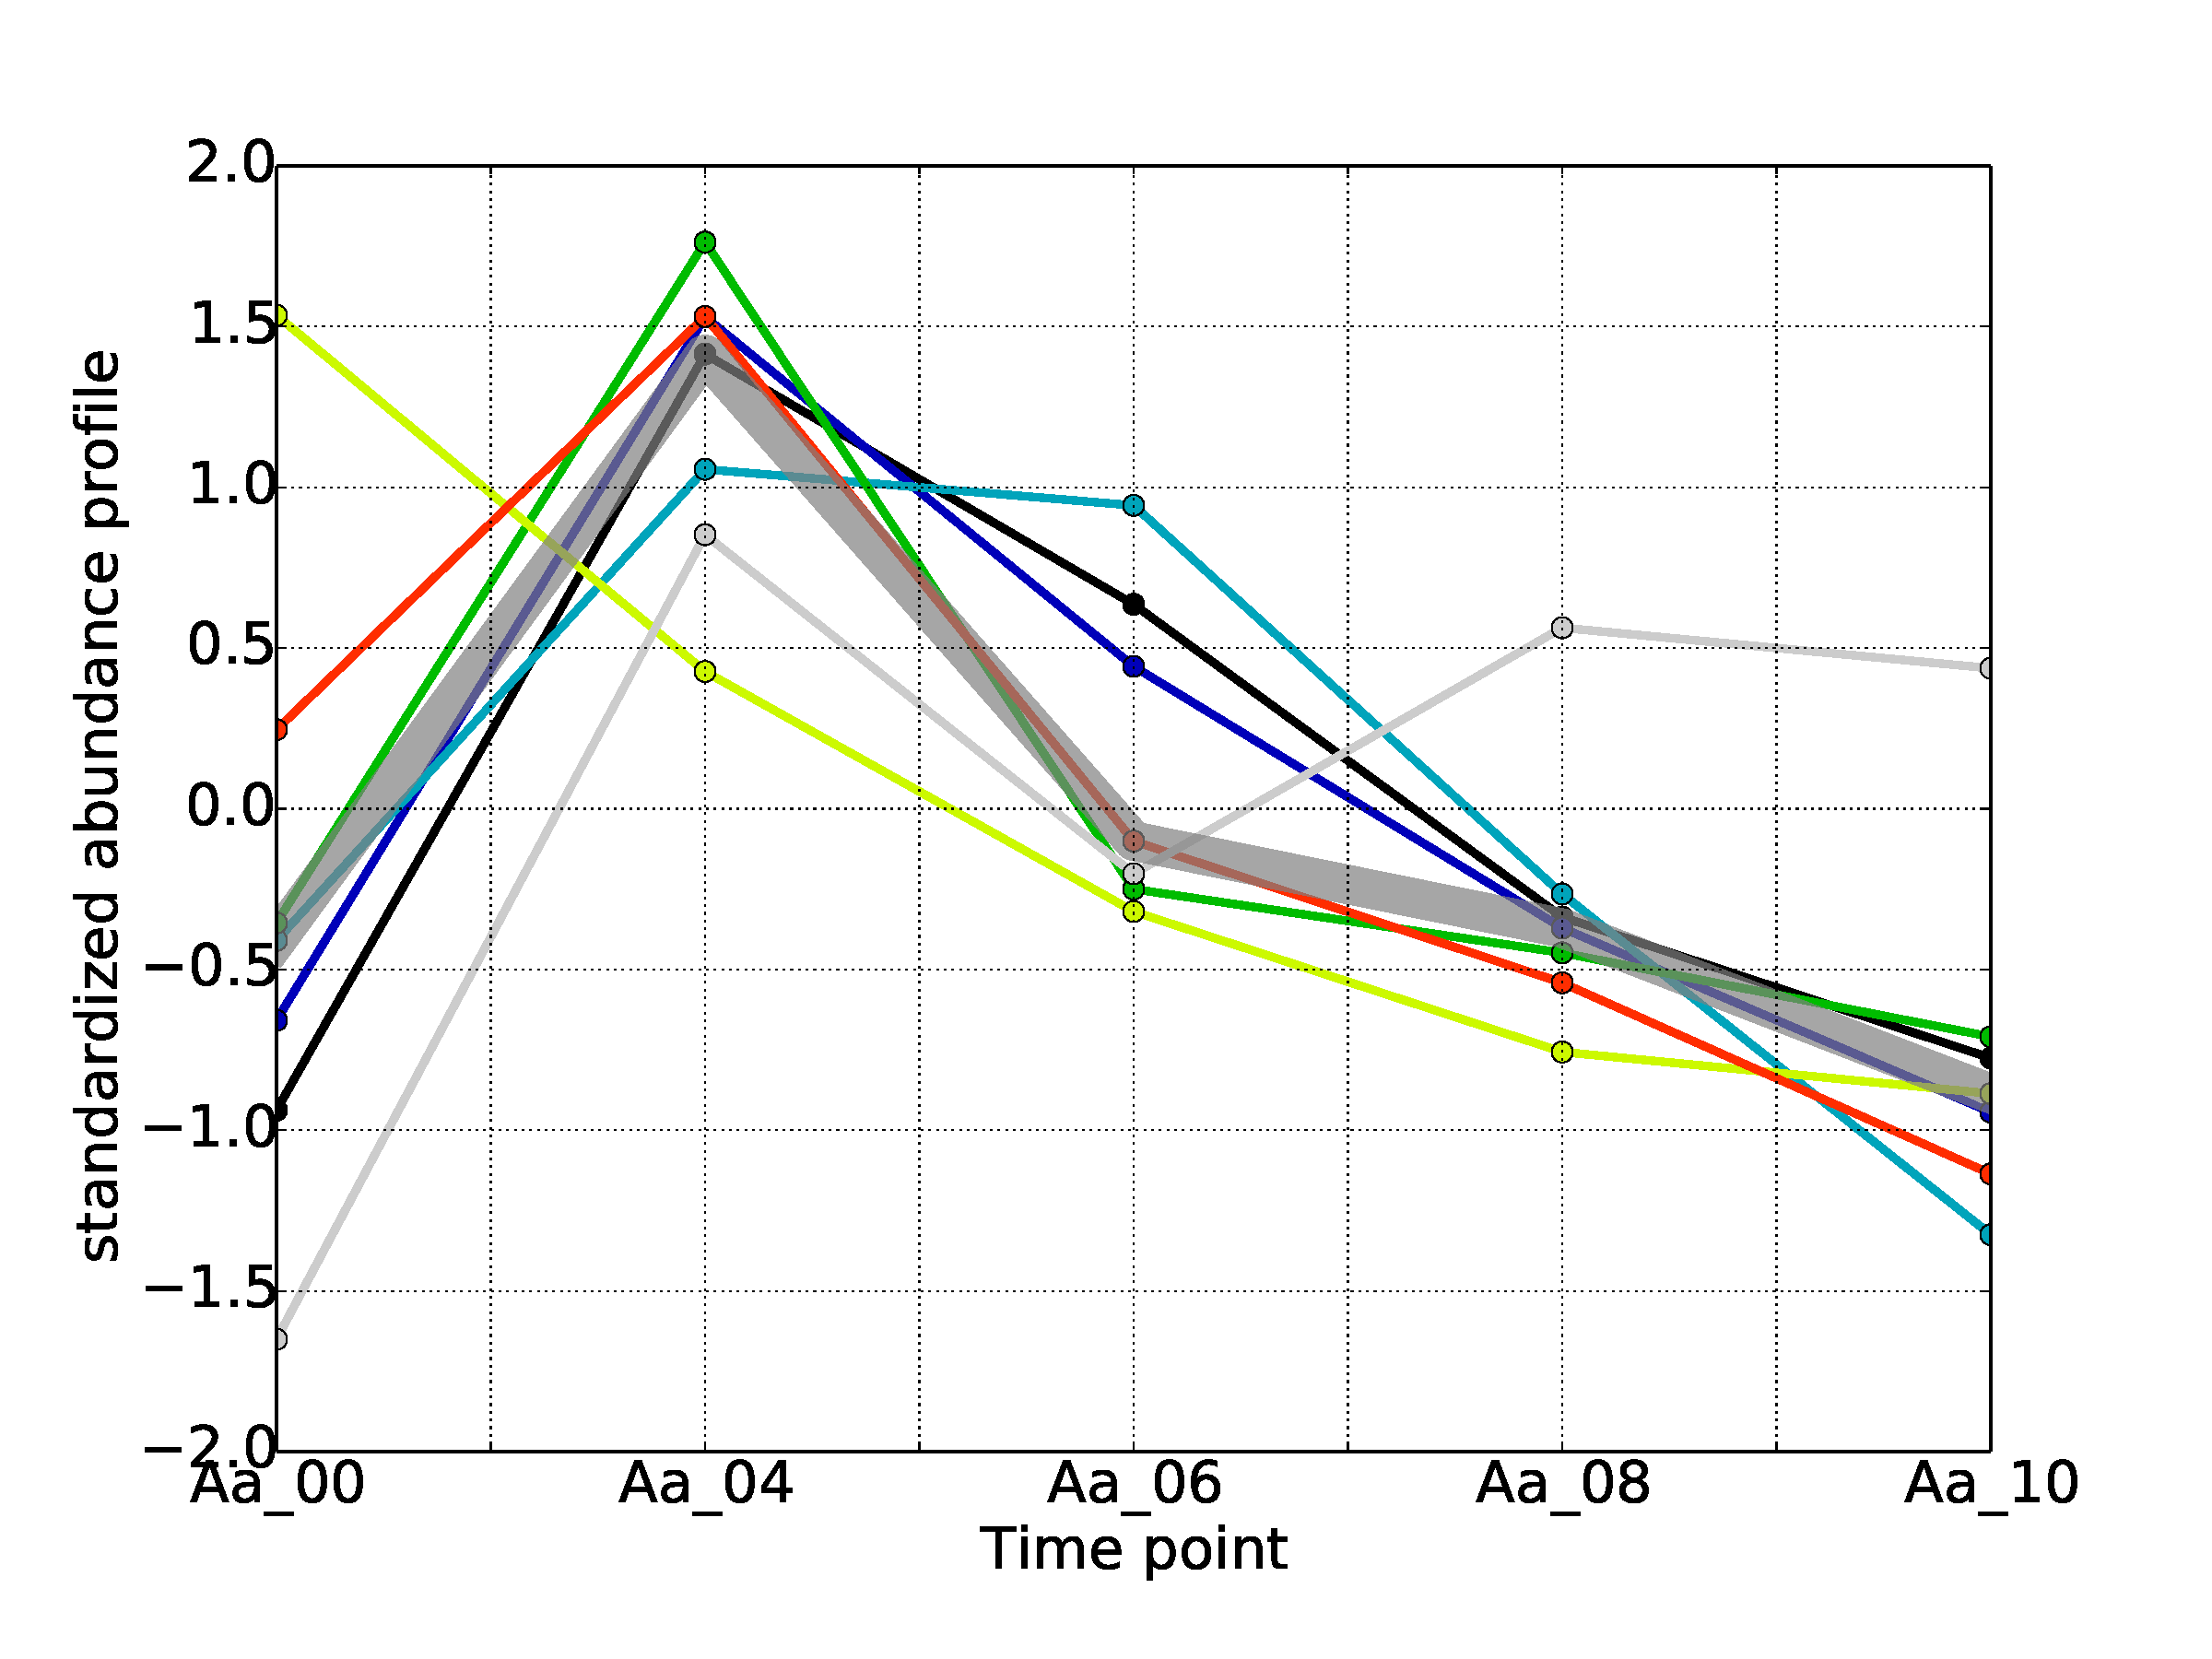
\includegraphics[width=.5\linewidth]{figures/figs/ecr_and_insects_ptci_20130918_orthodb7/upAt4_gene_profiles_from_cummerbund/Aa_upAt4_cls22_Ag_target_FPKMs_vb_orthos.pdf}}
%
\subcaptionbox{\label{fig:cluster22-Ag}}
{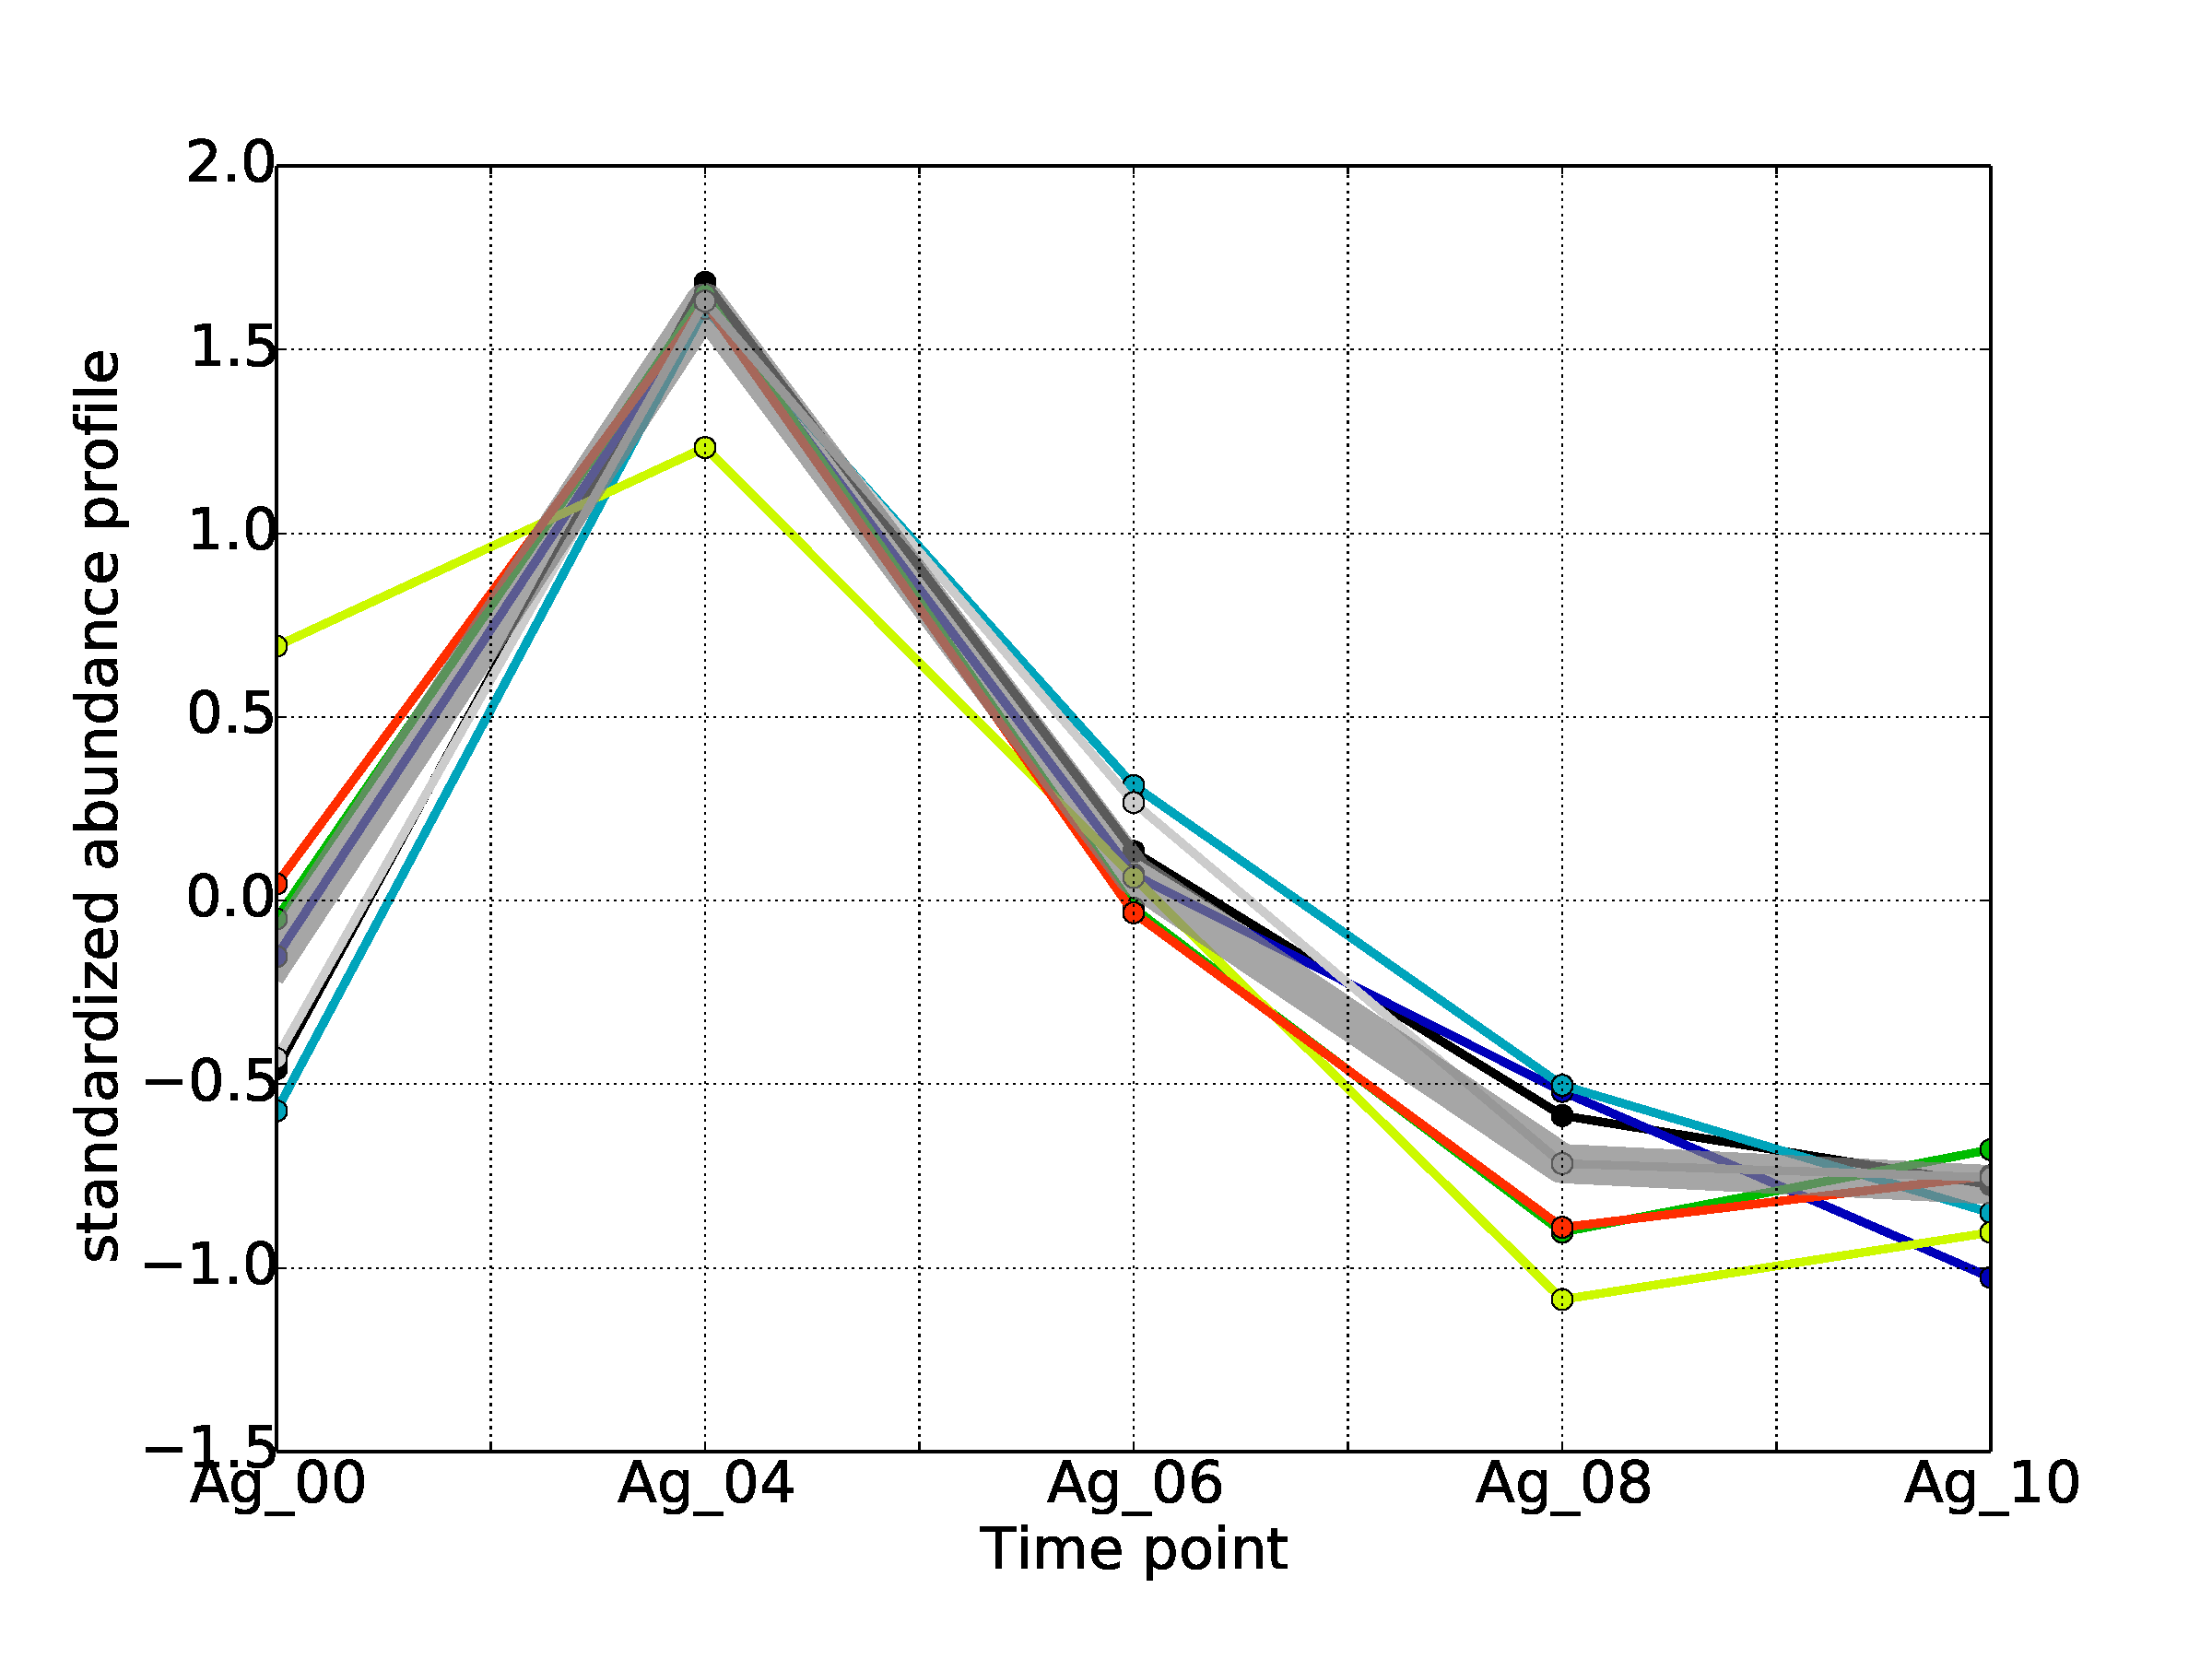
\includegraphics[width=.5\linewidth]{figures/figs/ecr_and_insects_ptci_20130918_orthodb7/upAt4_gene_profiles_from_cummerbund/Ag_upAt4_cls22_Ag_target_FPKMs_vb_orthos.pdf}}
%
\subcaptionbox{\label{fig:cluster22-Cq}}
{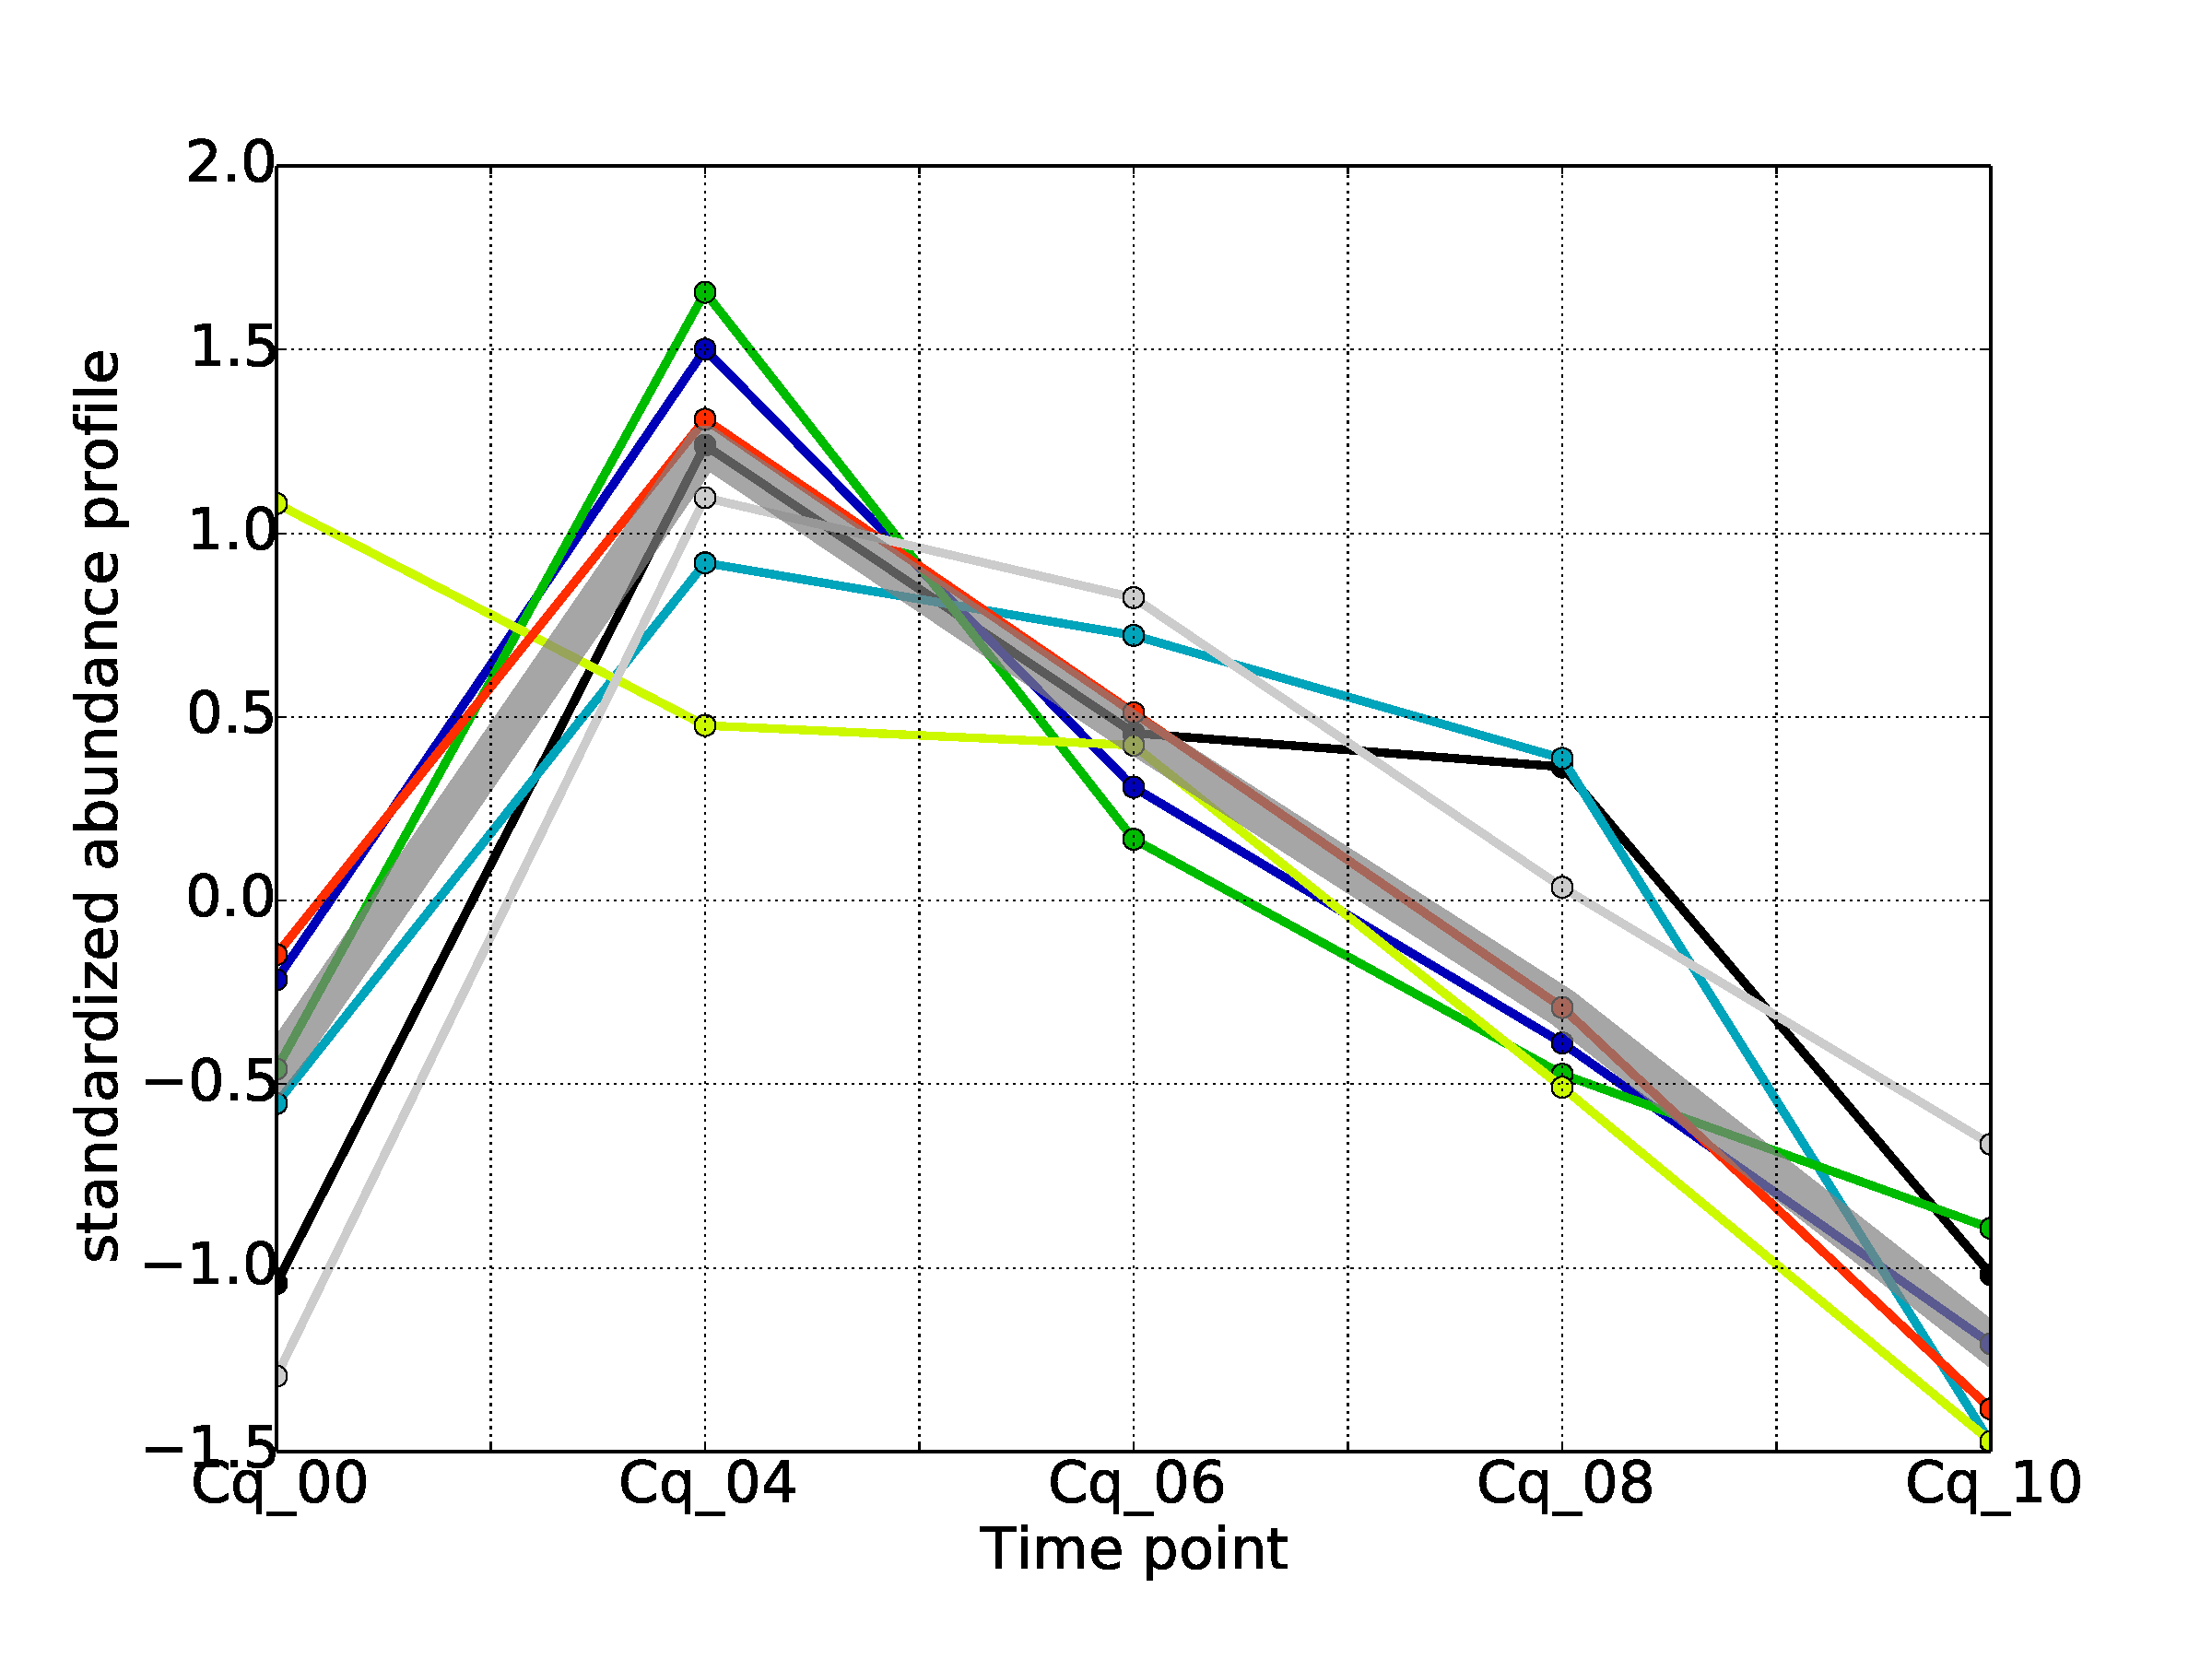
\includegraphics[width=.5\linewidth]{figures/figs/ecr_and_insects_ptci_20130918_orthodb7/upAt4_gene_profiles_from_cummerbund/Cq_upAt4_cls22_Ag_target_FPKMs_vb_orthos.pdf}}
% 
\caption[Orthologs of cluster 22]{\sf \textbf{Orthologs of cluster 22 (up at 4h):}\\
The same color scheme is used for each species which means that orthologs are given the same color in all three panels.
The thick, transparent gray line represents the median \gls{mAP} for the panel.
\textbf{(A)} \Aa.
\textbf{(B)} \Ag.
\textbf{(C)} \Cq.
}\label{fig:cluster22}
\end{figure}


\paragraph*{Functional annotations of cluster 22:}

% protein folding / translation
% membrane transport
% chromatin reoganization / link to 20E signaling pathway

% ## not found in func annotation mean tables ## AAEL011240	 AGAP006534	 CPIJ002990  --> ortholog to Dmel putzig (ptz)  annotated as described with: positive regulation of Notch signaling pathway; negative regulation of JAK-STAT cascade; chromosome organization; ecdysone receptor-mediated signaling pathway; cell cycle; neurogenesis; chromatin organization.


% transcription factors
%	AAEL011240, AGAP006534, CPIJ002990 {ortholog to Dmel putzig (ptz)}
%	AAEL002795, AGAP003943, CPIJ004011 {Rfx transcription factor}


Cluster 2 has the fewest members of ortholog-sets of the four clusters described here (7 members per species) (Figure \ref{fig:23-clusters}).
%
The putative functions in this cluster can be associated with protein translation and protein folding; transcription regulation; and chromatin reorganization (Tables \ref{tab:cls22-process} and \ref{tab:cls22-function}).
%
Terms associated with protein translation and folding include translation initiation factor activity (20221.31), unfolded protein binding (7160.14), lysyl-tRNA aminoacylation (5305.2), regulation of translational initiation (5198.1), protein folding (5145.4), translation (3885.2), tRNA aminoacylation for protein translation (3277.1), translational initiation (3268.5), cellular protein metabolic process (2591.6), formation of translation preinitiation complex (1607.7), and tRNA processing (223.64).

% Booktabs require to add \usepackage{booktabs} to your document preamble
\begin{table}[hp]
\begin{center} \sf
\begin{tabular}{p{.7\textwidth}r}
\toprule
\textbf{Name}                                  & \textbf{Total Score (mean)} \\ \midrule
lysyl-tRNA aminoacylation                      & 5305.29                     \\
regulation of translational initiation         & 5198.13                     \\
protein folding                                & 5145.48                     \\
translation                                    & 3885.25                     \\
tRNA aminoacylation for protein translation    & 3277.15                     \\
translational initiation                       & 3268.53                     \\
cellular protein metabolic process             & 2591.65                     \\
regulation of transcription, DNA-dependent     & 2500.50                     \\
transmembrane transport                        & 2120.54                     \\
formation of translation preinitiation complex & 1607.78                     \\
transcription, DNA-dependent                   & 1314.06                     \\
signal transduction                            & 853.12                      \\
regulation of insulin secretion                & 709.97                      \\
negative regulation of BMP signaling pathway   & 526.20                      \\
regulation of cell cycle                       & 470.82                      \\
melanocyte differentiation                     & 316.77                      \\
endocrine pancreas development                 & 296.05                      \\
transport                                      & 288.59                      \\
developmental pigmentation                     & 287.51                      \\
pigmentation                                   & 273.58                      \\
tRNA processing                                & 223.64                      \\
multicellular organismal development           & 203.63                      \\ \bottomrule
\end{tabular}
\end{center}

\caption[Cluster 22 top process GO terms]{\sf \textbf{Cluster 22 top process GO terms}}
\label{tab:cls22-process}
\end{table}
% Booktabs require to add \usepackage{booktabs} to your document preamble
\begin{table}[hp]
\begin{center} \sf
\begin{tabular}{p{.7\textwidth}r}
\toprule
\textbf{Name}                               & \textbf{Total Score (mean)} \\ \midrule
translation initiation factor activity      & 20221.31                    \\
unfolded protein binding                    & 7160.14                     \\
DNA binding                                 & 4535.66                     \\
arsenite transmembrane transporter activity & 1600.53                     \\
lysine-tRNA ligase activity                 & 1557.61                     \\
cytoskeletal adaptor activity               & 1456.65                     \\
ATP binding                                 & 1146.99                     \\
aminoacyl-tRNA ligase activity              & 682.47                      \\
nucleotide binding                          & 669.32                      \\
ligase activity                             & 526.89                      \\
transporter activity                        & 400.96                      \\
zinc ion binding                            & 257.13                      \\ \bottomrule                     
\end{tabular}
\end{center}

\caption[Cluster 22 (up at 4h) mean function GO terms]{\sf \textbf{Cluster 22 (up at 4h) mean function GO terms}}
\label{tab:cls22-function}
\end{table}

Two ortholog-sets are annotated as transcription factors (AAEL011240, AGAP006534, CPIJ002990: orthologs to \Dm\ putzig; and AAEL002795, AGAP003943, CPIJ004011: Rfx transcription factors).
%
FlyBase has annotated putzig with the following terms in \Dm, positive regulation of Notch signaling pathway; negative regulation of JAK-STAT cascade; chromosome organization; ecdysone receptor-mediated signaling pathway; cell cycle; neurogenesis; and chromatin organization \cite{Marygold2013}.
%
The Rfx transcription factors were assigned regulation of insulin secretion (709.97) and endocrine pancreas development (296.05) by \gls{Argot2}.
%
OrthoDB corroborates these annotations, but only when the database includes metazoa.

Membrane transport and signaling terms are also present.
%
They are arsenite transmembrane transporter activity (1600.53), transporter activity (400.96), transmembrane transport (2120.5), signal transduction (853.12), negative regulation of BMP signaling pathway (526.20), regulation of cell cycle (470.82), and transport (288.59).








\section{Discussion} \label{chap:4-sec:discussion}


% Cluster 4
% upregulation of translation/TOR
%	peptide quality control 
% active secretory pathways in both directions
% Metabolic activities

% Heme management
% midgut repair

%%%%%%%%%%%%%%%%%%%%%%%%%%%%%%

% Cluster 6
% downregulation of transcription factors
% translation elongation
% signaling
% Heme management

% transcription factors
%	X AGAP002238:AAEL010222CPIJ008350 {GATA-type}
%	x AAEL009171:CPIJ001396:AGAP003726 {ortholog to Dmel bZIP family. CREBRF subfamily}
%	x CPIJ004057:AAEL009114:AGAP004050 {Doublesex}
%	x CPIJ014945:AAEL002062:AGAP005661 {Ftz-f1}
%	x AAEL001361:AGAP006990:CPIJ002241 {Bap 170 }
%	x CPIJ005607:AAEL005452:AGAP010201 {ortholog to Dmel crp}

%%%%%%%%%%%%%%%%%%%%%%%%%%%%%%

% Cluster 16

% Downreulation of carbohydrate metabolism
% downregulation of autophagy/apoptotic process (yippee)/cellular arrest
% dwnreg of translation-repression
%   AAEL002550	 AGAP001639	 CPIJ002368 from OrthoDB

%%%%%%%%%%%%%%%%%%%%%%%%%%%%%%

% Cluster 22

% protein folding / translation
% membrane transport
% chromatin reoganization / link to 20E signaling pathway

% ## not found in func annotation mean tables ## AAEL011240	 AGAP006534	 CPIJ002990  --> ortholog to Dmel putzig (ptz)  annotated as described with: positive regulation of Notch signaling pathway; negative regulation of JAK-STAT cascade; chromosome organization; ecdysone receptor-mediated signaling pathway; cell cycle; neurogenesis; chromatin organization.


% transcription factors
%	AAEL011240, AGAP006534, CPIJ002990 {ortholog to Dmel putzig (ptz)}
%	AAEL002795, AGAP003943, CPIJ004011 {Rfx transcription factor}

Clusters 4, 6, 16, and 22 do not constitute a comprehensive representation of midgut transcription profiles.
%
The clusters are only four of 23 from the partitioned set of \glspl{mAP} obtained by the \gls{gFunc} selection process.
%
Furthermore, the decision only to focus on genes that are members of 3-way 1:1 ortholog relationships restricted this study to roughly 30\% of the total genes annotated in each species from the beginning.
%
However, the aim of this study was not to produce a comprehensive overview but a concentrated view of a limited aspect of gene expression in the midgut based on \textit{a priori} objectives.
%
Clusters 4, 6, 16, and 22 represent the accomplishment of this aim.


The bloodmeal is an extremely important event in the reproduction of mosquitoes.
%
However, it also poses significant biochemical challenges that must be managed.
%
A few of these challenges include massive distention of the tissues of the midgut and abdomen by the volume of the blood; dangerous compounds and potential pathogens that are contained in the blood; and massive and systemic changes in genomic activity among various cell-types that are triggered by the bloodmeal.
%
Before the bloodmeal, the female begins the process of developing a clutch of eggs, but the process is halted and maintains a state of suspended development.
%
Upon ingestion of a sufficient volume of protein-rich blood, this suspension of development is lifted and various cell-types alter their signaling and genomic contexts as development of the clutch resumes.


The insulin and \gls{TOR} pathways are responsible for sensing the change in nutrient levels following a bloodmeal \cite{Roy2007}, \cite{Hietakangas2009}, [6\cite{Brandon2008}.
%
There are local and systemic aspects to nutrient sensing 5\cite{Hietakangas2009}.
%
Insulin, or insulin-like hormones, can transmit systemic signals through the hemolymph and contribute to \gls{TOR}-related, gene expression through interacting with \glspl{InR} on the cellular membrane.
%
This stimulates \gls{PI3K}, eventually resulting in de-repression of the TORC1 complex.
%
Local nutrient levels are sensed by monitoring energy (\gls{amp}-to-\gls{ATP} ratios) and amino acid levels.
%
TORC1 is repressed when \gls{amp}/\gls{ATP} is high and/or amino acid levels are low.
%
De-repression of TORC1 results in translation of specific pre-transcribed mRNAs and a general activation of translation.
%
Myc and FoxO transcription factors also mediate specific transcription events in response to TORC1.
%
Additionally, \gls{20E} titers gradually begin to rise immediately after bloodmeal ingestion, but the titers exhibit periodic peaks throughout the process (4h, 8h, and 24h \gls{PBM}) that coincide with specific events \cite{Hagedorn1975}.
%
Notably, a small but reproducible peak in 20E titer occurs four hours after blood feeding.
%
This coincides with many bloodmeal-related events such as a peak in posterior midgut aminopeptidase activity that has been noted in \As\ \cite{Billingsley1991}; an initiation of the increase of late trypsin in the midgut \cite{Barillasmury1991},\cite{Graf1988}; an increase of JH-esterase activity that causes a rapid decline of \gls{JH} \cite{Shapiro1986}, and an increase in transcript abundance of \gls{EcR} and associated transcription factors in the fat body \cite{Raikhel1999}.




\subsection{Integrative interpretation of the functional aspects of clusters 4, 6, 16, and 22} % \subsection{Bloodfeeding and the midgut}



\subsection{Interpretation of Argot2 results} % interpretation of Argot2 results (insulin/pancreas dev came from vertebrate matches and require a degree of interpretation)
% \lipsum[1]

\subsection{Heme management}
% \lipsum[1]



%%% Local Variables: ***
%%% mode: latex ***
%%% TeX-master: "thesis.tex" ***
%%% End: ***

\chapter{Contributions to Literature Not Otherwise Mentioned}
\todo[inline]{decide whether this gets included}
\section{Purpose}
xxxxxxxxxxxxxxxxxxxxxxxxxx
\begin{enumerate}
 \item xxx
\end{enumerate}


%%% Local Variables: ***
%%% mode: latex ***
%%% TeX-master: "thesis.tex" ***
%%% End: ***

\chapter{Conclusions}
\todo{replace CITEME tags in Introduction}

\todo{write all the figures}

\todo{MEGA: you need to write most of this chapter}
\section{Purpose}
xxxxxxxxxxxxxxxxxxxxxxxxxx
\begin{enumerate}
 \item xxx
\end{enumerate}

%%% Local Variables: ***
%%% mode: latex ***
%%% TeX-master: "thesis.tex" ***
%%% End: ***


% ... and so on

% These commands fix an odd problem in which the bibliography line
% of the Table of Contents shows the wrong page number.
\clearpage
\phantomsection

% "References should be formatted in style most common in discipline",
% abbrv is only a suggestion.
\bibliographystyle{plos_biology}
\bibliography{/home/gus/Dropbox/MendeleyBibTeX/thesis}
\citeindextrue

% The Thesis Manual says not to include appendix figures and tables in
% the List of Figures and Tables, respectively, so these commands from
% the caption package turn it off from this point onwards. If needed,
% it can be re-enabled later (using list=yes argument).
\captionsetup[figure]{list=no}
\captionsetup[table]{list=no}

% If you have an appendix, it should come after the references.
% The original template (from Trevor) had a custom \appendix command,
% but I found it to break figure/table counters. I'm not sure how
% reliable my fix is, so I ended up reverting back to the standard
% latex version, and renaming the custom command to \myappendix.  You
% can try both and see how things work out:
% 1) Call \appendix once, and then make each appendix a \chapter
% 2) Call \myappendix once, and then make each appendix a \section.

\appendix

\printglossaries

\chapter{Methods}

\section{Comparative genomics allows the discovery of \textit{cis}-regulatory elements in mosquitoes}
% CITEME 3  Nene2007
% CITEME 13 Marinotti2005
% CITEME 14 Marinotti2006
% CITEME 50 Vilella2009
% CITEME 51 Richardson2006
% CITEME 52 Mahony2007stamp
% CITEME 53 Mahony2007dna
% CITEME 54 Benjamini1995
% CITEME 55 Saeed2003

\subsection{Sequence Datasets}
Orthologous gene pairs among \Cxq\ (genebuild CpiJ1.2), \Aea\ (genebuild AaegL1.1), \Ang\ (genebuild AgamP3.4), and \Dmel\ (genebuild BDGP4.3) were determined using the Ensemble Compara pipeline \cite{Vilella2009}.
This pipeline is based on maximum likelihood phylogenetic gene trees built from the gene transcripts and representing the evolutionary history of gene families.
Duplication or speciation events are differentiated by comparing the gene trees to the species tree.
This method is analogous to the reciprocal best-hit approach in the simple case of unique orthologous genes (one-to-one orthologues).
The resulting lists of genes are available from Vectorbase at \url{http://www.vectorbase.org/Other/ComparativeAnalyses}.
All mosquito gene coordinates were obtained from VectorBase and \Dm\ data were from Ensembl API (\Aa: Ensembl 49 genebuild AaeL1.1; \Ag: Ensembl 49, genebuild Agam3.4; \Cq: VectorBase, genebuild CpiJ1.2; \Dm: Ensemble 49, genebuild BDGP4.3).
Repeat-masked \Cq\ sequences were obtained from VectorBase and all other genome sequences were retrieved premasked using the Ensembl perl API.
The one-to-one mosquito orthologous datasets were evaluated further before using in the MDOS analyses.
The pronounced intron elongation in 5′- and 3′-end UTRs resulting from the insertion of repetitive elements within these regions \cite{Nene2007} and the presence of coding sequence incorrectly included in annotated UTRs were mitigated by only using sequences found within fragments 2 kb in length at the 5′-end of the annotated gene boundaries.
Overlaps of these DNA sequences with adjacent genes were determined through use of fjoin \cite{Richardson2006} and the sequences truncated accordingly.
Only sequences with a final size ≥ 10 base (bp) were analyzed.
Pairwise comparisons were conducted with MDOS limits set for the discovery of 7-, 8-, and 9-mers.

\subsection{Discovery of Evolutionarily Conserved Putative CREs Among Mosquitoes}
Motifs receiving a conservation z-score ≥3 in all 3 mosquito pairwise comparisons were combined into a nonredundant list.
To discover motifs with greater exclusivity within the 3 mosquitoes, the conservation z-scores for each motif in 2-kb 5′-end flanking regions of shared \Dm\ orthologues also were determined.
A reciprocal analysis was conducted in which 8-mers conserved in 5′-end flanking regions of one-to-one orthologs of \Dm\ and each mosquito species also were determined (conservation z-score ≥3), followed by conservation z-scores determination of these motifs in the other 2 mosquito species.
This analysis addresses the effect of the order of motif discovery, and whether the discovery process was biased by first discovering conserved motifs in mosquitoes followed by assessment in \Dm\ or vice versa.
The discovered motifs were grouped by a “Familial Binding Profile” construction through use of the STAMP program \cite{Mahony2007stamp,Mahony2007dna}, using default settings (Metric = PCC, Alignment = SWU, Gap-open = 1,000, Gap-extend = 1,000, nonoverlap-align Multiple Alignment = IR, Tree = UPGMA).
Putative identifications of the discovered motifs were determined using STAMP through comparisons to mosquito TFBS reported in the literature, with acceptable matches defined as those with E-values $<$ 1\e{-5} and no more than 1 mismatched nucleotide.

\subsection{Clustering of Temporal- and Spatially Regulated \Ag}
Preexisting microarray data \cite{Marinotti2005,Marinotti2006} were used to identify groups of genes with specific temporal- or spatial-mRNA accumulation profiles.
Alignments of probe sequences to the \Ag genome (Ensembl 49) were provided by Nathan Johnson (Ensembl group, EBI).
Probe-sets aligning to multiple genes or with ≥2 probes with more than 1 mismatch were not included.
One-way ANOVA was performed to identify probe-sets (genes) with significant changes in expression with a conservative false discovery rate of 0.001 \cite{Benjamini1995}, followed by k-means clustering with Euclidean distance separation using open-source software (MeV MultiExperiment Viewer v4.1.01, TM4 \cite{Saeed2003}).
The probe sets showing significant dynamic expression patterns following a blood meal were clustered into distinct TC groups.
To further refine the expression gene/cluster assignments, probe-sets that align to the same gene were required to have a Pearson's Correlation Coefficient ≥0.9; otherwise, the respective gene was removed from further analysis.
Expression values from 4 samples (whole-body females, midguts, fat body, and ovaries, all processed at 24 hPBM) were analyzed by one-way ANOVA.
Probe-sets (genes) from each sample displaying ≥ 3-fold enrichment over the remaining samples as well as having a p-value ≤ 0.05 (Tukey honest significant difference) were considered to be enriched within the respective sample.

\subsection{Determination of Association of Mosquito Motifs Within Expression Clusters}
The 5′-end flanking sequences of genes within each \Ag\ expression cluster were scanned for the occurrence of the mosquito motifs, and their enrichment scored using the hypergeometric distribution.
The number of genes containing a particular motif in their 5′-end flanking sequences is designated $K$, and those occurring within a specific expression cluster, $k$.
If the total number of 5′-end sequences analyzed is $N$, and the number of genes in that particular cluster is represented as $n$, all sequences without the motif (“negative set”) would be $N - K$ and those within the sample $n - k$.
The probability of observing by chance at least $k$ matches within the cluster $n$ can be calculated through the equation:

 

\begin{gather} \label{eq:cumulative-hypergeometric}
 P(k) = \sum_{ k' = k }^{\min{n,K}} \frac{ \binom{K}{k'} \binom{N-K}{n-k'}}{\binom{N}{n}}
\end{gather}


Distributions of p-values obtained from mosquito-motif associations with expression clusters were compared with those derived from alternative sequences.
To generate alternative sequences, mosquito motifs were shuffled following 2 different procedures: the first used a translation key (A = G; G = T; T = C; C = A) to substitute the nucleotides at each position; the second produced random permutations by shuffling the order of motif constituents, maintaining the nucleotide composition.


\section{RNA-seq analyses of blood-induced changes in gene expression in the mosquito vector species, \Aea}
% [*\CITEME 27] \cite{Ribeiro-AegyXcel}
% [*\CITEME 33] \cite{Lawson2009}
% [*\CITEME 56] \cite{Carlson2007}
% [*\CITEME 59] \cite{Dimon2010}
% [*\CITEME 65] \cite{MACDONALD1963}
% [*\CITEME 66] \cite{Nene2007}
% [*\CITEME 67] website
% [*\CITEME 68] website
% [*\CITEME 69] \cite{Langmead2009}
% [*\CITEME 70] \cite{Quinlan2010}
% [*\CITEME 71] \cite{Wang2010}
% [*\CITEME 72] \cite{Benjamini1995}
% [*\CITEME 73] \cite{Schmittgen2008}

\subsection{Mosquito strains and rearing}

The \Aa\ Liverpool strain (LTV) used in this study originated from West Africa where it was selected for susceptibility to the filarial worm parasite, Brugia malayi \cite{MACDONALD1963}, and has been maintained at the Liverpool School of Tropical Medicine since 1936. DNA from mosquitoes of this strain, derived after twelve consecutive generation of single-pair inbreeding, was used to generate the currently available \Aa\ genome sequence \cite{Nene2007}. Mosquitoes were maintained at 28°C, 70-80\% relative humidity, with 12-12 h light-dark photoperiod at Colorado State University (Fort Collins, Colorado). Larvae were fed on a finely-ground fish food (Tetramin, Tetra Werke, Germany). Males and females were kept together in a cage with unlimited access to water and sugar (raisin) until blood feeding. Mosquitoes aged 3-5 days after eclosion were allowed to feed on immobilized mice. The study was carried out in strict accordance with the recommendations in the Guide for the Care and Use of Laboratory Animals of the National Institutes of Health. Female mosquitoes were flash-frozen in dry ice and promptly stored (-80°C) five hours after blood feeding and shipped to the University of California, Irvine for RNA extraction.

\subsection{RNA extraction and Illumina library preparation}

Total RNA was extracted with TRIZOL (Invitrogen) from pools of three females (3-5 days old) either exclusively kept on a sugar diet (S) or five hours after blood feeding (B). After checking for the quality of RNA with an Agilent 2100 bioanalyzer, two samples of S and B were pooled to reach the 20 micrograms necessary for the preparation of two single-read Illumina libraries. Illumina libraries were prepared and run for 40 cycles by the Expression Analysis Core at the UC Davis Genome Center. Libraries were run at a concentration of 4-5 pM.

\subsection{Processing of Illumina sequencing data}

Sequencing data were retrieved from the UC Davis Genome Center through r-sync. Sequencing data have been deposited at the Short Read Archive (NCBI) under accession number GSE24872. Data from the two technical replicates were combined to gain sequencing depth after having verified the technical reproducibility of the two libraries generated for each condition (B and S). Bowtie \cite{Langmead2009} was used to align the Illumina reads against the \Aa\ genome (version AaegL1) \cite{Lawson2009}, allowing a maximum of two mismatches and with the -m option, which returns only reads with a single best match in the genome. Reads mapping to ribosomal RNA genes were filtered out from the Bowtie output using a custom Python script. The percentage of covered transcriptome was determined using BEDTools \cite{Quinlan2010}. Differential expression between conditions was assessed by the likelihood ratio test as implemented in the program DEGseq \cite{Wang2010}, after accounting for the different total gene counts of each library, at a p value of 0.001 and with a false discovery rate (FDR) of 0.1\% \cite{Benjamini1995}. Transcript description was based on the \Aa\ protein database AegyXcel \cite{Ribeiro-AegyXcel}.

\subsection{Real-time quantitative RT-PCR validation of RNA-seq data}

A total of 13 genes identified by RNA-seq to be expressed differentially between S and B mosquitoes were chosen for real-time quantitative PCR analysis. Total RNA was extracted by TRIZOL (Invitrogen) from a pool of eight females kept exclusively on a sugar diet or a similar pool collected five hours after blood feeding. Following DNAse I (Invitrogen) treatment, a total of 10 μg of RNA were used for cDNA synthesis with superscript III (Invitrogen) and random primers. Real-time quantitative PCR reactions of 20 μl were performed in triplicate with SYBR Green Supermix (Biorad) and 0.3 μM of each primer on three sequential five-fold dilutions each of the original cDNA. Real-time quantitative PCR reactions were run on an iQ3 system (Biorad). No primer dimer was detected when inspecting the melting curves and primer pairs were chosen that displayed greater than 90\% amplification efficiency, in all cases except AAEL002565, where efficiency was 89.313 ± 5.384. Fold-changes in gene expression between S and B mosquitoes were derived by the comparative CT method \cite{Schmittgen2008}, using the constitutive gene rp49 (GenBank Acc. No.:AY539746; AAEL003396) as the reference and four samples each for S and B mosquitoes. Correlation between the expression values detected by RNA-seq and qRT-PCR for the 13 genes tested was estimated by calculating Spearman's Rho correlation in the JMP501 statistical software (SAS Institute INC., Cary, NC). The paired t-test in Excel was used to compare the expression values for each transcript in the two methods. The significance of the qRT-PCR-based difference in expression values between B and S mosquitoes based on four samples each for B and S were calculated using a standard t-test.

\subsection{Splice-site predictions}

The program HMMsplicer \cite{Dimon2010} followed by custom Python scripts was used to assess transcriptome plasticity. Initial HMMsplicer runs were performed separately for sugar-fed and blood-fed samples using all RNA-seq reads that passed Illumina's quality filtering, regardless of whether they aligned to the genome. Junctions were predicted initially for single reads and then combined with perfectly matching junctions and junctions within 3 bp of each other. The combined junction inherits the location of the highest scoring junction and the combined score is adjusted appropriately. Only junctions predicting canonical splice sites after this combination were retained. Predictions for sugar-fed and blood-fed samples were combined and scores adjusted similar to above to improve the predictive power, but perfectly matching junctions were required for junctions to be combined. Finally, only junctions with more than one supporting RNA-seq read and an HMMsplicer score of 600 or greater were considered here.

\subsection{Motif discovery}

SCOPE \cite{Carlson2007} uses an ensemble method to combine the results of three specialized motif finders that separately concentrate on non-degenerate motifs, degenerate motifs and motifs that contain two separate ``half-sites''. It generates significance scores by combining overrepresentation, positional bias and the proportion of the co-regulated promoters to contain at least one instance of the motif. It is resistant to the common problem of extraneous or ``non-informative'' promoter regions included in the co-regulated set. SCOPE was run using the 2000 bp upstream of the start codon for each transcript with SCOPE's OccurrenceKSScorer to generate the significance values.




\section{Strain Variation in the Transcriptome of the Dengue Fever Vector, \Aea}
% CITEME Ptitsyn et al. 2011  Ptitsyn2011
% CITEME Stobbart 1977 Stobbart1977
% CITEME Bonizzoni et al. 2011 Bonizzoni2011
% CITEME Bonizzoni et al. 2011 Bonizzoni2011
% CITEME Langmead et al. 2009 Langmead2009
% CITEME Bonizzoni et al. 2011 Bonizzoni2011
% CITEME Wang et al. 2010 Wang2010
% CITEME Benjamini and Hochberg 1995 Benjamini1995
% CITEME Guo et al. 2010 Guo2010
% CITEME Ingsriswang et al. 2011 Ingsriswang2011

\subsection{\Aea\ strains}
LVP, CTM, and Rex-D mosquitoes were reared under identical laboratory conditions to prevent the effects of environmental factors on transcription. Female and male mosquitoes were kept together in cages with unlimited access to sugar (raisins) and water until blood feeding. Three- to five day-old female mosquitoes were allowed to feed on anesthetized mice. Blood-fed females were transferred to another cage, kept with access to water and sugar, and whole-animal samples harvested at 5, 8, 12, 24, or 72 hr post-bloodmeal (hPBM) and stored at −80°. Blood-feedings occurred between 8 and 10 AM to avoid differences in expression profiles attributable to circadian rhythms \cite{Ptitsyn2011}.

\subsection{Weight comparisons of sugar and blood-fed mosquitoes}
Three-day old females were separated into pools of 20 mosquitoes each, denied access to water for 4 hr, immobilized by \coo, and weighed. Mosquitoes then were given access to water and sucrose until 4 hr before blood-feeding. At 24 hr after the first weight measurement, six pools of each strain were allowed to feed on anesthetized mice for 15 min. Immediately after blood-feeding, each pool was immobilized by \coo\ and reweighed. Two additional weight measurements were recorded at 30-min intervals to account for diuresis \cite{Stobbart1977}. The differences in weight before and after blood-feeding and among the three strains were analyzed by a t-test, assuming equal variance.

\subsection{RNA-seq library preparation and sequencing}
Total RNA was extracted with TRIZOL (Invitrogen) from pools of three female mosquitoes either kept on a sugar diet (S) or 5 hr after blood-feeding (B), The quality of the RNA was checked on an Agilent 2100 Bioanalyzer, and two samples each of S and B mosquitoes were pooled for RNA-seq library preparation. Libraries were prepared following the standard Illumina protocol (\url{http://www.illumina.com/products/mrna_seq_8_sample_prep_kit.ilmn}) and sequenced with 40-bp single reads at the Expression Analysis Core at the UC Davis Genome Center (\url{http://genomecenter.ucdavis.edu/expression_analysis/}). Libraries were run at a nucleic acid concentration of 4 to 5 pM.

\subsection{Reverse transcription gene amplification}
Total RNA was extracted using TRIZOL (Invitrogen) from pools of 300 embryos collected 12 hr after egg deposition, 30 3rd instar larvae, 30 pupae, or five adults. Adult samples included 3- to 5-day-old male or female mosquitoes kept on a sugar diet and 3- to 5-day-old females collected 5, 24 and 72 hPBM. Total RNA from six adult samples of each of the time points was pooled in equal amounts to have a representation of 30 individuals as in the case of larvae and pupae. After DNAse I treatment (Ambion), 800 ng of RNA were used for cDNA synthesis with Superscript III (Invitrogen) and random oligonucleotide primers. Gene amplification reactions were performed with the use of 2 μl of cDNA, 0.4 μM of each transcript-specific primer, 0.2 nM each dNTP, 2 mM MgSO$_{4}$, 1X buffer, and 1 Unit of Platinum Taq DNA Polymerase (Invitrogen). Amplification conditions were 94° for 2 min followed by 25 to 40 cycles of 94° for 15 sec, 45 to 65° for 30 to 45 sec, 68° for 30 sec, and a final step at 68° for 6 min. Amplification products were resolved in a 2\% agarose gel and stained with GelRed (Phenix Research).

\subsection{Quantitative real-time gene amplification}
Total RNA was extracted by TRIZOL (Invitrogen) from pools of eight females either kept exclusively on a sugar diet or eight females collected at 5, 8, 12, and 24 hPBM. After DNAse I (Invitrogen) treatment, 10 µg of RNA were used for cDNA synthesis with Superscript III (Invitrogen) and random primers. Real-time quantitative gene amplification reactions for 13 selected transcripts were run and analyzed as described previously \cite{Bonizzoni2011}.

\subsection{RNA-seq data analyses}
RNA-seq data for the CTM and Rex-D strains are deposited at the NCBI Gene Expression Omnibus under accession number GSE32074. RNA-seq data for the LVP strain are available under the accession number GSE24872 \cite{Bonizzoni2011}. Sequence reads were mapped to the LVP reference genome with Bowtie \cite{Langmead2009}, allowing a maximum of two mismatches and with the -m option, which returns only reads with a single best match in the genome \cite{Bonizzoni2011}.

Differential transcript accumulation levels among conditions were assessed by the likelihood ratio test implemented in DEGseq \cite{Wang2010}, after accounting for the different total gene counts of each library, and at a P value of 0.001 with a false discovery rate of 0.1\% \cite{Benjamini1995}. Use of the modifier “significant” in the following text implies that accumulation values met the statistical criteria.

The reference file containing transcript annotation information and used in DEGseq was generated by converting a GTF annotation file obtained through \url{http://metazoa.ensembl.org/} to the format (refflat) accepted by DEGseq and represents gene-build AaegL1.2. Function parent attribution of the sequenced transcripts is based on the \Aa\ database AegyXcel (\url{http://exon.niaid.nih.gov/transcriptome.html#aegyxcel}). Transcripts accumulated differentially among samples were visualized in the \Aa\ protein network \cite{Guo2010} with the use of Cytoscape\_v2.7.0 (\url{http://www.cytoscape.org/}). Metabolic pathways were analyzed by LinkinPath \cite{Ingsriswang2011}, which accepts a maximum of 5000 sequences per session and the color of each group of sequences is assigned automatically.


\section{Complex modulation of the \Aea transcriptome in response to dengue virus infection}
% [*\CITEME 13] \cite{Salazar2007}
% [*\CITEME 30] \cite{Bernhardt2012}
% [*\CITEME 31] \cite{bonizzoni2012strain}
% [*\CITEME 32] \cite{Deubel1986}
% [*\CITEME 33] \cite{Hess2011}
% [*\CITEME 34] \cite{Pitts2011}
% [*\CITEME 35] \cite{Trapnell2009}
% [*\CITEME 36] \cite{Anders2010}
% [*\CITEME 37] \cite{Trapnell2010}
% [*\CITEME 38] \cite{Kersey2012}
% [*\CITEME 39] \cite{Waterhouse2007}
% [*\CITEME 40] \cite{Bailey1994}
% [*\CITEME 41] \cite{Mahony2007stamp}

\subsection{Mosquitoes}

The \Aa\ Chetumal (CTM) strain derives from mosquitoes collected in Chetumal (Yucatan Peninsula, Mexico) in 2005 \cite{Bernhardt2012}. Mosquitoes were maintained at 28°C, 70-80\% relative humidity, with 12-12 h light-dark photoperiod at Colorado State University (CSU; Fort Collins, Colorado). Larvae were fed on finely-ground fish food (Tetramin, Tetra Werke, Germany). Adult males and females were kept together in cages with unlimited access to water and a sugar source (raisins) until blood feeding. Defibrinated sheep blood (Colorado Serum Company, Denver, CO) was used for artificial blood meals.

\subsection{Virus and Mosquito Oral Infection}

A DENV-2 strain, Jam1409, of the American-Asian genotype isolated in Jamaica in 1983, was used in this study \cite{Deubel1986}. DENV-2 Jam1409 was cultured in \textit{Ae. albopictus} C6/36 cells and high passage (>25 passages) viruses were used in oral challenges \cite{Salazar2007}. Specifically, 350 and 330 adult females were fed either a DENV2-infected meal diluted 1:1 in sheep’s blood or uninfected C6/36 cell culture medium diluted 1:1 in sheep’s blood, respectively. Blood meals had a viral titer of 7.9 log10 pfu/ml. ‘DENVI’ or ‘B’ designate mosquitoes fed either the infected or uninfected blood meal, respectively. After blood feeding, 20 DENVI mosquitoes were sacrificed and viral titers determined for each individual using a standard method \cite{Hess2011}. Specifically, mosquito bodies were homogenized in 270 µl of Dulbecco’s Modified Eagle Medium (DMEM) and then centrifuged to eliminate large debris particles. The supernatant was further filtered and used in serial dilutions to infect monolayers of Vero cells. The lowest concentration infecting Vero cells was used to calculate the viral titer of DENVI mosquitoes. Prevalence of infection was 65\% and the median viral titer in infected mosquitoes was 2.2 log10 pfu per mosquito. Samples of 20-30 mosquitoes were removed at 1, 4 and 14 days post infection (dpi), and midguts were dissected from the carcasses. Midguts, salivary glands and corresponding carcasses were collected at 14 dpi. The time points of 1, 4 and 14 dpi were chosen as representing an early time point post-infection when viral particles are confined within the midguts, a time point during the dissemination out of the midgut and a time point within the peak of viral titers in the salivary glands, respectively \cite{Salazar2007}. Midguts and carcasses were collected individually for DENVI and in pools of 10 for B mosquitoes. Salivary glands were collected in pools of 20. Oral challenges and tissue dissections were conducted in a BSL-3 facility at CSU. All dissected samples were placed in 50 µl of 1:1 PBS:Trizol, frozen in dry ice and shipped to the University of California, Irvine, for RNA extraction.

\subsection{RNA-seq Library Preparation and Sequencing}

Total RNA was extracted with TRIZOL (Invitrogen) from pools of 5-10 midguts, 20 salivary glands and corresponding carcasses. The quality of the RNA was checked on an Agilent 2100 Bioanalyser and RNA from a total of 20-40 mosquitoes was pooled in equal amounts for RNA-seq library preparation. Illumina single-end RNA-seq libraries were prepared and sequenced for 40 cycles by the Expression Analysis Core at the UC Davis Genome Center. The need for biological replicates was mitigated as done previously by pooling samples of a large number of mosquitoes for each library \cite{Pitts2011}. Libraries were run at a concentration of 4-5 pM. Evidence for a correlation in transcript accumulation levels as estimated by RNA-seq data and quantitative real-time polymerase chain reaction (qRT-PCR) was provided previously \cite{bonizzoni2012strain}.

\subsection{Data Analyses}

RNA-seq data are deposited at NCBI's Sequence Read Archive (SRA) under accession number SRA058076. Reads were mapped to the Liverpool reference transcriptome (gene build AaegL1. 2) with the splice aligner TopHat, imposing a fragment length of 20 \cite{Trapnell2009}. The accumulation levels of poly-adenylated RNAs were assumed to reflect changes in transcriptional activity of the corresponding genes and quantified in terms of mean number of reads per gene by DESeq \cite{Anders2010}, and in terms of \gls{FPKM} using Cufflinks \cite{Trapnell2010}. FPKM accounts for gene/transcript length and allows more accurate comparisons of accumulation levels across genes/transcripts within a sample.

Statistical significance in differential accumulation of poly-adenylated RNAs between DENVI and B mosquitoes at each time point/tissue was assessed conservatively by two different programs: DESeq and Cuffdiff within Cufflinks \cite{Anders2010,Trapnell2010}. DESeq requires the raw number of reads as input. As a consequence, DESeq was run at the gene level to avoid counting multiple times the reads mapping to exons shared by different transcript isoforms. Cuffdiff output comprises significance in accumulation levels of poly-adenylated RNAs both at the gene and transcript isoform level. Significance in differential gene product representation may not correspond unequivocally to significance at the transcript level because many genes encode a number of transcript isoforms. As a consequence, comparison of results between DESeq and Cuffdiff were done at the gene level. DESeq was run with the “blind” method, the “fit-only” sharing mode and the “local” fit type. Cuffdiff was run requiring a minimum alignment count of 10 and the upper-quartile-norm option, which can improve robustness of differential accumulation calls for less abundant transcripts. Both DESeq and Cuffdiff assess significance in differential accumulation fitting data to a negative binomial distribution, a method shown to maintain control of type-I error and that represents a statistical improvement with respect to the likelihood ratio test we applied previously \cite{bonizzoni2012strain,Anders2010}. As a consequence, differences are expected in transcript quantification levels and significance in differential accumulation between CTM-B and -DENVI mosquitoes of this study and CTM-sugar fed and CTM-B mosquitoes at 5 hours post blood-meal \cite{bonizzoni2012strain}. Gene description used the biomart function of the EnsemblMetazoa (\url{http://metazoa.ensembl.org/index.html}) and Immunodb (\url{http://cegg.unige.ch/Insecta/immunodb}) \cite{Kersey2012,Waterhouse2007}.

The motif-based sequence analyses suite MEME \cite{Bailey1994} was used to investigate the 2000 base-pairs (bp) adjacent to the 5′-end of ATG start-codon (hereafter designated “promoters”) of selected genes. MEME was run imposing 10 motifs, ranging from 6-20 bp. Each identified motif was analyzed for potential transcription-factor binding sites based on the hypothesis that sequence similarity reflects functional similarity. STAMP, a web tool for analyzing DNA-binding motif similarity, was used to search the closest match for each motif in the STAMP-supported transcription-factor databases \cite{Mahony2007stamp}.



\chapter{Code}


%%% Local Variables: ***
%%% mode: latex ***
%%% TeX-master: "thesis.tex" ***
%%% End: ***


\end{document}
